\part{Primer semestre}
\chapterimage{1.pdf}
\chapter{Introducción a la Irrigación}
\section{La Irrigación en México}
México tiene grandes zonas que no llueven, pero también donde están inundadas. Para clasificar los ambientes naturales, se definen a continuación tres conceptos. Las lluvias se comportan de la siguiente manera: 
\begin{itemize}
	\item \textbf{Zonas Áridas:} Muy pocas lluvias, en los cauces roda el agua por 15 o 20 minutos,
	\item \textbf{Zonas semiáridas:} Hay lluvias torrenciales que duran días pero el resto del año es seco y
	\item \textbf{Zonas Húmedas:} Hay lluvias todo el año. El 82\% del territorio nacional son zonas áridas y semiáridas, por lo que los ingenieros en Irrigación son de alto impacto social.
\end{itemize}
\begin{definition}[\textbf{Irrigación}]
	Es el conjunto de técnicas y obras que permiten la aplicación controlada del agua a los terrenos agrícolas, para satisfacer las necesidades de un cultivo no abastecido en forma natural\autocite{Eduardo2018}.
\end{definition}
\begin{definition}[La Ingeniería en Irrigación]
	Es el conjunto de conocimientos, actitudes y comportamientos que permiten interpretar, analizar, planear, proyectar, construir, operar, conservar y rehabilitar obras de infraestructura y accesorios necesarios para captar, almacenar, conducir, distribuir y aplicar el agua desde una fuente de abastecimiento hasta las parcelas donde se ubican los cultivos agrícolas, así como el drenar el agua de desperdicio que se genere por la acción del riego y del escurrimiento provocado por la precipitación en la zona de riego. Cabe remarcar que no es correcto decir cabeza de almacenamiento, más bien se define como fuente de almacenamiento.
\end{definition}
\subsection{Necesidad de la Irrigación en México}
\begin{definition}[Ciclo hidrológico]
	Se define como la interminable circulación que siguen las partículas de agua en cualquiera de sus tres estados físicos. La circulación se efectúa en forma natural y durante la misma, el agua sufre transformaciones físicas, que en nada alteran su cantidad.
\end{definition}
Se lleva a cabo en los tres estratos del sistema terrestre:
\begin{description}
	\item[Atmósfera] Es la capa gaseosa que envuelve al globo terráqueo
	\item[Litosfera] Corresponde a la porción sólida de la superficie del globo
	\item[Hidrosfera] Formada por los cuerpos de agua que cubren parte de la superficie de la tierra.
\end{description}
A ciencia cierta no se sabe dónde se inicia el ciclo hidrológico (Figura~\ref{fii1}), pero se considera que por ocupar los mares y océanos el 70\% de la superficie terrestre, es ahí donde se puede considerar que se inicia el ciclo, ya que la evaporación proveniente de ellos es mucho más alta que la que proviene de la tierra y de algunas partes de la atmósfera.

El \textbf{vapor de agua} producto de la evaporación, se condensa en la atmósfera formando nubes, que cuando se encuentra en ciertas condiciones se \textbf{precipitan} llegando a la tierra, al suelo o a los océanos. Parte del agua que se precipita puede ser interceptada por las plantas, escurrir sobre la superficie de los suelos o infiltrarse al subsuelo; gran parte del agua interceptada, de la transpirada por las plantas y de la que escurre superficialmente, vuelve al aire al evaporarse. El agua infiltrada puede percolar a zonas profundas, almacenándose en acuíferos subterráneos, los cuales pueden aflorar como a manantiales, agregándose a corrientes superficiales para llegar a los mares y océanos
para ser evaporada cerrando así el ciclo del agua o ciclo hidrológico.\begin{figure}[h!]
	\centerline{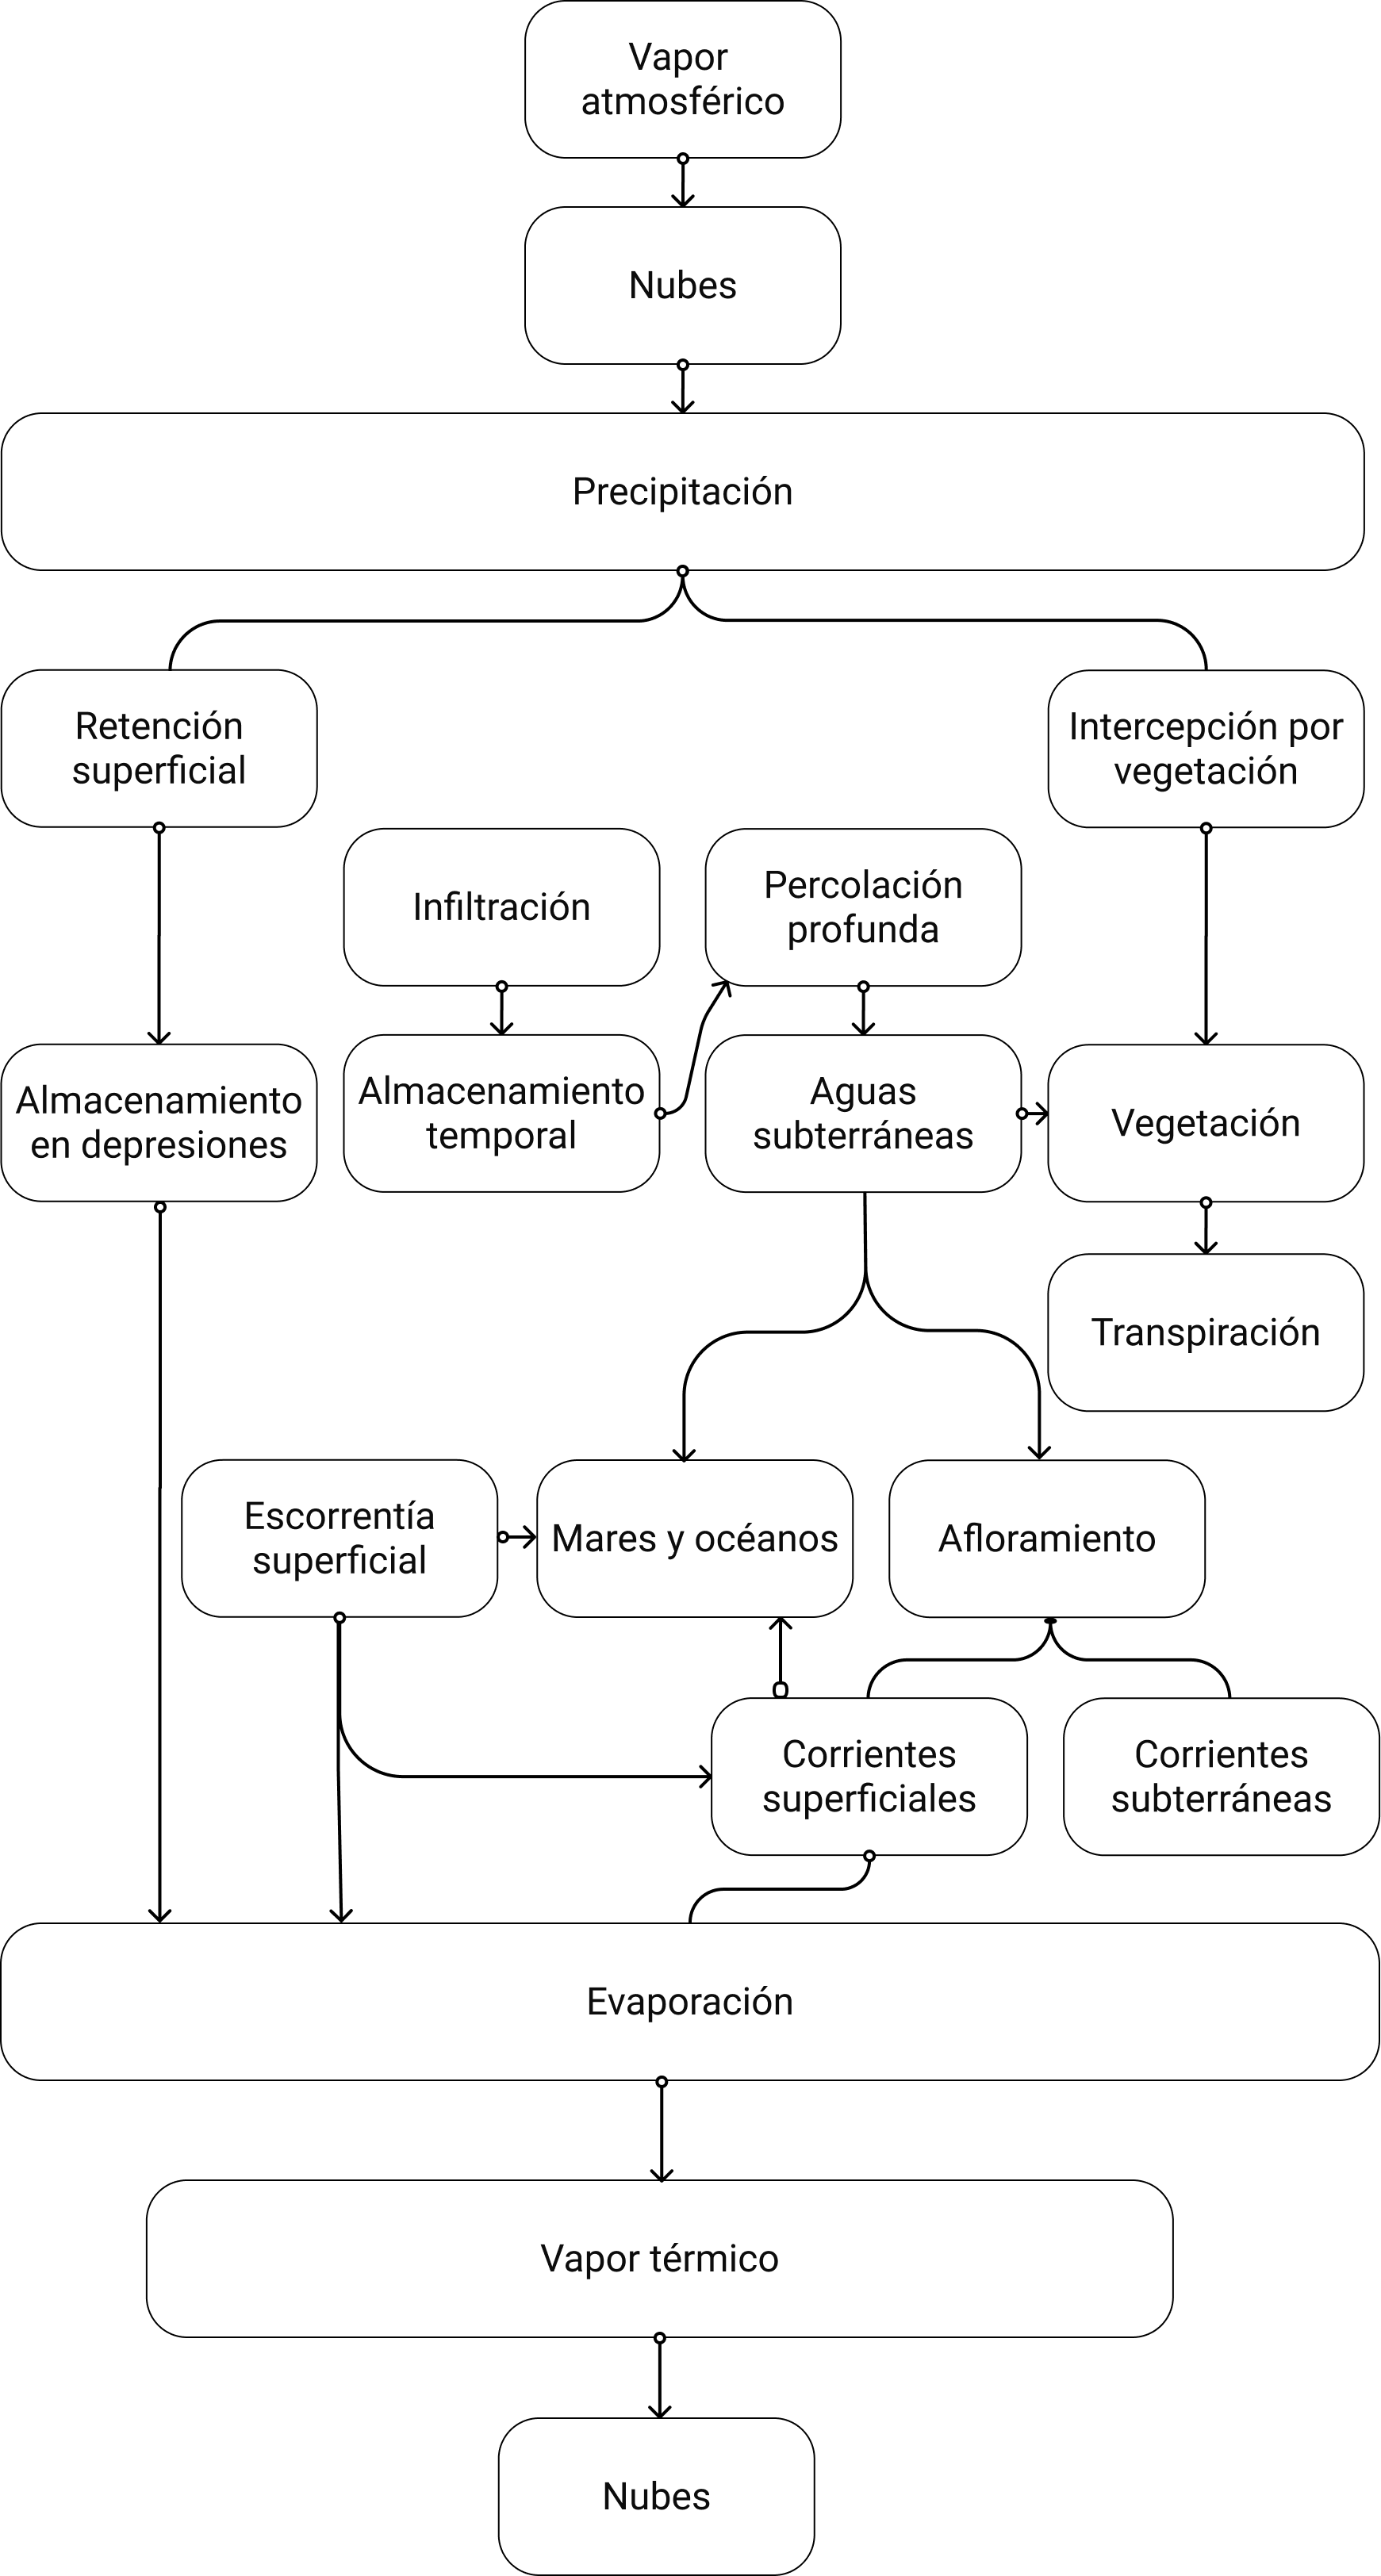
\includegraphics[width=0.7\textwidth]{fii1.png}}
	\caption{ciclo del agua}
	\label{fii1}
\end{figure}
Se puede observar que en ciclo hidrológico (véase la figura \ref{fii1}) intervienen procesos complejos de evaporación, precipitación, transpiración, infiltración, percolación, afloramiento, almacenamiento y escurrimiento. Para representar el ciclo hidrológico, se han hecho diferentes diagramas, algunos meramente descriptivos como el mostrado en la figura \ref{fii4}.
\subsubsection{Evaluación del Ciclo Hidrológico.} \label{subsubciclohidro}
A nivel mundial la energía solar evapora y eleva alrededor de: $500,000 Km^3$ de agua de la superficie terrestre, de la cual 86\% son de los océanos y 14\% de suelos. Una cantidad equivalente se precipita en la superficie en forma de lluvia, nieve o granizo: de la cual 78\% cae en la superficie de los océanos, lagos y lagunas; 22\% cae en la superficie terrestre, esto significa que el sistema transfiere $38,800 Km^3$ de \textbf{agua} de los océanos a continentes.

Para completar el Ciclo, el agua puede regresar a los océanos en forma
de escurrimiento.
\begin{figure}[h!]
	\centering
	\begin{subfigure}[b]{0.4\linewidth}
		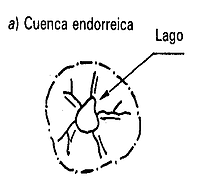
\includegraphics[width=\linewidth]{fii2.png}
		\caption{Una cuenca es una zona de la superficie terrestre en donde (si fuera impermeable) las gotas de lluvia que caen sobre ella tienden a ser drenadas por el sistema de corrientes hacia un mismo punto de salida.}
		\label{fii2}
	\end{subfigure}
	\begin{subfigure}[b]{0.4\linewidth}
		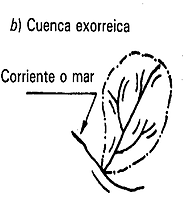
\includegraphics[width=\linewidth]{fii3.png}
		\caption{El punto de salida está dentro de los límites de la cuenca y generalmente es un lago.}
		\label{fii3}
	\end{subfigure}
	\caption{Su punto de salida está en los límites de las cuencas y está en
		otra corriente o mar.}
	\label{fig2-3}
\end{figure}
\begin{figure}[h!]
	\centerline{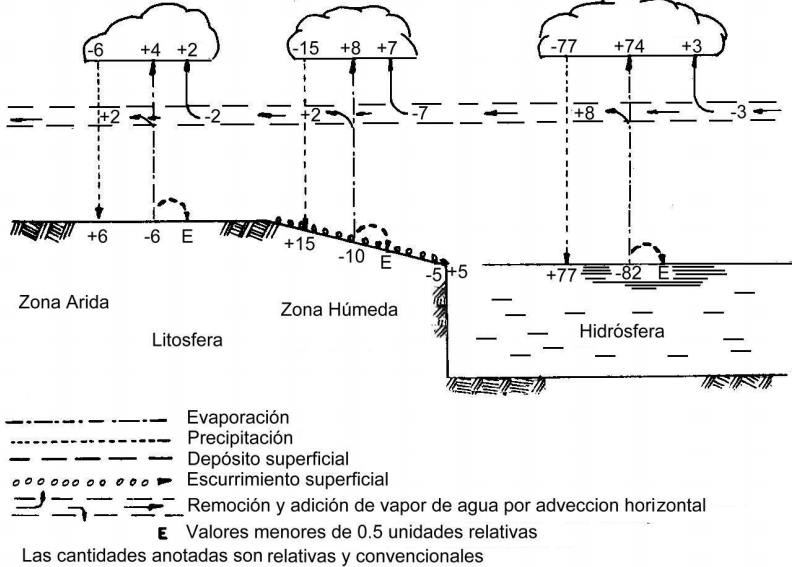
\includegraphics[width=0.7\textwidth]{fii4.png}}
	\caption{Representación cuantitativa del ciclo hidrológico.}
	\label{fii4}
\end{figure}
En México, la precipitación media anual es de 780 mm equivalente a $1,530 Km^3$, distribuida en forma genérica: $\frac{2}{3}$ partes en el sur y $\frac{1}{3}$ parte en el norte del país y concentrada en los meses de junio a octubre. De la anterior precipitación, el 68\% se evapotranspira, el 5\% se infiltra o percola recargando acuíferos, y el restante 27\% escurre superficialmente, representando un volumen de 410,000 millones de $m^3$, definido como \textbf{escurrimiento superficial virgen}, distribuido de la siguiente forma: en el 30\% de la superficie del país, en la zona norte, se genera tan solo el 4\% del escurrimiento, mientras que en el 20\% del territorio, en la zona sudeste y zonas costeras, se genera el 50\% del escurrimiento. Estas irregularidades espaciales y temporales plantean un reto especial en el manejo del agua de nuestro país.

Haciendo un balance del escurrimiento superficial, primeramente, a nivel regional, Los datos a nivel nacional están en la tabla \ref{tabone}
\begin{table}[h!]
	\centering
	\begin{tabular}{|c|c|c|c|c|c|c|}
		\hline
		\multicolumn{3}{|c|}{Disponibilidad Hídrica}                            & \multirow{3}{*}{\begin{tabular}[c]{@{}c@{}}Extracción\\ Para Usos\\ Consuntivos\end{tabular}} & \multirow{3}{*}{Exportac.(*)} & \multirow{3}{*}{Evaporación} & \multirow{3}{*}{Balance}                    \\ \cline{1-3}
		\multirow{2}{*}{\begin{tabular}[c]{@{}c@{}}Esc. \\ Virgen\end{tabular}} & \multirow{2}{*}{\begin{tabular}[c]{@{}c@{}}Retor.\\ Utiliz\end{tabular}}                      & \multirow{2}{*}{Import. (*)}  &                              &                          &          &       \\
		                                                                        &                                                                                               &                               &                              &                          &          &       \\ \hline
		410.7                                                                   & 2.98                                                                                          & 1.93                          & 49.2                         & 0.43                     & de Vasos & 357.6 \\ \hline
	\end{tabular}
	\caption{Balance del Agua Superficial en la República Mexicana (en $Km^3$/año) (*) Se importan de E.U. 1.85 $Km^3$ /año a la región noroeste y 0.07 a la región Norte y se exportan a E.U. 0.43 de la región Norte, comprometidos mediante el Acuerdo de carácter Internacional, así como 47.0 importados de Guatemala en la región sureste, sobre los cuales no existe convenio. El resto en importaciones y exportaciones son transferencias entre cuencas nacionales.}
	\label{tabone}
\end{table}
\subsection{Clasificación del Temporal}
Considerando la principal fase básica del ciclo hidrológico: la precipitación, y de
la cual dependen todas las \textbf{zonas de temporal}, en las que para producir alimentos,
se requiere de un temporal adecuado. Tomando solo en cuenta las condiciones medias anuales \autocite{Muñoz1976} de:
\begin{itemize}
	\item La precipitación pluvial
	\item y la temperatura
\end{itemize}
En un intento inicial el temporal ha sido clasificado, como en la tabla \ref{tabtwo} :
\begin{table}[h!]
	\centering\begin{tabular}{|l|l|l|l|}
		\hline
		\centering
		No & TIPO DE TEMPORAL & PRECIPITACIÓN          & TEMPERATURA                                                                                                                                                \\ \hline
		1  & EFICIENTE        & $> 700 mm$             & Entre 20 y 29$^{\circ}$C                                                                                                                                   \\ \hline
		2  & DEFICIENTE       & Entre $400$ y $700 mm$ & Entre 10 y 20$^{\circ}$C                                                                                                                                   \\ \hline
		3  & MALO             & $< 400 mm$             & \begin{tabular}[c]{@{}l@{}}Menor de 10 $^{\circ}$C y\\ Mayor de 29 $^{\circ}$C \end{tabular} \\ \hline
	\end{tabular}
	\caption{Clasificación del Temporal de acuerdo a la Precipitación y Temperatura.}
	\label{tabtwo}
\end{table}
\subsubsection{División del Territorio Nacional según su Precipitación}
En la república mexicana, las lluvias están irregularmente distribuidas durante los meses del año y en ocasiones hay localidades donde la precipitación de un mes cae en un solo día. Más del 65\% de la lluvia anual se presenta en solo cuatro meses, de junio a septiembre. Desafortunadamente, la ausencia de lluvias coincide frecuentemente con la máxima demanda de humedad por las plantas, lo que acentúa la condición de aridez de muchas regiones, independientemente de la reducida magnitud de la precipitación. Con excepción de Baja California y, en parte, de la costa de Sonora y Sinaloa, el régimen pluvial dominante se caracteriza por un periodo seco de noviembre a mayo y otros con lluvias de junio a octubre.

Además de ser el monto total de la lluvia, en general escaso durante el año y mal distribuido en los diversos meses, con frecuencia se presentan uno o varios años consecutivos de sequías.

Por lo que se refiere a las escasas lluvias invernales, estas provienen, en México, de masas de aire polar que descienden desde Canadá e invaden casi todo el país, causando algunas lluvias, frentes fríos y heladas. En el verano, al país llegan de ambos mares, vientos muy cargados de humedad que producen importantes lluvias, tanto en las cuencas de los ríos de la vertiente del Golfo como en la del Pacifico, y aún en la altiplanicie, lo que determina que las corrientes situadas, sobre todo en dichas vertientes, produzcan escurrimientos de consideración en esa época.

México recibe también la influencia de los ciclones tropicales, los cuales se forman durante el verano en los mares cálidos, próximos al Ecuador.

En la figura \ref{fii5} se muestra esquemáticamente cómo se distribuyen las lluvias en la república mexicana.
\begin{figure}[h!]
	\centerline{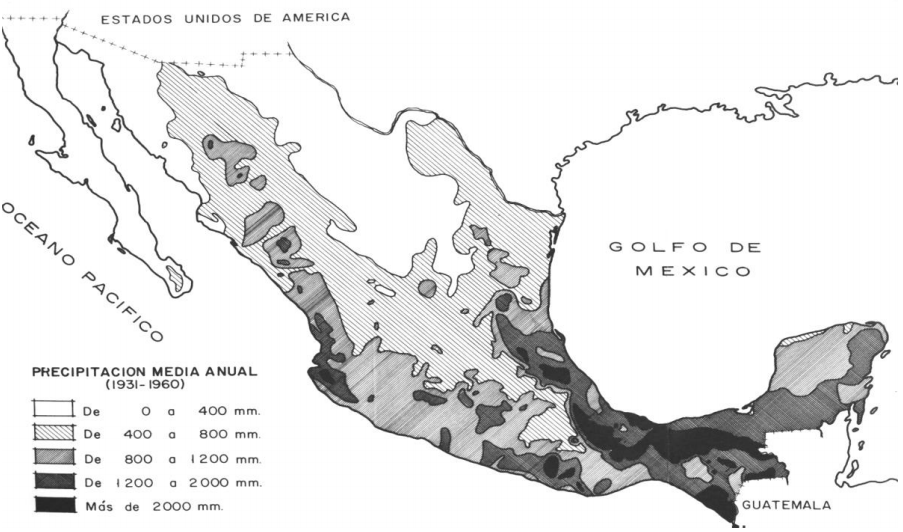
\includegraphics[width=1\textwidth]{fii5.png}}
	\caption{División del Territorio Nacional según la precipitación.}
	\label{fii5}
\end{figure}
\subsubsection{Formas de clasificación del Territorio nacional de acuerdo a la necesidad de Irrigación.}
De acuerdo al monto anual, distribución mensual de las lluvias, temperaturas y humedad atmosférica, el territorio nacional \autocite{Orive1970}, (según la necesidad de irrigación), se puede clasificar de acuerdo a la Tabla \ref{tabtree}:
\begin{table}[h!]
	\centering
	\begin{tabular}{|c|c|c|}
		\hline
		No  & Tipo de temporal   & Observaciones                                                                                                                                                                                                                        \\ \hline
		1   & Zona Húmeda        & No se requiere de la irrigación                                                                                                                                                                                                      \\ \hline
		2   & Zona Árida         & Sólo hay agricultura si aplicamos irrigación                                                                                                                                                                                         \\ \hline
		3   & Zonas Intermedias: & \begin{tabular}[c]{@{}c@{}}Las lluvias permiten el desarrollo\\ de cultivos sin necesidad de la irrigación.\end{tabular}                                                                                                             \\ \hline
		3.1 & Zona Semihúmeda    & \begin{tabular}[c]{@{}c@{}}Más del 50\% de los años, la lluvia es suficiente para\\ obtener una cosecha sin irrigación.\end{tabular}                                                                                                 \\ \hline
		3.2 & Zona semiárida     & \begin{tabular}[c]{@{}c@{}}Predominan los años con periodos de lluvias\\ insuficientes, se requiere el riego de auxilio\\ durante la temporada de lluvias, haciéndose\\ indispensable el riego en la temporada de secas\end{tabular} \\ \hline
	\end{tabular}
	\caption{Forma de clasificación del territorio Nacional según la necesidad de
		Irrigación.}
	\label{tabtree}
\end{table}
\subsubsection{Comparación de los estudios realizados sobre la necesidad de irrigación.}
Con posterioridad al estudio de 1944 de la Comisión Nacional de Irrigación (CNI), en 1958 la Secretaria de Recursos Hidráulicos hizo un nuevo estudio con mayor acopio de datos, acerca del panorama de México desde el punto de vista de la necesidad de irrigación. En 1961 la UNAM realizó otro estudio donde consideraba el índice de aridez de Emberger y por último en 1969 donde se racionalizaba el primer estudio subdividiendo las zonas extremas (Tabla \ref{tabfour}).
\begin{table}[h!]
	\centering
	\begin{tabular}{|c|c|c|c|c|c|c|c|}
		\hline
		\multicolumn{2}{|c|}{\begin{tabular}[c]{@{}c@{}}Estudio\\de 1944\end{tabular}} & \multicolumn{2}{c|}{\begin{tabular}[c]{@{}c@{}}Estudio\\de 1958\end{tabular}} & \multicolumn{2}{c|}{\begin{tabular}[c]{@{}c@{}}Estudio\\de 1961\end{tabular}} & \multicolumn{2}{c|}{\begin{tabular}[c]{@{}c@{}}Estudio de\\ 1969\end{tabular}}                                                                                    \\ \hline
		ZONA                                                                           & \%                                                                            & ZONA                                                                          & \%                                                                             & ZONA       & \%     & ZONA                                                  & \% \\ \hline
		Árida                                                                          & 52{.}1                                                                        & \begin{tabular}[c]{@{}c@{}}Riego\\ Indispensable\end{tabular}                 & 62{.}8                                                                         & Desértica  & 4{.}3  & \begin{tabular}[c]{@{}c@{}}Muy\\Árida \end{tabular}   & 23 \\ \hline
		\begin{tabular}[c]{@{}c@{}}Semi-\\árida\end{tabular}                           & 30{.}6                                                                        & \begin{tabular}[c]{@{}c@{}}Riego\\ Necesario\end{tabular}                     & 31{.}2                                                                         & Árida      & 33{.}9 & Árida                                                 & 20 \\ \hline
		\begin{tabular}[c]{@{}c@{}}Semi-\\humeda\end{tabular}                          & 10{.}5                                                                        & \begin{tabular}[c]{@{}c@{}}Riego \\ Conveniente\end{tabular}                  & 4{.}5                                                                          & semiárida  & 33{.}4 & semiárida                                             & 34 \\ \hline
		Húmeda                                                                         & 6{.}8                                                                         & \begin{tabular}[c]{@{}c@{}}Riego\\Inecesario\end{tabular}                     & 1{.}5                                                                          & Transición & 11{.}7 & \begin{tabular}[c]{@{}c@{}}Semi-\\humeda\end{tabular} & 16 \\ \hline
		\multicolumn{4}{|c|}{\multirow{3}{*}{}}                                        & \begin{tabular}[c]{@{}c@{}}Semi-\\húmeda\end{tabular}                         & 10{.}4                                                                        & Húmeda                                                                         & 4                                                                                \\ \cline{5-8}
		\multicolumn{4}{|c|}{}                                                         & Húmeda                                                                        & 4{.}8                                                                         & \begin{tabular}[c]{@{}c@{}}Muy\\húmeda\end{tabular}                            & 3                                                                                \\ \cline{5-8}
		\multicolumn{4}{|c|}{}                                                         & \begin{tabular}[c]{@{}c@{}}Muy\\Humeda\end{tabular}                           & 1{.}5                                                                         & \multicolumn{2}{c|}{}                                                                                                                                             \\ \hline
	\end{tabular}
	\caption{Comparación de estudios sobre la necesidad de irrigación en
		México }
	\label{tabfour}
\end{table}

%\begin{table}[h!]
%  \begin{tabular}{|c|c|c|c|c|c|c|c|}
%  \hline
%  \multicolumn{2}{|c|}{Estudio de 1944}  & \multicolumn{2}{c|}{Estudio de 1958}                                    & \multicolumn{2}{c|}{\begin{tabular}[c]{@{}c@{}}Estudio de\\ 1961\end{tabular}}   & \multicolumn{2}{c|}{Estudio de 1969} \\ \hline
%  ZONA                 & \%              & ZONA                                                           & \%     & ZONA                                      & \%                                   & ZONA                  & \%           \\ \hline
%  Árida                & 52{.}1          & Riego Indispensable                                            & 62{.}8 & Desértica                                 & 4{.}3                                & Muy Árida             & 23           \\ \hline
%  semiárida            & 30{.}6          & Riego Necesario                                                & 31{.}2 & Árida                                     & 33{.}9                               & Árida                 & 20           \\ \hline
%  Semihúmeda           & 10{.}5          & Riego Conveniente                                              & 4{.}5  & semiárida                                & 33{.}4                                & semiárida             & 34           \\ \hline
%  Húmeda               & 6{.}8           & \begin{tabular}[c]{@{}c@{}}No se necesita\\ Riego\end{tabular} & 1{.}5  & Transición                                & 11{.}7                               & Semihúmeda            & 16           \\ \hline
%  \multicolumn{4}{|c|}{\multirow{3}{*}{}}                                                                           & Semihúmeda                               & 10{.}4                               & Húmeda                & 4            \\ \cline{5-8} 
%  \multicolumn{4}{|c|}{}                                                                                            & Húmeda                                    & 4{.}8                               & MuyHúmeda             & 3            \\ \cline{5-8} 
%  \multicolumn{4}{|c|}{}                                                                                            & Muy Húmeda                                & 1{.}5                               & \multicolumn{2}{c|}{}                \\ \hline
%  \end{tabular}
%  \caption{Comparación de estudios sobre la necesidad de irrigación en
%  México }
%  \label{tabfour}
%\end{table}

Con los datos de lluvias, temperaturas, evaporaciones, etc$\dots$ Aportados por las estaciones climatológicas existentes en el país, así como los aportados por las nuevas estaciones que se instalen y los procedimientos tecnológicos que se desarrollen, será posible que se emprendan nuevos estudios, para los que Orive (1970) recomienda que se consideren las siguientes zonas, tomando las mismas dos zonas “límites”, o sea aquellas en que no puede haber agricultura si no hay riego, y aquellas en que no se necesita la irrigación para obtener una cosecha; para las zonas intermedias recomienda considerar a cinco, tal como se muestra en la Tabla \ref{tabfive}.
\begin{table}[h!]
	\centering
	\begin{tabular}{|c|c|}
		\hline
		ZONA & CARACTERÍSTICAS                                                                                                                                                                                                                                                                                                          \\ \hline
		I    & \begin{tabular}[c]{@{}c@{}}Donde el riego sea \\ absolutamente indispensable\end{tabular}                                                                                                                                                                                                                                \\ \hline
		II   & \begin{tabular}[c]{@{}c@{}}Donde del 0 al 20\% de los años \\ sea probable obtener una cosecha de\end{tabular}                                                                                                                                                                                                           \\ \hline
		III  & temporal (secano)                                                                                                                                                                                                                                                                                                        \\ \hline
		IV   & \begin{tabular}[c]{@{}c@{}}Donde la probabilidad sea \\ del 20\% al 40\% de los años\end{tabular}                                                                                                                                                                                                                        \\ \hline
		V    & Donde sea del 40\% al 60\%                                                                                                                                                                                                                                                                                               \\ \hline
		VI   & \begin{tabular}[c]{@{}c@{}}Donde la probabilidad \\ sea del 60\% al 80\%\end{tabular}                                                                                                                                                                                                                                    \\ \hline
		VII  & \begin{tabular}[c]{@{}c@{}}Donde sea del 80\% al 100\% Donde todos los años sea \\ probable obtener una cosecha\\ de temporal y por lo tanto el riego básicamente no se\\  necesite (pero en que muy\\ probablemente serán necesarias costosas obras \\ de desagüe y drenaje)\textbackslash{}end\{tabular\}\end{tabular} \\ \hline
	\end{tabular}
	\caption{Recomendación de zonas para futuros estudios sobre la necesidad de irrigación}
	\label{tabfive}
\end{table}

\subsubsection{Terrenos con posibilidades de aprovechamiento para el desarrollo agrícola de México.}
Se estima que las tierras llanas, o sea aquellas que tienen una pendiente menor del 10 \% tienen una superficie que, en números redondos, es del orden de unos 70 millones de hectáreas. Los terrenos con pendiente hasta de 25\% se han estimado en 140 millones de hectáreas. La distribución aproximada de las superficies anteriores para las cuatro zonas en que se ha dividido a México por su aridez, se muestra en la Tabla\ref{tabsix} :
\begin{table}[h!]
	\centering
	\begin{tabular}{|c|c|c|c|}
		\hline
		\multirow{2}{*}{ZONAS}                                                                                                                                                        & \begin{tabular}[c]{@{}c@{}}Con\\ Pendiente\\ de 0 a 10\%\\ Planas\end{tabular} & \begin{tabular}[c]{@{}c@{}}Con pendiente de\\ 10\% a 25\%\\ Obras de\\ Conservación de\\ Suelos\\ Fundamentales\end{tabular} & TOTAL \\ \cline{2-4}
		                                                                                                                                                                              & \multicolumn{3}{c|}{(en millones de ha)}                                                                                                                                                                              \\ \hline
		\begin{tabular}[c]{@{}c@{}}Áridas: Solo con riego puede\\ haber agricultura.\end{tabular}                                                                                     & 45                                                                             & 35.0                                                                                                                         & 80.0  \\ \hline
		\begin{tabular}[c]{@{}c@{}}semiáridas: Riego necesario\\ para eliminar lo aleatorio.\end{tabular}                                                                             & 12.5                                                                           & 17.5                                                                                                                         & 30.0  \\ \hline
		\begin{tabular}[c]{@{}c@{}}Semihúmedas: Temporal posible\\ en la mayoría de los años, pero\\ riego conveniente para eliminar\\ riesgos.\end{tabular}                          & 8.0                                                                            & 12.0                                                                                                                         & 20.0  \\ \hline
		\begin{tabular}[c]{@{}c@{}}Húmedas: Son indispensables\\ obras de drenaje y desagüe.\\ Riego de Auxilio en muchos casos\\ conveniente para cultivos\\ intensivos\end{tabular} & 4.5                                                                            & 5.5                                                                                                                          & 10.0  \\ \hline
		Sumas                                                                                                                                                                         & 70.0                                                                           & 70.0                                                                                                                         & 140.0 \\ \hline
	\end{tabular}
	\caption{Terrenos que serían aprovechables para el desarrollo agrícola de México}
	\label{tabsix}
\end{table}
Desde el punto de vista de la Irrigación, la superficie que es de interés es la de labor o laborable, la que se ha definido de acuerdo a los siguientes factores:
\begin{itemize}
	\item La limitación de los terrenos en lo correspondientes a pendientes no mayores del 10\%.
	\item La Escasez y mala distribución de las lluvias.
	\item Lo accidentado de su topografía.
	\item Lo erosionado de muchos suelos
	\item Su mal drenaje.
	\item La excesiva concentración salina de algunas tierras en las regiones áridas y semiáridas.
\end{itemize}
De acuerdo a estos factores se observa en la tabla \ref{tabseven}:
\begin{table}[h!]
	\centering
	\begin{tabular}{|l|l|l|}
		\hline
		\multirow{2}{*}{\textbf{Clasificación}}                 & \multicolumn{2}{l|}{\textbf{Superficie}}               \\ \cline{2-3}
		                                                        & \textbf{(en millones de ha)}             & \textbf{\%} \\ \hline
		De labor y laborable                                    & 29.3                                     & 14.9        \\ \hline
		Pastos en llanuras y lomeríos                           & 16.6                                     & 8.5         \\ \hline
		Pastos en terrenos cerril                               & 69.0                                     & 35.2        \\ \hline
		Superficie Forestal                                     &                                          & 33.7        \\ \hline
		Superficie inútil, no beneficiable para la agricultura. & 66.1                                     & 7.7         \\ \hline
		SUMAS:                                                  & 15.4                                     & 100.0       \\ \hline
	\end{tabular}
	\caption{Clasificación de la superficie del Territorio Nacional.}
	\label{tabseven}
\end{table}
Es necesario que se revisen las anteriores superficies tomando en cuenta la posibilidad de que, en un futuro no muy distante, se puedan llegar a eliminar, modificar o corregir algunos de los factores limitantes antes citados, gracias a una tecnología más avanzada y teniéndose en cuenta la presión que ejercerán las futuras e imperiosas necesidades de México, de que aumente su producción agrícola, no solo incrementando los rendimientos, sino también la superficie cultivable con buenas probabilidades de éxito.
\subsubsection{Superficie regable estimada en el territorio nacional.}
En un estudio realizado por la Secretaria de Recursos Hidráulicos en el año 1959, se hicieron las siguientes hipótesis para determinar el potencial agrícola con fines de riego en México, detalladas por Orive.
\begin{enumerate}
	\item Que el máximo aprovechamiento del agua superficial se logre construyendo presas de almacenamiento con las que se pueda llegar a utilizar el 75\% del volumen medio anual.
	\item Que se empleen los siguientes coeficientes de riego:
	      \begin{itemize}
		      \item Para climas desérticos y áridos: 12 000 $m^3/ha$
		      \item Para climas semi-áridos: 11,000 $m^3/ha$
		      \item Para climas semi-húmedos: 10,000 $m^3/ha$
		      \item Para climas húmedos: 9,000 $m^3/ha$
	      \end{itemize}
	\item Del agua aprovechada, ocurran retornos con valor del 20\% y que de estos retornos sea factible volver a aprovechar el 50\%.
\end{enumerate}
La superficie resultante se muestra en la Tabla \ref{tabeight}, se observa que el total de Área Neta Regable resulta de 11.45 millones de hectáreas la cual puede variar dependiendo de nuevos factores que puedan ser introducidos en el desarrollo del aprovechamiento del agua en México, que permiten prever que la superficie cultivable con agua segura puede ser mayor a la citada por Orive. Uno de estos estriba en la posibilidad de avanzar en la posibilidad de llevar aguas de cuencas donde existen más recursos hidráulicos que tierras que regar, a cuencas en que esta condición es la contraria, permitiría regar más superficie. En la tabla \ref{tabeight}, se consideró que con los retornos podía regarse una superficie de cerca de 800,000 hectáreas.
\begin{table}[h!]
	\centering
	\begin{tabular}{|c|c|c|c|c|c|}
		\hline
		\multirow{3}{*}{ZONA} & \multicolumn{2}{c|}{\begin{tabular}[c]{@{}c@{}}Agua superficial\\ media anual\end{tabular}} & \multirow{2}{*}{\begin{tabular}[c]{@{}c@{}}Área regable\\ hidrológicamente\end{tabular}} & \multirow{2}{*}{\begin{tabular}[c]{@{}c@{}}Área laborable\\ disponible\end{tabular}} & \multirow{2}{*}{\begin{tabular}[c]{@{}c@{}}Área neta\\ regable\end{tabular}}              \\ \cline{2-3}
		                      & Total                                                                                       & 75\%                                                                                     &                                                                                      &                                                                              &            \\ \cline{2-6}
		                      & \multicolumn{2}{c|}{Millones de $m^3$}                                                      & ha                                                                                       & ha                                                                                   & ha                                                                                        \\ \hline
		Desértica y árida     & 63,255                                                                                      & 47,441                                                                                   & 3,953,420                                                                            & 10,918,700                                                                   & 3,953,420  \\ \hline
		semiárida             & 49,363                                                                                      & 37,022                                                                                   & 3,365,640                                                                            & 7,139,700                                                                    & 3,365,640  \\ \hline
		Semihúmeda            & 5,811                                                                                       & 4,358                                                                                    & 435,800                                                                              & 1,511,000                                                                    & 435,800    \\ \hline
		Húmeda                & 238,848                                                                                     & 179,136                                                                                  & 19,909,000                                                                           & 3,696,500                                                                    & 3,696,500  \\ \hline
		TOTALES:              & 357,277                                                                                     & 267,927                                                                                  & 27,663,860                                                                           & 23,175,900                                                                   & 11,451,360 \\ \hline
	\end{tabular}
	\caption{Superficie regable estimada, según un estudio de 1959}
	\label{tabeight}
\end{table}
A través de varios años se han hecho diferentes consideraciones y estudios acerca de la potencialidad de México, en lo que corresponde a superficie factible y recursos hidrológicos disponibles \autocite{Cardenas1964}, para determinar el área máxima regable, los más importantes son los que se muestran en la Tabla \ref{tabnine}.
\begin{table}[h!]
	\centering
	\begin{turn}{90}
		\begin{tabular}{|c|c|c|c|c|c|c|}
			\hline
			\multirow{6}{*}{INVESTIGADOR}                                                     & \multirow{6}{*}{\begin{tabular}[c]{@{}c@{}}AÑO\\ DEL\\ ESTUDIO\end{tabular}} & \multicolumn{5}{c|}{S U P E R F I C I E S}                                                                                                                                                                                                                                                                                                                                       \\ \cline{3-7}
			                                                                                  &                                                                              & \multicolumn{2}{c|}{REGABLES}                                                   & \multirow{5}{*}{\begin{tabular}[c]{@{}c@{}}Riego\\ de\\ Auxilio\\ o \\ Humedad\end{tabular}} & \multirow{5}{*}{\begin{tabular}[c]{@{}c@{}}Riego\\ con\\ Aguas\\ de \\ Retorno\end{tabular}} & \multirow{2}{*}{\begin{tabular}[c]{@{}c@{}}TOTALES\\ en Ha\end{tabular}}                         \\ \cline{3-4}
			                                                                                  &                                                                              & \multirow{4}{*}{\begin{tabular}[c]{@{}c@{}}Aguas \\ superficiales\end{tabular}} & \multirow{4}{*}{\begin{tabular}[c]{@{}c@{}}Aguas\\ del\\ Subsuelo\end{tabular}}              &                                                                                              &                                                                          &                       \\ \cline{7-7}
			                                                                                  &                                                                              &                                                                                 &                                                                                              &                                                                                              &                                                                          &                       \\ \cline{7-7}
			                                                                                  &                                                                              &                                                                                 &                                                                                              &                                                                                              &                                                                          & \multicolumn{1}{l|}{} \\ \cline{7-7}
			                                                                                  &                                                                              &                                                                                 &                                                                                              &                                                                                              &                                                                          & \multicolumn{1}{l|}{} \\ \hline
			\begin{tabular}[c]{@{}c@{}}Adolfo Orive\end{tabular}                              & 1949                                                                         & 6 709 500                                                                       & 1 000 000                                                                                    & 2 291 500                                                                                    &                                                                          & 10 000 000            \\ \hline
			multirow{2}{*}{\begin{tabular}[c]{@{}c@{}}Rodríguez\\  Alba Antonio\end{tabular}} & 1957                                                                         & 10 000 000                                                                      & 2 700 000                                                                                    & 2 000 000                                                                                    &                                                                          & 14 700 000            \\ \hline
			Jorge L. Tamayo                                                                   & 1958                                                                         & 5 934 456                                                                       & 3 090 000                                                                                    & 2 000 000                                                                                    & 775 486                                                                  & 11 024 456            \\ \hline
			Andrés García Q.                                                                  & 1959                                                                         & 7 754 860                                                                       & 5 467 300                                                                                    & 3 696 500                                                                                    &                                                                          & 17 694 146            \\ \hline
			S.R.H.                                                                            & 1969                                                                         & 8 200 000                                                                       & 3 000 000                                                                                    &                                                                                              &                                                                          & 11 200 000            \\ \hline
		\end{tabular}
	\end{turn}
	\caption{Estudios realizados para la determinación de la Superficie Máxima
		Regable en México }
	\label{tabnine}
\end{table}
\subsection{Desarrollo de la Irrigación en diversas partes del mundo}

El origen de la agricultura bajo riego se pierde en la prehistoria más antigua. Algunos estudios muestran la utilización de la irrigación en Egipto hace 4,000 años, así como en China e igualmente en el Valle de Mesopotamia y en la India. En Egipto, en la actualidad las aguas del Nilo riegan aproximadamente 2,428,200 ha de tierras, que gran parte de estas son las mismas que se regaban antiguamente. Aquí existe la presa más antigua del mundo (hace 5,000 años) de 108 m de longitud y 12 m de altura.

En China, el riego lo utilizaban desde el año 2,627 años antes de Cristo (A.C.); en el siglo VII, D.C. se construyó un canal de 1,126 Km que fue usado primero en la navegación y después para el riego. Mucha superficie de tierra que en aquella época se regaba todavía da buenas cosechas en la actualidad. La presa Tu-Kiang actualmente sigue funcionando, fue construida por un hombre llamado Li y su hijo en los tiempos de la dinastía Chin (2,000 A.C.) y riega una extensión de más de 200,000 ha de arrozales.

En la región de Mesopotamia, en Asia Menor, los valles formados por los ríos Tigris y Eufrates, existen restos de antiguos de canales de riego, dos de ellos son los más largos de todos los tiempos, mostrando una gran habilidad en la irrigación de las civilizaciones antiguas.

En la India, existen presas en Ceylán (hoy Sri Lanka), que tienen más de 2,000 años. Testimonios de 300 años A.C. indican que el país se encontraba completamente regado y su prosperidad era muy grande a causa de las dos cosechas que podían colectar al año. En el sudoeste de Estados Unidos se evidencian restos de una civilización antigua basada en la agricultura de riego, trazos de antiguos canales son visibles todavía a lo largo del río Gila en Arizona.
\subsubsection{Distribución geográfica de la principal superficie de riego en el mundo.}
En el año 2012, la distribución geográfica de la principal superficie de riego en el mundo, de acuerdo a la FAO, tabla \ref{tabten}:
\begin{table}[h!]
	\centering
	\begin{tabular}{|c|c|c|}
		\hline
		No & PAÍS       & \begin{tabular}[c]{@{}c@{}}SUPERFICIE\\ (Millones de ha)\end{tabular} \\ \hline
		1  & INDIA      & 67                                                                    \\ \hline
		2  & CHINA      & 65                                                                    \\ \hline
		3  & USA        & 26                                                                    \\ \hline
		4  & PAKISTÁN   & 20                                                                    \\ \hline
		5  & IRÁN       & 8.4                                                                   \\ \hline
		6  & INDONESIA  & 7.5                                                                   \\ \hline
		7  & MÉXICO     & 6.5                                                                   \\ \hline
		8  & TAILANDIA  & 6.4                                                                   \\ \hline
		9  & BANGLADESH & 5.1                                                                   \\ \hline
		10 & TURQUÍA    & 5.0                                                                   \\ \hline
		11 & BRASIL     & 4.7                                                                   \\ \hline
		12 & VIETNAM    & 4.6                                                                   \\ \hline
		13 & RUSIA      & 4.3                                                                   \\ \hline
		14 & UZBEKISTÁN & 4.3                                                                   \\ \hline
		15 & EGIPTO     & 3.7                                                                   \\ \hline
		16 & IRAK       & 3.6                                                                   \\ \hline
		17 & ESPAÑA     & 3.4                                                                   \\ \hline
	\end{tabular}
	\caption{ Distribución geográfica de la principal superficie de riego en el mundo,
		al año 2012.}
	\label{tabten}
\end{table}
\subsubsection{Historia de la Irrigación en México}

\subsubsection*{La Irrigación Primitiva en México.}
Los Mexica se asentaron en el Valle de México cuando las enormes lagunas de Texcoco, Xochimilco, Chalco, Zumpango, etc$\dots$ ocupaban la mayor parte del valle. Estos lagos crecían y se desbordaban, por lo cual, para poder aprovechar sus aguas en usos urbanos, domésticos, así como para el riego, tuvieron que emprender una serie de acciones utilizando diques, canales, acueductos, presas, etc

Dentro de las anteriores acciones se encuentran también la llamada \textbf{``Chinampa''}, que es un campo de cultivo, jardín y habitación a la vez, aquí se llevan las tierras a las aguas. Estas están construidas con varas tejidas con raíces de plantas acuáticas y de otros materias ligeros, capaces de sostener unida la tierra de la Chinampa; sobre esta base se colocan ramas de las mismas plantas y encima el fango que sacan del fondo del lago, formando cuadriláteros de dimensiones variables.

Los trabajos de irrigación pre cortesanos, se deben a Netzahualcoyotl, estadista, poeta, filósofo y gran ingeniero que fue constructor del célebre vergel de Tezcutzingo y el dique o albarradón para dividir el lago de Texcoco (aguas saladas) del de México (aguas dulces), además de protegerlo contra las crecidas del mismo, evitando inundaciones.

El agua la conducían hacia los terrenos del regadío, desde lugares lejanos a través de acueductos llamados \textbf{``Apipilolli''} o por canales o acequias llamadas ``Apantli'', formando extensos sistemas de irrigación comunes a varios pueblos. En lugares propicios formaban grandes depósitos de agua de lluvias o albercas llamadas ``Tlaquilacaxitli'' a los que los españoles denominaron \textbf{``JAGÜEYES''}. En Cholula se encontraron restos de un acueducto de barro cocido de una sola pieza, con paredes de 30 cm de grueso, de sección toscamente circular con diámetro cercano a los 2m.
\subsubsection{Periodo Colonial}
La obra de colonización española estuvo encaminada a que las ciudades estuvieran abastecidas de agua, así como bien regados sus campos. Se hicieron vasos, acueductos, lagos artificiales, desviaciones de ríos y aprovechamientos de manantiales. En estas acciones se destacaron los frailes agustinos.

Los acueductos construidos durante esta época se cuentan por cientos; construidos con el objeto de regar los campos, huertos y para el abastecimiento de agua a poblaciones; entre estos se destacan: el de Epazoyucan de 15 Km de longitud, el de Tepeapulco de 23 Km, el acueducto de Guadalupe (12 Km y sustentado en 2310 arcos), los de Oaxaca, Morelia, Querétaro, Taxco, Chiapa de Corso, Atlacomulco, etc$\ldots$ En este periodo también se destacó la construcción de la Laguna de Yuriria por Fray Diego de Chávez, la cual es un hermoso lago artificial de 16 Km de largo por 6 Km de ancho.
\subsubsection{Periodo Independiente y Prerrevolucionario.}
En el último tercio del periodo se emprendieron algunas acciones como la construcción de algunas obras: La desecación de la Ciénaga de Chapala y los primeros canales de riego del Valle de Mexicali; obra de irrigación de Lombardía y Nueva Italia y diversos canales en la Comarca Lagunera.

Según lo detalla Orive, el único esfuerzo que se hizo por parte del gobierno de Porfirio Díaz para impulsar la construcción de obras de irrigación fue la creación en 1908 de “La Caja de Préstamos para Obra de Irrigación y Fomento de la Agricultura” con fundamento en la Ley del 17 de julio de 1908 facultando al ejecutivo para disponer de 25 millones de pesos del Tesoro Público con este fin.

Esta caja de Préstamos operó como Sociedad Anónima con un capital de 10 millones de pesos; emitió bonos con garantía del Gobierno federal por valor de 50 millones de pesos los que fueron colocados en el extranjero, e inició sus operaciones con más de 20 millones de pesos. Facilitaba fondos a grandes hacendados y a varias empresas agrícolas, ganaderas y hasta mineras, con garantía hipotecaria, interés de 7\% anual y plazo máximo de pago de 15 años. Los resultados de lo anterior fue que la mayoría de los deudores no cumplieron sus contratos y cuando las obras se ejecutaron, quedaron en manos de unos cuantos terratenientes que las explotaron en su beneficio personal.

\subsubsection{Periodo Posrevolucionario (Riego Institucional).}
En el periodo del año 1910 a 1915 se dio la etapa álgida de la lucha militar. Para 1915 en la ley del 6 de enero, se da la primera Ley Agraria, en la que se establecían una serie de derechos agrarios. Durante 1916, en la etapa final de construcción de la Presa Necaxa se presenta una falla en la cortina. En 1917, se presenta la Nueva Constitución Mexicana del 5 de febrero, mostrando en el artículo 27 su condición agraria, así como se presenta la terminación de la presa Boquilla (cortina de concreto y mampostería de 74 m de altura y 3,000 $Hkm^3$).

Para 1921, se crea la Dirección de Irrigación en la Secretaría de Agricultura y Fomento; esta Dirección se abocó a las siguientes acciones: a) Organización del Servicio Hidrológico, b) Estudio general de grandes proyectos (Yuriria y Tepuxtepec en el Lerma, el río Santiago en Aguascalientes, el Valle de Juárez en Chihuahua), c) Operación de obras de riego: Ciénaga de Chapala, Valle de Juárez y Canales del Yaqui. d) Construcción: reparación de canales Diaz, Marcos Carrillo y Vícam en el Valle del Yaqui, Reparación de diques y drenajes de la Ciénaga de Chapala y construcción de la presa Mexquitic en San Luis Potosí. En 1924 se crea la especialidad de Irrigación en la Escuela Nacional de Agricultura en San Jacinto, Distrito federal; así mismo se crea el departamento de Reglamentación e Irrigación, en sustitución de la dirección de Irrigación, con funciones notablemente reducidas y con raquítico presupuesto, funcionando así hasta 1925.

Para 1926 surge la Ley de Irrigación, reglamentando el uso de las aguas de propiedad Federal y se crea un nuevo organismo gubernamental: la Comisión Nacional de Irrigación (CNI). Esta comisión se enfrentó a dos grandes obstáculos por vencer: a) escasez de datos hidrométricos de las corrientes por aprovechar y b) la falta de personal especializado en el proyecto y construcción de las obras de irrigación. El primer obstáculo se decidió enfrentarlo construyendo dos obras: presa “Calles” y la Presa “Don Martín”, la primera con capacidad excesiva en su vaso y la segunda con una superficie proyecto de riego en forma excesiva. El segundo obstáculo, el gobierno resolvió no tratar de improvisar, sino traer a México un grupo brillante de ingenieros extranjeros, especializados en Irrigación, para lo cual la CNI estableció un contrato con empresas extranjeras para que estas, contando con los servicios de ingenieros verdaderamente especializados en el proyecto y la construcción de obras de riego, se encargarán de esos trabajos.

En el periodo de los años 1926 a 1928, se desarrolló la siguiente obra deirrigación: Presa Calles y la Presa Don Martín, así como la adaptación y reparación deobras construidas en el Distrito de Riego de Palestina, Coahuila para el riego de 1,600ha. Se adaptaron y ampliaron las obras de riego de Tula, para el riego de 33,800 ha. Seconstruyó la presa de Metztitlán, Hidalgo para el riego de 3,500 ha y se construyó laPresa Derivadora de Mante, Tamaulipas para regar 8,500 ha.
 
Para el periodo de los años 1929 a 1934, se construyó la siguiente obra de irrigación: Presa Abelardo Rodríguez en Baja California; obras de riego del Nogal, en Coahuila, que son aguas del río Sabinas, tributario del Salado, afluente del río Bravo; obras en Delicias, Chihuahua: Presa derivadora y canales; obras en Cd. Juárez: reacondicionamiento de canales y construcción de una red de drenes. En este periodo se pusieron bajo riego 146,600 ha.

En el periodo de los años de 1935 a 1940, se inició la construcción de grandes presas para irrigación: Presa El Palmito, en Durango, para el riego de 83,000 ha se inició en 1936 y se concluyó en 1946; la Presa Solis, en Guanajuato, para el riego de 102,500 ha se inició en 1939 y se concluyó en 1949; Presa Sanalona, en Sinaloa, para el riego de 94,000 ha se inició en 1939 y se concluyó en 1948; la Presa La Angostura, en Sonora, para el riego de 115,000 ha, se inició en 1936 y se concluyó en 1942 y la Presa Marte R. Gómez (El Azúcar) en Tamaulipas, para el riego de 66,000 ha, se inició en 1936 y concluyó en 1946.

Además se iniciaron las siguientes obras importantes: en Baja California, el mejoramiento de canales y drenes en el río Colorado; en Guerrero, una derivadora en el Río Cutzamala; en Hidalgo, la Presa Huichapan y canales en Ixmiquilpan; en Jalisco y Michoacán, obras de reforzamiento de diques y mejoramiento de drenes en la Ciénaga de Chapala; en Michoacán, la Presa Cointzio, canales y drenes en Morelia y Queréndaro, así como en Apatzingán; así como canales en diversos estados. La superficie puesta bajo riego (nueva y mejorada) en el periodo fue de 118,495 ha.

En este periodo se inicia la construcción de obras de pequeña irrigación (1937), para desarrollar infraestructura de riego en la altiplanicie mexicana. Para el periodo de los años de 1941 a 1946, como obra de irrigación se desarrolló la construcción de la Presa Abelardo Rodríguez en Sonora, y se continuó y concluyó buena parte de las iniciadas en el anterior periodo. En cuanto a la Pequeña Irrigación, la CNI construyó 66 obras con las que se puso bajo riego a 37,000 ha. En diciembre de 1946 se funda la Secretaria de Recursos Hidráulicos en sustitución de la CNI. La superficie puesta bajo riego (nueva y mejorada) en el periodo fue de 549,129 ha.

Durante el periodo de los años de 1947 a 1952, se construyeron las siguientes grandes presas: Álvaro Obregón en Sonora, para riego de 220,000 ha; Endo, en el río Tula en Hidalgo, para el riego de 5,000 ha; Mocúzari, en Sonora, para riego de 60,000 ha. En este periodo la obra de pequeña irrigación fue muy importante incorporando al riego 146,442 ha, de las 652,512 ha de riego nuevas y mejoradas para el periodo.

En 1947, se creó la Comisión del Papaloapan con el objeto de planear, diseñar y construir las obras requeridas para el desarrollo integral y armónico de la cuenca del río Papaloapan. Así mismo en el mismo año se creó la Comisión del Tepalcatepec, con idénticas finalidades, para 1960 se transforma en la Comisión del Balsas. Para el año de 1952, se funda la Comisión del Río Fuerte, iniciándose la construcción de la Presa Miguel Hidalgo; igualmente en el mismo año se crea la Comisión del Río Grijalva.

En el periodo de los años 1953 al 1958, la principal obra de grande irrigación consistió en la construcción de: la Presa El Marqués, en Oaxaca; La Presa Falcón, en Tamaulipas. La obra de Pequeña Irrigación incorporó al riego 148,000 ha. La superficie beneficiada fue de 748,000 ha para el periodo, con obras nuevas y mejoradas. En 1958 se crea la Comisión de Estudios del Río Pánuco.

Para el periodo comprendido entre los años 1959 a 1964, la obra de irrigación realizada consistió en la Presa La Amistad en Coahuila y la Presa Humaya (López Mateos), en Sinaloa, para riego de 90,000 ha; en la obra de pequeña irrigación se incorporó una superficie de 110,000 ha haciendo un total de superficie beneficiada de 251,000 ha para el periodo, con obras nuevas y mejoradas. En 1960 se crea la Comisión de Estudios del Río Lerma. Durante el periodo de los años 1965 al 1970, se crearon los siguientes organismos:
\begin{enumerate}
	\item El \textbf{PLHINO} (Plan HIdráulico del Noroeste) que perseguía el aprovechamiento conjunto de 17 ríos con 25,000 millones de $m^3$ anuales, tratando de que la superficie de riego existente de 874,000 ha se incrementará en 426,000 ha haciendo un total de 1’300,000 ha.
	\item El \textbf{PLHICEN} (Plan HIdráulico del Centro), creado para solucionar el problema de abastecimiento de agua a la zona metropolitana de la Ciudad de México y subsecuente uso de las aguas residuales en el riego.
	\item \textbf{PLHIGON} (Plan HIdráulico del Golfo Norte), que perseguía el permitir el aprovechamiento conjunto de las aguas de cuatro importantes cuencas del Noreste de la República Mexicana: Pánuco, Purificación, San Fernando y Bravo, conduciendo agua del Pánuco hacia Matamoros.
	\item \textbf{PNPI} (Plan Nacional de Pequeña Irrigación) con el objeto de dotar de riego en 10 años a 306,000 ha.
	\item  Plan de mejoramiento de la eficiencia en el uso del agua, con el objeto de aumentar la eficiencia de conducción del 50\% al 65\% en promedio y la Parcelaria del 50\% al 70\% haciendo un total de 45\%, a este último se le denominó \textbf{PLAMEPA} (Plan de Mejoramiento Parcelario), tratando de mejorar el uso del agua en la parcela.
\end{enumerate}
En el año de 1972 se decreta la Ley Federal de Aguas; en 1975 se crea la \textbf{CPNH} (Comisión del Plan Nacional Hidráulico), que intentaba establecer un plan maestro para detectar zonas críticas carentes de agua, identificándose las siguientes:
\begin{itemize}
	\item Área Crítica No 1. Zona metropolitana de la Ciudad de México
	\item Área Crítica No 2. Cuenca Alta y Media del Río Lerma en lo referente a la Contaminación de las aguas.
	\item Área Crítica No 3. Zona metropolitana de la Ciudad de Monterrey.
\end{itemize}
Para el año 1977 se decreta la desaparición de la Secretarías de Agricultura y Ganadería y la de Recursos Hidráulicos, creándose una nueva dependencia de gobierno: la Secretaría de Agricultura y Recursos Hidráulicos (\textbf{SARH}). En este año desaparecen todas la Comisiones, exceptuando a la CPNH y la Comisión del Ex-lago de Texcoco, así mismo se funda la Dirección General de Distritos de Temporal.

En 1986 se crea el Instituto Mexicano de Tecnología del Agua (\textbf{IMTA}), en sustitución de la CPNH. Para 1989 se funda la Comisión Nacional del Agua (\textbf{CNA}) a partir de la Subsecretaria de Infraestructura Hidráulica de la SARH, iniciándose el proceso de privatización de los distritos de riego, entregando la operación de la infraestructura de riego a nivel de red menor a Asociaciones de Usuarios, y constituyéndose como autoridad federal única en la materia. En el año de 1992 se promulga la Ley de Aguas Nacionales, destacándose entre sus objetivos: a) La administración integral del agua, con una mayor participación de los usuarios y entidades federativas a través de los consejos de cuenca; b) El aprovechamiento eficiente y racional del agua para la modernización del agua para la modernización del campo y en general para la modernización del país; c) La mayor participación de particulares en la construcción y operación de la infraestructura y servicios hidráulicos; d)La seguridad jurídica en el uso y aprovechamiento del agua, que permita a los particulares planear adecuadamente sus actividades a mediano y largo plazos; entre otros. Durante el año 1993 se decretan reformas sustanciales al Artículo 27 Constitucional permitiendo entre otras acciones el arrendamiento y venta de terrenos ejidales, así como el otorgamiento de concesiones a particulares para el aprovechamiento y manejo de los recursos hidráulicos. En 1994 la CNA se integra a la secretaria del Medio Ambiente Recursos Naturales y Pesca (\textbf{SEMARNAP}) como órgano desconcentrado de esta, y como organismo ejecutor de la política hidráulica en México se crea en su interior, en el año de 1996 el Programa de Modernización del Manejo del Agua (\textbf{Promma}), como instancia para ejecutar el programa hidráulico 1995-2000.

\subsection{Problemática y retos de la Irrigación en México.}
Los grandes problemas que se presentan en la actualidad, respecto a la Irrigación en México, es por un lado la insuficiencia de infraestructura para dar atención a la gran demanda de alimentos ante el crecimiento poblacional, que hace que se esté importando buena parte de los granos básicos fundamentales para alimentación del pueblo, tal es el caso del Maíz, que se importa el 55\% del consumo nacional, así mismo con el frijol, trigo, arroz, etc$\ldots$ Por otro lado, es la sobre explotación de las fuentes de aguas superficiales y subterráneas, en las primeras simplemente se agota el recurso y mucha superficie con infraestructura de riego que deja de usarse, por ejemplo de una superficie de los distritos de riego de 3.5 millones de hectáreas solamente se riegan 2.2 millones de hectáreas. En lo que corresponde a la sobreexplotación de las aguas subterráneas, es el abatimiento de los niveles de los acuíferos que derivan a severos problemas de calidad, tal situación sucede en los acuíferos costeros que se presentan problemas de intrusión salina, que nulifican la utilización de los mismos; y en los acuíferos continentales la aparición de aguas fósiles, con severos problemas de la presencia de arsénico en el agua y otros metales pesados, que sin ser detectables a primera vista genera severos problemas de salud en las personas usuarias del agua de esos acuíferos$\ldots$

Así mismo, es la gran contaminación que generan lo grandes centros de población, en el uso del agua que deriva a severos problemas de calidad con residuales cada vez más agresivos y que al no recibir ningún tratamiento, y utilizarse en el riego deriva a grandes problemas de calidad en los productos agrícolas y más en el caso de aquellos que se consumen crudos, y es la causa y origen de severos problemas de salud en las personas.
\subsubsection{Patrimonio Hidráulico de México acreditado para el año 1998}
\begin{itemize}
	\item 4,500 presas de almacenamiento (Grandes, Medianas y Pequeñas)
	\item 2,597 presas derivadoras
	\item 54,000 millones de $m^3$ de capacidad útil para riego
	\item 80,000 millones de $m^3$ de almacenamiento total.
	\item 80,775 Km de canales
	\item 29,450 Km de drenes y desagües
	\item 60,826 Km de caminos de operación y enlace de zonas agrícolas.
	\item 3,350 plantas de bombeo
	\item 150,000 pozos profundos
	\item 210,000 estructuras en canales, drenes y caminos todo lo anterior para regar 6.2 millones de ha, con lo cual México ocupa el 8º. Lugar mundial por su infraestructura de riego.
	\item 2,700 Km de acueductos que entregan 2,840 millones de$ m^3$ al año de agua en bloque a poblaciones.
	\item 76.5 millones de habitantes (83.5\%) con agua potable.
	\item 61.4 millones de habitantes (67.0\%) con servicio de alcantarillado.
	\item 818 plantas de tratamiento de aguas residuales de origen municipal.
	\item 43,000 l/s de capacidad instalada total (24.7\% del caudal total de aguas residuales de origen municipal).
	\item 5,300 l/s de tratamiento de aguas residuales de origen industrial (8.3\% del caudal total de aguas residuales de origen industrial).
	\item Más de 100 plantas hidroeléctricas
	\item 8,171 MW de capacidad instalada total
	\item 21\% de la energía total generada.
\end{itemize}
\subsubsection{Superficie puesta bajo riego para diferentes años, en México.}

Hasta el año de 1910 la superficie que se encontraba bajo riego era de
aproximadamente de 700,000 ha, una vez que el estado toma bajo su responsabilidad a
través de la Comisión Nacional de Irrigación en 1926 y lo hecho hasta 1930 se
estimaba que la superficie de riego era de 1,000,000 ha; de 1926 a 1966 la CNI hasta
1946 y de aquí la Secretaría de Recursos Hidráulicos pusieron bajo riego 2,543,302 ha
haciendo un total de 3,543,302 ha para 1966, estudios posteriores mostraban como se
dio la superficie bajo riego en 1976, 1979 y 1985, tal como se muestra en la Tabla \ref{tab11}.

\begin{table}[h!]
	\centering
	\begin{tabular}{|c|c|c|c|}
		\hline
		\multirow{2}{*}{}                                                                                                                                                                                                         & \multicolumn{3}{c|}{SUPERFICIES EN ha}                                                                                                                                                                                    \\ \cline{2-4}
		                                                                                                                                                                                                                          & \begin{tabular}[c]{@{}c@{}}Al 29 de marzo\\ de 1976\end{tabular}      & \begin{tabular}[c]{@{}c@{}}Al 20 de marzo\\ de 1979\end{tabular}        & A Dic. de 1985                                                          \\ \hline
		\begin{tabular}[c]{@{}c@{}}Operadas y supervisadas como \\ distritos de riego\\ \\ Operadas y supervisadas como\\ Unidades de Riego para el\\ Desarrollo Rural\end{tabular}                                               & \begin{tabular}[c]{@{}c@{}}2,846,970\\ \\ \\ \\  803,000\end{tabular} & \begin{tabular}[c]{@{}c@{}}3,000,000\\ \\ \\ \\  1,223,000\end{tabular} & \begin{tabular}[c]{@{}c@{}}3,215,000\\ \\ \\ \\  1,554,000\end{tabular} \\ \hline
		TOTAL SARH:                                                                                                                                                                                                               & 3,649,970                                                             & 4,223,000                                                               & 4,769,000                                                               \\ \hline
		\begin{tabular}[c]{@{}c@{}}Operadas por particulares y\\ otras dependencias de Gobierno\\ (incluyendo 430,000 ha\\ operadas y supervisadas con\\ bombeo de agua del subsuelo)\\ \\ Operadas por particulares\end{tabular} & \begin{tabular}[c]{@{}c@{}}1,214,456\\ \\  --\end{tabular}            & \begin{tabular}[c]{@{}c@{}}--\\ \\  777,000\end{tabular}                & \begin{tabular}[c]{@{}c@{}}--\\ \\  8000,00\end{tabular}                \\ \hline
		\begin{tabular}[c]{@{}c@{}}Total de Superficie Puesta Bajo\\ Riego:\end{tabular}                                                                                                                                          & 4,864,426                                                             & 5,000,000                                                               & 5,569,000                                                               \\ \hline
	\end{tabular}
	\caption{Obra de Irrigación y superficie puesta bajo riego por Instituciones
		Gubernamentales y por Particulares.}
	\label{tab11}
\end{table}
Posteriormente se han dado cifras aisladas
mencionando que para fines de los años ochenta la superficie ya era de 6,000,000 ha y
así se mantuvo hasta que recientemente en 1998, se mencionó que la superficie total
era de 6.2 millones de hectáreas (según el Programa Hidráulico 1995-2000, CNA \autocite{federal1996programa}), otras
fuentes señalan a 6.3 millones de hectáreas, distribuida de acuerdo al Programa
Hidráulico 1995-2000 en: 3.3 millones de hectáreas ubicadas en 80 distritos de riego y
2.9 millones de hectáreas radicada en más de 39,600 unidades de mediano y pequeño
riego.

\subsubsection{Costos de una hectárea nueva bajo riego}

\begin{table}[h!]
	\centering
	\begin{tabular}{|c|c|}
		\hline
		Año  & Costo (*)/ha  \\ \hline
		1970 & \$ 10,500     \\ \hline
		1976 & \$ 56,000     \\ \hline
		1980 & \$ 70,000     \\ \hline
		1985 & \$ 1,200,000  \\ \hline
		1987 & \$ 2,300,000  \\ \hline
		1990 & \$ 7,500,000  \\ \hline
		1994 & \$ 26,000,000 \\ \hline
		1998 & \$ 90,000,000 \\ \hline
	\end{tabular}
	\caption{ Costo de una hectárea nueva bajo riego, en sistemas de riego por
		gravedad (incluye fuente de abastecimiento). (*) precios corrientes, en moneda nacional, de los respectivos años}
	\label{tab12}
\end{table}
\begin{table}[h!]
	\centering
	\begin{tabular}{|c|c|}
		\hline
		Tipo de Sistema de Riego                                                                                                                                        & Costo(USD)/ha                                                                  \\ \hline
		\begin{tabular}[c]{@{}c@{}}Entubado con compuertas\\ Entubado con compuertas y\\  válvula de intermitencias\\ Aspersión \\ Microaspersión \\ Goteo\end{tabular} & \begin{tabular}[c]{@{}c@{}}800\\ \\ 1,100\\ 1,500\\ 1,800\\ 2,100\end{tabular} \\ \hline
	\end{tabular}
	\caption{Costo de una hectárea nueva bajo riego, en sistemas de riego
		presurizados (sin Fuente de Abastecimiento).}
	\label{tab13}
\end{table}

La tabla \ref{tab013}, nos muestra la superficie de cultivo requerida para dar alimentación al pueblo mexicano, durante las próximas décadas, hasta el año 2030.
\begin{table}[h!]
	\centering
	\begin{tabular}{|c|c|c|c|c|}
		\hline
		\multirow{2}{*}{Concepto}                                                                        & \multicolumn{4}{c|}{AÑOS}                                                                                                                                                                                       \\ \cline{2-5}
		                                                                                                 & 2000                                               & 2010                                             & 2020                                               & 2030                                               \\ \hline
		Población Total (1)                                                                              & 99.9                                               & 113                                              & 126                                                & 137                                                \\ \hline
		ÁREA TOTAL DE CULTIVO (2)                                                                        & 20                                                 & 21                                               & 22                                                 & 23                                                 \\ \hline
		\begin{tabular}[c]{@{}c@{}}Área cultivada por (2)\\ área cultivada por temporal (2)\end{tabular} & \begin{tabular}[c]{@{}c@{}}6.3\\ 13.7\end{tabular} & \begin{tabular}[c]{@{}c@{}}7.0\\ 14\end{tabular} & \begin{tabular}[c]{@{}c@{}}7.8\\ 14.2\end{tabular} & \begin{tabular}[c]{@{}c@{}}8.5\\ 14.5\end{tabular} \\ \hline
		Área Cultivada por Habitante (3)                                                                 & 0.2                                                & 0.18                                             & 0.17                                               & 0.16                                               \\ \hline
	\end{tabular}
	\caption{(1) Millones de habitantes, (2) Millones de Hectáreas,(3) Hectáreas/habitante}
	\label{tab013}
\end{table}

En la tabla \ref{tab14} , nos muestra la situación de la agricultura, en lo que respecta a la producción de granos básicos en la república mexicana, a través de los decenios.

\begin{table}[h!]
	\centering
	\begin{tabular}{|c|c|c|c|}
		\hline
		AÑOS                                                                                                        & \begin{tabular}[c]{@{}c@{}}SUPERFICIE\\ TOTAL\\ COSECHADA\\ (ha)\end{tabular}                                                                                           & \begin{tabular}[c]{@{}c@{}}NUMERO DE\\ HABITANTES\end{tabular}                                                                                                          & \begin{tabular}[c]{@{}c@{}}SUPERFICIE\\ COSECHADA POR\\ HABITANTE\\ (ha/hab)\end{tabular}                   \\ \hline
		\begin{tabular}[c]{@{}c@{}}1910\\ 1921\\ 1930\\ 1940\\ 1950\\ 1960\\ 1970\\ 1980\\ 1990\\ 1997\end{tabular} & \begin{tabular}[c]{@{}c@{}}5,770,000\\ 5,150,000\\ 5,233 000\\ 5,904,000\\ 8,576,355\\  10,854,000\\  14 853 000\\  15,311,000\\  15,757,595\\  15,258,108\end{tabular} & \begin{tabular}[c]{@{}c@{}}15,160,000\\ 14,335,000\\ 16,553,000\\ 19,654,000\\ 25,791,000\\ 34,293,000\\ 48,225,000\\ 66,847,000\\ 83,750,000\\ 94,700,000\end{tabular} & \begin{tabular}[c]{@{}c@{}}0.38\\ 0.36\\ 0.32\\ 0.30\\ 0.33\\ 0.31\\ 0.31\\ 0.23\\ 0.19\\ 0.16\end{tabular} \\ \hline
	\end{tabular}
	\caption{Superficie Anual Cosechada por Habitante en la República Mexicana,
		en los decenios anteriores.}
	\label{tab14}
\end{table}


La FAO establece los siguientes parámetros para definir la condición de los
países en torno a su producción agrícola y la alimentación de sus pueblos \autocite{rudiño1999}:

\begin{itemize}
	\item Países con un valor de la Superficie Total Cosechada por Habitante menor
	      a 0.5 ha/hab: son incapaces de satisfacer sus necesidades y deben usar una
	      técnica agrícola adelantada para aumentar los rendimientos de los cultivos, o
	      subsistir a base de importaciones de productos agrícolas.
	\item Países con un valor de la Superficie Total Cosechada por Habitante
	      ubicado entre 0.5 y 1.0 ha/hab: Son capaces de satisfacer sus necesidades de
	      alimentación.
	\item Países con un valor de la Superficie Total Cosechada por Habitante mayor
	      a 1.0 ha/hab: Son capaces de exportar productos agrícolas.
\end{itemize}

\begin{table}[h!]
	\centering
	\begin{tabular}{|c|c|c|c|}
		\hline
		AÑOS                                                                         & MAÍZ & FRIJOL & TRIGO \\ \hline
		1930                                                                         & 190  & 30     & 2     \\
		1940                                                                         & 170  & 30     & 3     \\
		1950                                                                         & 170  & 40     & 4     \\
		1960                                                                         & 160  & 40     & 4     \\
		1970                                                                         & 150  & 40     & 3     \\
		1980                                                                         & 100  & 020    & 2     \\
		1990                                                                         & 088  & 250    & 13    \\
		1997                                                                         & 076  & 17     & 12    \\ \hline
		\begin{tabular}[c]{@{}c@{}}Producción \\ mínima\\ indispensable\end{tabular} & 156  & 23     & 13    \\ \hline
	\end{tabular}
	\caption{Superficie anual cosechada por habitante de algunos cultivos básicos para la alimentación de la población en Aguascalientes (en ha/hab).}
	\label{tab15}
\end{table}

\begin{table}[h!]
	\centering
	\begin{tabular}{|c|c|c|c|c|}
		\hline
		\textbf{AÑOS}                                                                                 & \textbf{MAÍZ}                                                                       & \textbf{FRIJOL}                                                             & \textbf{TRIGO}                                                                & \textbf{ARROZ}                                                        \\ \hline
		\begin{tabular}[c]{@{}c@{}}1930\\ 1940\\ 1950\\ 1960\\ 1970\\ 1980\\ 1990\\ 1997\end{tabular} & \begin{tabular}[c]{@{}c@{}}83\\ 83\\ 121\\ 155\\ 184\\ 185\\ 175\\ 185\end{tabular} & \begin{tabular}[c]{@{}c@{}}5\\ 5\\ 10\\ 15\\ 19\\ 14\\ 15\\ 10\end{tabular} & \begin{tabular}[c]{@{}c@{}}22\\ 24\\ 23\\ 34\\ 57\\ 42\\ 47\\ 37\end{tabular} & \begin{tabular}[c]{@{}c@{}}5\\ 5\\ 7\\ 9\\ 8\\ 7\\ 5\\ 5\end{tabular} \\ \hline
		\begin{tabular}[c]{@{}c@{}}Producción Mínima\\ Indispensable\end{tabular}                     & 180                                                                                 & 20                                                                          & 60                                                                            & 15                                                                    \\ \hline
	\end{tabular}
	\caption{Producción anual por habitante de algunos cultivos básicos para la
		alimentación de la población en la república mexicana (en Kg/hab).}
	\label{tab16}
\end{table}

\begin{figure}[h!]
	\centerline{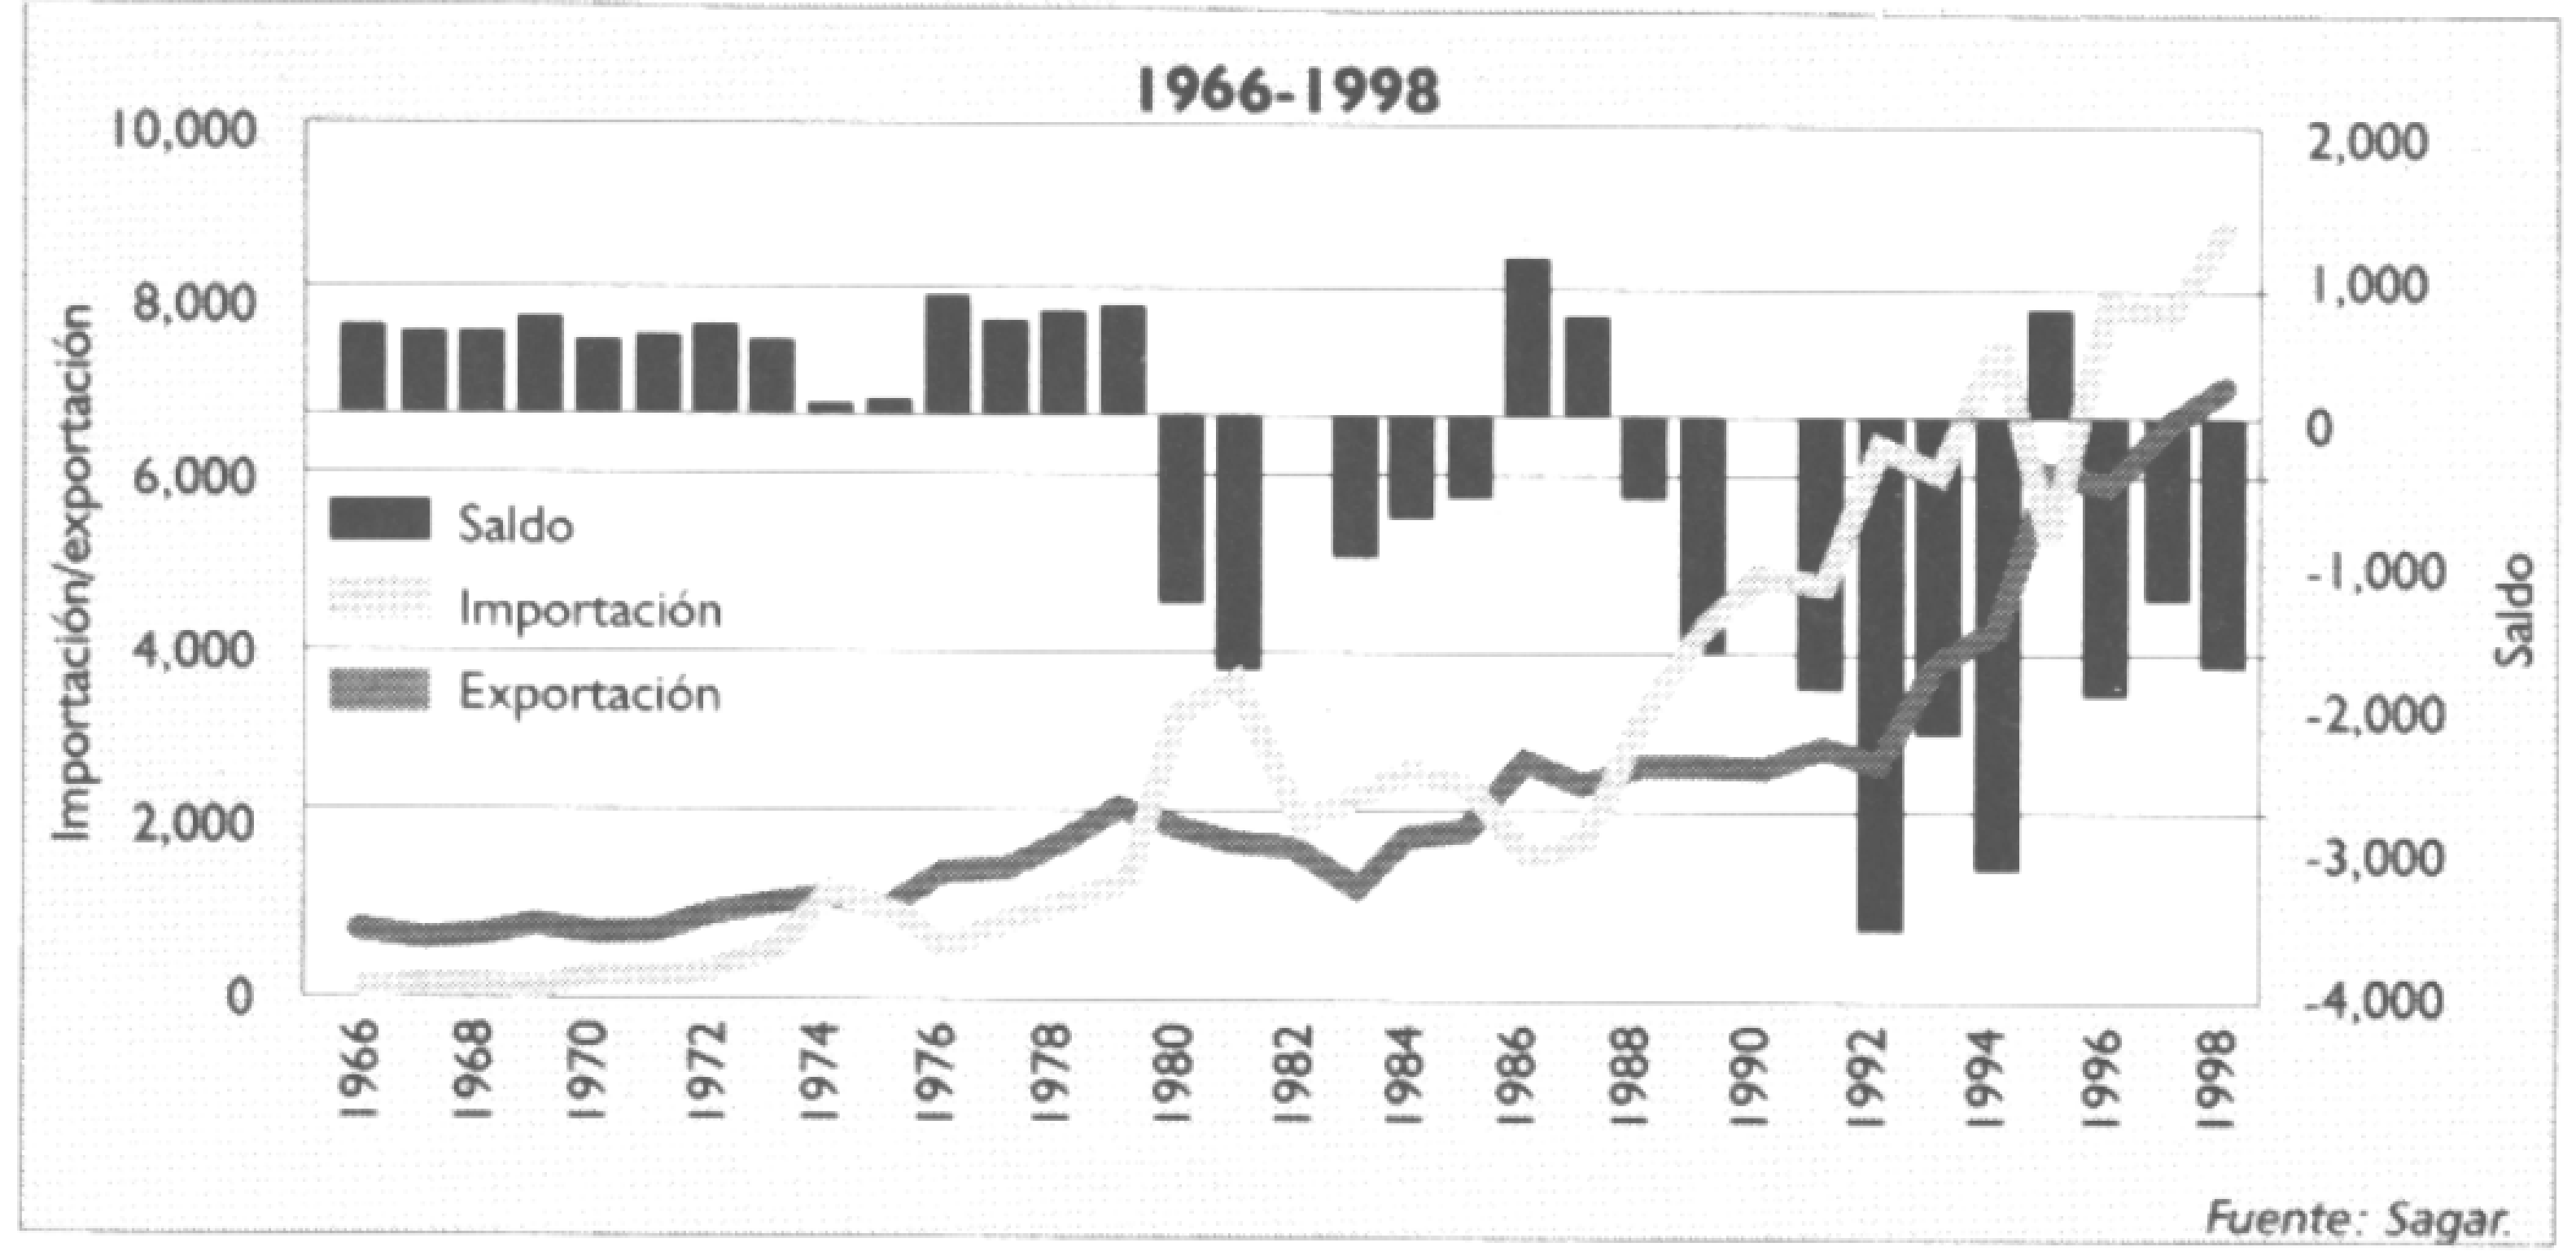
\includegraphics[width=0.7\textwidth]{fii6.png}}
	\caption{Balanza Comercial Agroalimentaria de México durante el periodo
		1966-1998 (en millones de dólares)}
	\label{fii6}
\end{figure}

\section{Manejo del agua}
El agua superficial consta de dos cuerpos distintos de agua en la naturaleza:
\begin{enumerate}
	\item El agua oceánica, la cual se encuentra altamente mineralizada por sales. El
	      cuerpo de agua oceánica contiene agua para cubrir todo el globo terráqueo; es la
	      principal fuente de humedad atmosférica y, por ende, de los demás cuerpos de agua
	\item  Los cuerpos superficiales de agua dulce, que cubren pequeñas porciones de
	      la superficie terrestre.
\end{enumerate}

El agua dulce se halla en ríos, depósitos y lagos; es almacenada durante el
invierno como nieve o hielo.
Aún en regiones caracterizadas por abundantes cuerpos de agua superficial, la
mayoría de las plantas, y por lo tanto, el hombre, no vivirían si el agua almacenada del
suelo no fuera útil para la conservación de las plantas. Tomando como promedio 1.5 m
de espesor de la zona que penetran las raíces, la humedad contenida en el suelo es
equivalente a poco menos de 30 cm de agua. El agua almacenada en el suelo está
adherida a las partículas del mismo y es removida en gran parte por la transpiración de
las plantas. Este déficit o pérdida debe ser repuesto antes de que el agua se pueda
mover hacia abajo, hasta el espejo del agua a través de la zona vacía del suelo. Por
consiguiente, la filtración del agua de lluvia no puede ser una fuente importante del
agua en regiones áridas.

La manifestación del agua superficial que permite ser aprovechada en lugares
alejados a donde se encuentra como ejemplo el caso de lagos y lagunas, es a través
del escurrimiento que se presenta en cauces de ríos o arroyos. El escurrimiento es el
agua proveniente de la precipitación que circula sobre o bajo la capa superficial del
suelo o en estratos más profundos y que llega a una corriente para finalmente ser
drenada hasta la salida de una cuenca. Existen tres tipos de escurrimiento: superficial,
subsuperficial y subterráneo.

La forma de aprovechar el agua superficial, en forma de escurrimiento, es a
través de diferentes obras de infraestructura que van a estar condicionadas a la forma
como se de el escurrimiento en los cauces, así si el escurrimiento es intermitente,
situación típica de zonas áridas y semiáridas, la forma de aprovechar esto es a través
de presas de almacenamiento auxiliadas con otras obras; si el escurrimiento es
permanente y este es de magnitud pequeña en la época de estiaje, la forma de
aprovechar este es a través de Presas derivadoras, situación típica en zonas
semihúmedas, y si el escurrimiento es permanente y la magnitud de este es de gran
tamaño, la forma de aprovechar estos es a través de tomas directas, esto es típico en
zonas húmedas.

\textbf{El almacenamiento de agua depende:}
\begin{itemize}
	\item Área y forma de la cuenca
	\item Precipitación en la cuenca (registros necesarios: Estaciones termopluviométricas)
	\item Escurrimientos superficiales (registros necesarios: Estaciones hidrométricas)
	\item Carácter geológico del sitio.
\end{itemize}

\textbf{Tipos de almacenamiento:}
\begin{itemize}
	\item Vasos en forma de lagos naturales (caso: Zacapu y Chapala, subirrigación)
	\item Vasos en cuencas de drenaje natural (presas de almacenamiento)
	\item Depresiones topográficas a las que debe conducirse el agua (importación de otra
	      cuenca)
	\item Almacenamientos puramente artificiales (bordos, jagüeyes)
\end{itemize}

\textbf{Selección del sitio para un almacenamiento:}
\begin{itemize}
	\item Proximidad
	\item Abastecimiento
	\item Topografía
	\item Geología
\end{itemize}

\textbf{Precauciones especiales que se deben tener al planear almacenamientos:}
\begin{itemize}
	\item Evitar depósitos de yeso
	\item Grietas o cavidades en regiones volcánicas
	\item Atención a areniscas de grano grueso
	\item Depresiones con relleno de acarreo
	\item Rellenos de grava y arena
	\item Investigación completa para evaluar abastecimiento, determinar fugas posibles, evitar desbordamientos
	\item Estudio de los suelos superficiales y subsuelo del vaso y la cuenca (azolve).
	\item Probar alternativas de obras de excedencias.
	\item Protección de la cuenca tributaria, con manejo adecuado evitando y previniendo
	      la deforestación.
\end{itemize}

\subsection{Aprovechamientos de aguas subterráneas.}

Las aguas subterráneas tienen su origen en la precipitación y en la parte de la
misma que se denomina infiltración, que es el movimiento vertical del agua, a través de
las capas superficiales del suelo, producido por la acción de las fuerzas gravitacionales
y capilares. Este proceso se presenta en la capa superficial del suelo que se denomina:
``Zona de Fractura de las Rocas'' la cual a su vez se subdivide en tres capas: la primera
denominada de evaporación en la cual el movimiento del agua que se infiltra se
caracteriza por dos movimientos uno descendente y otro ascendente, el primero hace
que el agua siga su proceso hacia capas inferiores del suelo, y el segundo que hace
que regrese de nuevo a la atmósfera fundamentalmente en forma de vapor. La segunda
capa que se denomina zona de aireación, en la cual el agua se encuentra en
combinación con el aire ocupando los poros existentes en el suelo, con un solo
movimiento vertical descendente que hace que continué su camino hacia abajo, a la
siguiente capa, que se denomina zona de saturación, en la cual el aire desaparece de
los poros y el agua ocupa exclusivamente el espacio que ellos dejan, conformando en
su parte superior lo que se denomina nivel freático, y en su parte inferior lo que se
denomina hidroapoyo concluyendo con la zona de fractura de las rocas, tal como se
observa en la Figura \ref{fii7}.


\begin{figure}[h!]
	\centering
	\begin{subfigure}[b]{0.45\linewidth}
		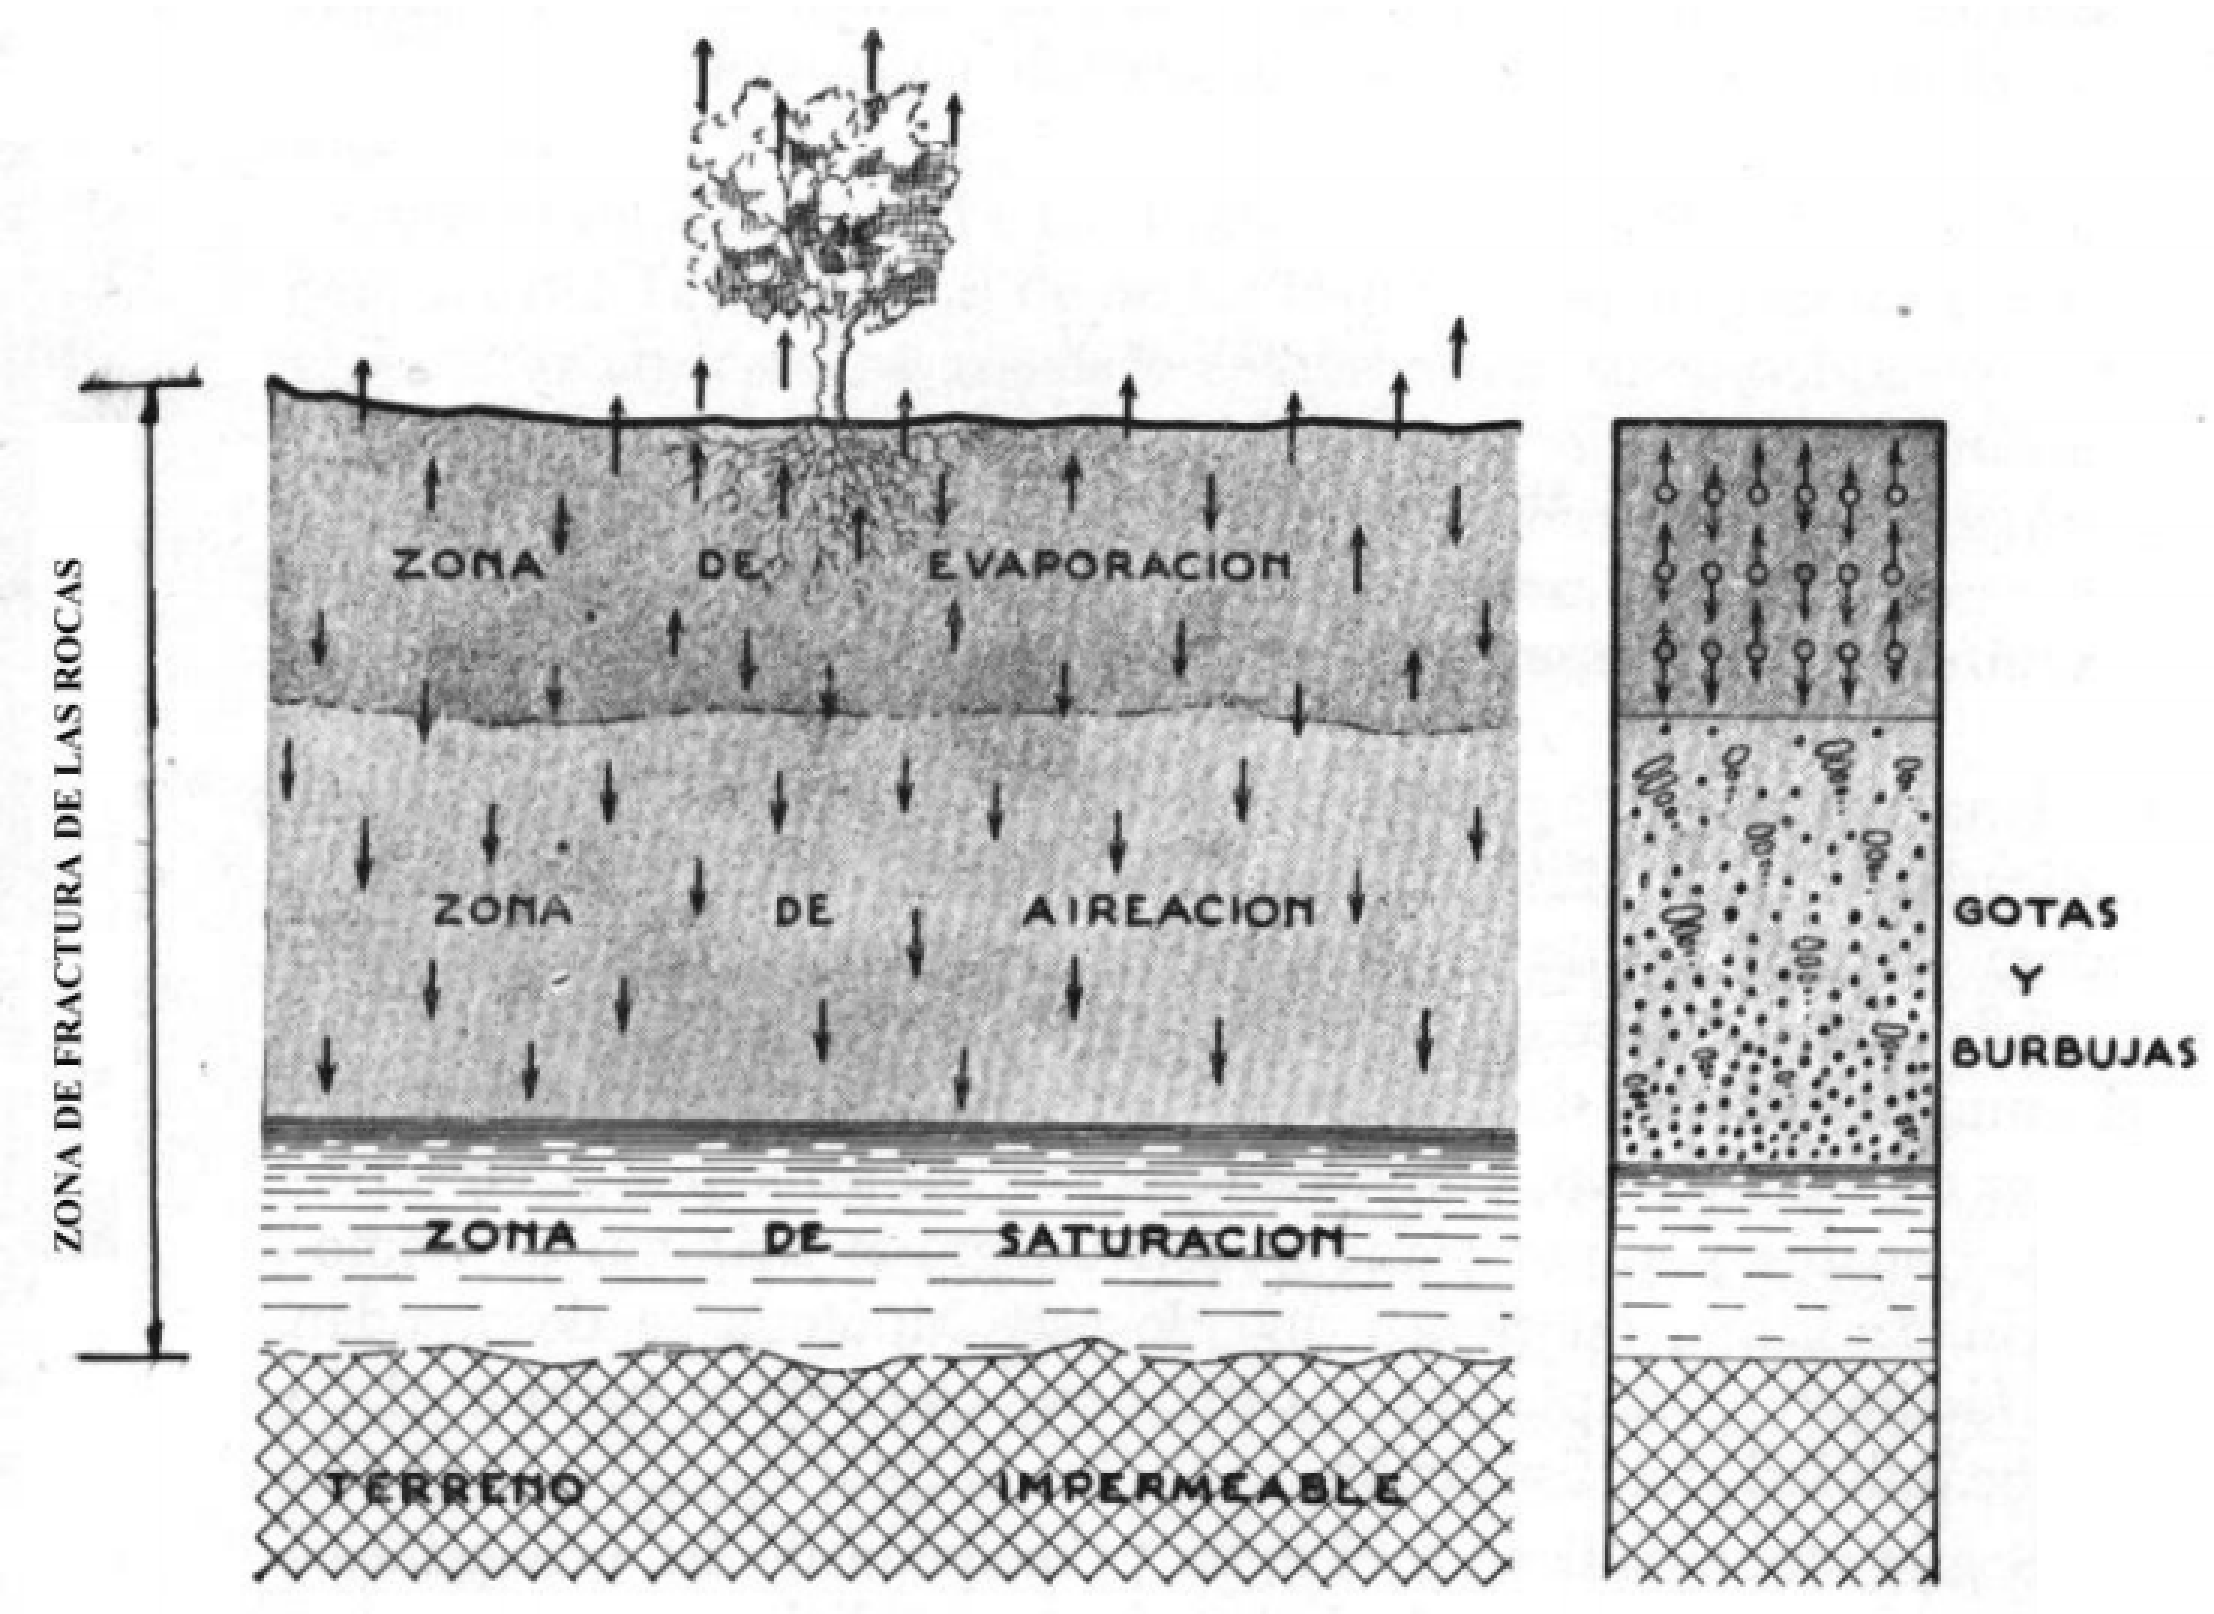
\includegraphics[width=\linewidth]{fii7.png}
		\caption{Capa superficial del movimiento del agua subterránea.}
		\label{fii7}
	\end{subfigure}
	\begin{subfigure}[b]{0.45\linewidth}
		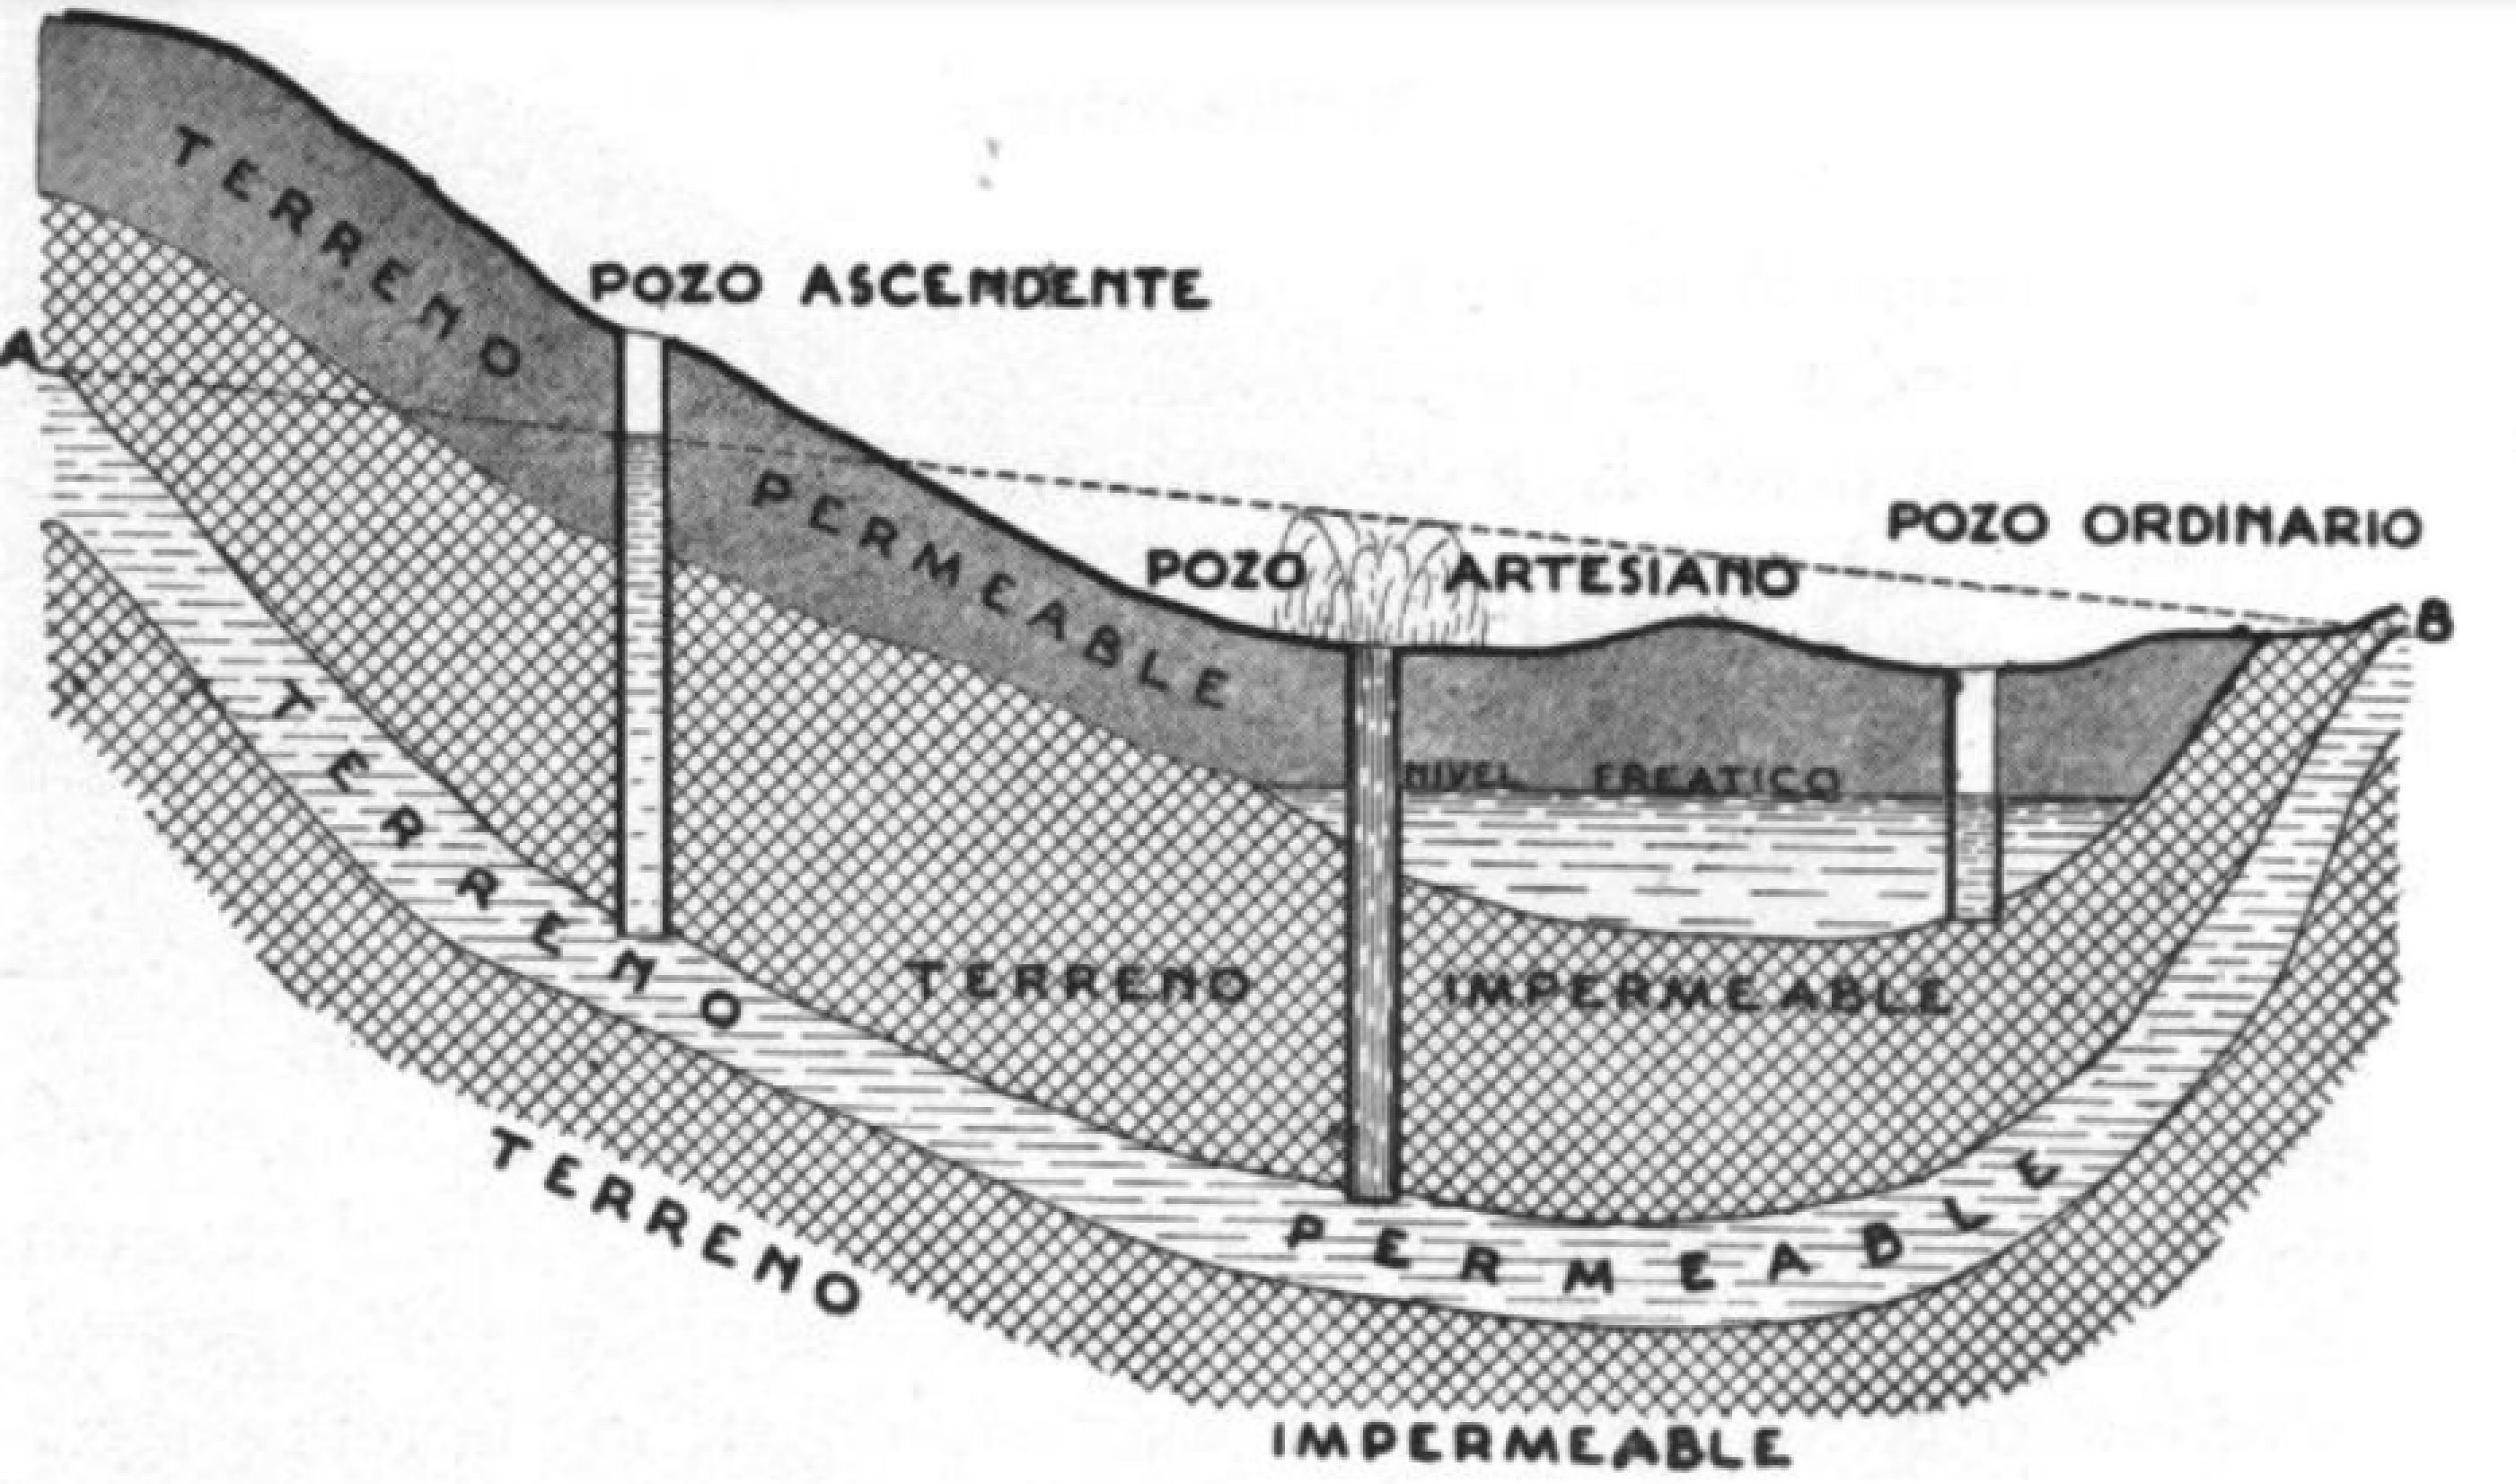
\includegraphics[width=\linewidth]{fii8.png}
		\caption{El punto de salida está dentro de los límites de la cuenca y generalmente es un lago.}
		\label{fii8}
	\end{subfigure}
	\caption{Formas de explotación artificial de las aguas subterráneas.}
	\label{fig7-8}
\end{figure}

\subsubsection{Tipos de alumbramiento de las aguas subterráneas.}

\begin{enumerate}
	\item Alumbramiento natural.
	      \begin{enumerate}
		      \item  Manantiales o fuentes
		            \begin{enumerate}
			            \item De afloramiento, derramamiento o vertedero.
			            \item De emergencia o de vaguada
			            \item De grieta o de filón
			            \item Intermitentes
			            \item  Intercalares
		            \end{enumerate}
	      \end{enumerate}
	\item Alumbramiento artificial
	      \begin{enumerate}
		      \item  Sentido vertical (pozos)
		            \begin{enumerate}
			            \item Pequeño diámetro (pozos profundos, taladros, perforaciones o
			                  pozos entubados).
			            \item Gran diámetro (a cielo abierto, pozos ordinarios o tipo noria).
			            \item Mixtos
		            \end{enumerate}
		      \item  Sentido horizontal (galerías).
		            \begin{enumerate}
			            \item Trincheras colectoras
			            \item Galerías filtrantes
			            \item Galerías de captación
			            \item Galerías en el fondo de pozos.
		            \end{enumerate}
	      \end{enumerate}
\end{enumerate}

\begin{figure}[h!]
	\centering
	\begin{subfigure}[b]{0.4\linewidth}
		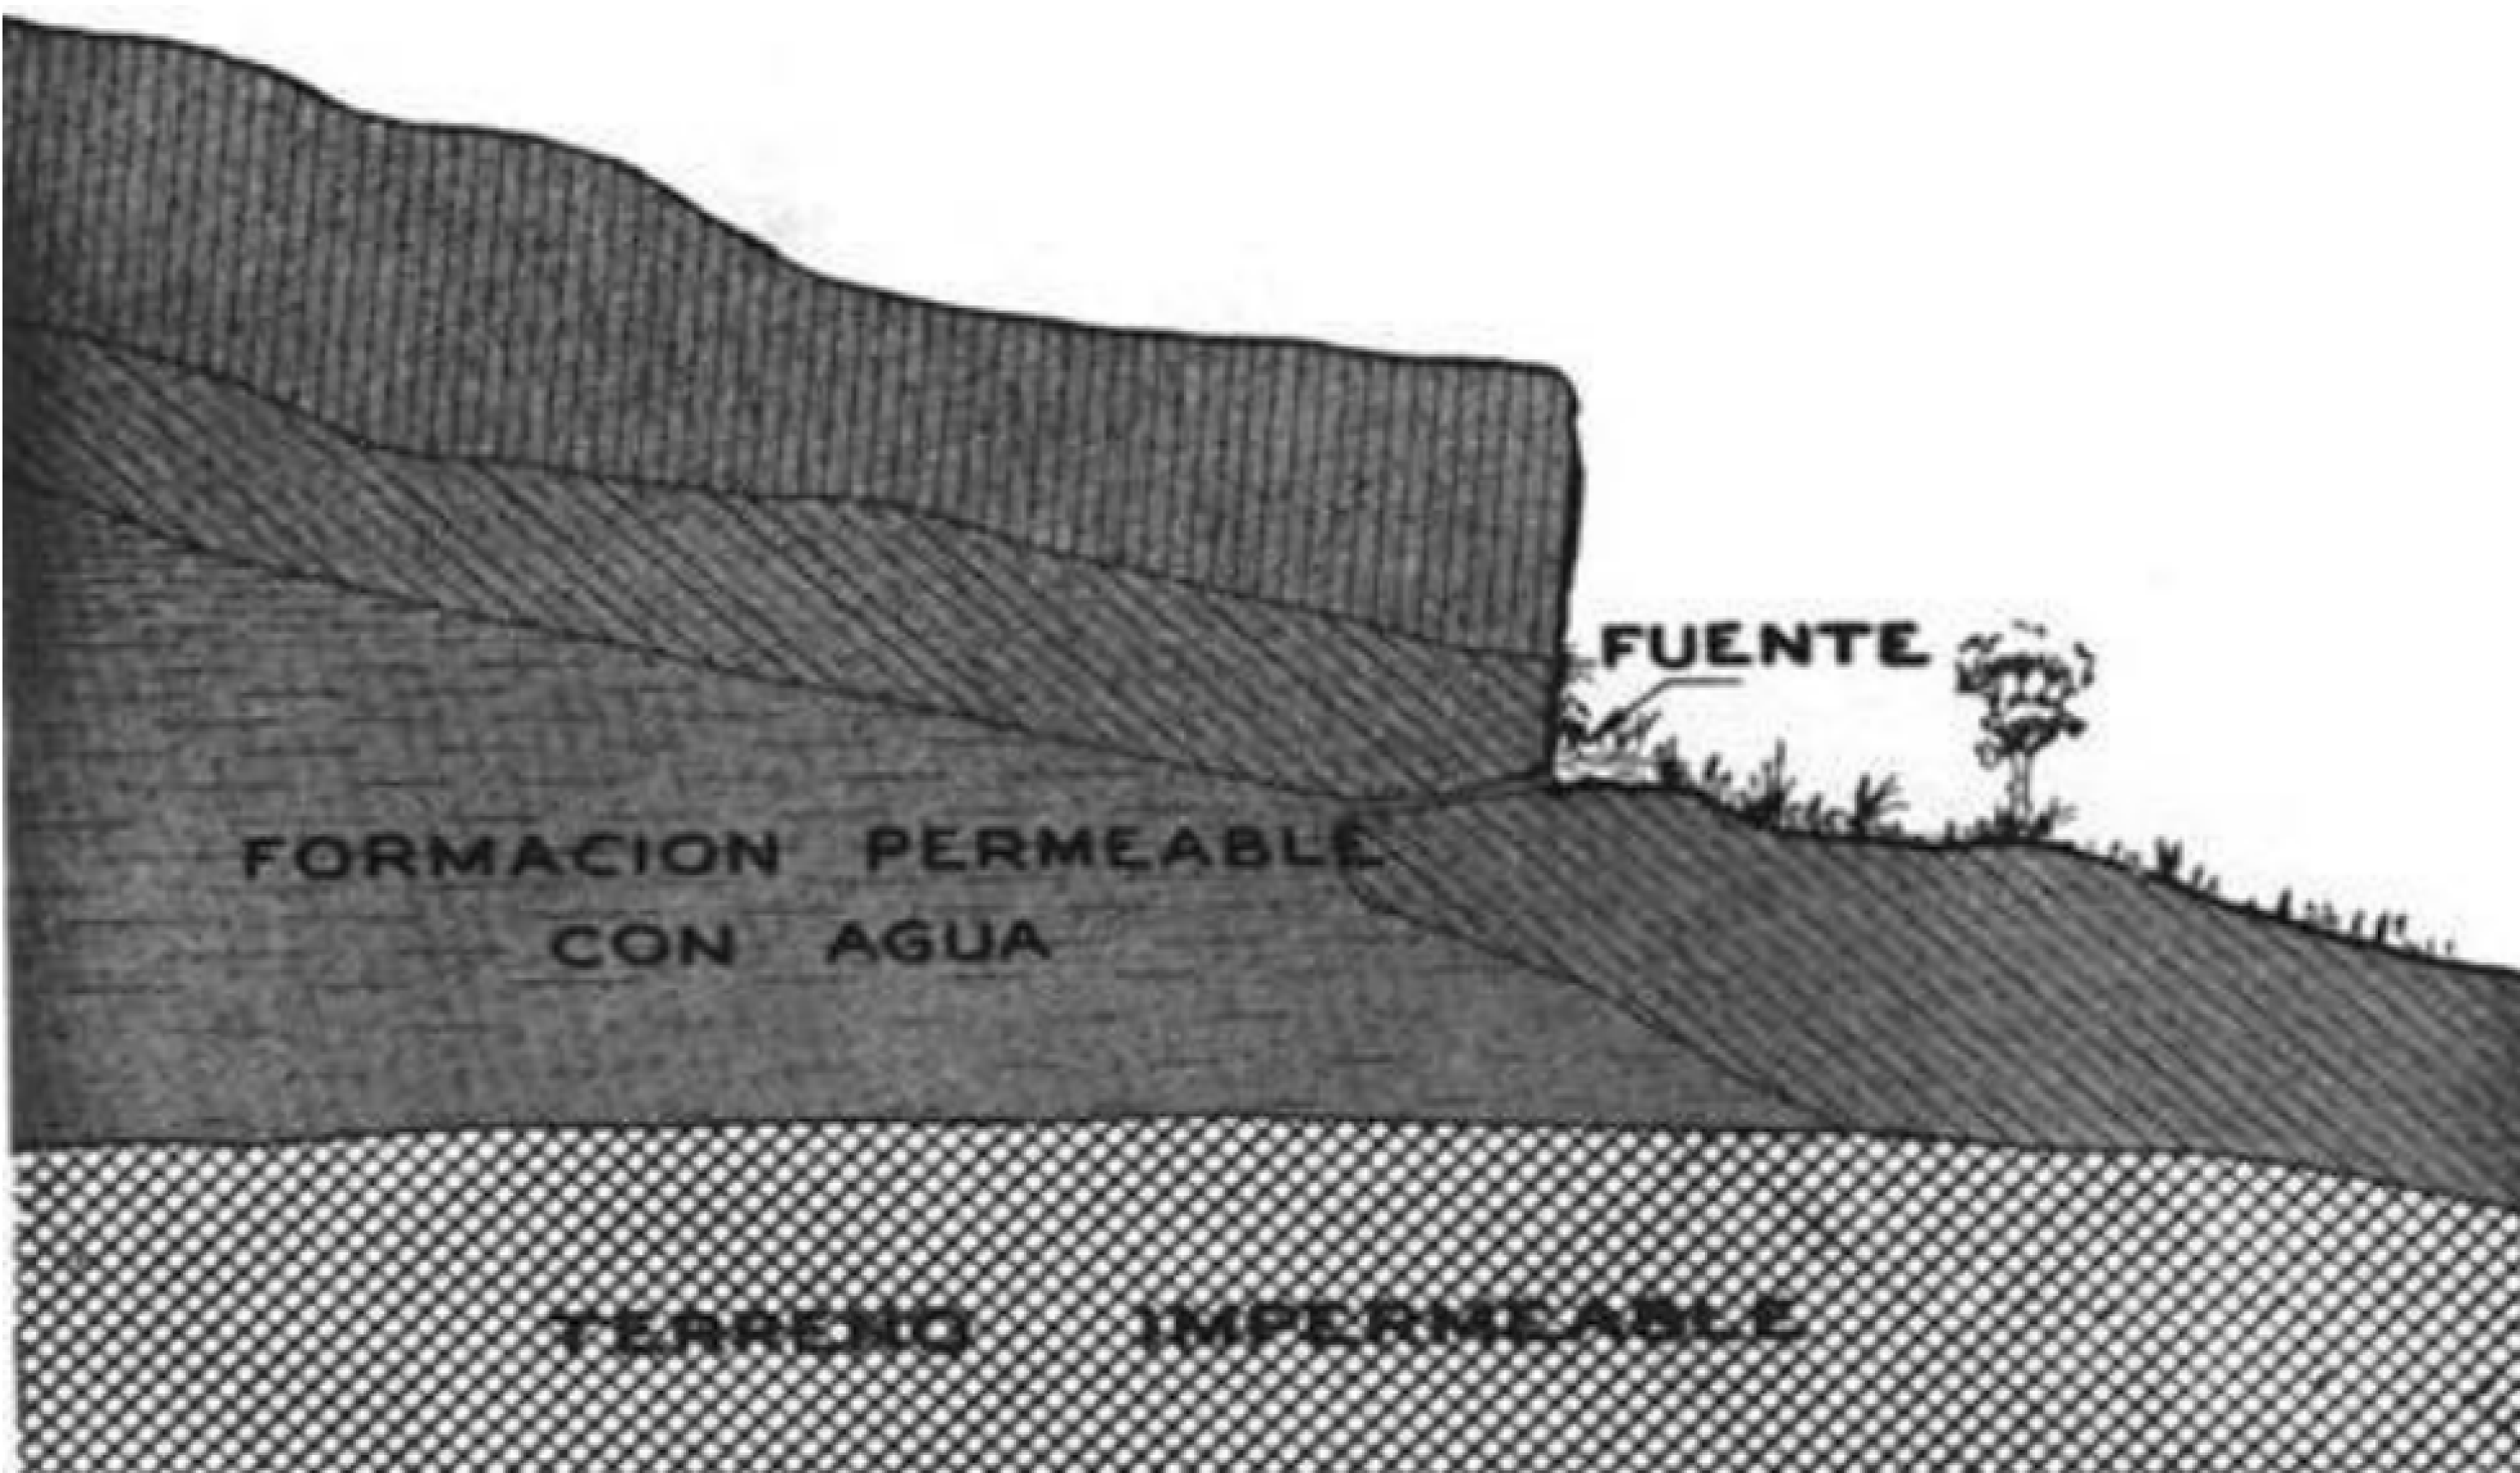
\includegraphics[width=\linewidth]{fii9.png}
		\caption{Manantial de afloramiento, en el que el agua mana como consecuencia
			de la carga a que está sometido, a través de una discontinuidad de la capa
			impermeable.}
		\label{fii9}
	\end{subfigure}
	\begin{subfigure}[b]{0.4\linewidth}
		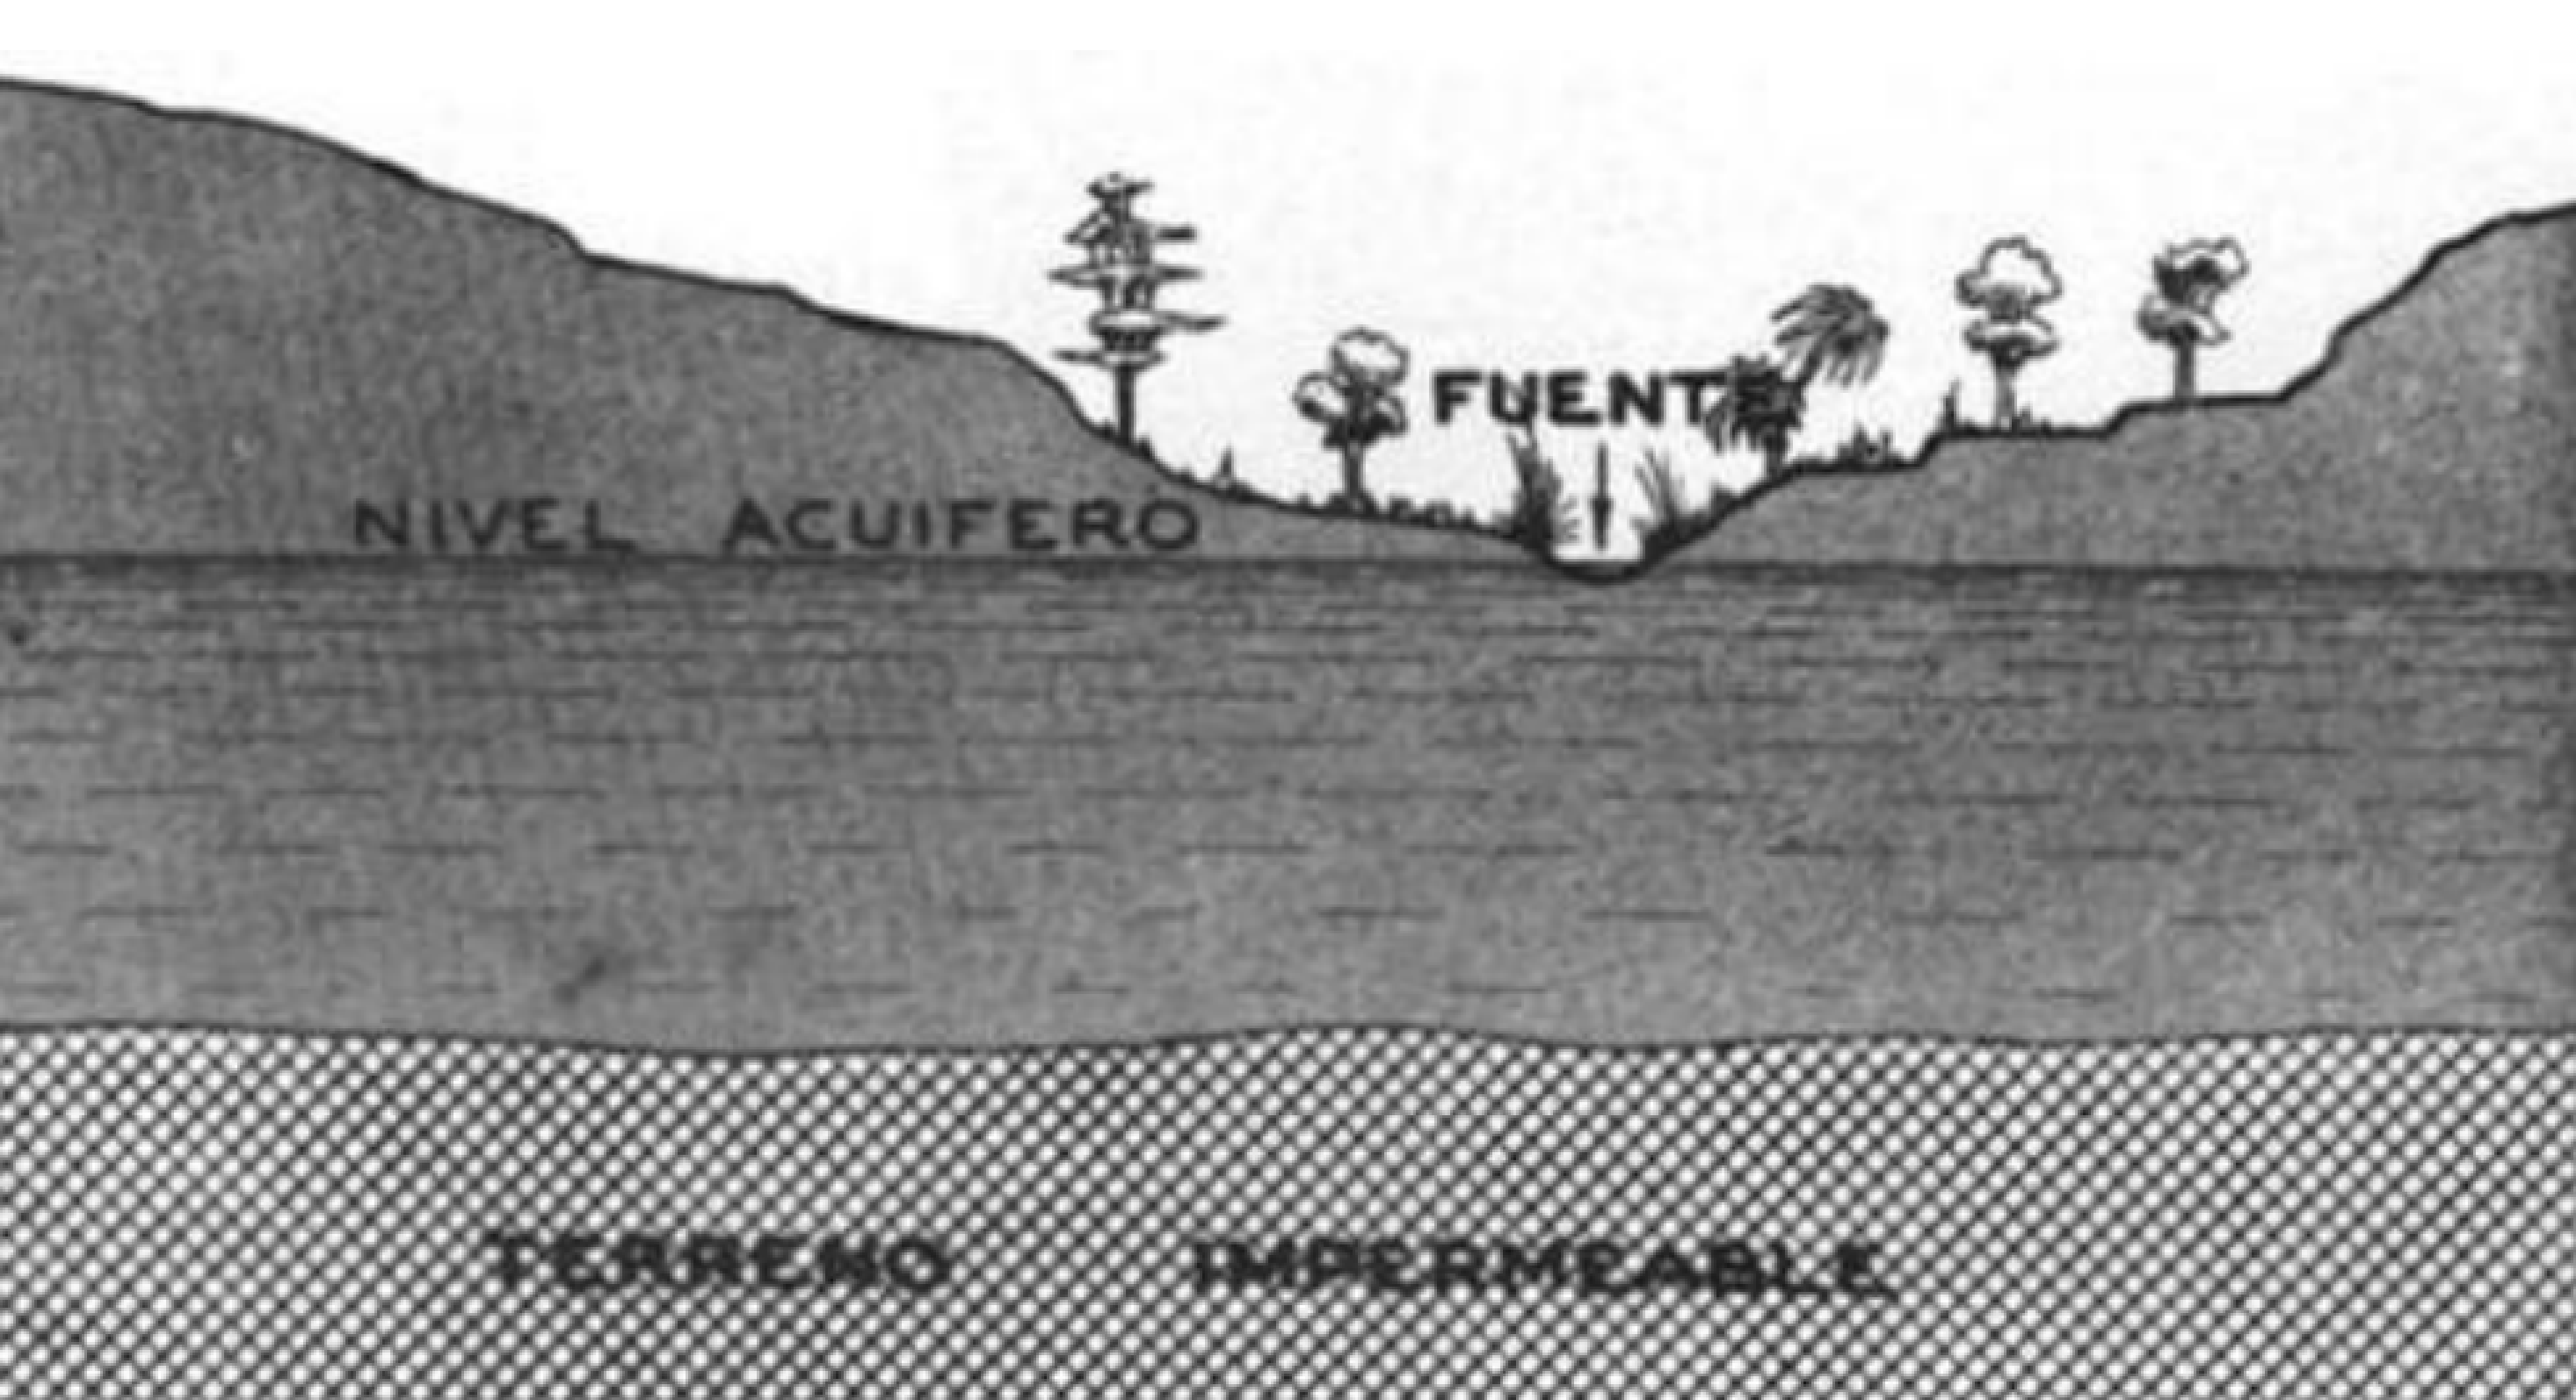
\includegraphics[width=\linewidth]{fii10.png}
		\caption{ Manantial de vaguada, debido a la existencia de una depresión del
			terreno por debajo del nivel del acuífero.}
		\label{fii10}
	\end{subfigure}
	\caption{Manantiales o fuentes}
	\begin{subfigure}[b]{0.4\linewidth}
		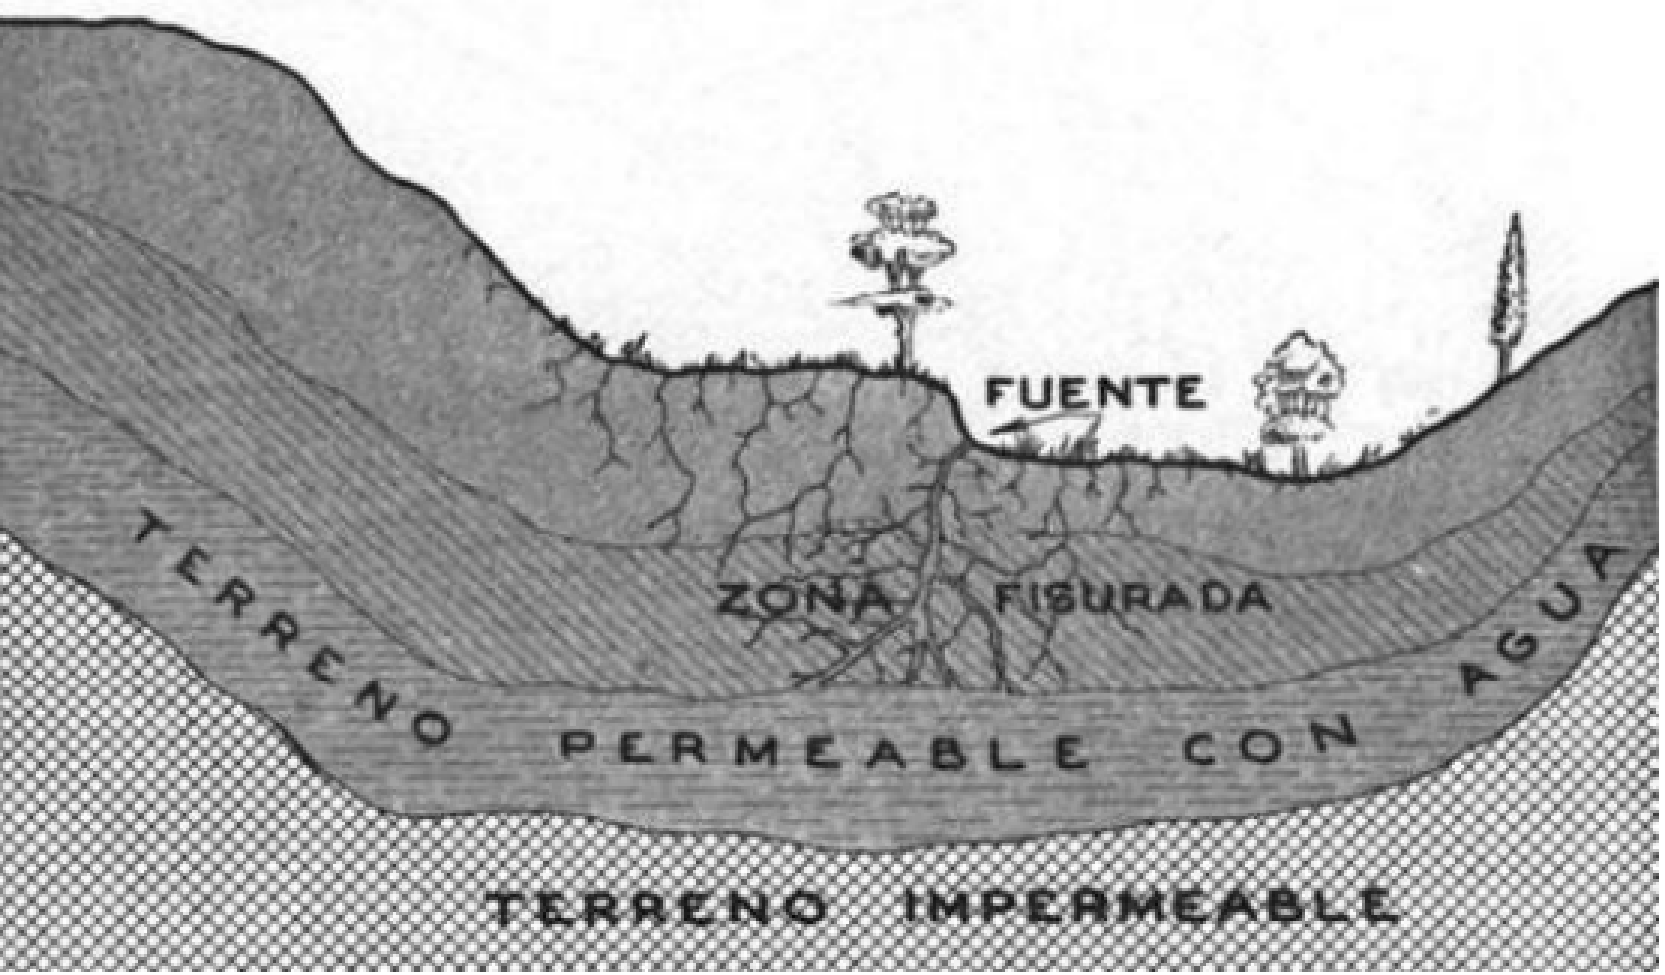
\includegraphics[width=\linewidth]{fii11.png}
		\caption{Manantial de grieta o de filón, el cual mana a través de una
			formación fisurada y cuyas aguas proceden de un manto profundo, a veces
			termal.}
		\label{fii11}
	\end{subfigure}
	\begin{subfigure}[b]{0.4\linewidth}
		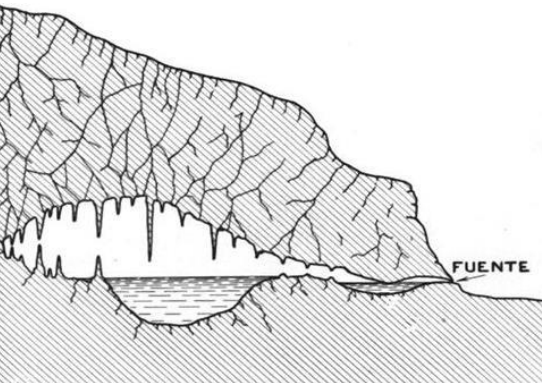
\includegraphics[width=\linewidth]{fii12.png}
		\caption{ Manantial intermitente, el cual cesa de manar cuando alcanza cierta
			altura el agua en el depósito subterráneo que lo alimenta.}
		\label{fii12}
	\end{subfigure}
	\caption{Manantiales o fuentes}
	\label{fig9-12}
\end{figure}

\begin{figure}
	\centerline{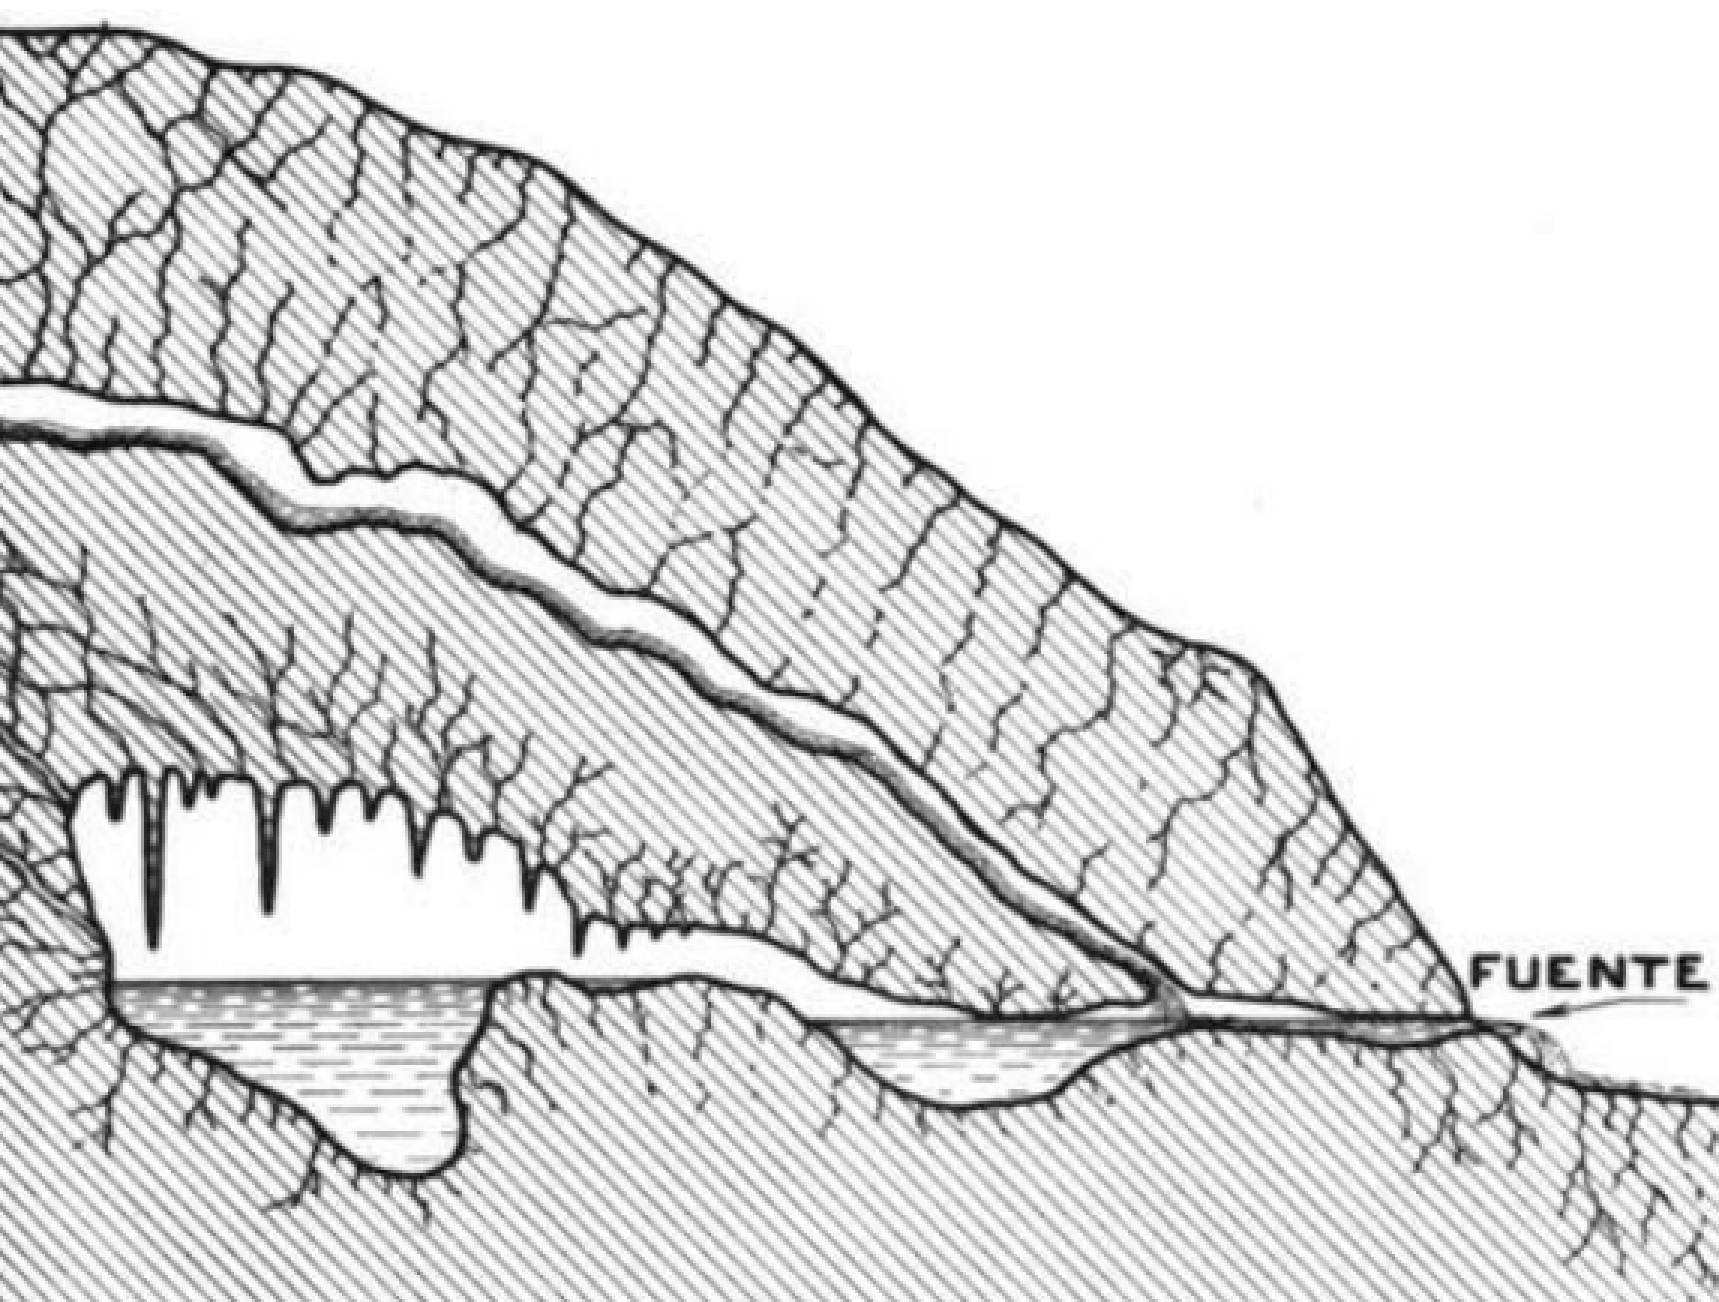
\includegraphics[width=0.5\textwidth]{fii13.png}}
	\caption{manantial intercalar, que ofrece variaciones de gastos por la
		coexistencia de un depósito de intermitencia y de una alimentación continua.}
	\label{fii13}
\end{figure}

existen tres tipos de diámetros en los \textbf{pozos}, véase la figura \ref{fig14-17}:
\begin{enumerate}
	\item Pequeño diámetro: Diámetros de perforación de 5 a 60 cm de forma circular.
	\item De gran diámetro: Diámetros de excavación de 1 a 5 m en formas circular, rectangular y
	      elíptica
	\item   Mixtos: Pozo de pequeño diámetro construido en uno de gran diámetro.
\end{enumerate}


\begin{figure}[h!]
	\centering
	\begin{subfigure}[b]{0.45\linewidth}
		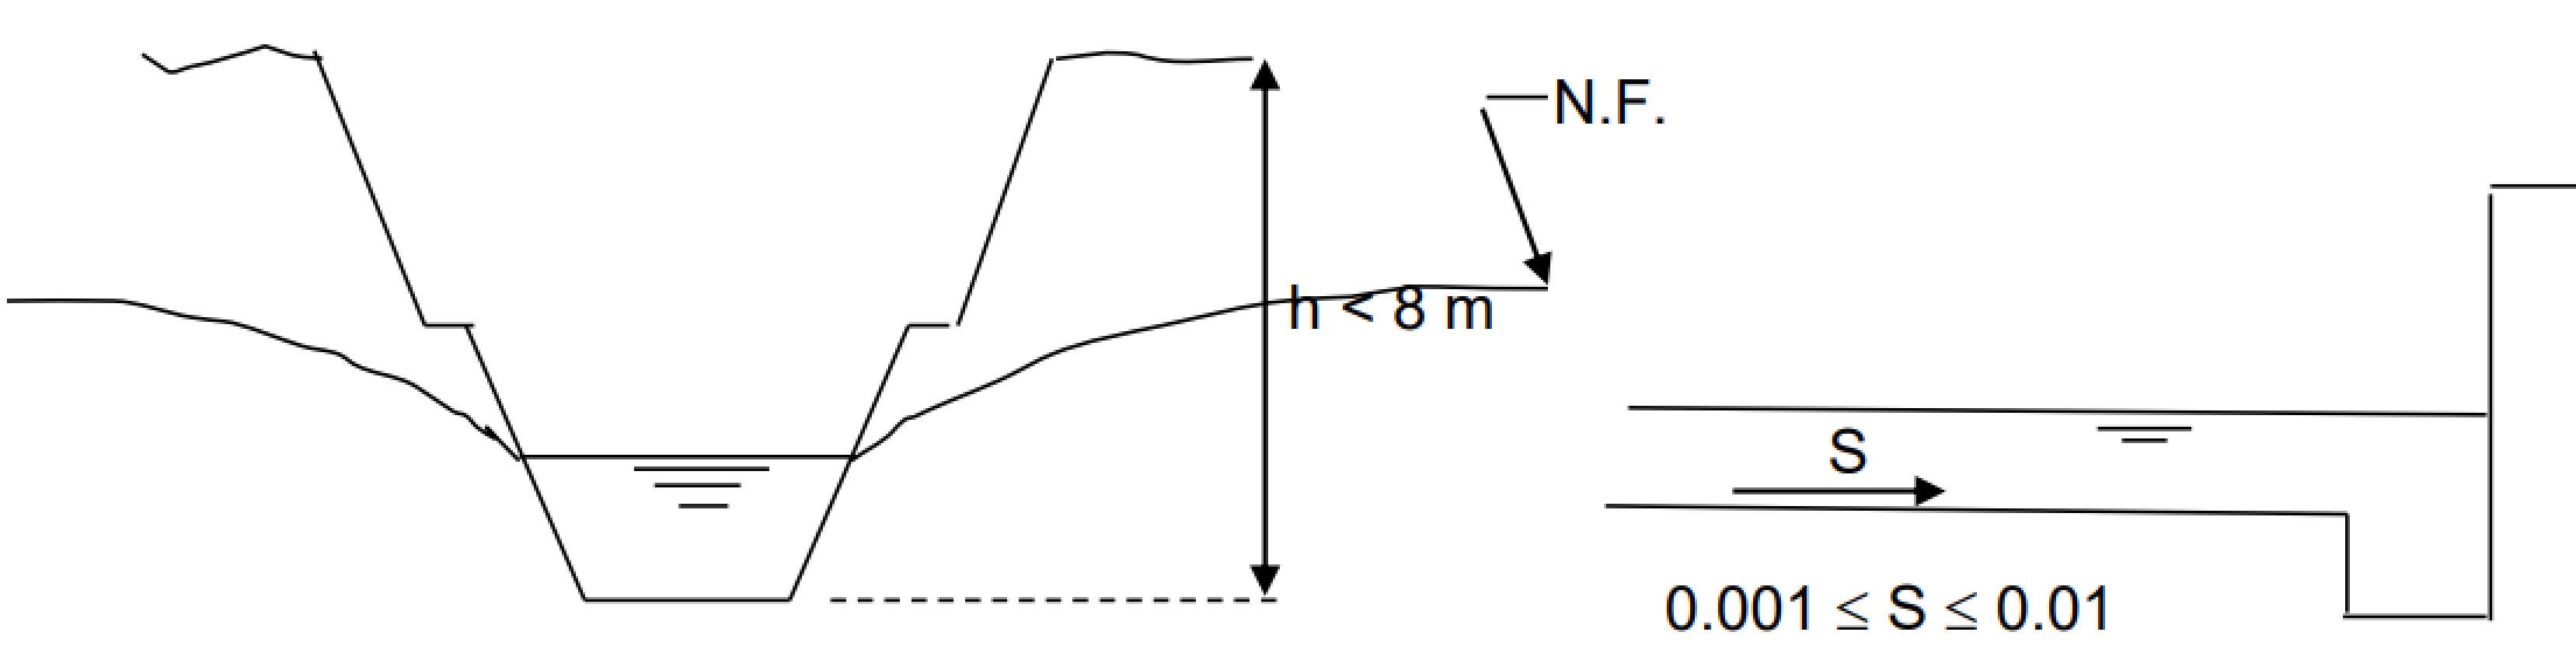
\includegraphics[width=\linewidth]{fii14.png}
		\caption{Trincheras colectoras}
		\label{fii14}
	\end{subfigure}
	\begin{subfigure}[b]{0.3\linewidth}
		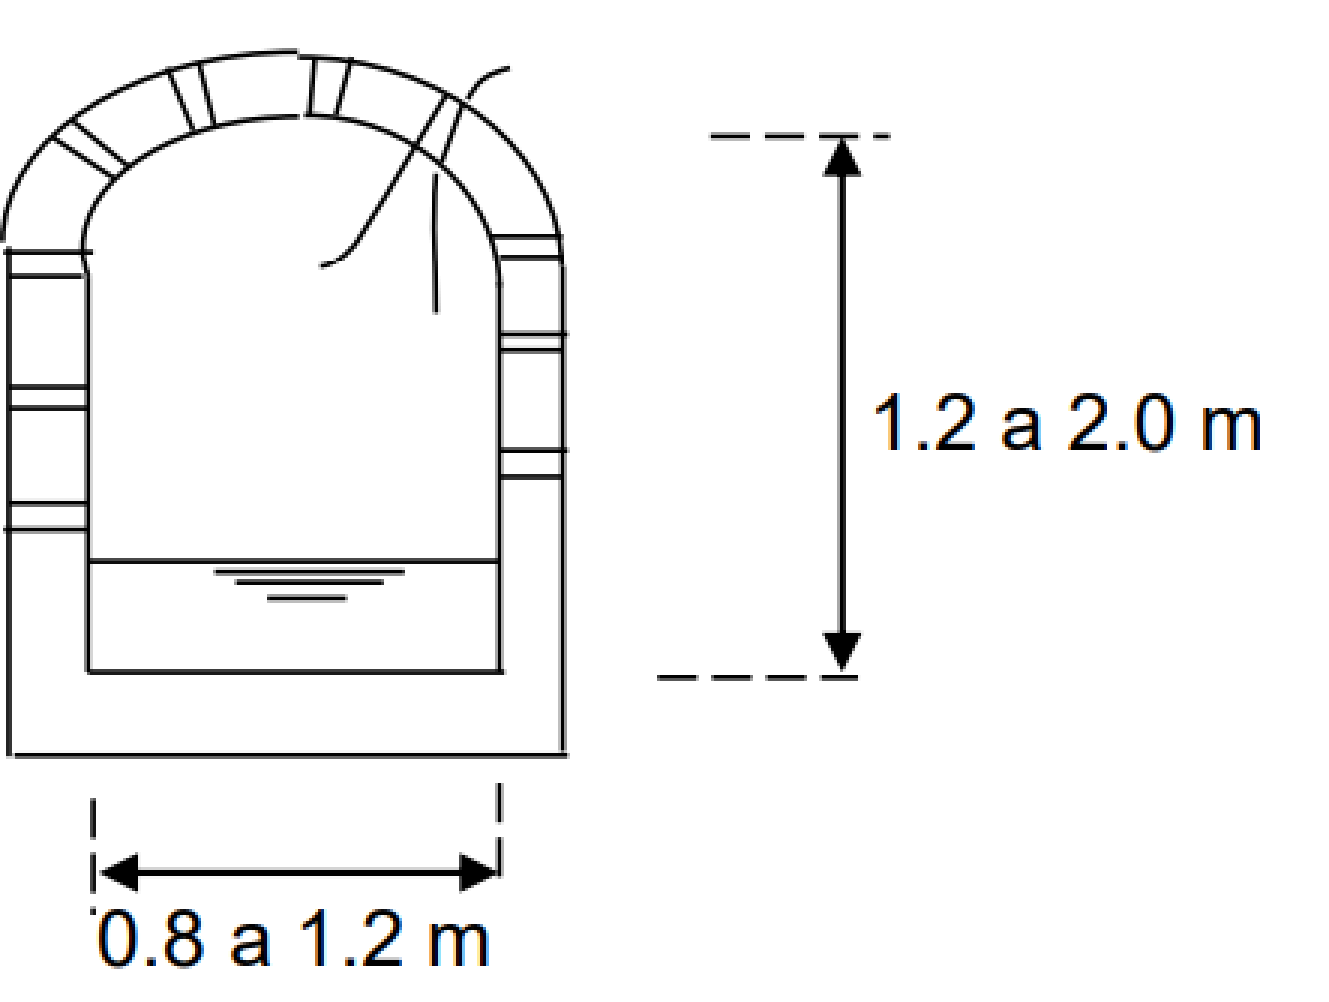
\includegraphics[width=\linewidth]{fii15.png}
		\caption{Galerías Filtrantes}
		\label{fii15}
	\end{subfigure}
	\begin{subfigure}[b]{0.45\linewidth}
		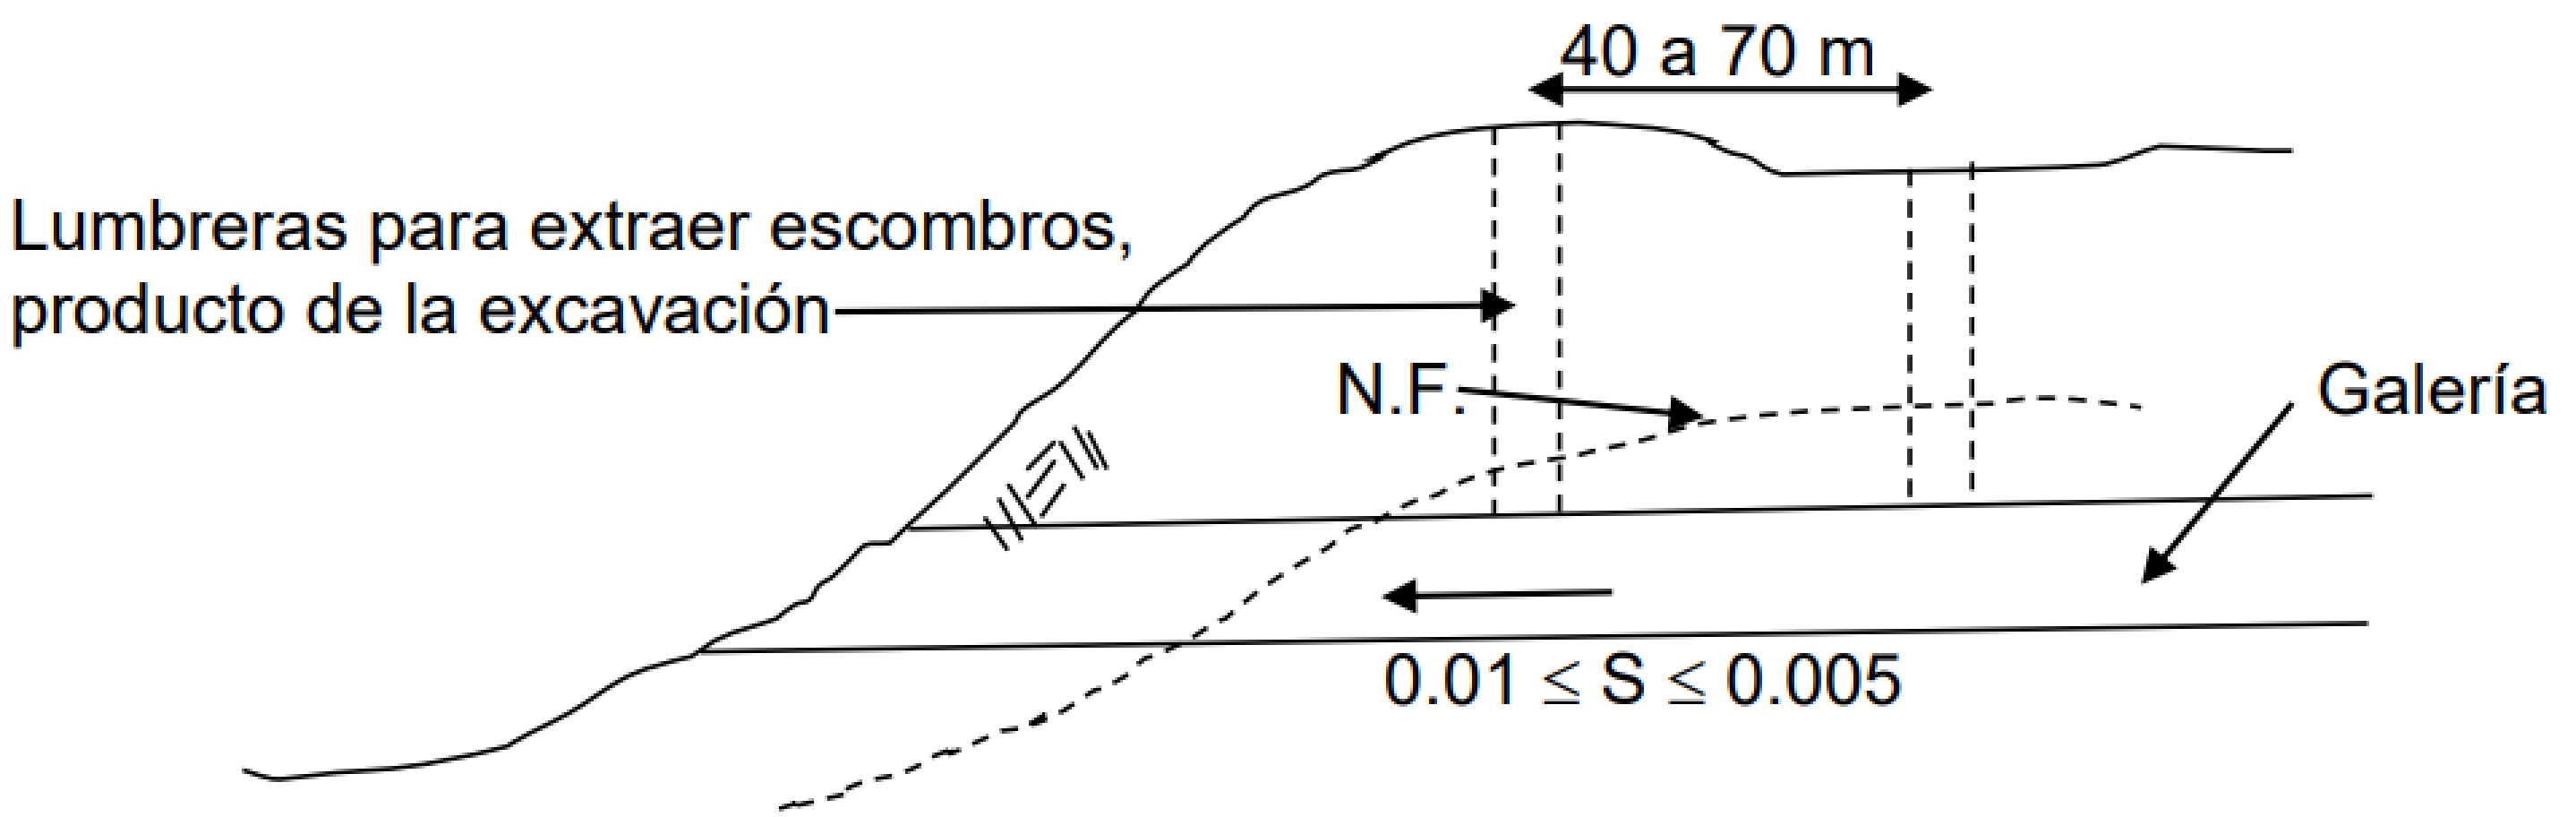
\includegraphics[width=\linewidth]{fii16.png}
		\caption{Galerías de Captación}
		\label{fii16}
	\end{subfigure}
	\begin{subfigure}[b]{0.45\linewidth}
		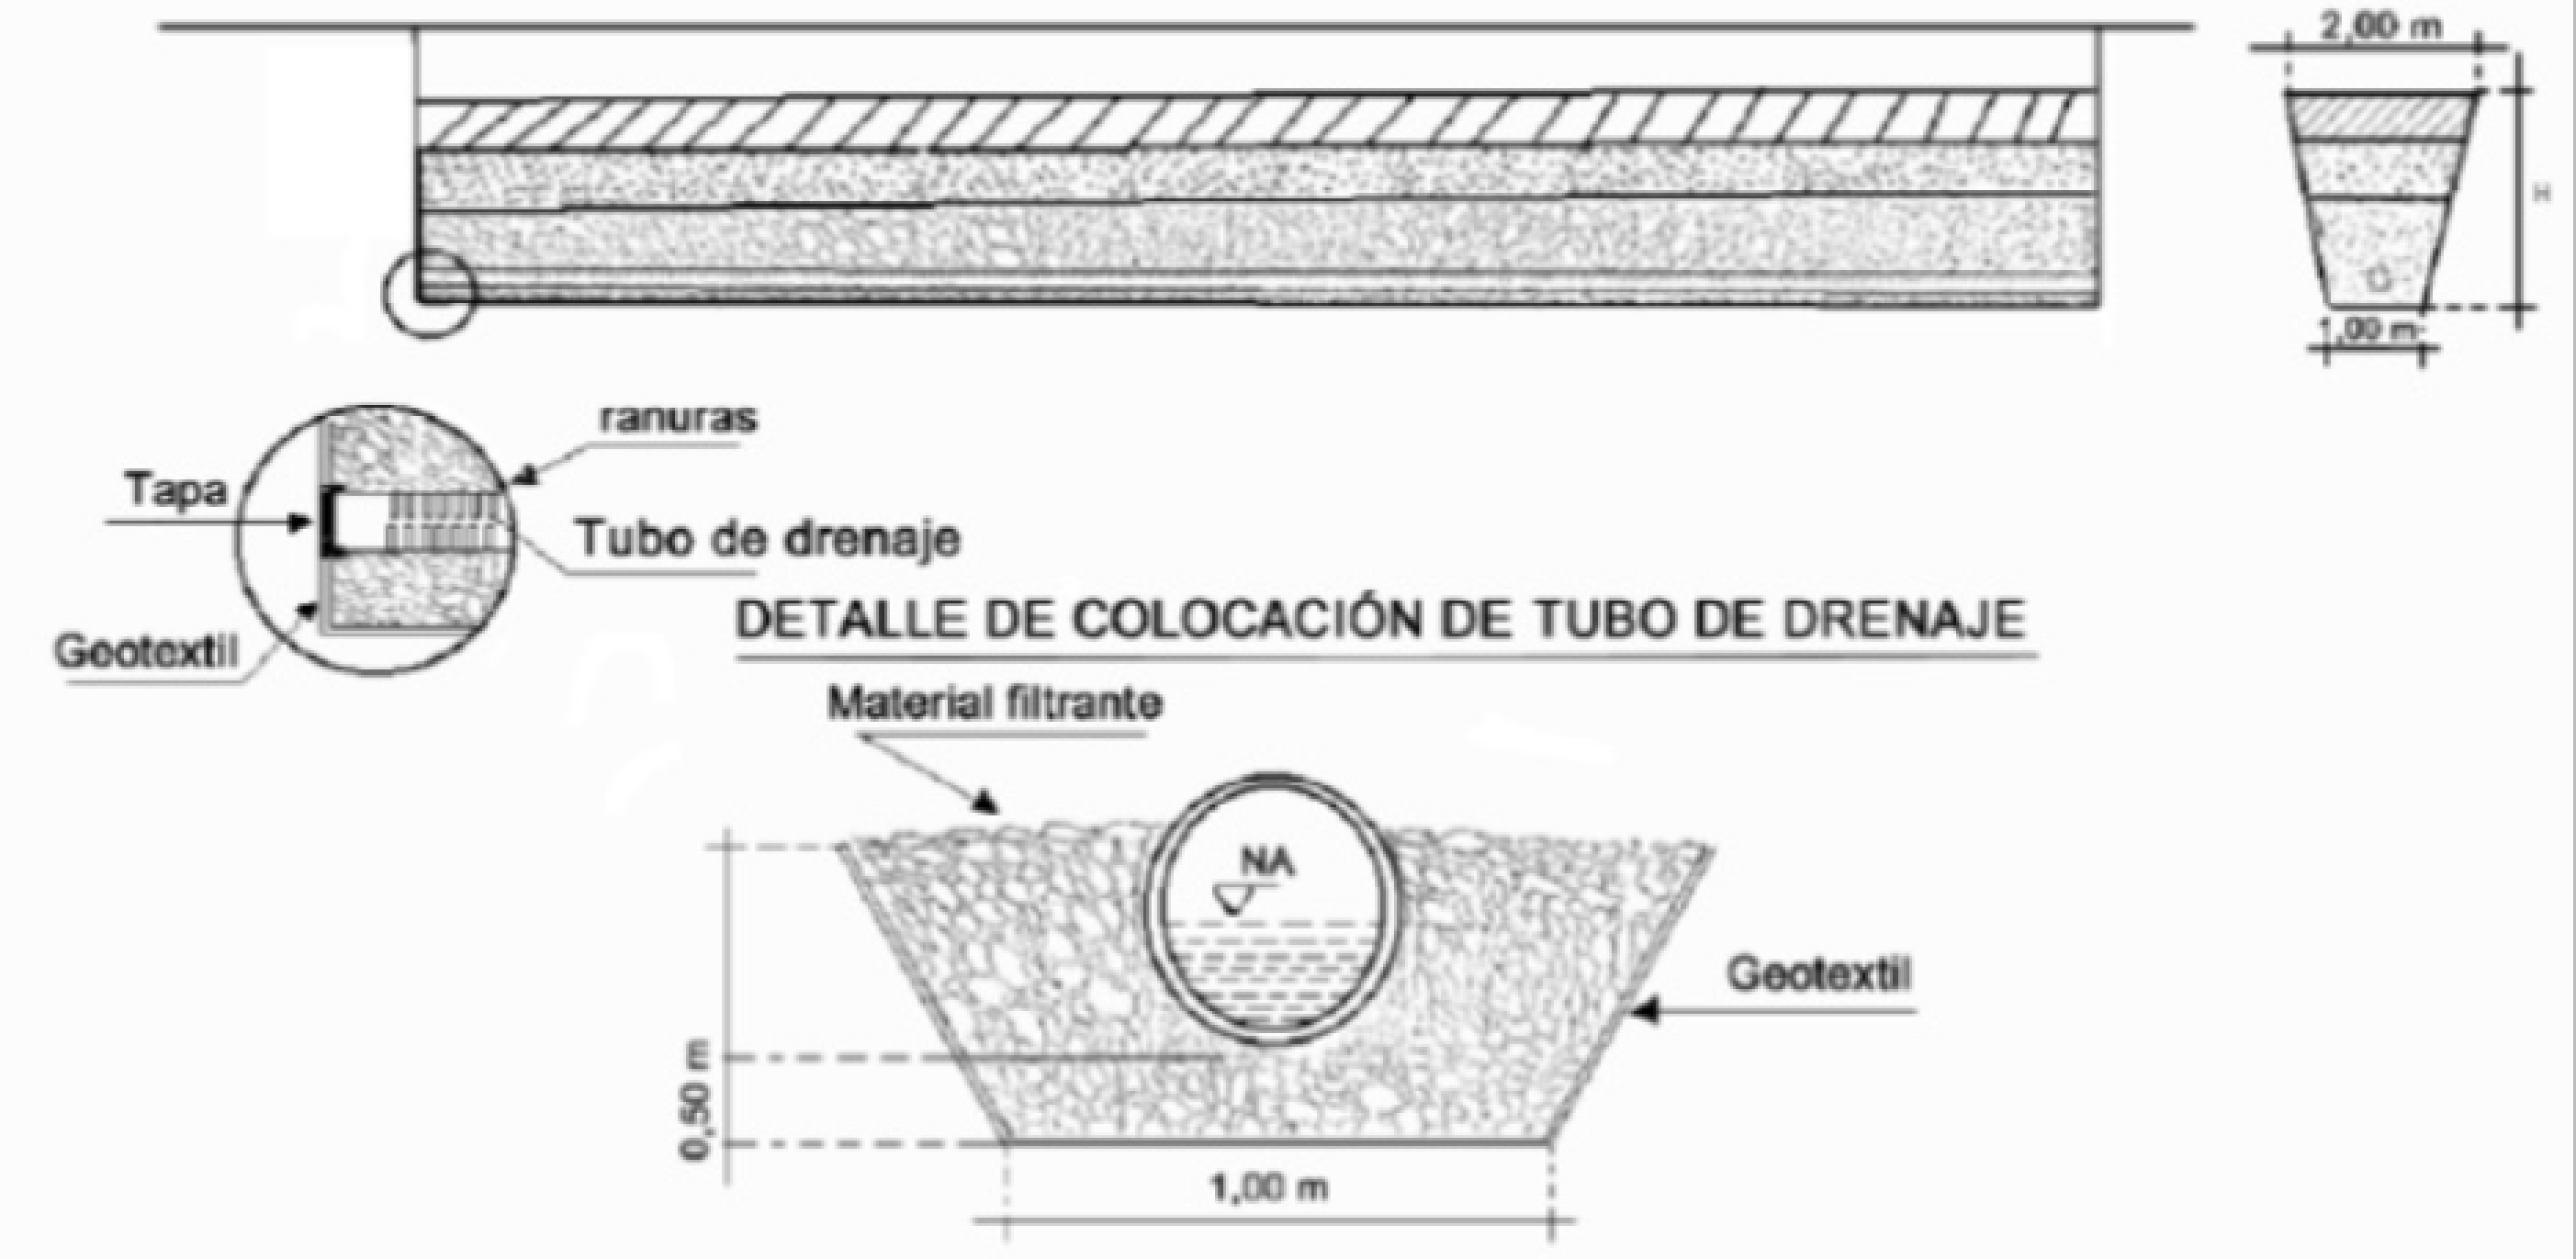
\includegraphics[width=\linewidth]{fii17.png}
		\caption{Galerías en el Fondo de Pozos}
		\label{fii17}
	\end{subfigure}
	\caption{Pozos}
	\label{fig14-17}
\end{figure}

Sí la galería es de longitud considerable, se requieren lumbreras o pozos para
extraer escombros, a distancias no mayores de 50 o 60 m.
Ventajas e inconvenientes de la explotación de Acuíferos.

Ventajas:
\begin{itemize}
	\item  Menores pérdidas por evaporación con relación a los aprovechamientos de
	      aguas superficiales
	\item Menor exposición a la contaminación
	\item Disponibilidades de agua menos afectadas por las variaciones climáticas
	\item No existe pérdida en la capacidad de almacenamiento
	\item Temperatura del agua constante.
\end{itemize}

Desventajas:
\begin{itemize}
	\item  Alto costo, tanto de construcción como de operación
	\item Aguas con riesgo de afectación salina
	\item Abatimientos acelerados de los acuíferos
	\item Para fines agrícolas, los gastos disponibles son de 20 a 65 lps (bombas entre
	      4" y 8" de diámetro en turbinas verticales)
	\item Se presentan grandes dificultades en la operación, por los pequeños gastos
\end{itemize}

Factores que afectan la explotación de las aguas subterráneas, al utilizar bombeo
\begin{itemize}
	\item Aspecto legal
	\item Rendimiento del pozo
	\item Niveles de abatimiento
	\item Éxito de empresas locales semejantes
	\item Disponibilidad de energía y/o combustibles
	\item Estudio agroeconómico y diseño ingenieril
	\item Posibilidades de recarga natural o artificial.
\end{itemize}

\subsubsection{Balance hidrológico de la cuenca}
Dependiendo del origen que se tenga del agua, según el FOGAFAGA \autocite{de1958fomento}, esta
puede ser clasificada como:

\begin{enumerate}
	\item \textbf{Agua meteórica}. Esta agua se deriva de la atmósfera, se precipita en la
	      superficie y puede penetrar en las reservas del subsuelo y regresar de nuevo a la
	      atmósfera.
	\item \textbf{Agua juvenil}. Esta es agua nueva, que de acuerdo a cuál es su origen a su vez
	      se subclasifica en: magmática, volcánica y cósmica. El agua juvenil magmática, es el
	      agua desalojada del magma durante su cristalización; el agua juvenil volcánica, es el
	      agua que proporciona los escurrimientos de lava; y el agua juvenil cósmica es el agua
	      que proviene del espacio con los meteoritos.
	\item \textbf{Agua rejuvenecida}. Es el agua que regresa o se une de nuevo al agua terrestre
	      por procesos geológicos de compactación y metamorfismo. La compactación reduce la
	      porosidad de sedimentos arcillosos desde un 50\% en material depositado
	      recientemente hasta 3 o 4\% en lutitas. Este tipo de agua rejuvenecida se puede
	      denominar aguas de compactación.
	\item \textbf{Agua connata}. Esta agua es aquella que se presenta como bolsas de agua
	      estancada, especialmente en estructuras que contienen aceite y gas.
	      Las principales reservas naturales del agua son: la atmósfera, la cual abastece a
	      todas las demás reservas; la superficie del suelo sobre la cual se encuentra el agua en
	      corrientes, lagos, océanos y agua sólida como nieve y hielo; la zona del suelo, la cual
	      actúa como reserva de humedad del suelo útil a la vida vegetal y la reserva de aguas
	      subterráneas.
\end{enumerate}

El agua es un constituyente variable de la atmósfera cuya cantidad varía con la
temperatura del aire. Grandes cantidades de vapor de agua están presentes en el aire
caliente saturado de los trópicos. El agua está limitada en la atmósfera en la zona de
convección, ese decir el estrato basal de la atmósfera de once kilómetros de espesor.
La lluvia es la fuente de toda el agua superficial y subterránea y por lo tanto debe ser
medida y analizada.

El agua superficial consta de dos cuerpos distintos de agua en la naturaleza: a)
el agua oceánica, la cual se encuentra altamente mineralizada. El cuerpo de
agua oceánica contiene agua para cubrir todo el globo terráqueo; es la principal fuente
de humedad atmosférica y por ende, de los demás cuerpos de agua. b) Los cuerpos
superficiales de agua dulce, que cubren pequeñas porciones de la superficie terrestre.
El agua dulce se halla en ríos, depósitos y lagos; es almacenada durante el invierno
como nieve o hielo.

Aún en regiones caracterizadas por abundantes cuerpos de agua superficial, la
mayoría de seres vivos, no vivirían si el agua almacenada del
suelo no fuera útil para la conservación de las plantas. Tomando como promedio 1.5 m
de espesor de la zona que penetran las raíces, la humedad contenida en el suelo es
equivalente a poco menos de 30 cm de agua. El agua almacenada en el suelo está
adherida a las partículas del mismo y es removida en gran parte por la transpiración de
las plantas. Este déficit o pérdida debe ser repuesto antes de que el agua se pueda
mover hacia abajo, hasta el espejo del agua a través de la zona vacía del suelo. Por
consiguiente, la filtración del agua de lluvia no puede ser una fuente importante del
agua en regiones áridas.

\subsubsection*{Agua para fines agrícolas.}
En forma natural, se tiene en la precipitación, la cual
para satisfacer las necesidades de la planta, se debe contar con un
temporal eficiente, de lo contrario, se recurre a
fuentes secundarias de agua, ya sea de agua superficial o de agua subterránea.
En México, como se señaló en la sección \ref{subsubciclohidro}, se tiene una precipitación promedio
de 780 mm. El escurrimiento superficial se estima del orden del 27\% de la
precipitación, haciendo un total de 410,000 millones de $ m^3$ como escurrimiento virgen, y
357,565 millones de $ m^3$ como escurrimiento disponible para aprovecharse, con una
distribución un tanto similar a como se presenta la precipitación. véase la figura \ref{fii8}.

Por su naturaleza, la cuantificación del agua subterránea permite identificar:
31,000 millones de $m^3$ de agua subterránea renovable anualmente y 110,000 millones
de $ m^3$ de agua subterránea no renovable.

\begin{figure}[h!]
	\centerline{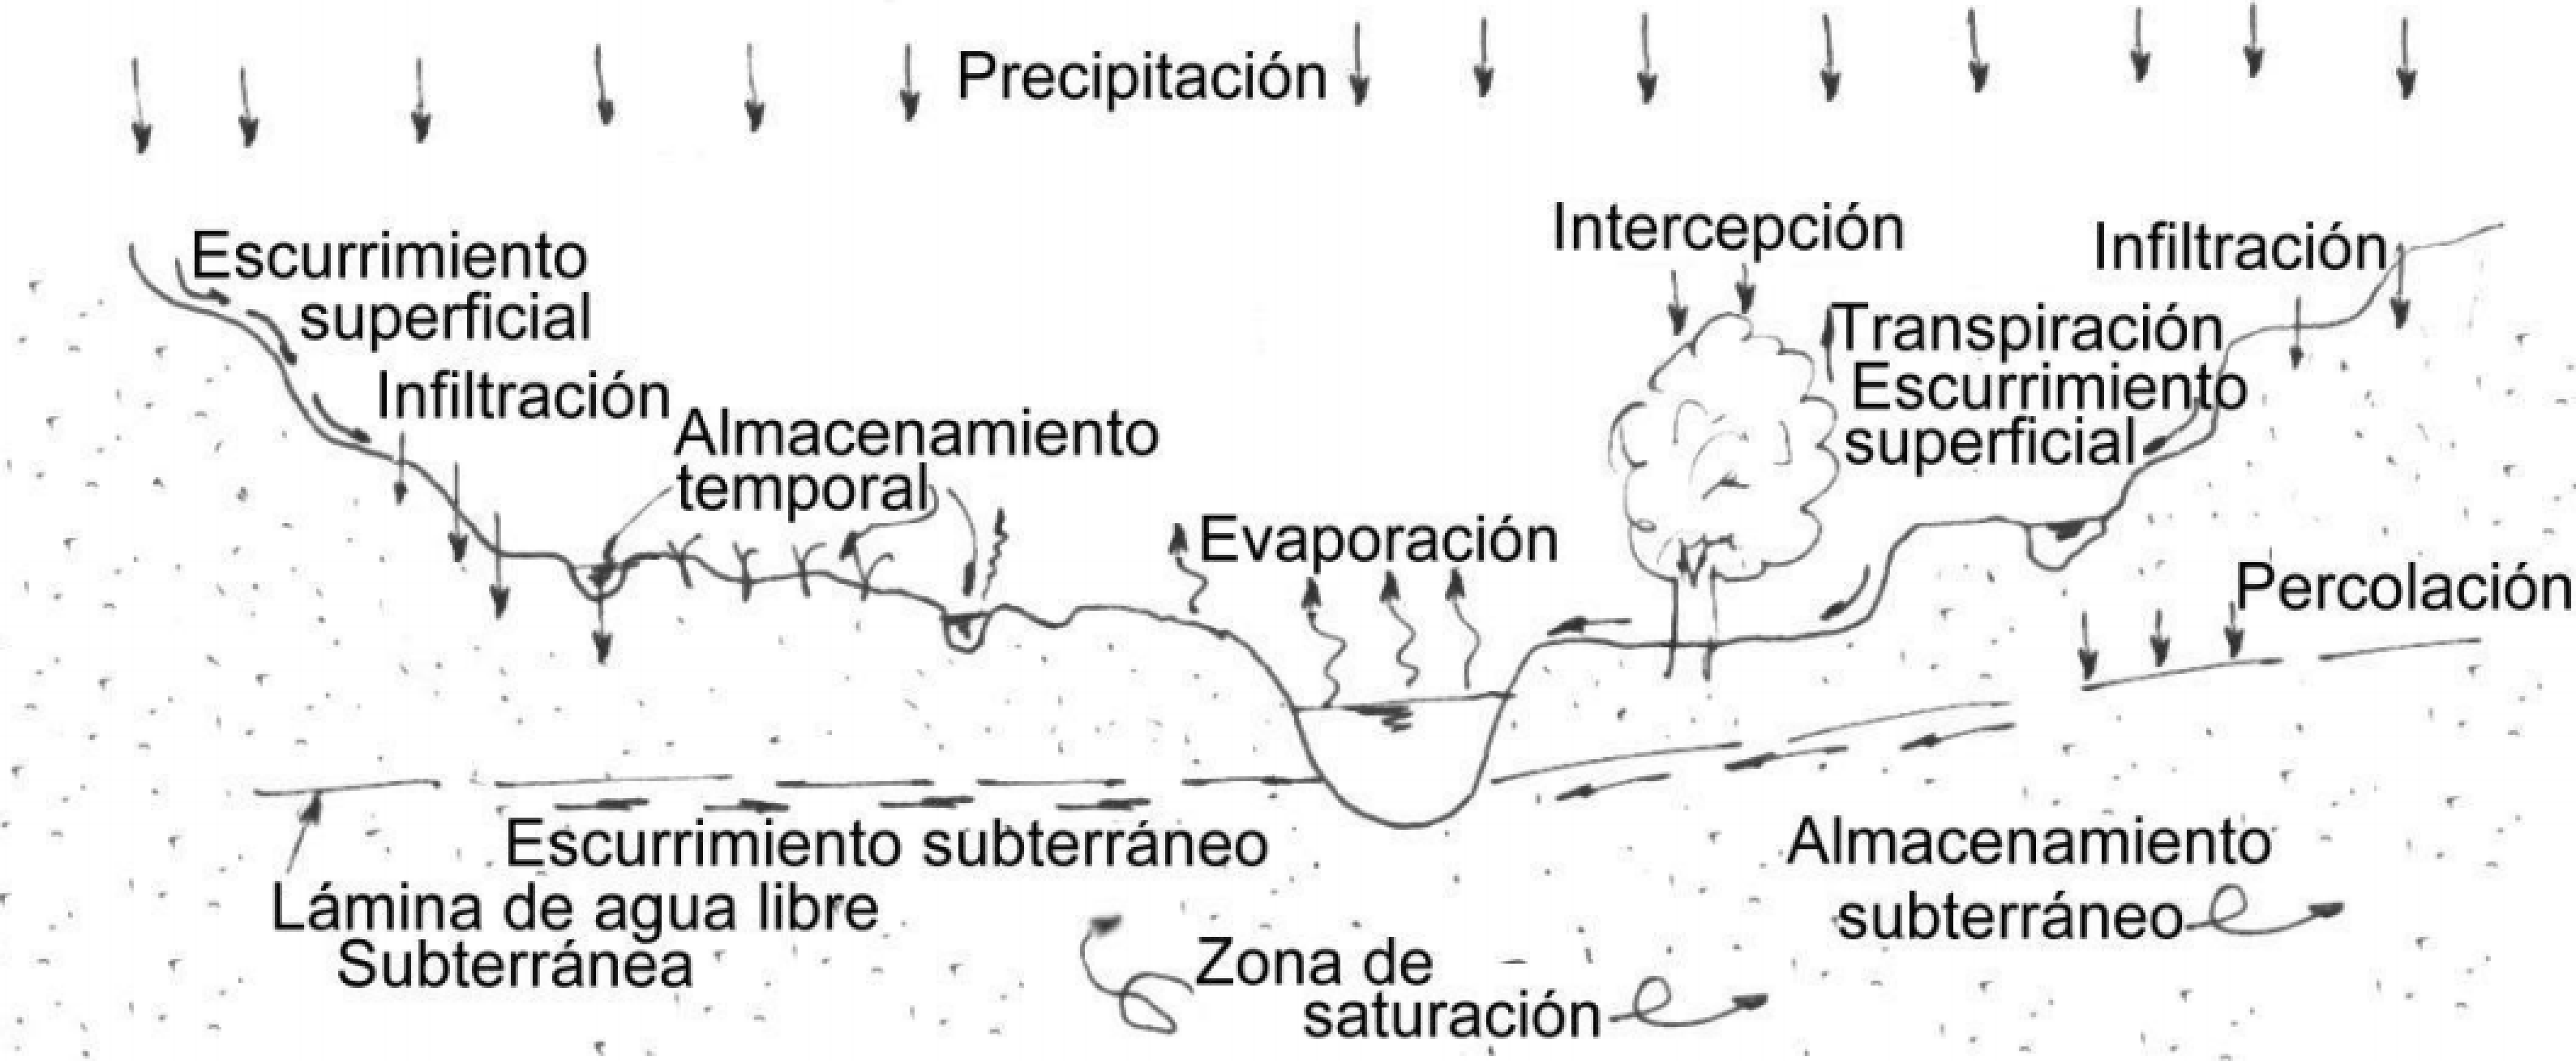
\includegraphics[width=0.7\textwidth]{fii18.png}}
	\caption{Disposición de la humedad durante una lluvia intensa (según Houk)}
	\label{fii18}
\end{figure}

\subsubsection{Ciclo del agua}
Las principales fuentes de energía para la circulación del agua en la naturaleza
son: el sol y la gravedad.
\begin{definition}[Evaporación]
	Según su definición hidrológica es la tasa neta de
	transporte de vapor hacia la atmósfera.
	La tasa de evaporación varía según la naturaleza de la superficie evaporante y
	de diversos factores meteorológicos. En la primera, están todas las superficies
	expuestas a la precipitación tales como vegetales, edificios, calles pavimentadas, que
	vienen a representar superficies potenciales de evaporación; entre los segundos se
	tiene como principal factor a la radiación y en forma secundaria, a la velocidad del
	viento y la presión de vapor de la capa de aire inmediatamente superior.
\end{definition}

\begin{definition}[Precipitación]
	Es el agua que llega a la superficie terrestre proveniente de la
	atmósfera. Este es un componente fundamental del ciclo hidrológico.
	Las formas de precipitación, se tienen dependiendo de las condiciones
	meteorológicas existentes, pudiendo ser:
\end{definition}
\begin{itemize}
	\item \textbf{llovizna}: gotas de agua con diámetro
	      menor de 0.5 mm y su intensidad es generalmente de 1.0mm/h por lo cual semejan
	      estar flotando en el aire y por ello siguen con facilidad el curso del viento
	\item \textbf{Lluvia}: son
	      gotas de agua que caen de las nubes con un diámetro superior a 0.5 mm y a
	      velocidades que varían de acuerdo a su intensidad y puede a su vez dividirse en lluvia
	      ligera (2.5 mm), mediana o moderada (2.5 a 7.5 mm) o intensa o fuerte (diámetros de
	      7.5 mm), si la lluvia y llovizna se presentan cuando la temperatura ambiente es menor a
	      0$^{\circ}$C entonces se forma una capa de hielo en las superficie en que caen
\end{itemize}

\begin{definition}[Granizo]
	Está constituido por bolas o pedriscos de hielo de 5 a 50 mm que son producto de la
	condensación de gotas de lluvia formando granos de hielo duro, poco transparente y de
	forma globular, que caen separados o en grupos irregulares
\end{definition}

\begin{definition}[Nieve]
	La constituyen
	cristales de hielo de color blanco, traslucido ramificado, generalmente en forma de
	estrellas hexagonales (vistos al microscopio). Atendiendo a su intensidad, esta puede
	ser ligera, moderada y fuerte y la nieve puede observarse sola o acompañada de algún
	otro fenómeno que disminuye la visibilidad.
\end{definition}

\begin{definition}[Rocío]
	Es el vapor de agua que se
	condensa sobre la superficie a causa de que el aire ambiente sufre un descenso de
	temperatura, este descenso nunca es inferior a 0$^{\circ}$C
\end{definition}

\begin{definition}[Escarcha]
	Es debida a un
	fenómeno llamado de sublimación, por el cual los cristales de hielo son formados
	directamente sobre las superficies, en virtud de que el aire se ha enfriado a menos de
	0$^{\circ}$C.
\end{definition}

La precipitación puede ser: \textbf{convectiva}, \textbf{ciclónica} u \textbf{orográfica}.

\begin{definition}[Precipitación convectiva]
	Se origina por el calentamiento del suelo, que
	provoca corrientes ascendentes de aire húmedo. La precipitación asociada a este tipo
	de fenómeno afecta áreas reducidas, del orden de 25 a 50 $Km^2 $, y su intensidad varía
	entre lloviznas ligeras y aguaceros, dependiendo de las condiciones de temperatura y
	humedad.
\end{definition}

\begin{definition}[precipitación ciclónica]
	Está asociada al paso de ciclones, resulta del
	levantamiento de aire por convergencia de la masa de aire en una zona de baja
	presión. En general afectan zonas extensas. Se divide en dos tipos: frontal y por
	convergencia.
\end{definition}

\begin{definition}[Precipitación ciclónica frontal]
	Puede ser de frente caliente o de frente frío,
	siendo originada por el levantamiento de aire caliente sobre el frío, y puede ocurrir
	cuando el aire caliente se mueve hacia el frío (frente caliente) o viceversa (frente frío).
	La precipitación provocada por un frente caliente se distribuye sobre un área bastante
	grande y varía entre intensidades ligeras y moderadas. La precipitación de frente frío es
	de intensidades fuertes y de corta duración.
\end{definition}

\begin{definition}[Precipitación ciclónica por convergencia]
	Es causada por la tendencia del aire
	húmedo a converger hacia el centro del ciclón. El aire al no poder concentrarse en un
	área menor tiende a elevarse, por lo cual se enfría provocando la precipitación.
	La precipitación orográfica es consecuencia del ascenso del aire producido por
	las barreras montañosas; su distribución en el espacio está relacionada con las
	pendientes del terreno.
\end{definition}

En terrenos demasiado abruptos, la influencia orográfica es muy
señalada, por lo que la distribución espacial de las lluvias tiende a parecerse de una
tormenta a otra. Cuando no está relacionada con acciones ciclónicas o convectivas,
resulta ser de baja intensidad tal como se muestra en la figura \ref{fii19}.

\begin{figure}[h!]
	\centerline{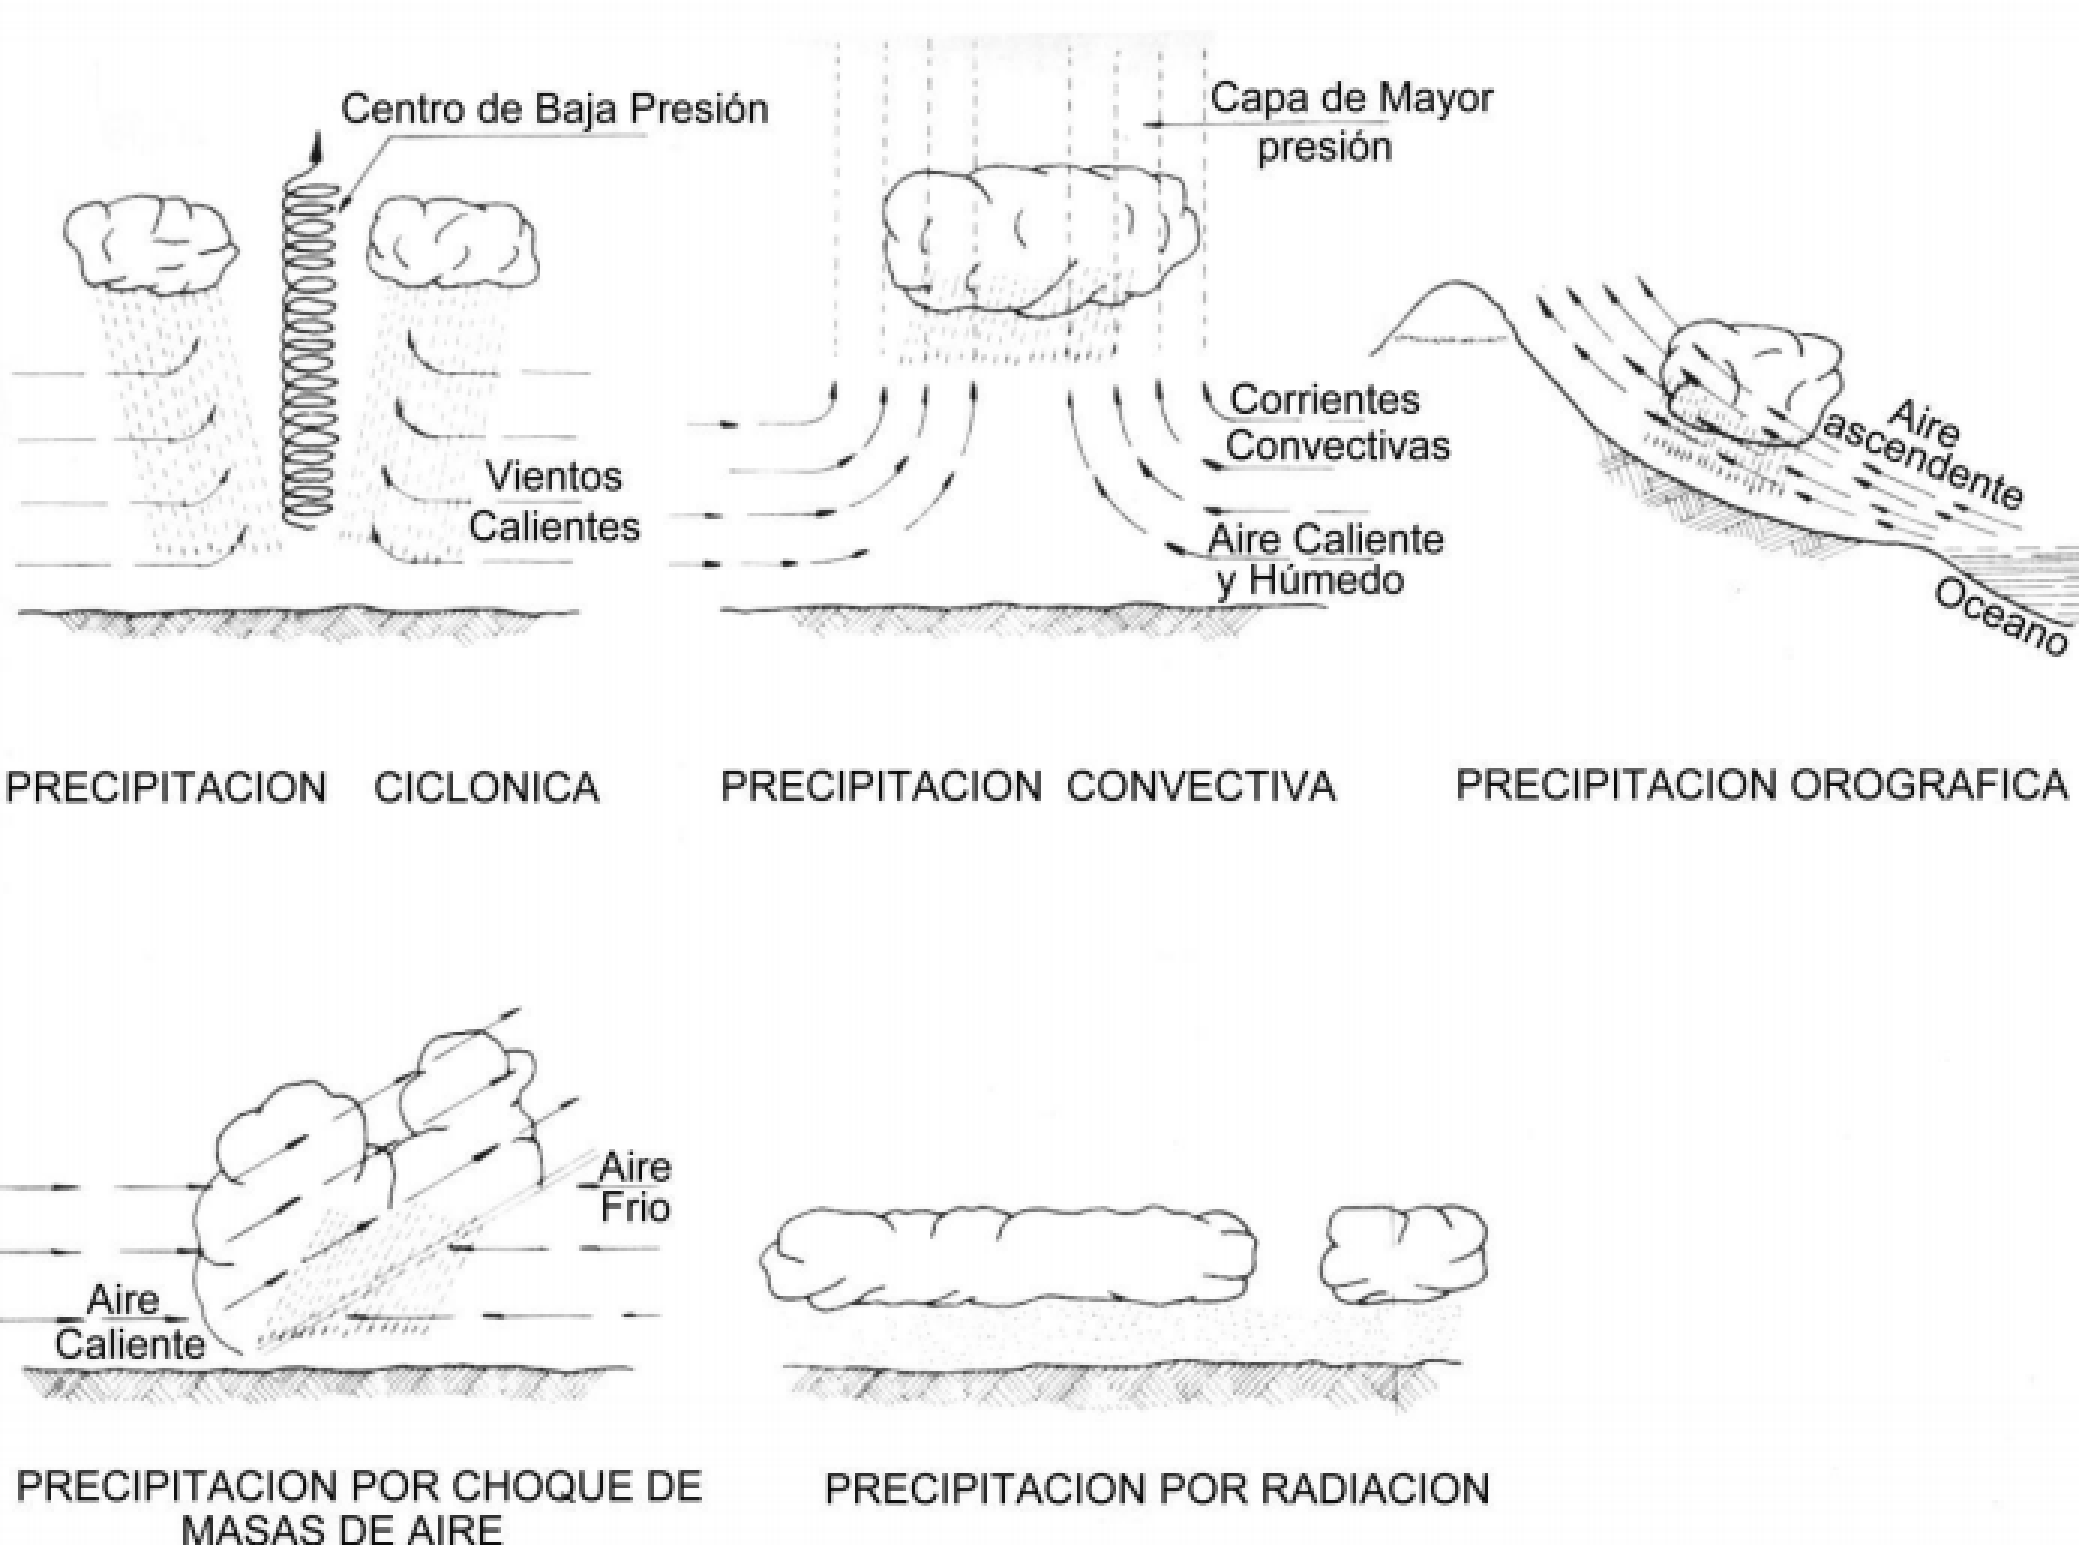
\includegraphics[width=0.7\textwidth]{fii19.png}}
	\caption{Esquemas de los tipos de precipitación}
	\label{fii19}
\end{figure}

\subsubsection{Distribución de la precipitación.}

\textbf{Infiltración}. Es el movimiento vertical del agua, a través de las capas
superficiales del suelo, producido por la acción de las fuerzas gravitacionales y
capilares.

Esta es la porción más considerable de las pérdidas de la precipitación. Existen
diferentes métodos para calcular la infiltración, entre las que se pueden citar la de
Horton y la de Kostiakov.

\textbf{Evaporación}. Existe otra porción de la precipitación que se pierde cuando
va cayendo y esta es la evaporación que se tiene cuando caen las gotas de agua.

\textbf{Transpiración}. Es el agua que se despide en forma de vapor de las hojas
de las plantas. Esta agua es tomada por las plantas en forma natural del suelo.

\textbf{Almacenamiento temporal}. En las depresiones del terreno, se presenta
una retención por determinado tiempo de cierta cantidad de agua, la que después parte
se infiltra y parte se evapora.

\textbf{Escurrimiento}. Es el agua proveniente de la precipitación que circula
sobre o bajo la capa superficial del suelo o en estratos más profundos y que llega a una
corriente para finalmente ser drenada hasta la salida de una cuenca. Existen tres tipos
de escurrimiento: superficial, subsuperficial y subterráneo.

La relación entre el volumen escurrido y el volumen precipitado en una
determinada cuenca es lo que origina el concepto de \textbf{coeficiente de escurrimiento} $(Ce)$,
fundamental para determinar el primero conociendo el segundo, variando entre valores
que van de $0.1$ a $0.25$.

\subsubsection{Los consejos de cuenca}
Los Consejos de Cuenca son instancias de coordinación y concertación entre la
Comisión Nacional del Agua, las dependencias y entidades de las instancias federal, estatal,
municipal y los representantes de los usuarios de la respectiva cuenca hidrológica: Su objeto es
formular y ejecutar programas y acciones para la mejor administración de las aguas, el
desarrollo de la infraestructura hidráulica y de los servicios respectivos y la preservación de los
recursos de la cuenca (Art. 13, LAN).

Para su funcionamiento, los Consejos de Cuenca pueden contar con organizaciones
auxiliares a nivel de subcuenca, microcuenca y/o acuífero, denominadas respectivamente:
Comisiones de Cuenca, Comités de Cuenca y Comités Técnicos de Aguas Subterráneas
(Cotas).

%imágen aquí vaaaaaaaaaaaaaaaaaaaaaaaaaaa

Al año 2000, se tenían instalados 25 consejos de cuenca, así mismo al año 2003
se tenían instaladas 11 comisiones de cuenca y al año 2004, 16 comités de cuenca y
69 Comités Técnicos de Aguas Subterráneas (COTAS).

\subsection{Ley de Aguas Nacionales.}

La ley de aguas nacionales es reglamentaria de artículo 27 de la Constitución
política de los Estados Unidos Mexicanos es de observancia general en todo el territorio
nacional, sus disposiciones son de orden público e interés social y tiene por objeto
regular la explotación, uso o aprovechamiento de dichas aguas, su distribución y
control, así como la preservación de su cantidad y calidad para lograr su desarrollo
integral sustentable.

Se conforma con 10 títulos, el título primero de \textbf{disposiciones generales} contiene
un solo capítulo y 3 artículos.

El Título Segundo, de la \textbf{Administración del agua}, contiene 10 capítulos y 11
artículos base y 20 sub articulos.

El Título Tercero, de la \textbf{política y programación hídrica}, contiene un solo capítulo,
pero dos secciones, un artículo y tres sub artículos.

El Título Cuarto, de los \textbf{Derechos de Explotación, Uso o Aprovechamiento de
	Aguas Nacionales}, contiene cinco capítulos y dos subcapítulos, 10 artículos y 8
sub artículos.

El Título Quinto, de las \textbf{Zonas Reglamentadas, de Veda o de Reserva}, contiene
un solo Capítulo, seis artículos y un subartículo.

El Título Sexto, de los \textbf{Usos del Agua}, con cinco capítulos y dos subcapítulos, el
capítulo dos tiene cinco secciones, y todos comprenden 41 artículos y siete
sub artículos.

El Título Séptimo, de la \textbf{Prevención y Control de la Contaminación de las Aguas y
	Responsabilidad por Daño Ambiental}, con dos capítulos, con 13 artículo y 10
sub artículos.

El Título Octavo, de la \textbf{Inversión en Infraestructura Hidráulica}, contiene cuatro
capítulos, 15 artículos y 3 sub artículos.

El Titulo Noveno, de los \textbf{Bienes Nacionales a Cargo de ``la Comisión''}, contiene
un solo capítulo, y 5 artículos y 4 sub artículos.

El Titulo Decimo, de las \textbf{Medidas de Apremio, Seguridad, Infracciones, Sanciones
	y Recursos}, contiene tres capítulos, 6 artículos y 6 sub artículos.

La anterior Ley es del año 1992, pero en el año 2003 se actualizó con 16
transitorios, en el año 2004, con un artículo, en el 2008 con un Transitorio, en el año
2011 se reforman y adicionan los artículos 7 Bis y 18 de la Ley, en el año 2011 con un
transitorio, en el año 2012 con un artículo y un transitorio.

Para poder implementar cualquier ley, se requiere del Reglamento, así el
Reglamento de la ley de Aguas Nacionales, el cual se conforma con 11 títulos:

El Título primero de las Disposiciones Preliminares, contiene un solo capítulo,
con 5 artículos.

El Título Segundo, de la Administración del Agua, contiene cuatro capítulos, con
15 artículos.

El Título Tercero, de la Programación Hidráulica, contiene un solo capítulo, con
seis artículos.

El Título Cuarto, de los Derechos de Uso o Aprovechamientos de Aguas
Nacionales, contiene cinco capítulos, con 44 artículos.

El Título Quinto, de las Zonas Reglamentadas, de Veda o de Reserva, contiene
un solo capítulo, con 8 artículos.

El Título Sexto, de los Usos del Agua, contiene cinco capítulos, el segundo
Capítulo tiene cinco secciones, que es el que se refiere al Uso Agrícola, y las secciones
son: la primera de Disposiciones generales, la segunda de Ejidos y comunidades, la
tercera de las Unidades de riego, la cuarta de los Distritos de Riego y la Quinta del
Drenaje Agrícola, todo el Título conforma 52 artículos.

El Título Séptimo, de la Prevención y Control de la Contaminación de las Aguas,
solo contiene un Capítulo, con 24 artículos.

El Titulo Octavo, de la Inversión en Infraestructura Hidráulica, contiene dos
capítulos, con 10 artículos.

El Titulo Noveno, de los Bienes Nacionales a Cargo de la Comisión, contiene un
solo capítulo, con 15 artículos.

El Titulo Décimo, de las Infracciones, Sanciones y Recursos, contiene tres
capítulos, con 16 artículos.

El Título Décimo Primero, de la Conciliación y Arbitraje, contiene un solo capítulo,
con cinco artículos.

El reglamento concluye con 14 Transitorios, para el año 1994. En el año 1997, se
reformó la ley de Aguas Nacionales con un solo artículo y dos transitorios; en el año
2002, se reforma el Artículo 13 del Reglamento, con un solo artículo y un transitorio.

\subsection{Cambio climático}
El estudio del clima es un campo de investigación complejo y en rápida evolución,
debido a la gran cantidad de factore que intervienen. El clima de la Tierra nunca ha
sido estático. Como consecuencia de alteraciones en el balance energético, está
sometido a variaciones en todas las escalas temporales, desde decenios a miles y
millones de años. Entre las variaciones climáticas más destacables que se han
producido a lo largo de la historia de la Tierra, figura el ciclo de unos 100,000 años, de
períodos glaciares, seguido de períodos interglaciares.

\begin{definition}[Cambio climático]
	Es la variación global del clima de la Tierra. Es debido
	a causas naturales y también a la acción del hombre y se producen a muy diversas
	escalas de tiempo y sobre todos los parámetros climáticos: temperatura,
	precipitaciones, nubosidad, etc$\dots$
\end{definition}

\begin{definition}[Efecto invernadero]
	Se refiere a la retención del calor del Sol en la atmósfera de la Tierra por parte de una capa de gases
	en la atmósfera. Sin ellos la vida, tal como la conocemos, no sería posible, ya que el
	planeta sería demasiado frío. Entre estos gases se encuentran el dióxido de carbono,
	el óxido nitroso y el metano, que son liberados por la industria, la agricultura y la
	combustión de combustibles fósiles. El mundo industrializado ha conseguido que la concentración de estos gases haya aumentado un 30\% desde el siglo pasado, cuando,
	sin la actuación humana, la naturaleza se encargaba de equilibrar las emisiones.
\end{definition}

Ya en el año 2001 el Tercer Informe de Evaluación del Grupo Intergubernamental
de Expertos sobre Cambio Climático \textbf{(IPCC)} ponía de manifiesto la evidencia
proporcionada por las observaciones de los sistemas físicos y biológicos que mostraba
que los cambios regionales en el clima, en concreto los aumentos de las temperaturas,
estaban afectando a los diferentes sistemas y en distintas partes del globo terráqueo.
Señalaba, en definitiva, que se están acumulando numerosas evidencias de la
existencia del cambio climático y de los impactos que de él se derivan. En promedio, la
temperatura ha aumentado aproximadamente $0{.}6^\circ C$ en el siglo XX. El nivel del mar ha
crecido de 10 a 12 centímetros y los investigadores consideran que esto se debe a la
expansión de océanos, cada vez más calientes.

El cambio climático nos afecta a todos. El impacto potencial es enorme, con
predicciones de falta de agua potable, grandes cambios en las condiciones para la
producción de alimentos y un aumento en los índices de mortalidad debido a
inundaciones, tormentas, sequías y olas de calor. En definitiva, el cambio climático no
es un fenómeno sólo ambiental sino de profundas consecuencias económicas y
sociales. Los países más pobres, que están peor preparados para enfrentar cambios
rápidos, serán los que sufrirán las peores consecuencias.

Se predice la extinción de animales y plantas, ya que los hábitats cambiarán tan
rápido que muchas especies no se podrán adaptar a tiempo. La Organización Mundial
de la Salud ha advertido que la salud de millones de personas podría verse amenazada
por el aumento de la malaria, la desnutrición y las enfermedades transmitidas por el
agua.

En consecuencia, aunque existen incertidumbres que no permiten cuantificar con
la suficiente precisión los cambios del clima previstos, la información validada hasta
ahora es suficiente para tomar medidas de forma inmediata, de acuerdo al denominado
``principio de precaución'' al que hace referencia el Artículo 3 de la Convención Marco
sobre Cambio Climático. La inercia, los retrasos y la irreversibilidad del sistema
climático son factores muy importantes a tener en cuenta y, cuanto más se tarde en
tomar esas medidas, los efectos del incremento de las concentraciones de los gases de
efecto invernadero serán menos reversibles.

\subsubsection{Consecuencias del cambio climático}
El cambio climático, desde la existencia de la tierra no solo ha permitido
modificar las condiciones de la naturaleza, sino que también va haciendo variaciones
en la economía; en la salud y en todas las poblaciones de una u otra manera.

No obstante, se ha determinado científicamente que el cambio climático va
llegando a su límite y al no ponerle un freno definitivo a estos aspectos en este, que es
el tiempo oportuno; las consecuencias que se pueden afianzar son devastadoras y se
garantiza que los resultados terminen completamente en desastres.

Las consecuencias comprobadas que se identifican con el cambio
climático son:

\begin{enumerate}
	\item El agua se expande al percibir el intenso calor; dado que son los océanos los
	      que absorben más calor que la tierra firme. De este modo, el nivel del mar
	      aumenta.
	\item Gracias a la fusión de los glaciares y el hielo marino como consecuencia del
	      calor excesivo; el nivel del mar también se ve aumentado desde esta
	      perspectiva.
	\item Como consecuencia al aumento del nivel del mar, se presentan las inundaciones
	      de todas las poblaciones aledañas.
	\item Sitios en los que llueve o nieva en condiciones normales, puede llegar a
	      calentarse y con ello, secarse por completo, al igual los lagos y los ríos.
	\item Al disminuir las zonas de lluvia, va provocando la deforestación y
	      posterior desertificación del suelo.
	\item Se presentarían condiciones de fuerte sequía, manteniendo el riesgo de pérdida
	      para los cultivos
	\item El agua para agricultura; producción de comida, bebida o uso general estaría
	      limitado por las condiciones atmosféricas.
	\item Comenzaría la crítica extinción de muchas especies animales y de vegetación,
	      por falta de agua para su nutrición.
	\item Huracanes, tornados, terremotos y tormentas provocadas por las variaciones
	      de temperatura que el planeta va ejerciendo drásticamente y de forma descontrolada, conllevando al mismo tiempo a la evaporación del agua que
	      tendría efecto con mucha más regularidad de lo normal.
\end{enumerate}

\subsubsection{Soluciones}

Las distintas soluciones aptas e indicadas para disminuir la frecuencia entre
los cambios del clima que vive la Tierra se basan en medidas ejercidas directamente
por la actividad humana, con el fin de contrarrestar las acciones dadas directamente por
la naturaleza y por los factores energéticos que son inevitables.

Por ello, la educación es la base para mejorar las condiciones y la \textbf{protección del
	medio ambiente}, teniendo en cuenta varios métodos óptimos cuando se trata de
disminuir el cambio climático, los cuales son:

\begin{enumerate}
	\item \textbf{Reciclar:} Reciclar es el comienzo para volver a restituir la vida del planeta, evitando el
	      empeoramiento del cambio climático. Al reciclar \textbf{1 Kg} de latas de aluminio usadas,
	      esto consume menos energía que su producción.
	\item \textbf{Agua:} Cuando vayas a preparar alguna bebida caliente, hierve sólo el agua que
	      vayas a utilizar, igualmente dale preferencia a ducharte, no solo para ahorrar la
	      cantidad de agua sino que ahorras energía que se utiliza al calentarla.
	\item \textbf{Luces artificiales:} Cuando no estés en casa o vayas a dormir, apaga las luces, se estima que las
	      viviendas son responsables en alrededor del 30\% del consumo eléctrico que interfiere
	      con la calidad del ambiente. De esta forma no solo ahorraremos electricidad, sino
	      también colaboraremos con el cuidado del planeta.
	\item \textbf{Electrodomésticos:} No dejes a los equipos electrodomésticos en StandBy, pues por lo general
	      el 40\% de la energía que consumen algunos de ellos como los televisores lo hacen de
	      de este modo; aumentando el consumo de energía y el desgaste del medio ambiente.
	      Lo mismo sucede con los cargadores del móvil, si los dejas enchufados, gran parte de
	      la electricidad se pierde y solo el 5\% llega a utilizarse. Desenchufalo apenas lo termines
	      de usar.
	\item \textbf{Disminuye el uso de la calefacción:} Al colocar la calefacción en muy altas temperaturas; la repercusión sobre el
	      El cambio climático se intensifica debido al aumento de calor que llega a la atmósfera. Lo
	      ideal es bajar la temperatura 1$^{\circ}$C más y así poder reducir aún más la factura de la
	      energía y a la vez ayudas a la vida del planeta reduciendo las probabilidades de sus
	      consecuencias.
	\item \textbf{Alternativas al auto:} Los automóviles están identificados como los responsables del 10\% de dióxido
	      de carbono que emana hacia la atmósfera, por lo cual es una gran idea que de vez en cuando recurras al transporte público; la bicicleta o andar a pie, de forma de contribuir
	      con la reducción de los cambios de clima y el calentamiento global.
	\item \textbf{Planta un árbol:} Esta es la regla fundamental e inolvidable de todas aquellas personas que
	      quieren contribuir con el planeta y con la salud ecológica. Busca un amplio parque
	      donde sepas que tu árbol estará a salvo y planta la semilla. Esta es una estrategia de
	      mucha ayuda para el ambiente, dado que 5 árboles llegan a absorber hasta 1 tonelada
	      de dióxido de carbono en toda su vida.
	\item \textbf{Evita los combustibles fósiles:} Evita en lo máximo posible los combustibles fósiles; para así disminuir la
	      cobertura de dióxido de carbono en la atmósfera, que termina volviendo a nosotros en
	      forma de lluvia ácida. En lugar de estos, se pueden emplear alternativas al uso de
	      petróleo, gas y carbón.
	\item \textbf{Infraestructuras ecológicas:} En las medidas futuristas se recomienda adaptar las infraestructuras domiciliarias
	      como casas y edificios para aprovechar la energía y no malgastarla. Para ello se debe
	      omitir el cemento en su construcción para así evitar la emisión de gases que van
	      directo al efecto invernadero, causante y agravante del calentamiento global.
\end{enumerate}

Estos son los cuidados del medio ambiente que ayudarán a que el cambio
climático tenga una mínima progresión; ya que colaborará con la reducción de gases
en la atmósfera emitidos ante el efecto invernadero, los cuales harán que se disminuya
el uso de todos los recursos naturales; además de permitir que se ralenticen las
consecuencias dadas por el cambio de clima, provenientes directamente del
calentamiento global.

\subsection{Impacto ambiental}

El impacto ambiental es el efecto que produce la actividad humana sobre el
medio ambiente. El concepto puede extenderse a los efectos de un fenómeno natural
catastrófico. Técnicamente, es la alteración en la línea de base ambiental.

La ecología es la ciencia que se encarga de medir este impacto y tratar de minimizarlo.
Las acciones de las personas sobre el medio ambiente siempre provocarán
efectos colaterales sobre éste. La preocupación por los impactos ambientales abarca
varios tipos de acciones, como la contaminación de los mares con petróleo, los
desechos de la energía radioactiva o desechos radioactivos/nucleares, la
contaminación auditiva, la emisión de gases nocivos, o la pérdida de superficie de
hábitats naturales, entre otros.

La evaluación de impacto ambiental \textbf{(EIA)} es un procedimiento por el que se
identifican y evalúan los efectos de ciertos proyectos sobre el medio físico y social.

La Declaración de Impacto Ambiental \textbf{(DIA)} es el documento oficial que emite el órgano
ambiental al final del procedimiento de EIA, que resume los principales puntos del
mismo y concede o deniega la aprobación del proyecto desde el punto de vista
ambiental. La identificación y mitigación de impactos ambientales es el principal objetivo
del procedimiento de Evaluación de Impacto Ambiental. La aplicación de acciones de
mitigación, siguiendo la denominada "jerarquía de mitigación", pretende contrarrestar
los efectos negativos de los proyectos sobre el medio ambiente

\subsubsection{Tipos de impacto ambiental}

La preocupación por los efectos ambientalmente negativos de las acciones
humanas surgió en el marco del movimiento conservacionista, en cuyo origen está la
preocupación por la naturaleza. Esta preocupación se suma a la ya existente por la
salud y el bienestar humano, todos afectados por el desarrollo económico y urbano.
Esta dimensión es llamada medio social. Se le considera impacto cuando hay al menos
tres tipos de contaminación que son la contaminación del agua, del aire y del suelo.

\subsubsection{Impacto ambiental a nivel mundial}
La mayor parte de la energía utilizada en los diferentes países proviene
del petróleo y del gas natural. La contaminación de los mares con petróleo es un
problema que preocupa desde hace muchos años en especial a los países marítimos,
sean o no productores de petróleo, así como a las empresas industriales vinculadas a la
explotación y comercio de este producto. Desde entonces, se han tomado previsiones
técnicas y legales a nivel internacional para evitar o disminuir la ocurrencia de estos
problemas.

Los derrames de petróleo en los mares, ríos y lagos producen contaminación
ambiental, la que se refleja en daños a la fauna marina, aves, vegetación y aguas.
Además, perjudican la pesca y las actividades recreativas de las playas. Se ha
descubierto que, pese a la volatilidad de los hidrocarburos, sus características de
persistencia y toxicidad continúan teniendo efectos fatales debajo del agua.

Pero, los derrames por accidentes de tanqueros o barcos que transportan el petróleo, en alta mar
o cercanía de las costas, no son los únicos causantes de la contaminación oceánica
con hidrocarburos. La mayor proporción de la contaminación proviene del petróleo
industrial y motriz, el aceite quemado que llega hasta los océanos a través de los ríos y
drenajes urbanos. Se estima que en escala mundial 3.500 millones de litros de petróleo
usado entran en ríos y océanos, y 5.000 millones de litros de petróleo crudo o de sus
derivados son derramados.

Los productos de desechos gaseosos expulsados en las refinerías ocasionan la
alteración, no sólo de la atmósfera, sino también de las aguas, tierra, vegetación, aves y
otros animales. Uno de los contaminantes gaseosos más nocivo es el dióxido de azufre,
daña los pulmones y otras partes del sistema respiratorio. Es un irritante de los ojos y
de la piel, e incluso llega a destruir el esmalte de los dientes.
Otra de las fuentes alternativas de energía desarrollada es la radioactiva, que
genera muchos desechos o contaminantes radioactivos provenientes de las reacciones

nucleares, de yacimientos de minerales radioactivos, de las plantas donde se refinan o
transforman estos minerales y de las generadoras de electricidad que funcionan con
materia radiactiva. Todavía no se conoce un método para eliminar estos desechos sin
riesgo para el hombre.

Otro de los impactos que genera la explotación de los recursos energéticos es la
contaminación acústica. El ruido producido por la industria disminuye la capacidad
auditiva y puede afectar significativamente a los sistemas nervioso y circulatorio.

La minería y el procesamiento de minerales a menudo producen impactos
ambientales negativos sobre el aire, suelos, aguas, cultivos, flora, fauna y salud
humana. Además, pueden impactar, tanto positiva como negativamente, en varios
aspectos de la economía local, tales como el turismo, la radicación de nuevas
poblaciones, la inflación, etc$\dots$ En el pasado, las empresas no siempre fueron obligadas a
remediar los impactos de estos recursos. Como resultado, mucho de los costos de
limpieza han debido ser subsidiados por los contribuyentes y los ciudadanos locales.

Este papel presenta los costos representativos de numerosas actividades de
remediación. Con frecuencia, el ítem más costoso a largo plazo es el tratamiento del
agua. El uso de garantías financieras o seguros ambientales puede asegurar que el que
contamina, paga por la mayoría de los costos.

Otra cuestión a tener en cuenta con respecto al impacto medioambiental de la
obtención y consumo energéticos, es la emisión de gases de efecto invernadero como
el CO2, los cuales están provocando el Cambio Climático. Se trata no sólo de las
emisiones producidas por la combustión durante el consumo -como por ejemplo al
quemar gasolina al utilizar un coche.


\subsubsection{Impactos ambientales de la guerra y el uso bélico del uranio
	empobrecido.}

\textbf{Bombardero masivo:} Ni los gobiernos ni las fuerzas armadas han dimensionado los impactos
humanitarios, ambientales y económicos que generan las guerras modernas, tanto en el
largo plazo como de forma inmediata. Las guerras recientes han generado una mayor cantidad de víctimas civiles, así como también una crecientes e irreversibles series de
impactos ambientales.

Cuando una bomba explota, genera temperaturas sobre 1000 $^{\circ}$C, lo que junto a
la fuerza explosiva no sólo aniquila infraestructura, flora, fauna y personas, también
destruye la estructura y composición de los suelos, los que demoran cientos y hasta
miles de años en regenerarse. Es importante considerar los nuevos tipos de balas y
proyectiles que contienen elementos radiactivos en su manufactura, los Estados Unidos
ya los estuvieron usando en la guerra del golfo Pérsico.

A los terribles daños de las bombas, explosiones e incendios que le siguen, se le
suman los impactos de las explosiones de los "objetivos estratégicos", tales como los
complejos industriales. En la reciente guerra de los Balcanes, el bombardeo de una
fábrica de plásticos y otra de amoníaco, lanzó a la atmósfera dioxinas y tóxicos
como cloro, bicloroetileno, cloruro de vinilo, causando además efectos directos sobre la
vida humana, y con consecuencias residuales sobre el ambiente.

En el caso de Irak hay que considerar los impactos del derramamiento y la
quema intencional de petróleo. El incendio de los pozos petroleros está generando una
grave contaminación atmosférica, terrestre, de aguas superficiales y subterráneas.

Los impactos sobre el ecosistema y la salud de la población debido a los niveles
letales de dióxido de carbono, azufre e hidrocarburos, por mencionar algunos, son
graves. Los incendios en 500 pozos de petróleo durante la anterior guerra del Golfo
lanzaron a la atmósfera 3 millones de toneladas de humo contaminante. La nube cubrió
100 millones de kilómetros cuadrados, afectando el territorio de 4 países y provocando
enfermedades respiratorias a millones de personas. Los derrames mataron a más de
30,000 aves marinas, contaminaron 20\% de los manglares y la actividad pesquera se
arruinó.

Según el World Resources Institute, los residuos tóxicos de la guerra del Golfo
afectarán a la industria pesquera local "por más de 100 años", a lo que debemos sumar
los impactos de la guerra actual al ecosistema agrícola y las cuencas de los
ríos Tigris y Éufrates, entre otros, de los que dependen casi todas las actividades
económicas del país.

Finalmente, se espera que Estados Unidos, tal como en la guerra del Golfo,
vuelva a usar municiones con uranio empobrecido (depleted uranium-DU) en aviones,
tanques, cañones antitanques y minas terrestres por su densidad y capacidad de
penetración. Estas municiones explotan, arden al atravesar el blanco, aumentando su
poder destructivo, y generan gran dispersión de óxido de uranio a la atmósfera,
contaminando químicamente el ambiente y afectando a los seres humanos.

Diversos informes señalan que, en Irak, la contaminación química y radiactiva del uranio
empobrecido es responsable del gran aumento de abortos, malformaciones genéticas,
leucemia infantil y cáncer en el sur de este país, justamente cerca de la recién
bombardeada ciudad de Basora, donde en 1991 se utilizó la mayor cantidad de
municiones del letal elemento.

\subsubsection{Impactos sobre el medio social.}

Los impactos sobre el medio social contribuyen a distintas dimensiones de la existencia
humana. Se pueden distinguir:

\begin{itemize}
	\item \textbf{Efectos económicos:} Aunque los efectos económicos suelen ser positivos desde el
	      punto de vista de quienes los promueven, pueden llevar equivalentes
	      consecuencias negativas para otros colectivos, especialmente sobre segmentos de
	      la población desprovistos de influencia.
	\item \textbf{Efectos socioculturales:} Alteraciones de los esquemas previos de relaciones
	      sociales y de los valores, que vuelven obsoletas las instituciones previamente
	      existentes. El desarrollo turístico de regiones subdesarrolladas es ejemplar en este
	      sentido. En algunos casos, en países donde las instituciones políticas son débiles o
	      corruptas, el primer paso de los promotores de una iniciativa económica es la
	      destrucción sistemática de las instituciones locales, por la introducción del
	      alcoholismo o la creación artificiosa de la dependencia económica, por ejemplo
	      distribuyendo alimentos hasta provocar el abandono de los campos.
	\item \textbf{efectos culturales:} suelen ser negativos, por ejemplo, la destrucción
	      de yacimientos arqueológicos por las obras públicas, o la inmersión de
	      monumentos y otros bienes culturales por los embalses. Por el contrario, un efecto
	      positivo sería el hallazgo de restos arqueológicos o paleontológicos durante las
	      excavaciones y los movimientos de tierra que se realizan en determinadas obras.
	      Un claro ejemplo lo constituye el yacimiento de Atapuerca (Burgos, España) que fue
	      descubierto gracias a las trincheras que se excavaban durante las obras del
	      ferrocarril.
	\item \textbf{Efectos tecnológicos:} Innovaciones económicas pueden forzar cambios técnicos.
	      Así, por ejemplo, uno de los efectos de la expansión de la agricultura industrial es la
	      pérdida de saberes tradicionales, tanto como de estirpes (razas y cultivares), y la
	      dependencia respecto a ``inputs'' industriales y agentes de comercialización y
	      distribución.
	\item \textbf{Efectos sobre la salud:} En la Inglaterra de los siglos XVIII y XIX, la migración de la
	      población del campo a las ciudades, activamente promovida por cambios legales,
	      condujo a condiciones de existencia infrahumanas y expectativas de vida muy
	      bajas. El desarrollo de normas de urbanismo y de salud laboral, así como la
	      evolución de las relaciones de poder en un sentido menos desfavorable para los
	      pobres, ha moderado esta situación, pero sin resolver todos los problemas. La
	      contaminación atmosférica, tanto la química como la acústica, siguen siendo una
	      causa mayor de morbilidad. Un ejemplo extremo de las dimensiones que pueden
	      alcanzar los efectos lo proporciona la contaminación del agua subterránea
	      en Bangladesh, donde unos cien millones de personas sufren irremediablemente de
	      intoxicación crónica y grave por arsénico, por un efecto no predicho, e impredecible,
	      de la expansión de los regadíos.
	\item \textbf{Impacto sobre el medio social local:} Por ejemplo, en Sevilla. \textbf{AUTOPISTA SE-35}. Los planos del proyecto de
	      construcción de la ronda SE-35, en el tramo aprobado por la Gerencia de Urbanismo en diciembre de 2008 que va de la Autovía A4 hasta la variante de la A-92, partirá en dos
	      partes las 96 hectáreas del recién creado Parque Tamarguillo y a lo largo de 1 kilómetro
	      pasará diagonalmente sobre los cauces fluviales de los arroyos del Tamarguillo y
	      Ranilla. El primero fue regenerado con 6,7 millones de euros de fondos europeos con
	      los que también se ha recuperado la zona verde, un enclave donde en conjunto se han
	      invertido 12 millones de fondos europeos.
\end{itemize}

\subsubsection{Impactos sobre el sector productivo}
La degradación del medio ambiente incide en la competitividad del sector
productivo a través de varias vertientes, entre otras:

\begin{itemize}
	\item Falta de calidad intrínseca a lo largo de la cadena de producción.
	\item Mayores costos derivados de la necesidad de incurrir en acciones de
	      remediación de ambientes contaminados.
	\item Efectos sobre la productividad laboral derivados de la calidad del medio
	      ambiente.
\end{itemize}

También afectan la competitividad la inestabilidad del marco regulatorio en
materia ambiental y la poca fiscalización por parte de las autoridades, lo cual conduce a
incertidumbre jurídica y técnica. Esto puede influir en costos adicionales en lo que
deben incurrir las empresas para demostrar que los productos o servicios son limpios o
generados amigablemente con el medio ambiente.

\subsubsection{Nueva tecnología, nuevos problemas}

Constantemente surgen nuevos dispositivos tecnológicos que facilitan el día a
día y ofrecen un mayor número de servicios, pero seguro que no nos detenemos a
pensar lo que sucede con los artefactos tecnológicos que ya no usamos, que han
han quedado en desuso y se han convertido en chatarra. Desde lo más simple, pasando por
lo cotidiano, hasta nuestro mundo digital, producen un gran impacto en el medio
ambiente.

Móviles, GPS, PDA, ordenadores, portátiles, grabadores, iPod, y así una larga
lista, han facilitado nuestras funciones, pero, una vez que los dejamos de utilizar, se
se convierten en parte de la contaminación tecnológica. Cada uno de estos accesorios ha
sido construido con plaquetas que contienen pequeñas cantidades de plomo, que
arrojadas al suelo y no dándoles un tratamiento adecuado pueden llegar a causar
contaminación con grandes consecuencias ecológicas.

La solución a este problema no es muy lejana, pues no es demasiado complicada la separación adecuada de
desechos. Utilizando los come-baterías para arrojar viejas baterías, que son
enormemente contaminantes, y separando todos los artefactos tecnológicos para luego
llevarlos a un centro de reciclado especializado, o incluso fábricas donde se pueden
volver a reutilizar, se puede evitar que esas placas terminen en un basurero a cielo
abierto, siendo incinerados y dañando enormemente nuestra capa de ozono.

Para poder entender la contaminación que la tecnología aporta, un artículo
de Jaime Escobar Aguirre, experto en informática, apoyado en estudios de la consultora
Gartner, concluyó que \emph{la industria de la información y las comunicaciones
	contaminaban igual que la aviación comercial. Los niveles emitidos de dióxido de
	carbono son iguales entre ambas industrias, de lo que se deduce que la industria de la
	información es responsable del 2\% del dióxido de carbono emitido por todo el planeta}.

Si no se da un rápido remedio a esto, las consecuencias son incalculables. Si
hoy día sufrimos las sofocantes subidas de temperaturas por el cambio climático, causa
pavor imaginar lo que sucederá cuando las aguas estén contaminadas, el cielo
desprotegido y los rayos ultravioleta caigan directamente sobre nosotros.

El ecologista Brucce Buleje, en uno de sus artículos en la Web “legox”, se mostró
preocupado por estas consecuencias, e incita a la gente a que tome conciencia de esta
manera: \emph{Para que cambiemos toda esta pena de muerte hacia donde estamos auto
	condenando nos, debemos de parar de contaminar nuestros cielos, nuestras aguas,
	nuestros mares, nuestras tierras. Salvemos el planeta y salvaremos nuestros hábitats}.

\subsubsection{Riesgos derivados de la contaminación tecnológica.}

Los productos químicos utilizados en la industria tecnológica, como por ejemplo
la electrónica, afectan la salud de los trabajadores expuestos a ellos en el proceso de
fabricación y manipulación, causando problemas respiratorios y afectando algunos
órganos del cuerpo. Su uso provoca la contaminación del entorno en el que interactúa
la industria. Quizás algunos de los componentes más contaminantes en el mundo
tecnológico actual sean las pilas y baterías, utilizadas en todos los aparatos
electrónicos de consumo masivo.

La diversidad y tecnología de las baterías han sido de tal magnitud que se han convertido en el componente más conocido y utilizado en
cualquier aparato de consumo. Algunos retardantes de fuego bromados son usados en
tarjetas de circuito impreso y cubiertas de plástico, las cuales no se desintegran
fácilmente y se acumulan en el ambiente. La exposición a largo plazo a estos
compuestos puede afectar e interferir con algunas funciones hormonales del cuerpo.


El mercurio que se utiliza en los monitores de pantalla plana como dispositivo de
iluminación puede dañar funciones cerebrales sobre todo el desarrollo temprano
(véase envenenamiento por mercurio).

Se utilizan compuestos de cromo hexavalente en la producción de cubiertas de
metal para los aparatos electrónicos, y estos compuestos son altamente tóxicos y
cancerígenos para los humanos.

El \textbf{PVC} es un plástico que contiene cloro, y se utiliza en algunos productos
electrónicos para aislar cables y alambres. Estos químicos son altamente persistentes
en el ambiente y son muy tóxicos incluso en muy bajas concentraciones.

Otro riesgo preocupante, que más que riesgo ya se ha convertido en realidad, es
el cambio climático. Con respecto a este problema, grandes personalidades mundiales
han tomado partido en el asunto. Una de esas figuras ha sido el ex vicepresidente
estadounidense Al Gore, que se basa en que el cambio climático es consecuencia de la
actividad industrial que produce emisión de $CO_{2}$ a la atmósfera. Con esto, su letanía
actual es del tipo: ``No hay algo más urgente en la actualidad que controlar las
emisiones de $CO_{2}$ a la atmósfera'', afirma en su documental \texttt{Una verdad incómoda}, que
presentó en sociedad en el año 2006 y que hoy circula por toda la red.

\subsubsection{Aspecto técnico y legal}

El término impacto ambiental se utiliza en dos campos diferenciados, aunque
relacionados entre sí: el \textbf{ámbito científico-técnico} y el \textbf{jurídico-administrativo}. El primero
ha dado lugar al desarrollo de metodologías para la identificación y la valoración de los
impactos ambientales, incluidas en el proceso que se conoce como Evaluación de
Impacto Ambiental (EIA); el segundo ha producido una serie de normas y leyes que
obligan a la declaración del impacto ambiental y ofrecen la oportunidad, no siempre
aprovechada, de que un determinado proyecto pueda ser modificado o rechazado
debido a sus consecuencias ambientales (véase Proyecto técnico).

Este rechazo o modificación se produce a lo largo del procedimiento administrativo de la evaluación de
impacto. Gracias a las evaluaciones de impacto, se estudian y predicen algunas de las
consecuencias ambientales, los impactos que ocasiona una determinada acción,
permitiendo evitarlas, atenuarlas o compensarlas.

\subsubsection{Clasificación de los impactos.}

Tras ser identificados, los impactos ambientales han de ser evaluados para
estimar su importancia o significatividad. Esto se hace atendiendo a distintos aspectos o
características de los mismos, entre los que ejemplifican:

\begin{itemize}
	\item \textbf{Naturaleza:} Se distinguen impactos positivos (sí producen efectos beneficiosos sobre
	      el medio) y negativos (si producen efectos perjudiciales sobre el medio).
	\item \textbf{Tipo de impacto:} En general, los impactos causados por un proyecto pueden ser
	      directos (si están ocasionados directamente por la ejecución del proyecto), indirectos (si están causados por el proyecto pero ocurren muy distanciados de éste en el
	      tiempo o en el espacio) y/o acumulativos (si resultan de la suma de efectos
	      ocasionados por otros proyectos o actividades pasadas, presentes o previstos).
	      Cuando los impactos acumulativos acaban provocando efectos mayores que la
	      simple suma de sus partes (por ejemplo, pérdidas de hábitat que acaban causando la
	      desaparición de una comunidad silvestre) se habla de impactos sinérgicos.
	\item \textbf{Magnitud:} Hace referencia al tamaño o la cantidad de elementos afectados por el
	      impacto. Por ejemplo, el aumento en el número de atropellos de animales al construir
	      una nueva carretera.
	\item \textbf{Extensión:} Es la superficie de terreno afectada por un impacto. A veces es sinónimo
	      de magnitud, cuando el elemento afectado es un territorio (por ejemplo, superficie de
	      hábitat transformado en área industrial).
	\item \textbf{Intensidad:} Puede definirse como la fuerza o la profundidad del daño causado sobre
	      un elemento. Por ejemplo, el impacto negativo sobre el suelo será más intenso en el
	      caso de una excavación que en el de un desbroce de la vegetación.
	\item \textbf{Duración:} En general, se distingue entre impactos temporales (aquellos que tras un
	      período determinado desaparecen, permitiendo la vuelta del entorno a su estado
	      original, como por ejemplo el ruido causado por la perforación de un túnel) y
	      permanentes (aquellos que no desaparecen del medio, como por ejemplo la
	      inundación de terrenos tras la construcción de una presa). Además, un impacto
	      temporal puede ser de distinta duración; habitualmente se considera de corta
	      duración si desaparece en los 9 primeros años tras la finalización del proyecto que lo
	      ocasionó, de duración media si tarda entre 10 y 19, y de larga duración si
	      desaparece más de 20 años después de que el proyecto haya sido concluido. La
	      duración de los impactos no siempre es la misma que la del proyecto que los origina.
	\item \textbf{Frecuencia:} Hace referencia a la asiduidad con la que aparece un determinado
	      impacto. Así, un impacto puede ser puntual (si aparece una única vez) o periódico (si
	      se repite varias veces en el tiempo).
	\item \textbf{Reversibilidad:} Se distinguen impactos reversibles (si las condiciones originales del
	      medio afectado pueden recuperarse, ya sea de forma natural o a través de la acción
	      humana) e irreversibles (si no es posible recuperar la línea de base, ni siquiera a
	      través de acciones de restauración ambiental).
	\item \textbf{Certeza de la predicción:} Hace referencia a la probabilidad de que realmente
	      ocurran los impactos que se predicen.
\end{itemize}

\subsection{Evaluación de Impacto Ambiental (EIA)}

Evaluación de Impacto Ambiental (EIA) es el proceso formal empleado para
predecir las consecuencias ambientales de una propuesta o decisión legislativa, la
implantación de políticas y programas, o la puesta en marcha de proyectos de
desarrollo.

La Evaluación de Impacto Ambiental se introdujo por primera vez en Estados
Unidos en 1969 como requisito de la National Environmental Policy Act (ley nacional de políticas sobre el medio ambiente, comúnmente conocida como NEPA). Desde
entonces, un creciente número de países (incluida la Unión Europea) han adoptado la
EIA, aprobando leyes y creando organismos para garantizar su implantación.

Una Evaluación de Impacto Ambiental suele comprender una serie de pasos:

\begin{enumerate}
	\item Un examen previo, para decidir si un proyecto requiere un estudio de impacto
	      y hasta qué nivel de detalle.
	\item Un estudio preliminar, que sirve para identificar los impactos claves y su
	      magnitud, significado e importancia.
	\item Una determinación de su alcance, para garantizar que la EIA se centre en
	      cuestiones clave y determinar dónde es necesaria una información más detallada.
	\item El estudio en sí, consistente en meticulosas investigaciones para predecir y/o
	      evaluar el impacto, y la propuesta de medidas preventivas, protectoras y correctoras
	      necesarias para eliminar o disminuir los efectos de la actividad en cuestión
\end{enumerate}


\section{Infraestructura hidrológica}

Para poder definir el tipo de infraestructura hidráulica con fines agrícolas, que en
México se le denomina Infraestructura Hidroagrícola, se debe de definir
el origen del agua, su disponibilidad respecto al tiempo y la ubicación topográfica de los
terrenos de riego para lo cual, primero se define el tipo de:

\begin{enumerate}
	\item Riego por gravedad
	      \begin{enumerate}
		      \item con aguas subterráneas
		      \item con aguas superficiales
	      \end{enumerate}
	\item Riego por bombeo
	      \begin{enumerate}
		      \item con aguas superficiales
		      \item con aguas subterráneas
	      \end{enumerate}
	\item Aprovechamiento de corrientes periódicas y permanentes
	\item Tipos de sistemas de riego por gravedad
	\item Subsistemas posibles del sistema de riego por gravedad.
\end{enumerate}

\subsection{Sistemas de Irrigación y consideraciones para implementarlo}

\begin{definition}[sistema de Irrigación]
	Es el conjunto de obras de infraestructura y accesorios
	necesarios para captar, almacenar, conducir, distribuir y aplicar el agua desde una
	fuente de abastecimiento hasta las parcelas donde se ubican las plantas cultivadas, así
	como drenar el agua de desperdicio que genera la acción del riego y del escurrimiento
	provocado por la precipitación que se presenta en la zona de riego.
\end{definition}

\begin{enumerate}
	\item Riego por gravedad
	      \begin{enumerate}
		      \item con aguas subterráneas
		            \begin{enumerate}
			            \item Manantiales
			            \item Galerías filtrantes.
		            \end{enumerate}
		      \item con aguas superficiales
		            \begin{enumerate}
			            \item Almacenamientos
			            \item Derivaciones
			            \item Tomas directas
		            \end{enumerate}
	      \end{enumerate}

	\item Riego mecánico (bombeo)
	      \begin{enumerate}
		      \item con aguas superficiales
		            \begin{enumerate}
			            \item Plantas de bombeo en corrientes
			            \item Plantas de bombeo en almacenamientos
		            \end{enumerate}
		      \item con aguas subterráneas
		            \begin{enumerate}
			            \item Pozos someros
			            \item Pozos profundos
		            \end{enumerate}
	      \end{enumerate}
	\item Aprovechamiento de corrientes
	      \begin{enumerate}
		      \item Permanentes
		            \begin{enumerate}
			            \item Derivaciones
			            \item Tomas directas
			            \item Bombeo de corrientes
		            \end{enumerate}
		      \item Periódicas o intermitentes
		            \begin{enumerate}
			            \item Almacenamientos
			            \item Derivaciones
		            \end{enumerate}
	      \end{enumerate}
\end{enumerate}

\begin{figure}[h!]
	\centerline{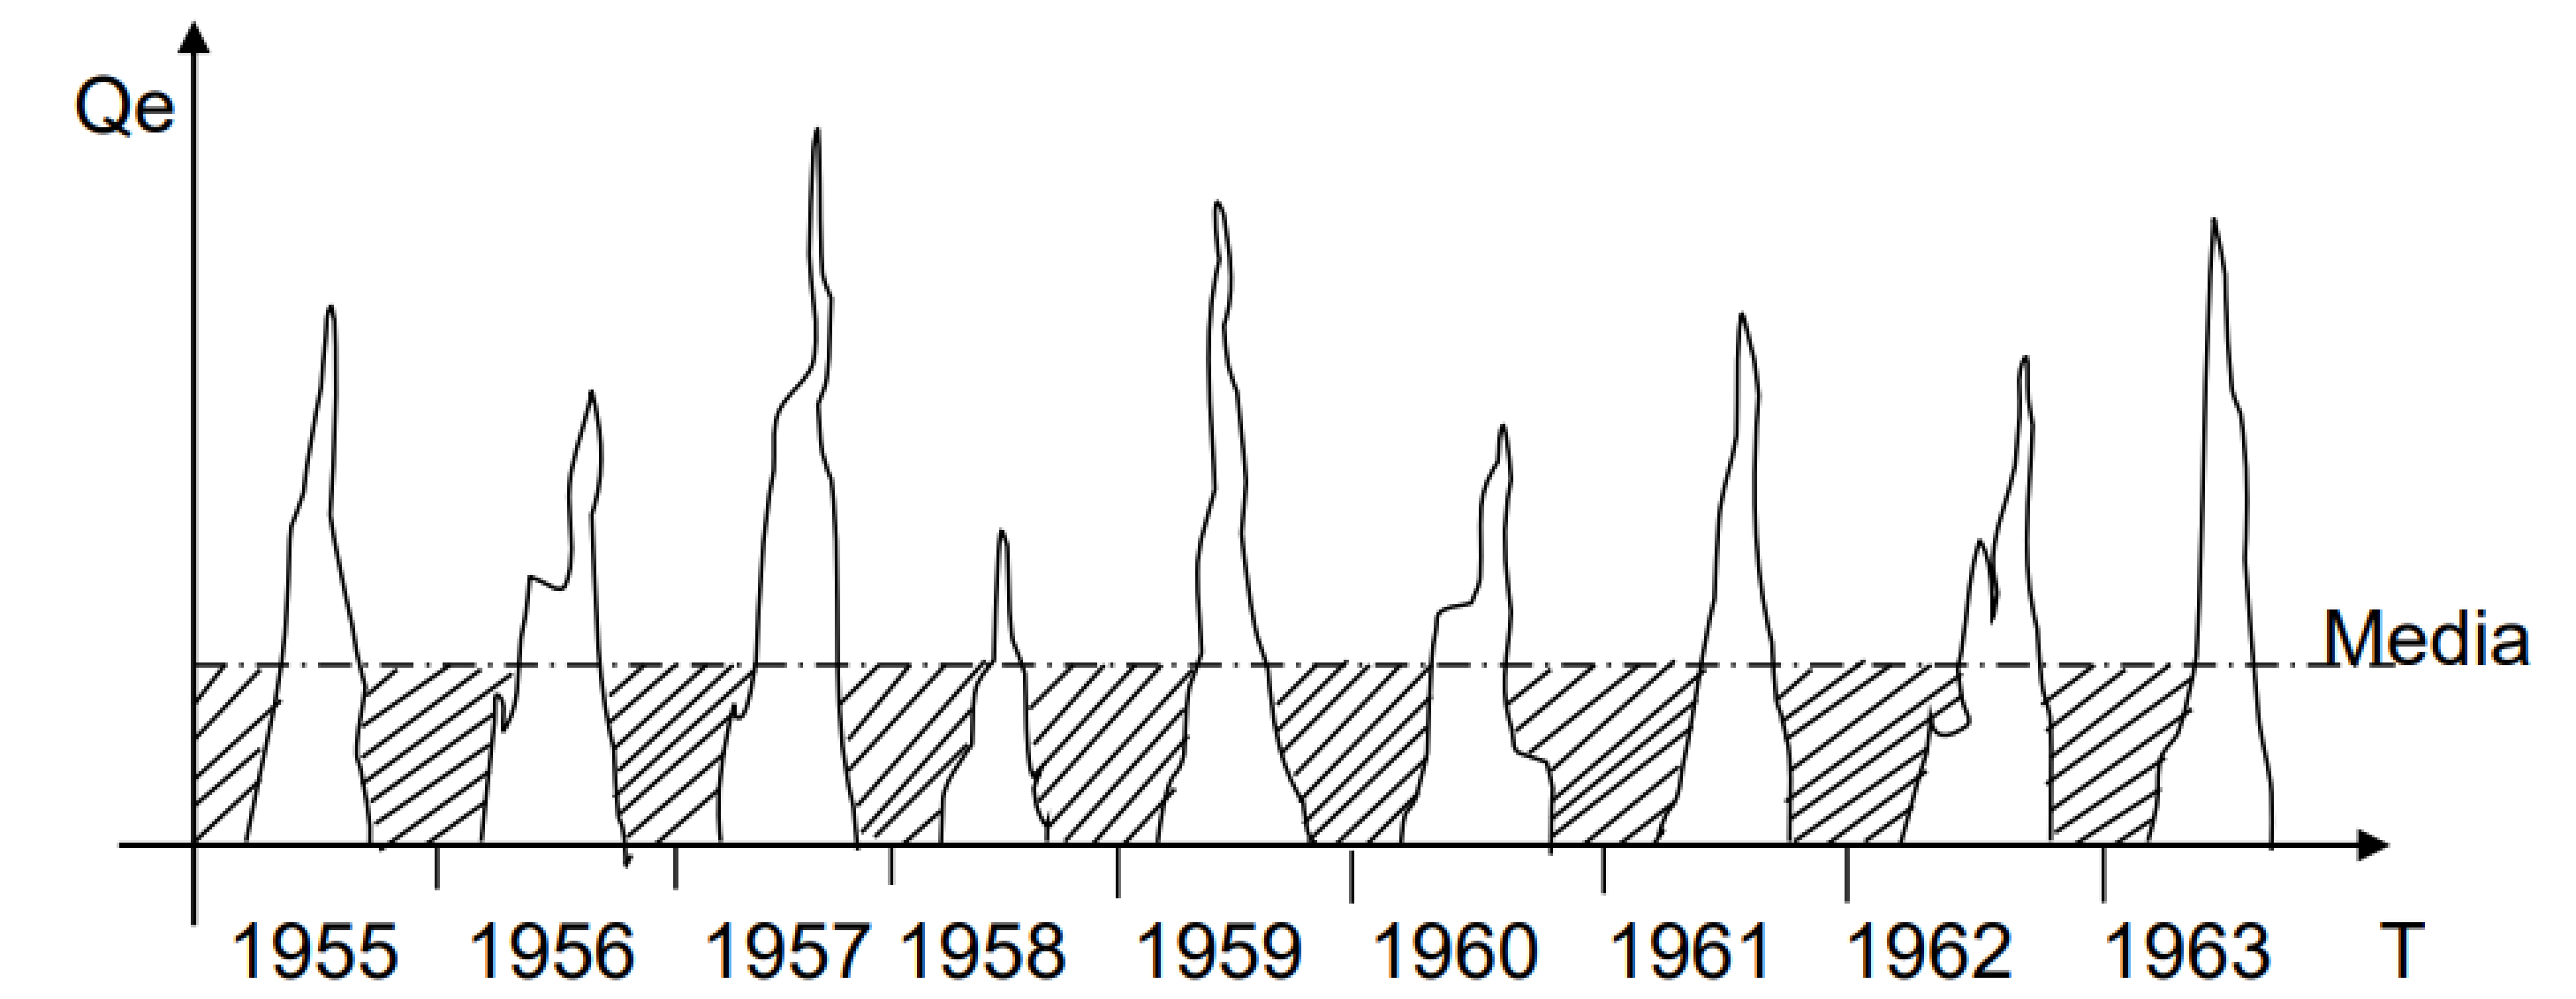
\includegraphics[width=0.5\textwidth]{fii20.png}}
	\caption{Hidrograma de una corriente intermitente.}
	\label{fii20}
\end{figure}
La necesidad de regularizar los escurrimientos de este tipo de corrientes, exige
la construcción de una \textbf{presa de almacenamiento}.
\begin{figure}[h!]
	\centerline{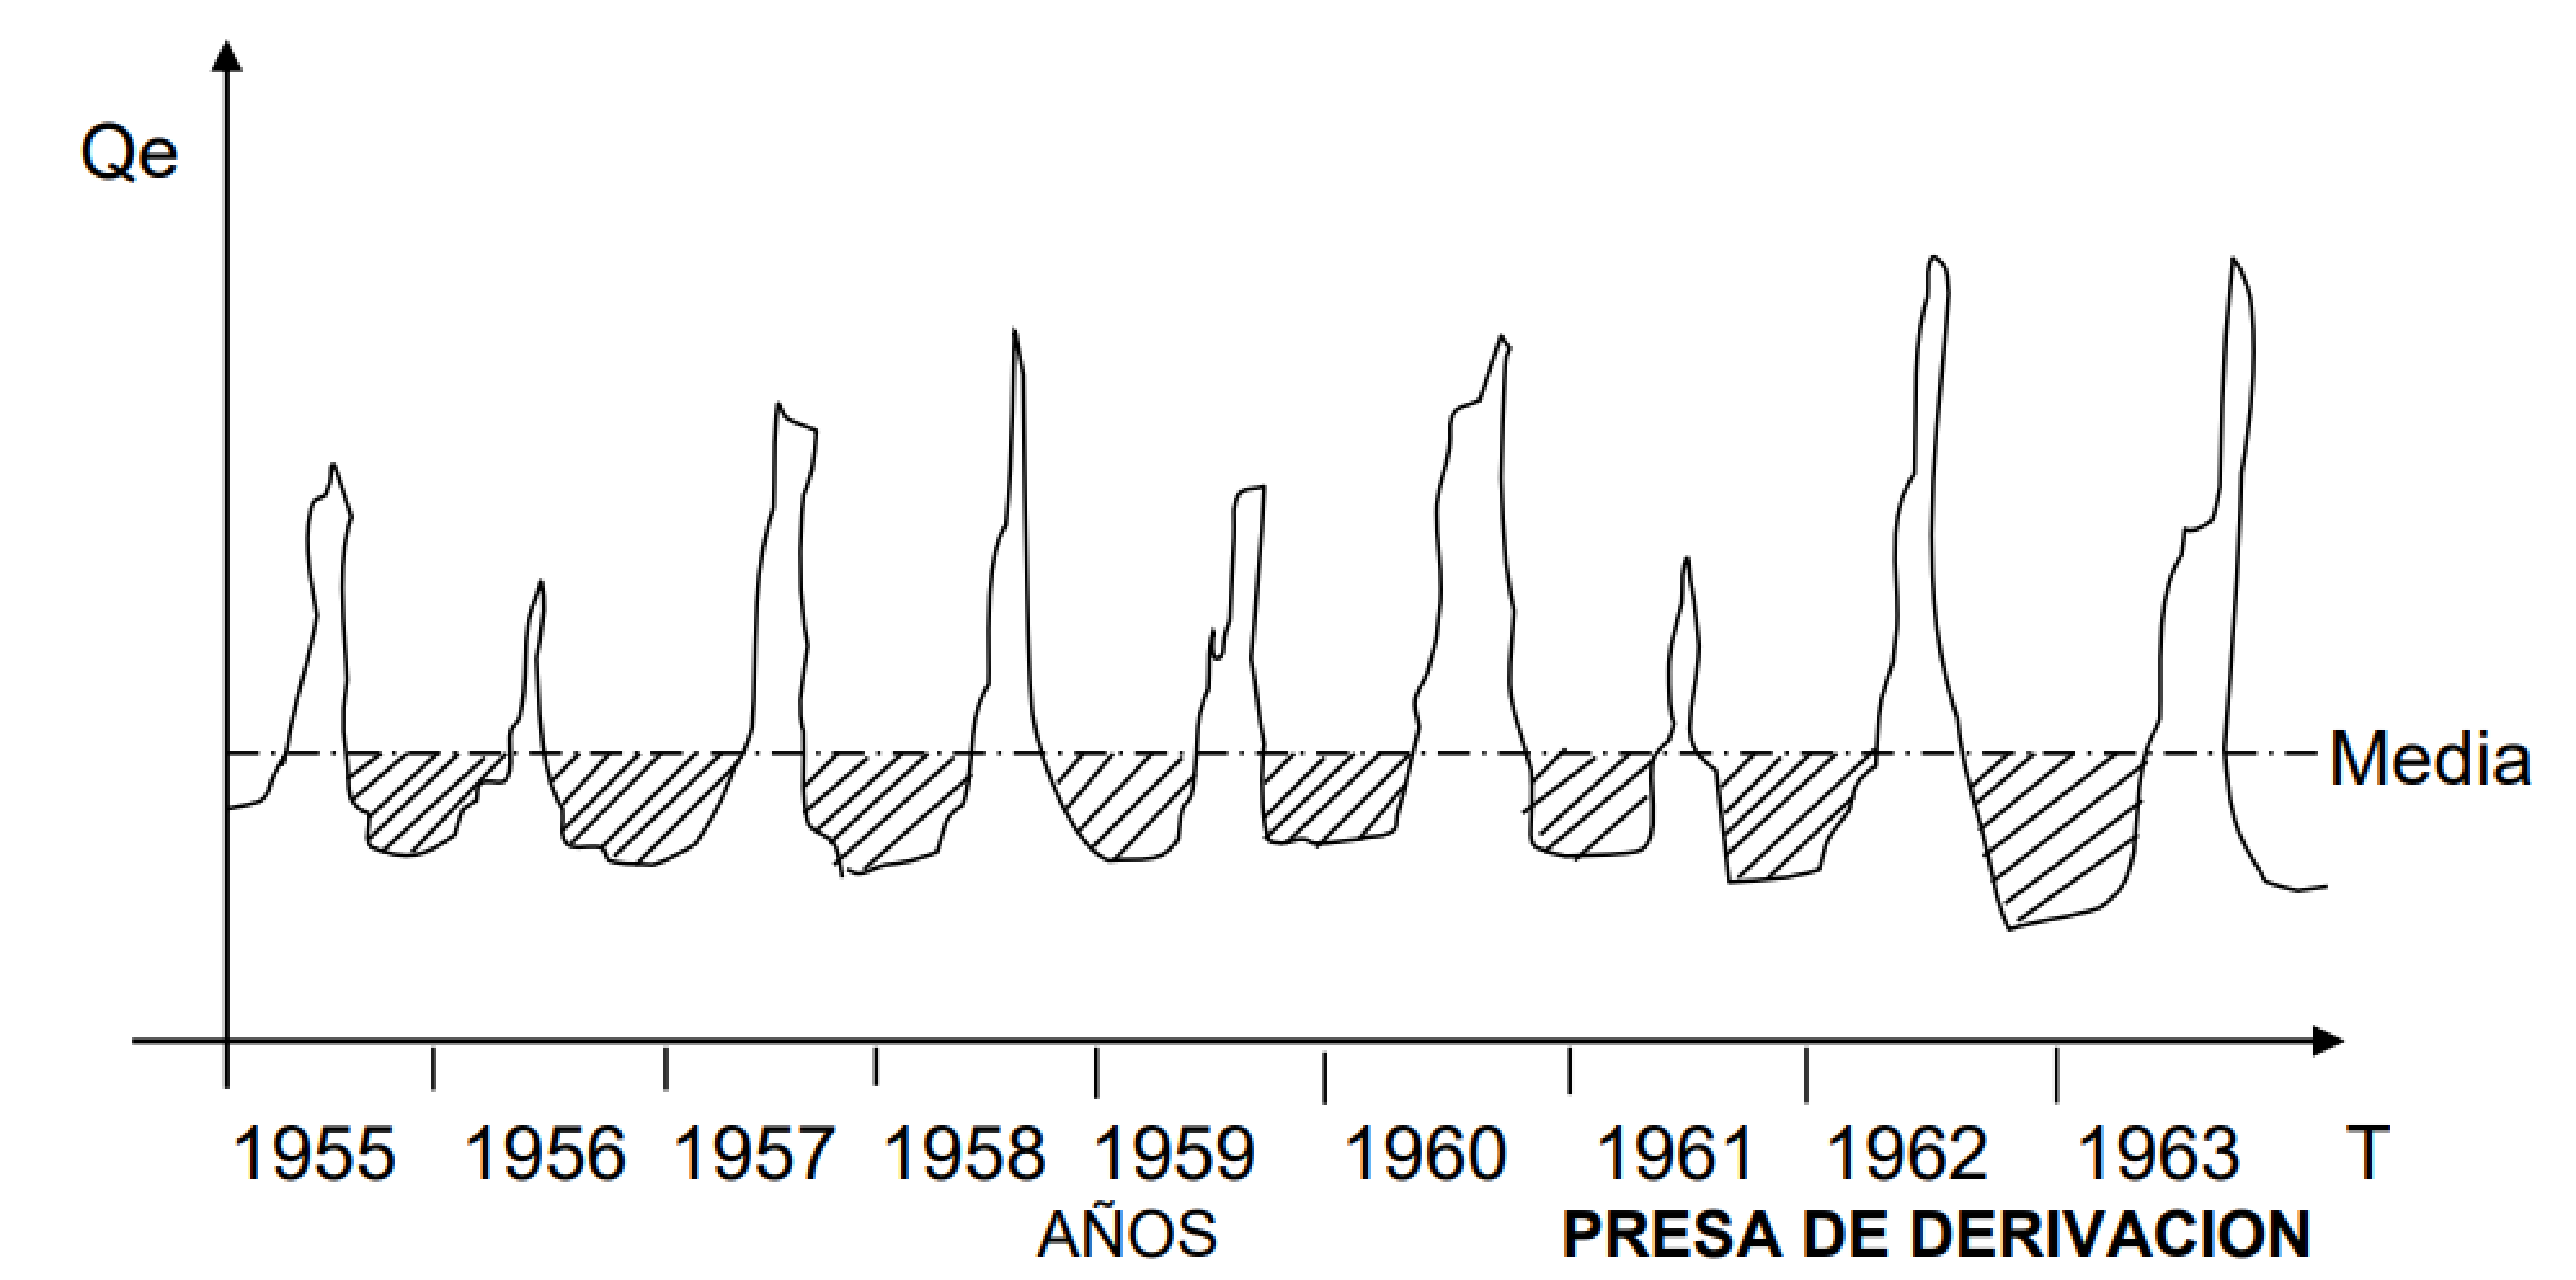
\includegraphics[width=0.5\textwidth]{fii21.png}}
	\caption{Hidrograma de una corriente permanente con caudales reducidos.}
	\label{fii21}
\end{figure}

\begin{figure}[h!]
	\centerline{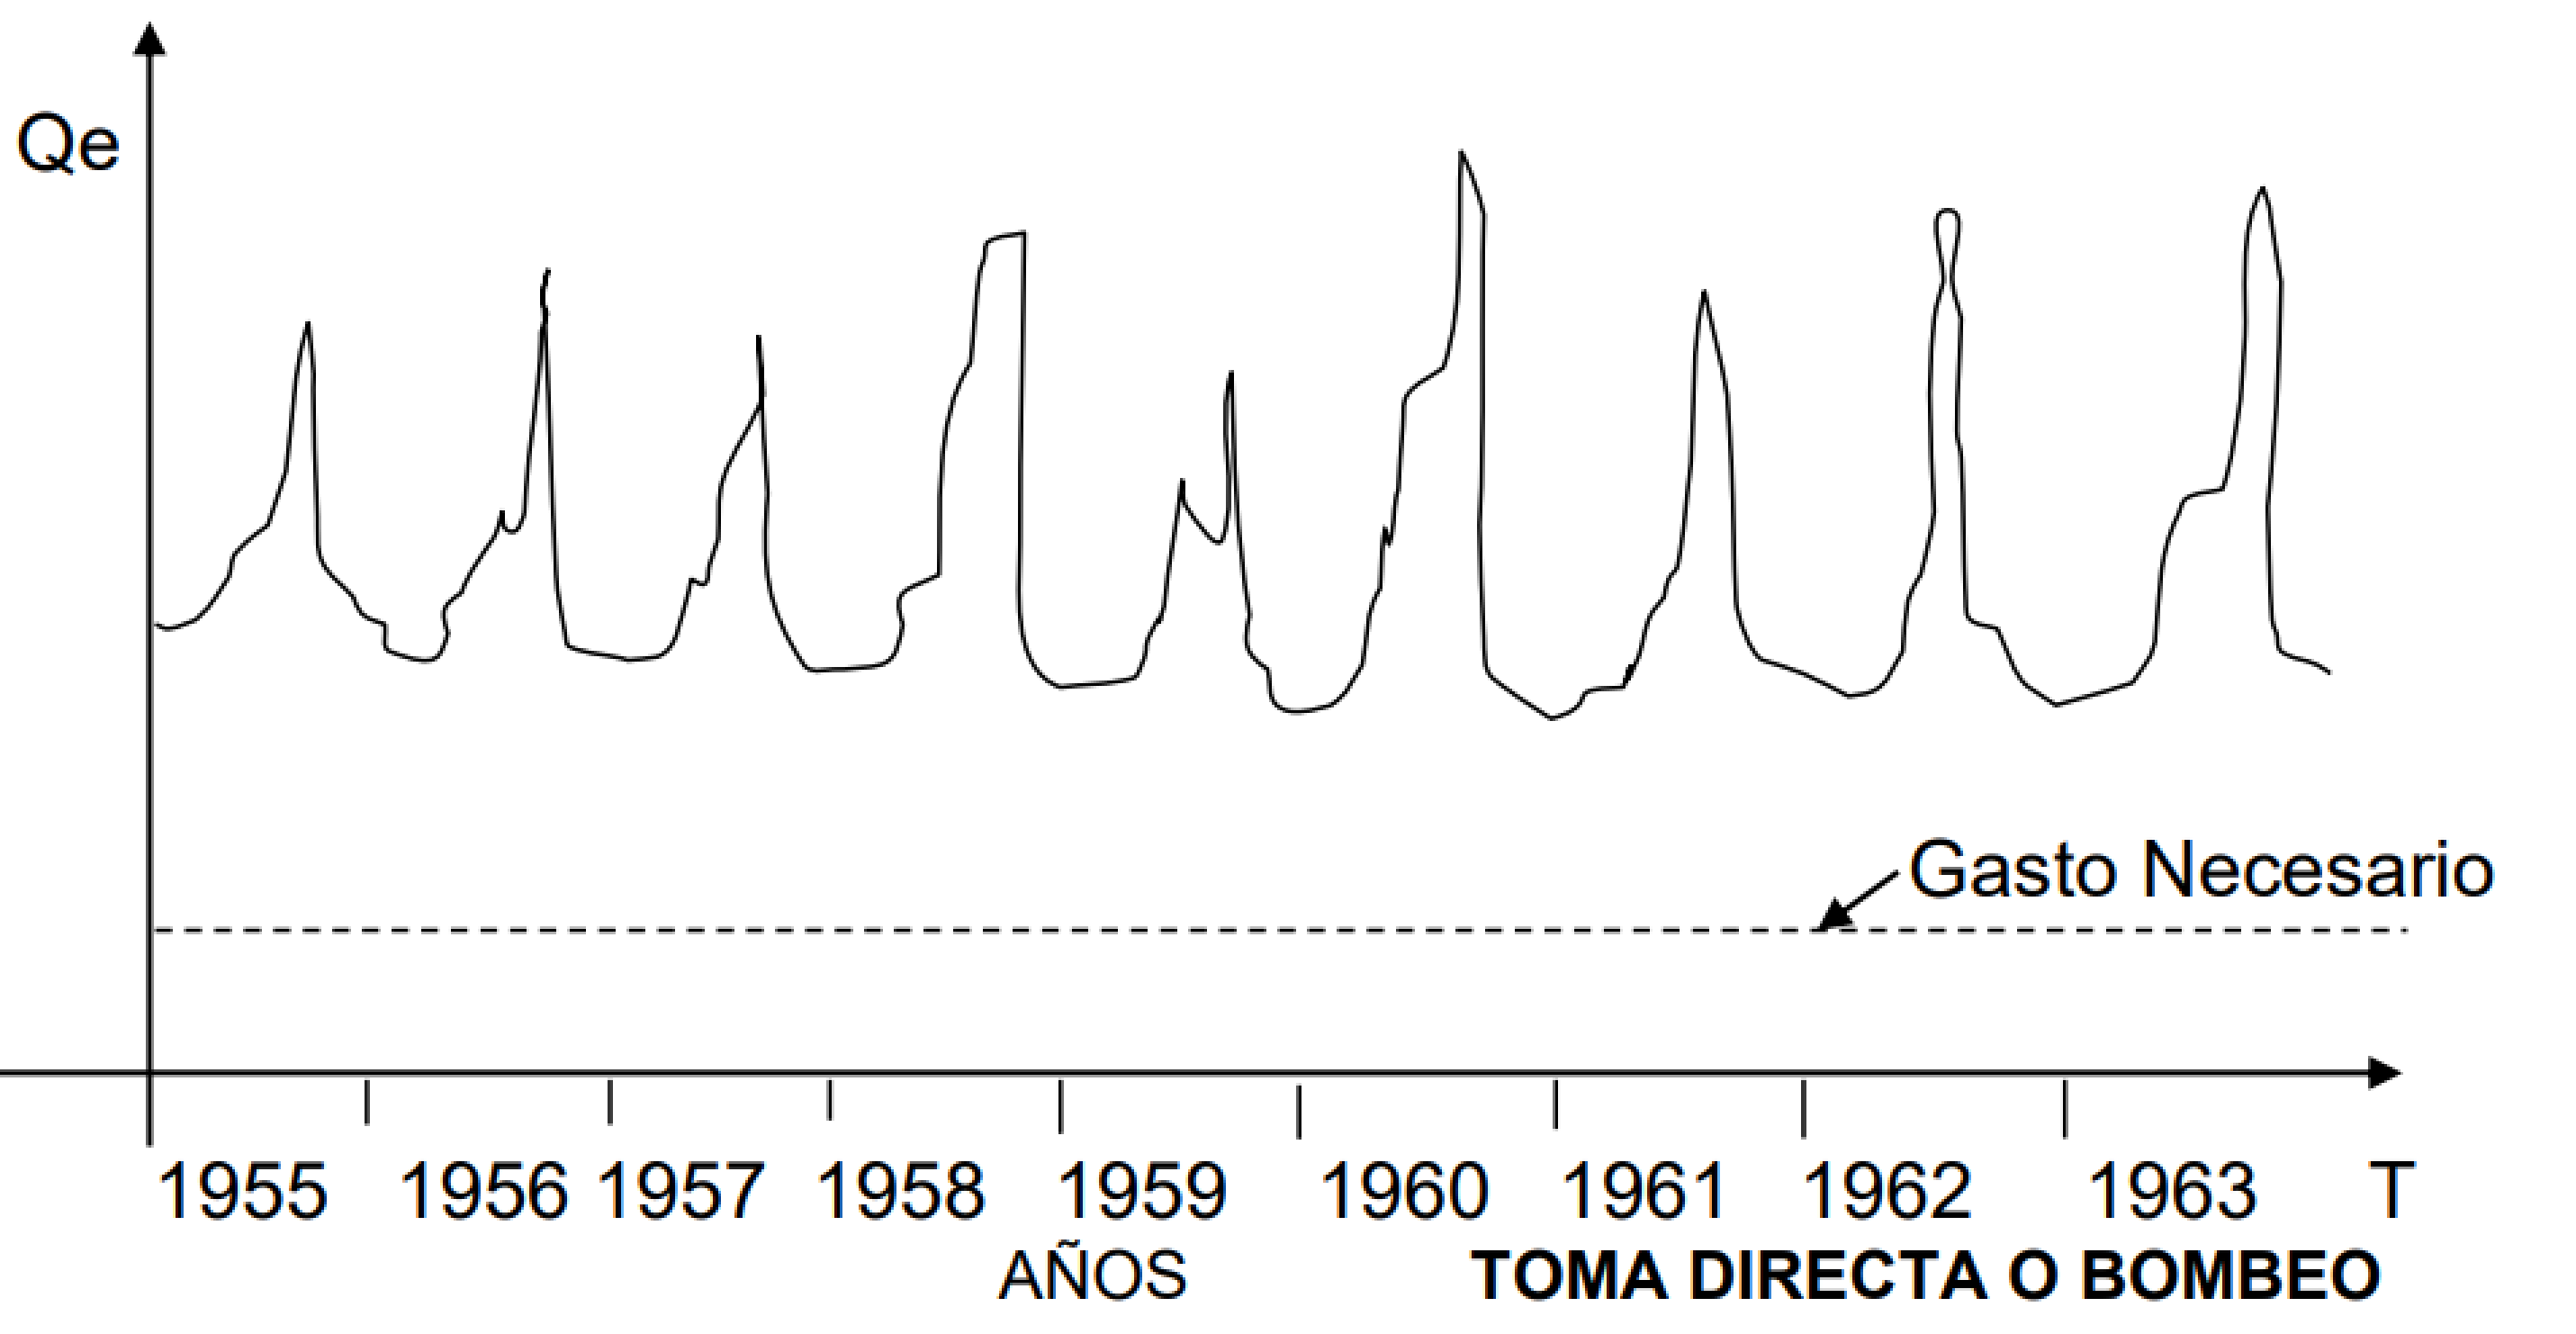
\includegraphics[width=0.5\textwidth]{fii22.png}}
	\caption{ Hidrograma de una corriente permanente con caudales acentuados.}
	\label{fii22}
\end{figure}

Las características de la corriente indica en principio el tipo de obra a construir. El estudio Hidrológico, comprende:

\begin{enumerate}
	\item Régimen del escurrimiento
	\item Régimen de demandas
	      \begin{enumerate}
		      \item Programa de cultivos
		      \item Plan de riegos
	      \end{enumerate}
\end{enumerate}


\begin{equation}
	L_{B}= \frac{V_{A.R.}}{S_{C.R.}}
\end{equation}

$L_{B} = (1{.}06m , 1{.}17m)$ (Promedio: $1{.}00m \approx 10,000 m^3$/Ha/año)

Donde $L_{B}$ es la lámina de riego bruta, en $m$, $V_{A.R.}$ Es el volumen de agua de riego, en $m^3$ y
$S_{C.R.}$ Superficie cosechada de riego, en $m^2 $

\subsubsection{Tipos de sistema de de Riego por Gravedad}

\begin{enumerate}
	\item \textbf{Con almacenamiento:} Este sistema de riego está conformado con una presa de almacenamiento como
	      fuente de abastecimiento principal, así como con una serie de canales y sus
	      estructuras que permiten llevar el agua de la presa hasta los lotes o parcelas de riego
	      donde se encuentran los cultivos.
	\item \textbf{Con almacenamiento y derivación}: Este sistema se presenta cuando la distancia entre la presa de almacenamiento
	      y la zona de riego es considerable, y entonces se utiliza un tramo de cauce como parte
	      del sistema de conducción, teniendo que proyectar una Presa derivadora aguas abajo
	      para poder extraer del mismo el agua y entregarla a un canal.
	\item \textbf{Mediante derivación:} Cuando por las condiciones del escurrimiento este se presenta en forma
	      permanente, presentándose en la época de estiaje un caudal de una magnitud
	      relativamente pequeña, entonces se puede plantear un sistema de riego por gravedad
	      mediante una derivación.
	\item \textbf{Con almacenamiento, derivación y bombeo:} Otras alternativas de explotación de las aguas superficiales, es cuando la zona
	      por beneficiar se encuentra en niveles superiores a donde se ubica la fuente de
	      abastecimiento, y entonces los aprovechamientos son por bombeo, si a esto se
	      adiciona que el origen del agua es de escurrimiento superficial en corriente intermitente
	      y la zona de riego se presenta a una cierta distancia de la fuente de abastecimiento,
	      entonces se presenta el Sistema de riego por gravedad con almacenamiento,
	      derivación y bombeo.
	\item \textbf{Mediante bombeo:} Cuando se tiene una fuente de abastecimiento cuyo origen del agua es
	      superficial, como un lago, laguna, o río, o su origen es subterráneo como manantiales
	      o galerías filtrantes, y el aprovechamiento se encuentra a niveles superiores a donde se
	      ubica la fuente entonces el sistema de riego por gravedad planteado es exclusivamente
	      por bombeo teniendo que conformarse una obra que se denomina Planta de Bombeo.
\end{enumerate}

\subsubsection{Partes constitutivas de un sistema de riego por gravedad}

El sistema de riego por gravedad a su vez se constituye por una serie de
subsistemas:

\begin{enumerate}
	\item Subsistema de almacenamiento
	\item Subsistema de conducción
	\item Subsistema de derivación
	\item Subsistema de distribución
	\item Subsistema de drenaje
	\item Subsistema de comunicaciones y obras diversas.
\end{enumerate}
\begin{figure}[h!]
	\centerline{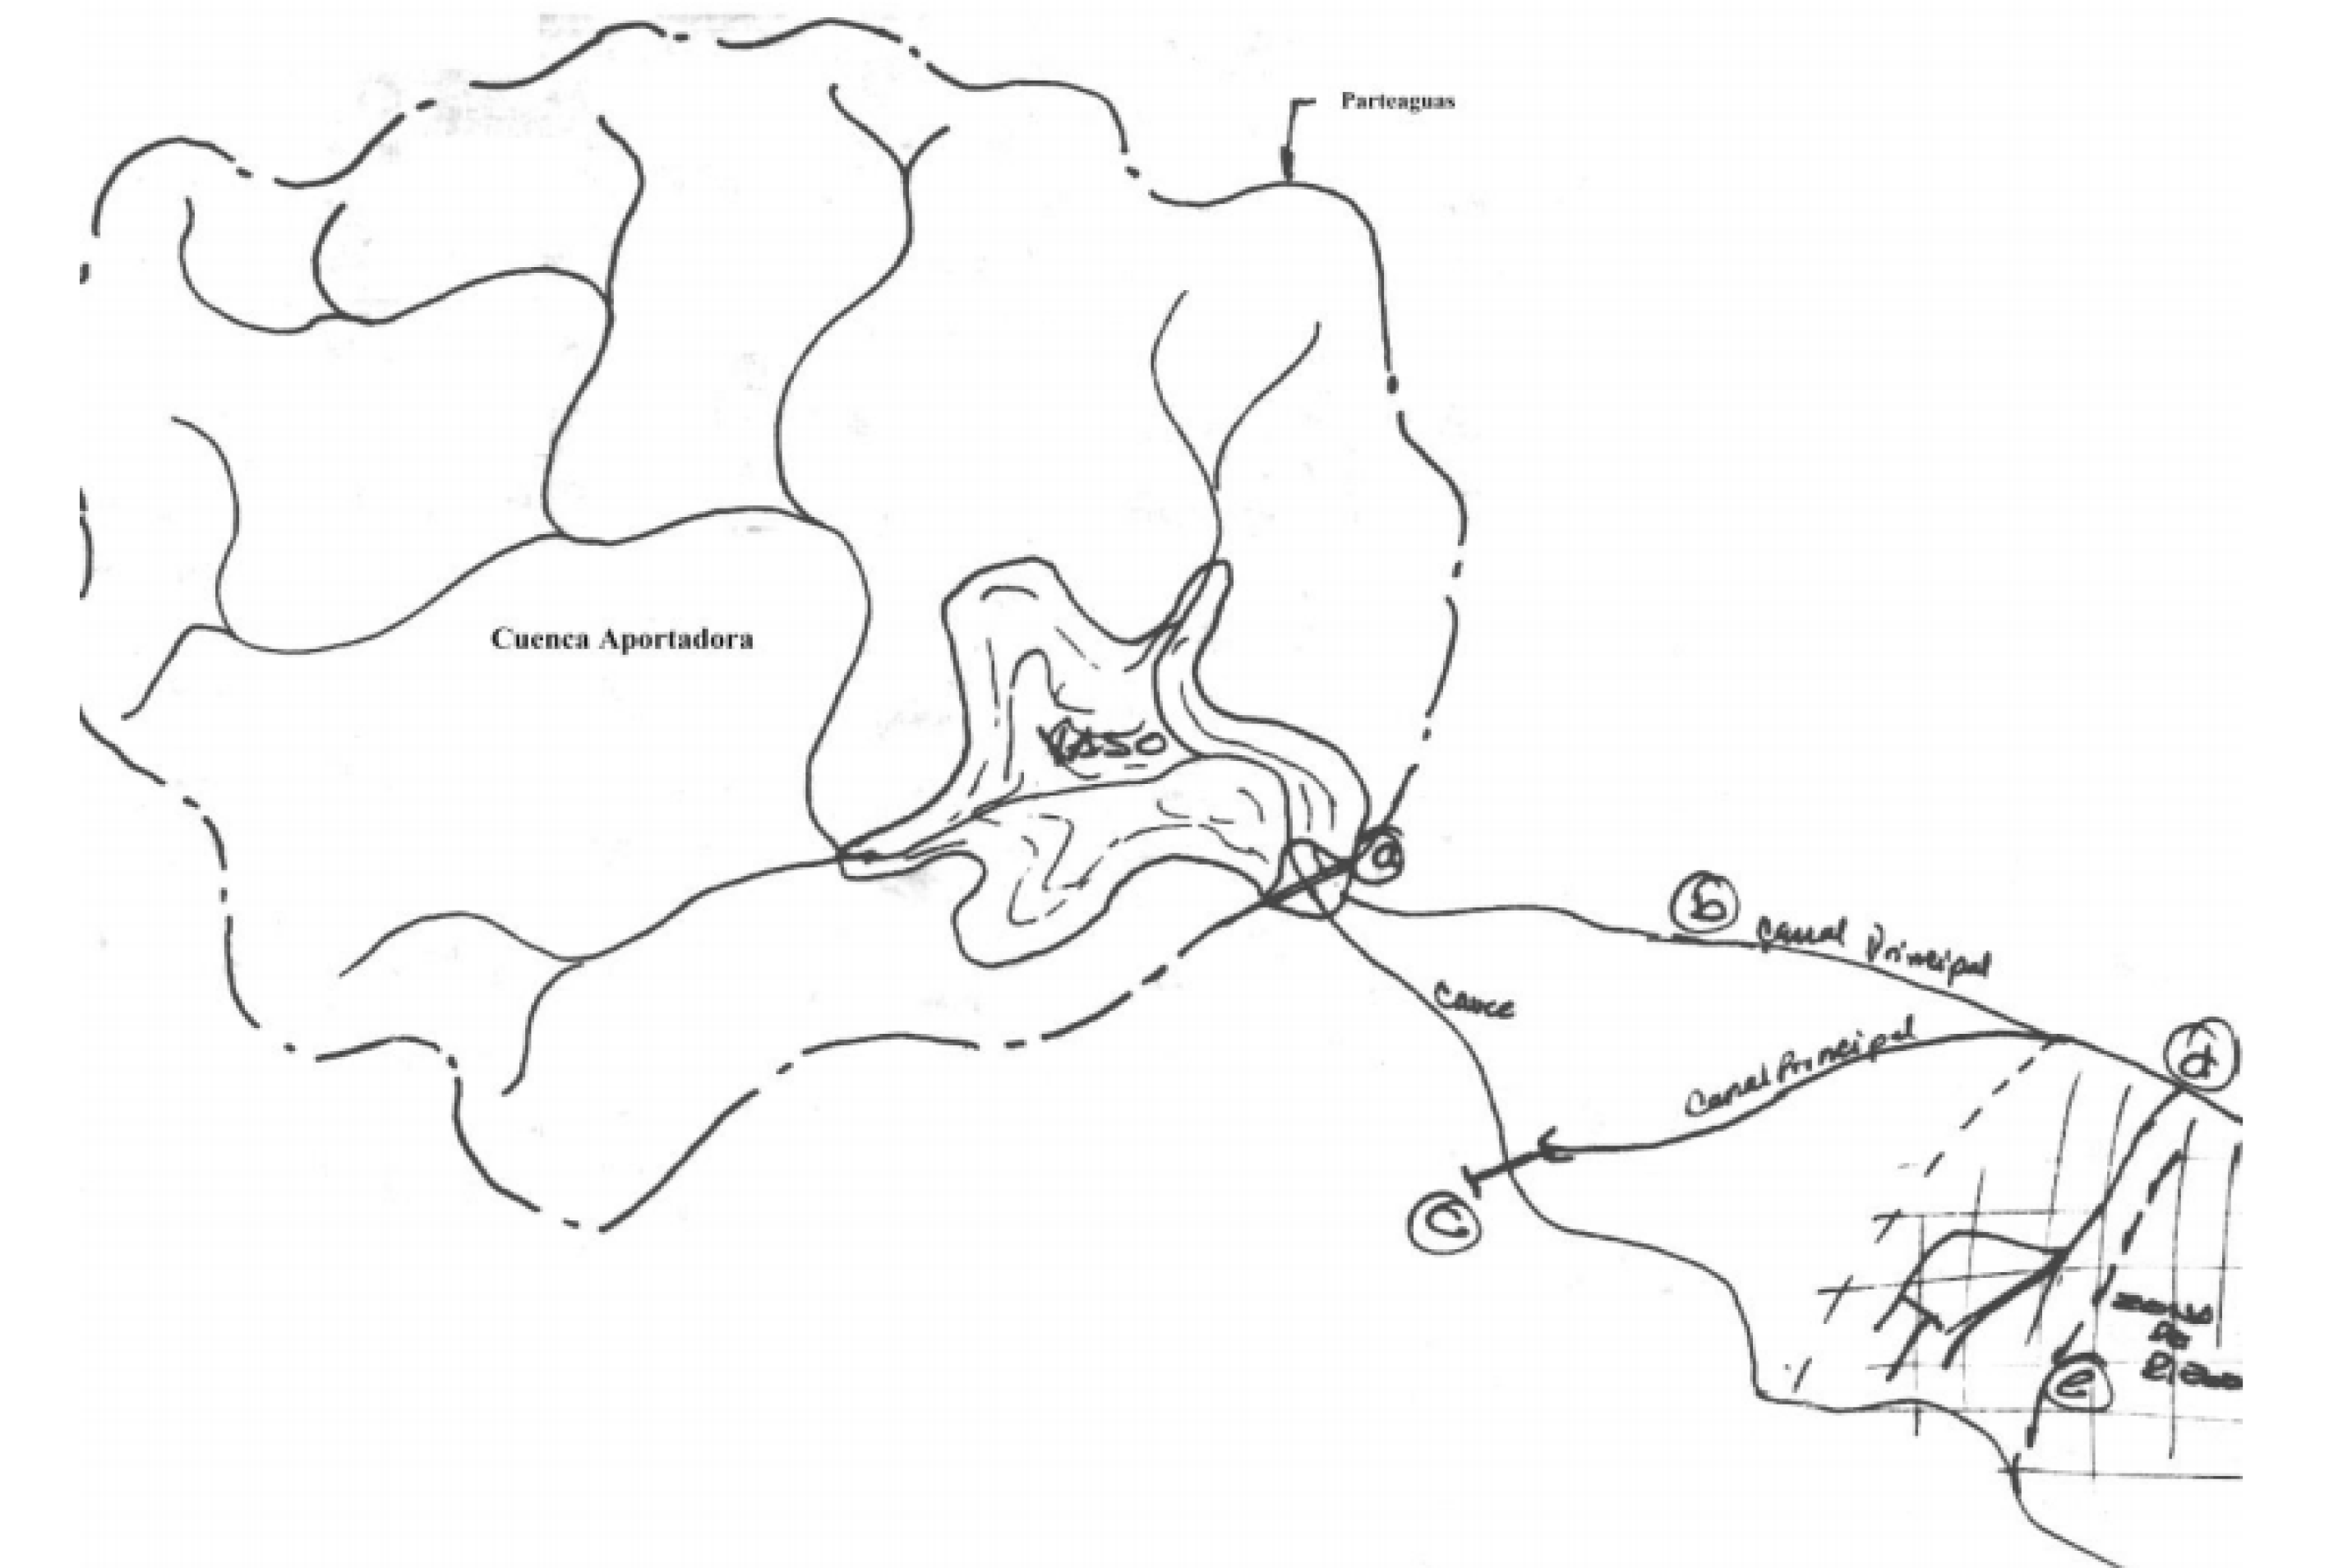
\includegraphics[width=0.7\textwidth]{fii23.png}}
	\caption{Esquema genérico de un sistema de riego por gravedad completo.}
	\label{fii23}
\end{figure}

\subsubsection{Partes constitutivas de un sistema de riego por bombeo.}

En general las partes constitutivas de un sistema de riego por bombeo son las
mismas que las de un sistema de riego por gravedad, con la única diferencia es que se
ubica a continuación de la fuente de abastecimiento una planta de bombeo que va a
permitir ubicar el agua a un nivel suficiente para dominar toda la superficie de riego
mediante gravedad, buscando que esta ubicación sea en la forma más económica a
través de ubicar una mínima diferencia de niveles y en el menor recorrido posible.

\begin{figure}[h!]
	\centerline{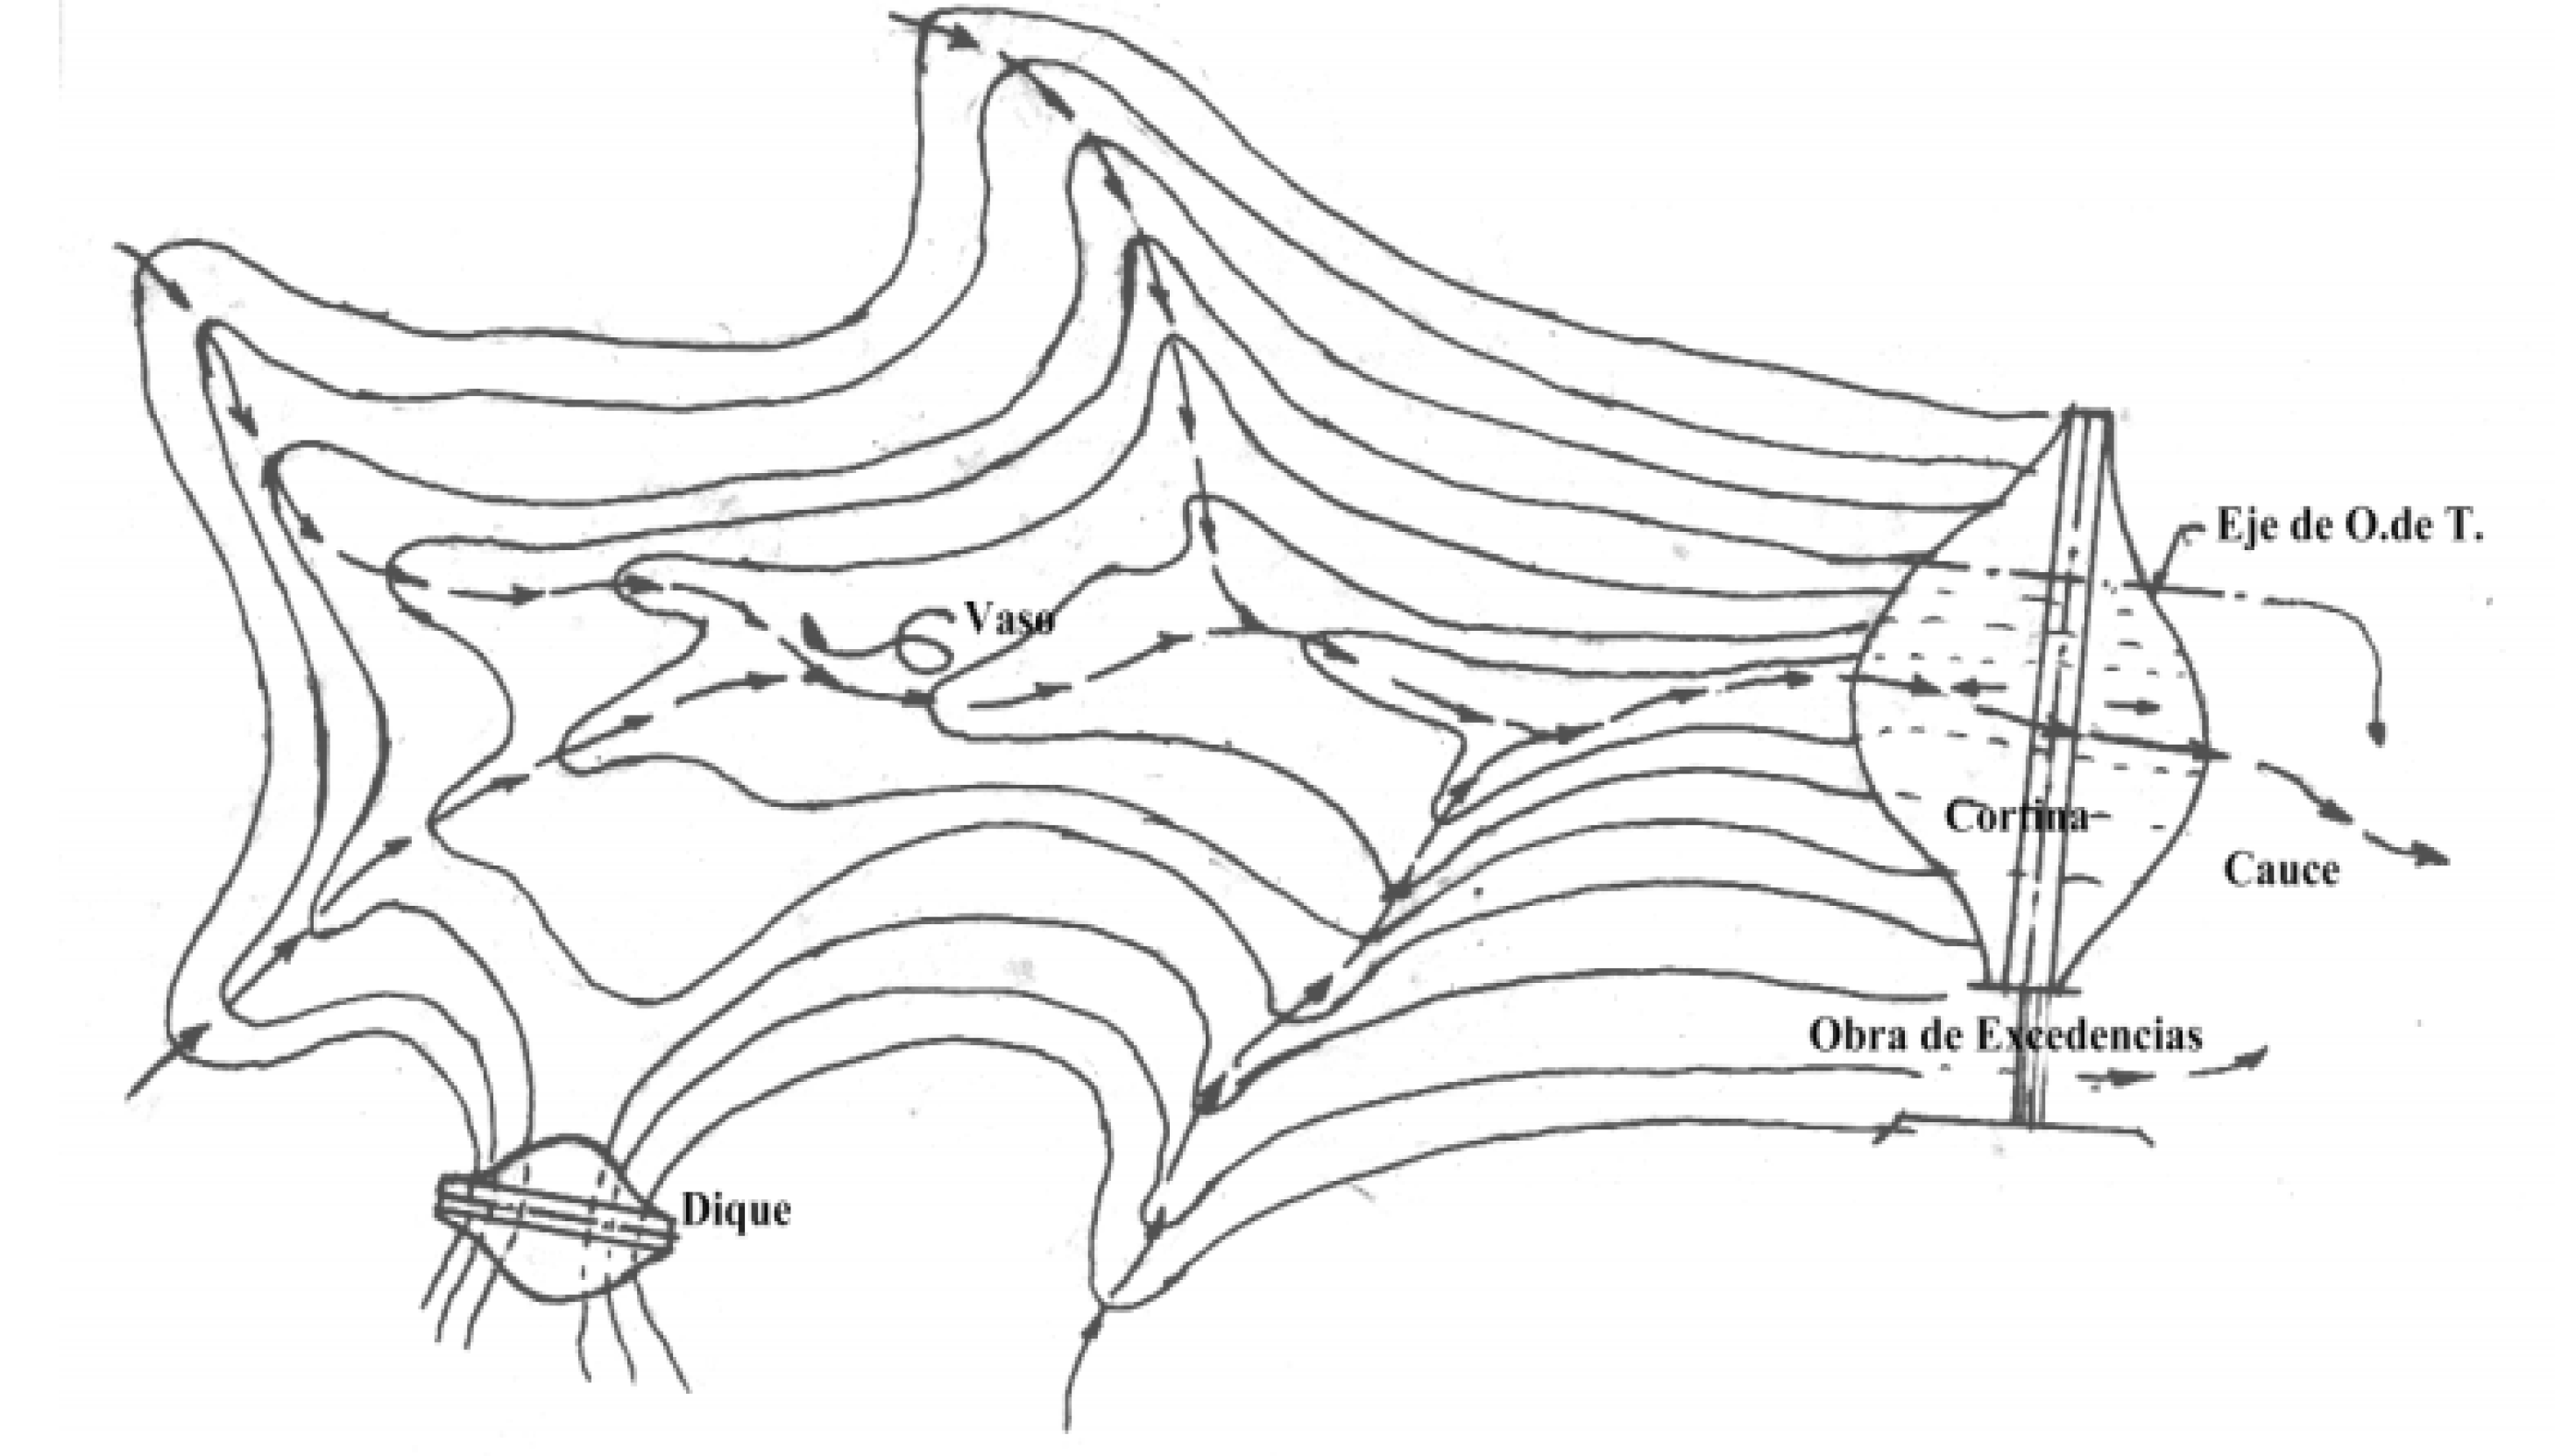
\includegraphics[width=0.5\textwidth]{fii24.png}}
	\caption{Planta Esquemática de Presa y Vaso de almacenamiento}
	\label{fii24}
\end{figure}

\section{Sistema de almacenamiento}
\subsection{Partes constitutivas y funciones}
\begin{definition}[Obra de retención (o cortina)]
	La función de esta es retener las aguas para
	formar el vaso de almacenamiento y regular los escurrimientos del cauce.
\end{definition}

\begin{definition}[Obra de toma]
	La función de esta obra es manejar las extracciones para
	satisfacer la demanda que los diferentes beneficios exigen.
\end{definition}

\begin{definition}[Obra de excedencias]
	La función es dar salida a las aguas de escurrimiento que
	no pueden ser almacenadas por haber llegado a un cierto nivel que muestra la
	capacidad total.
\end{definition}

Estas tres estructuras, por lo general forman las \textbf{presa de Almacenamiento}.

\begin{definition}[Diques de cierre]
	La función es ayudar a la cortina al cierre del vaso, en puertos
	naturales independientes de la boquilla.
\end{definition}

\subsection{Elementos naturales y sus condiciones de los sistemas de almacenamiento}

\begin{definition}[Cuenca]
	Es la superficie de terreno limitada por la línea del parteaguas, en la cual el agua
	de lluvia precipitada dentro del área, escurre para ser drenada por el río o arroyo,
	desde su nacimiento hasta el sitio de la boquilla.
	Las características de tamaño, forma, vegetación, pendientes, corrientes, etc$\dots$
	son condiciones que influyen en el escurrimiento y adecuada alimentación al vaso.
\end{definition}

\begin{definition}[Vaso de almacenamiento]
	Valle en cual se puede crear un receptáculo topográfico para almacenar agua,
	mediante el cierre de una boquilla con una estructura para formar un lago artificial.
	Las características de capacidad e impermeabilidad, son condiciones favorables
	para un adecuado almacenamiento. Topografía: implica Gráfica de Áreas-Capacidades;
	Geología: implica Impermeabilidad; Problemas: Calizas cavernosas (yeso y grietas).
\end{definition}

\begin{definition}[Boquilla]
	Estrechamiento topográfico de un valle donde se construye la estructura de
	retención o cortina. Condiciones favorables: Resistencia, impermeabilidad, topografía implica
	Topografía Forma y tamaño; Geología implica Resistencia e impermeabilidad
\end{definition}

\begin{definition}[Cauce]
	Conducto natural por el cual escurre el agua. Su estudio es importante por el
	acarreo de sedimentos, así como por la permeabilidad.
\end{definition}

\subsection{Gráfica Áreas Capacidades}

Un vaso de almacenamiento topográficamente es un valle natural que tiene
como base un cauce por el cual escurre el agua que se ha precipitado en el área de la
cuenca y la cual es cerrada en el sitio denominado boquilla y sobre la que se proyecta y
construye una cortina o presa, cerrando así el sitio y conformando un gran lago
artificial.

Para conocer e identificar la forma de un vaso de almacenamiento es necesario
efectuar previamente un levantamiento topográfico que permita determinar su
capacidad a diferentes alturas de la cortina, para conocer las áreas de embalse a
diferentes elevaciones, con el objeto de poder estimar las pérdidas por evaporación, así
mismo el poder contar con un apoyo para la realización de los diferentes estudios
necesarios para poder cumplir con las exigencias que plantea el proyecto de una presa
de almacenamiento, entre otros los estudios geológicos que permitan conocer el grado
de impermeabilidad del vaso, así como el poder identificar la superficie de las
propiedades inundadas que sirvan de base para las indemnizaciones correspondientes
ante las afectaciones que necesariamente tendrán que presentarse.

\begin{figure}[h!]
	\centerline{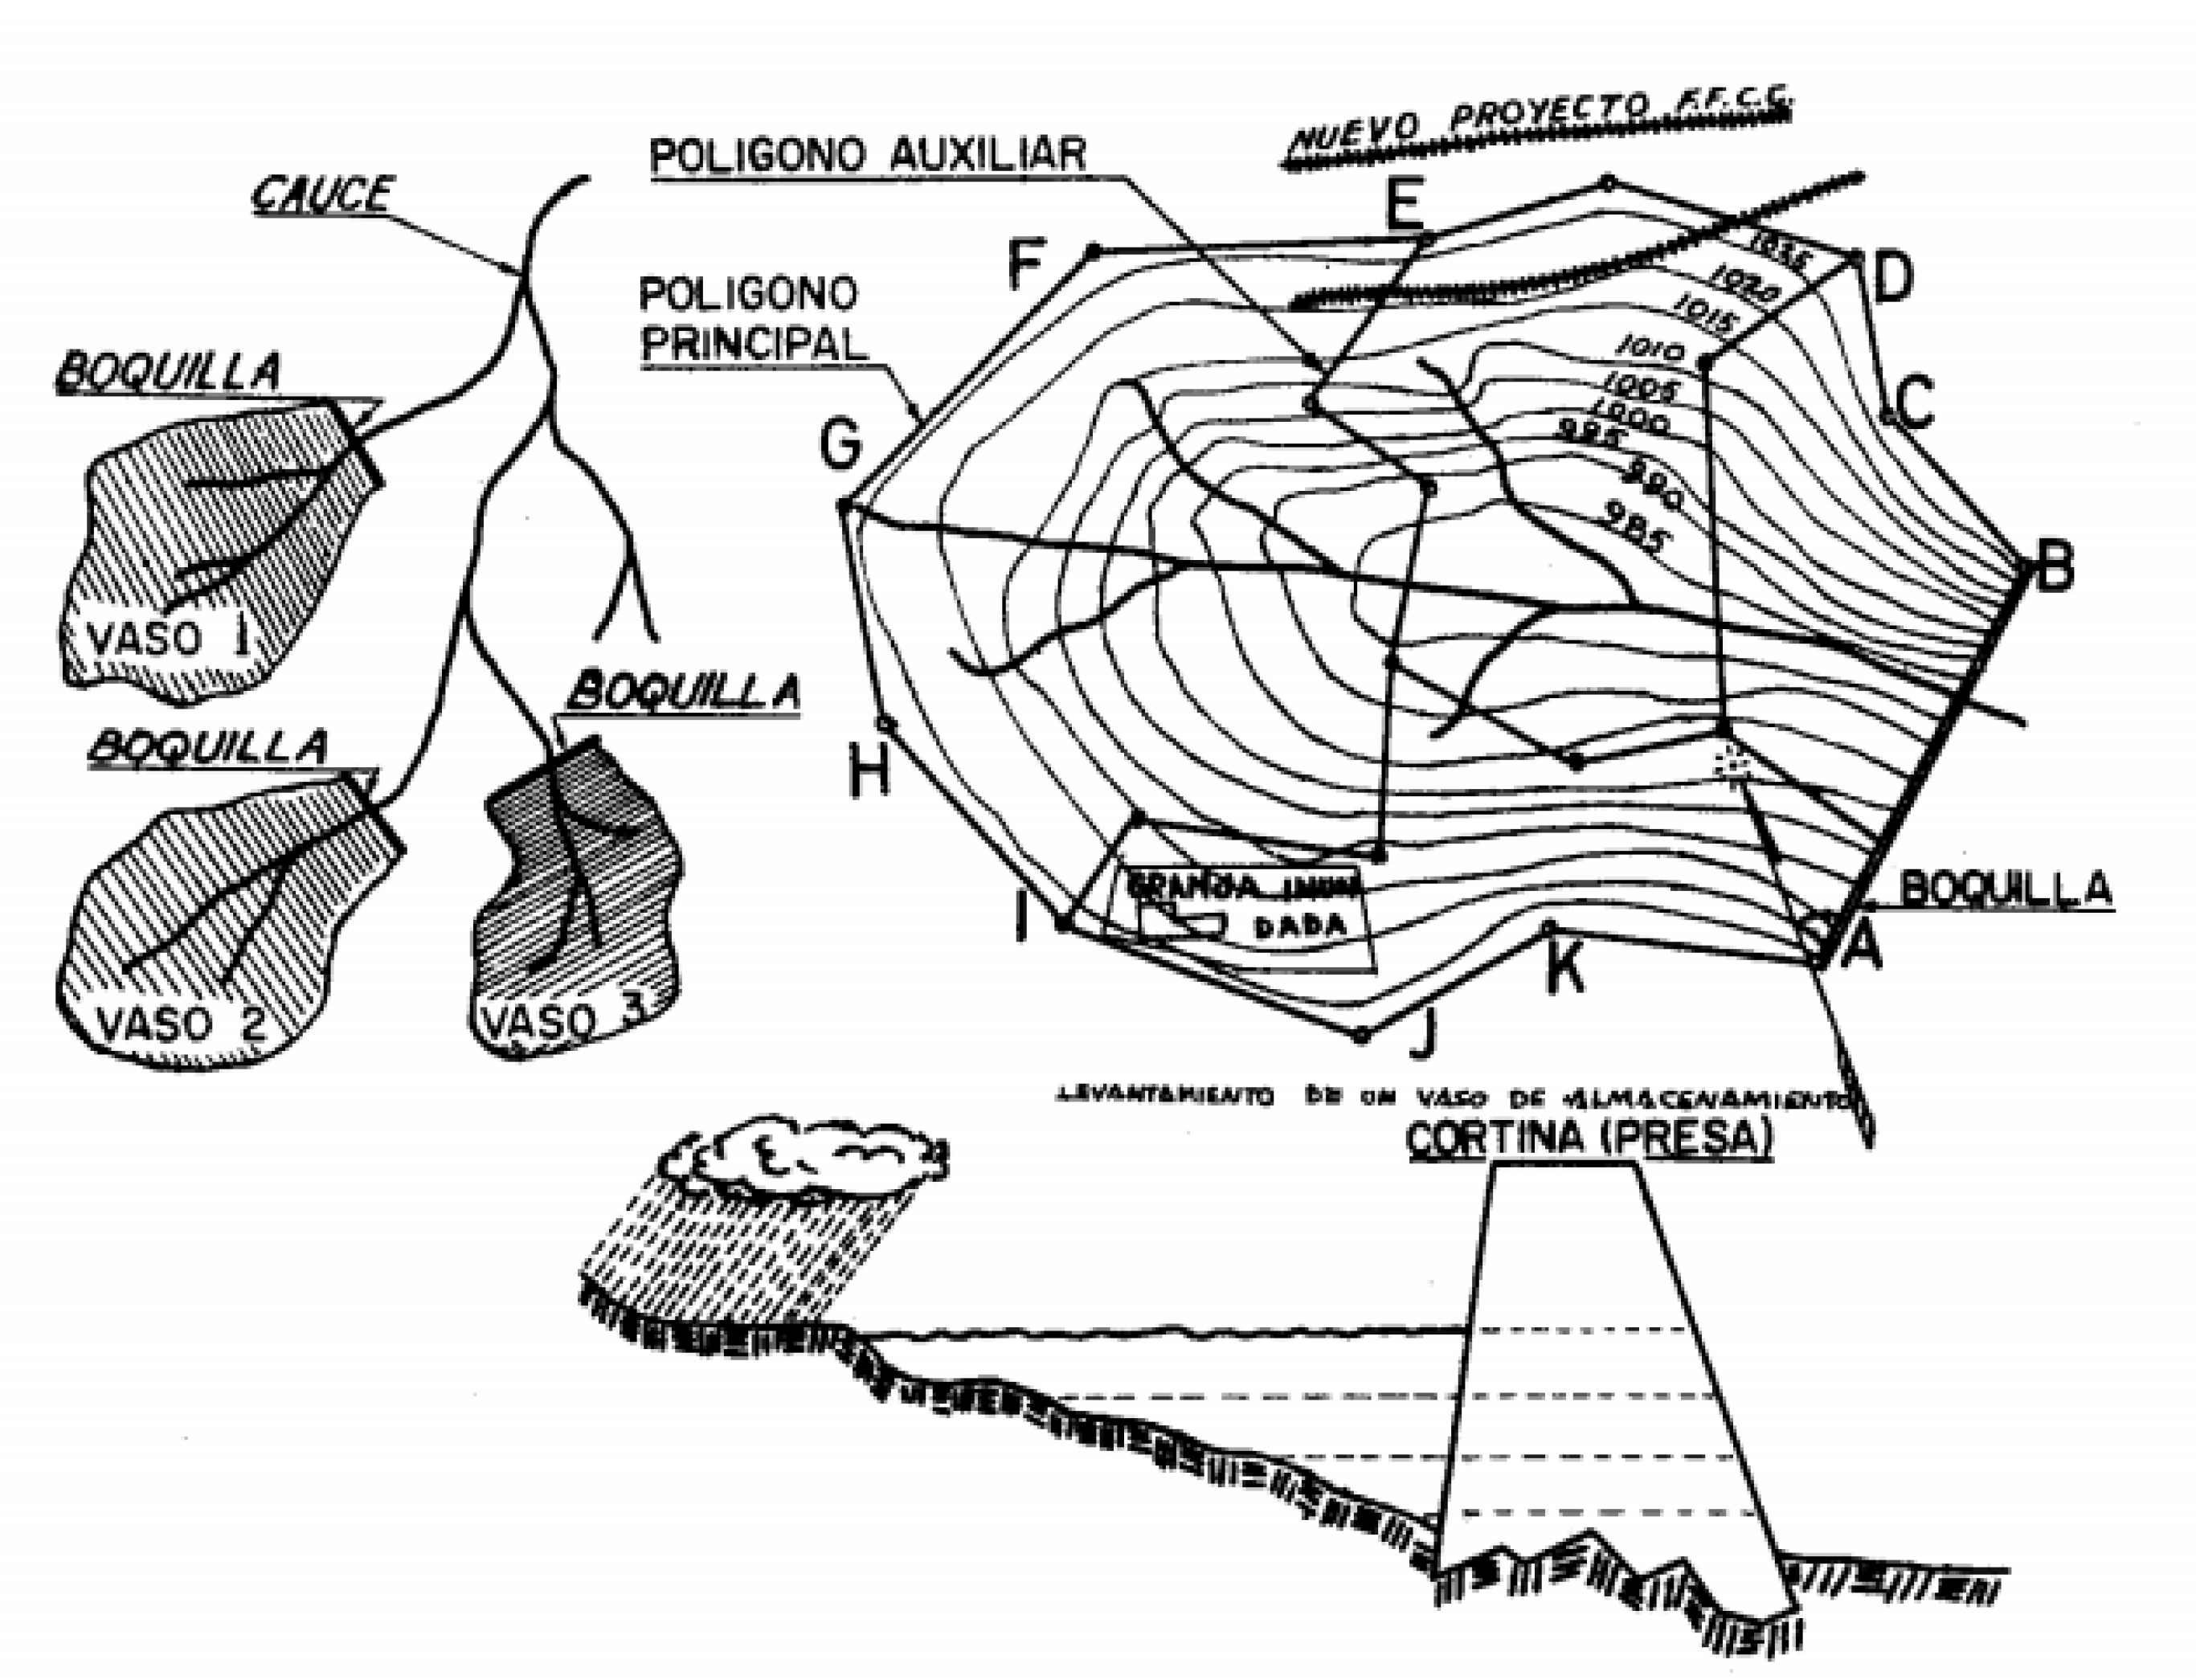
\includegraphics[width=0.5\textwidth]{fii25.png}}
	\caption{Levantamiento topográfico de un vaso de almacenamiento}
	\label{fii25}
\end{figure}

Para poder construir las gráficas de Áreas y Capacidades, se
delimitará el vaso de almacenamiento trazando la línea que corresponde al eje
probable de la cortina, que cerrará desde el fondo del cauce, hasta la curva
correspondiente al nivel probable de las aguas máximas.
El área de cada una de las curvas de nivel, limitada hasta el eje probable de la
cortina se obtiene por medio de un integrador mecánico (planímetro). Se hace la
determinación de las áreas, desde la correspondiente al fondo del cauce, hasta la
correspondiente al nivel probable de las aguas máximas.
El volumen entre dos curvas de nivel consecutivas se obtiene multiplicando la
semisuma de las dos áreas, por la diferencia de elevaciones entre las dos curvas. Así
si la equidistancia es de $1m$, y el volumen comprendido entre las curvas cuyas
elevaciones son la $152m$ y la $153m$, el volumen está dado por:
\begin{equation}
	V_{152-153}= \left(\frac{S_{152}+S_{153}}{2} \right) \times 1{.}0
\end{equation}
La suma de elevaciones parciales, da la capacidad del vaso hasta la elevación
requerida. Con estos datos se forma una tabla y posteriormente se construye la
Gráfica.
\begin{figure}[h!]
	\centerline{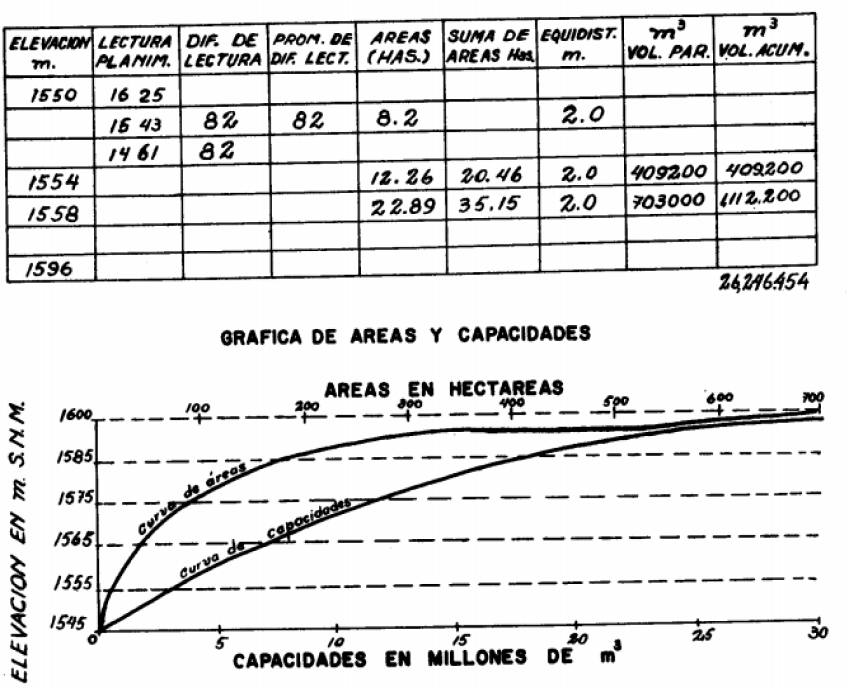
\includegraphics[width=0.5\textwidth]{fii26.png}}
	\caption{Gráfica de Áreas y capacidades en un vaso de almacenamiento.}
	\label{fii26}
\end{figure}
La graficación anterior es conveniente efectuarse en papel milimétrico bajo una
escala adecuada que permita hacer una lectura precisa y confiable en las elevaciones,
áreas y capacidades.

\subsection{Capacidades de almacenamiento y altura de la presa}
\begin{enumerate}
	\item \textbf{Capacidades de almacenamiento y Elevaciones físicas:} Las capacidades fundamentales que identifican a un almacenamiento son:
	      \begin{enumerate}
		      \item \textbf{Capacidad muerta $(C_{M})$:} es el volumen del almacenamiento el cual por su
		            condición nunca puede ser extraído del vaso por gravedad, para satisfacer beneficios
		            que se encuentren aguas abajo del mismo, y queda conformado con el volumen de
		            azolves y otros (Volumen para cría de peces, volumen para recreación y turismo,
		            volumen para abrevadero de ganado, etc$\dots$). Esta capacidad queda definida por el Nivel
		            de Almacenamiento mínimo \textbf{(N.A.min.)} la cual a su vez identifica a la cota física de la
		            obra de toma.
		      \item \textbf{Capacidad Total del almacenamiento \textbf{(CTA)}} es el volumen máximo que
		            puede ser retenido dentro del vaso, para cuando se tienen vertedores de cresta libre.
		            Esta capacidad queda definida por el Nivel de Aguas Normales (N.A.N.), algunos
		            autores le denominan N.A.M.O. (Nivel de Aguas Máximas de Operación), esta cota
		            identifica la cota física correspondiente al nivel de la cresta del vertedor de excedencias
		            (Obra de excedencias) cuando este tiene descarga libre.
		            \begin{figure}[h!]
			            \centerline{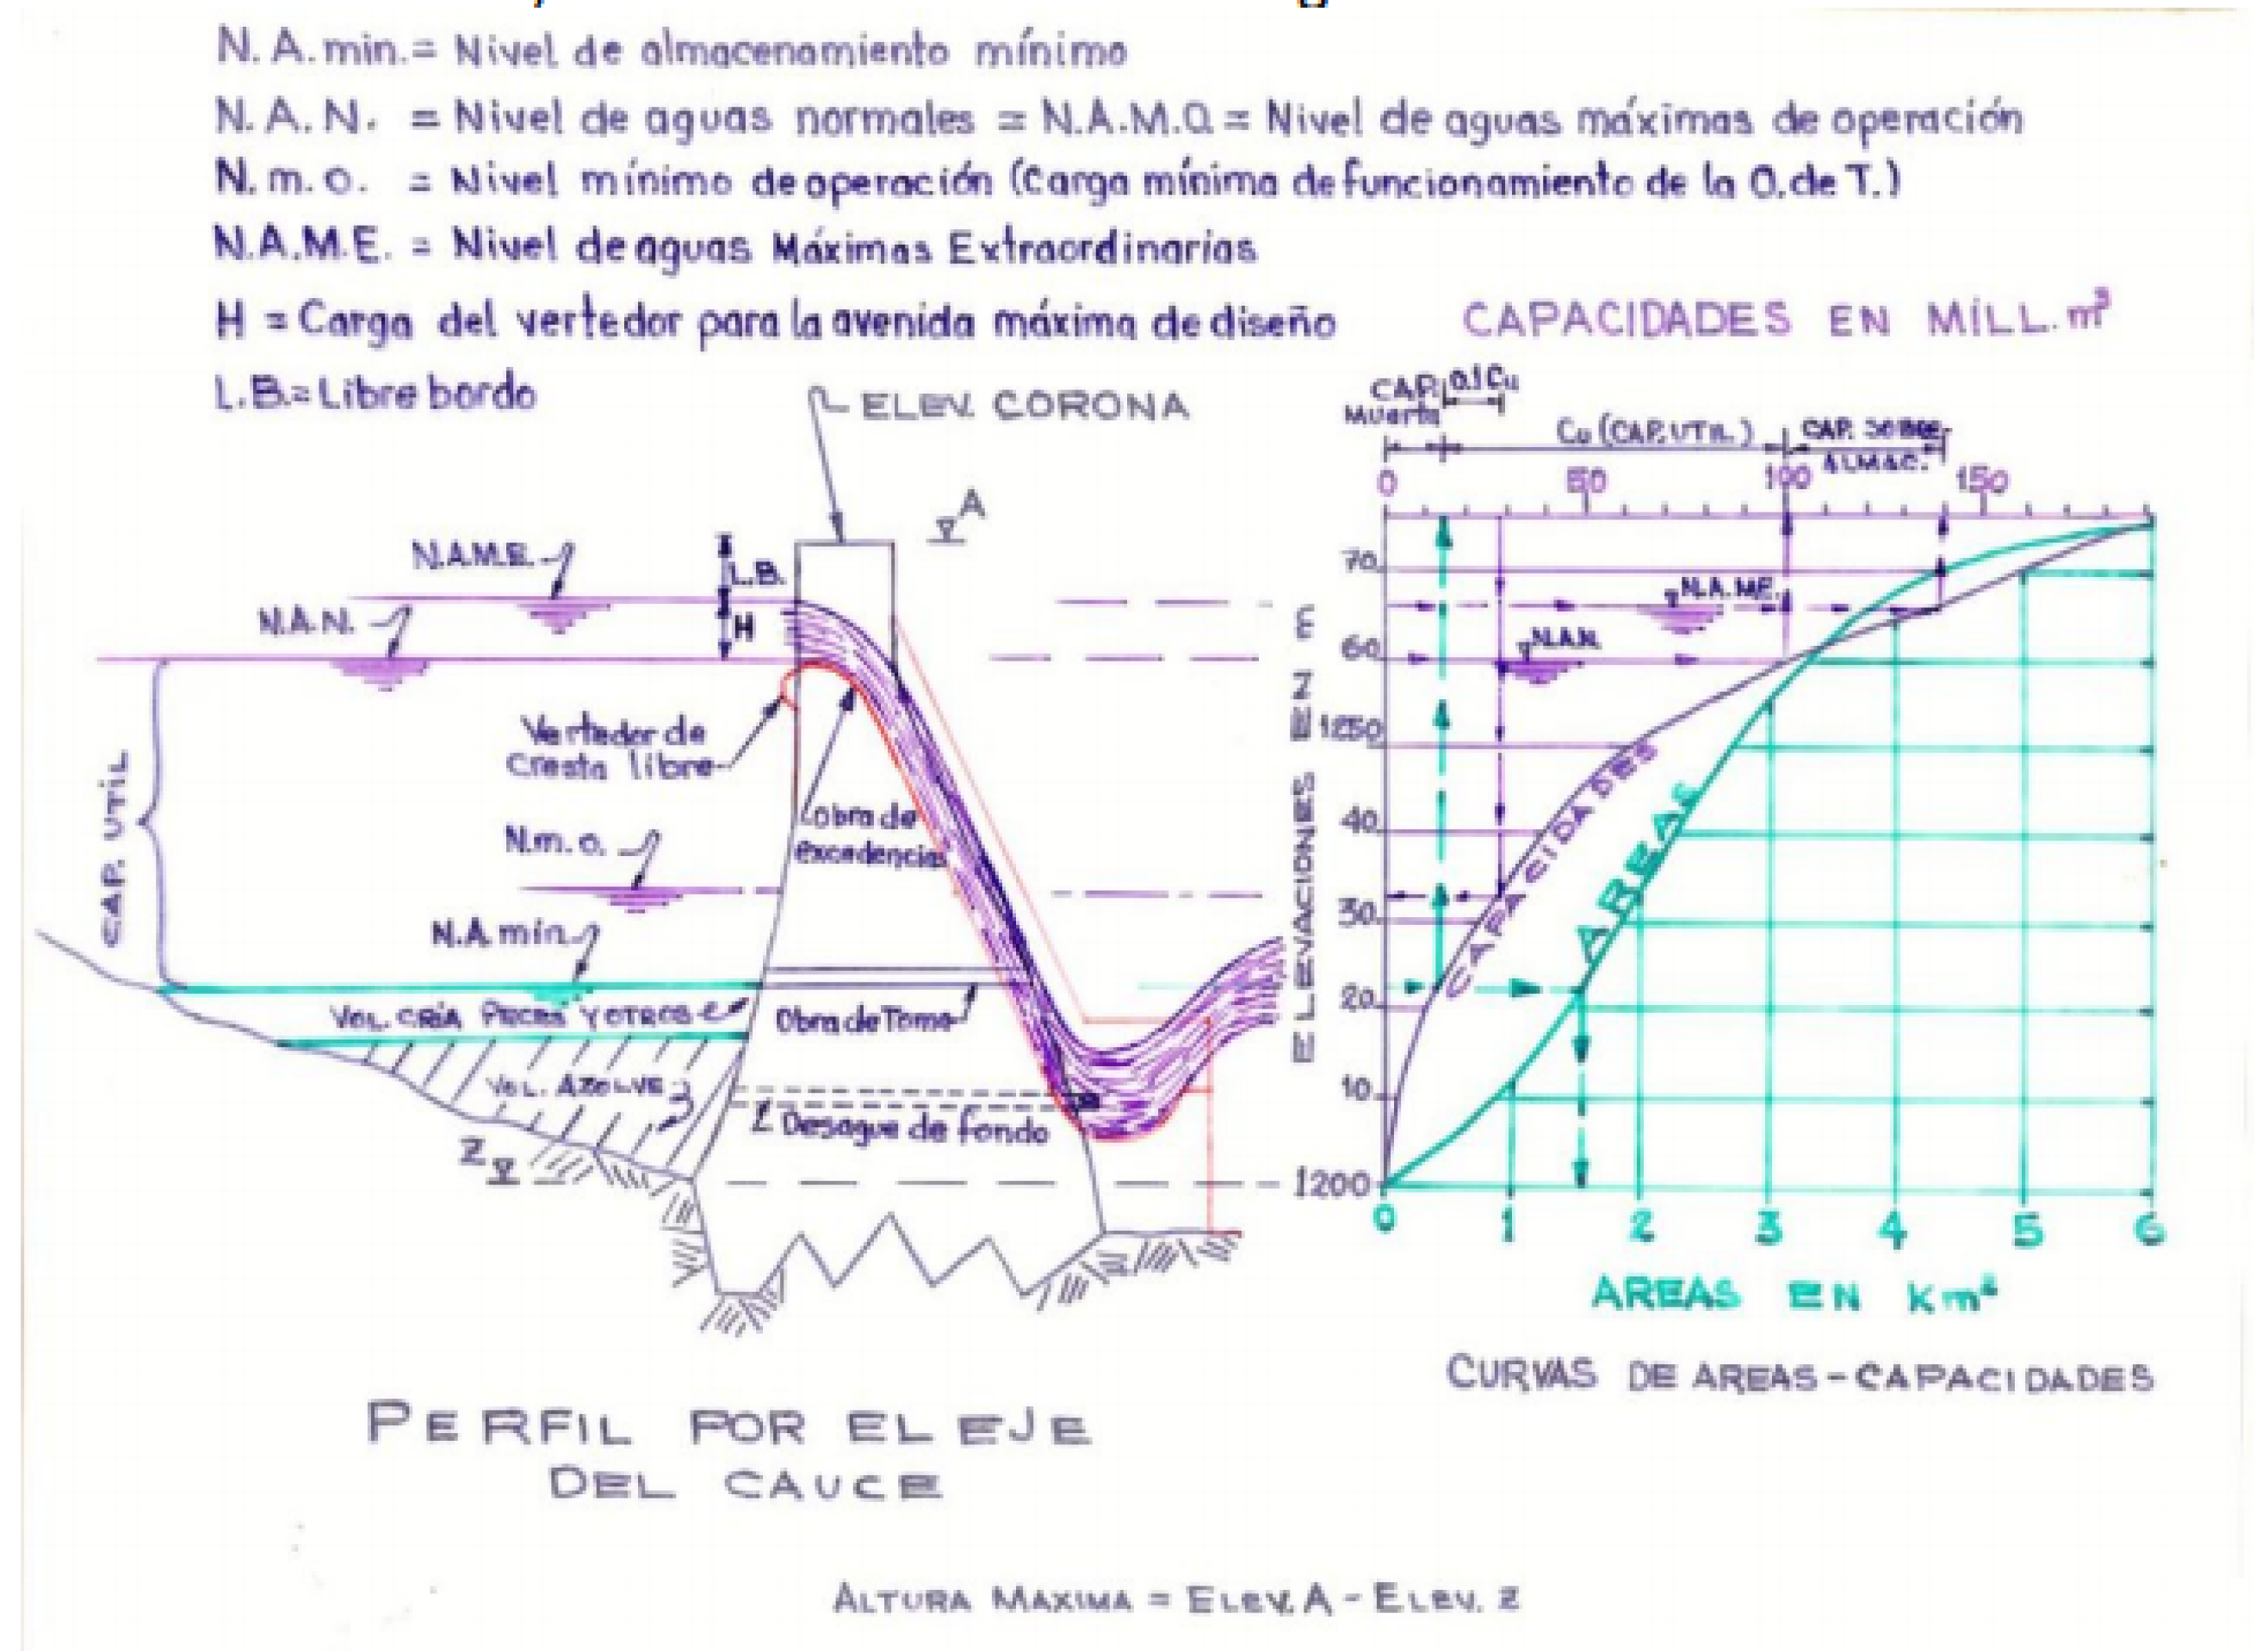
\includegraphics[width=0.5\textwidth]{fii27.png}}
			            \caption{Niveles y capacidades de almacenamiento en una presa.}
			            \label{fii27}
		            \end{figure}
		      \item \textbf{La Capacidad Útil \textbf{(Cu)}}, es el volumen de almacenamiento que representa la
		            diferencia que se tiene en un almacenamiento entre la Capacidad Total y la Capacidad
		            Muerta, este volumen queda conformado por el que se ubica entre los Niveles de
		            Aguas Normales (N.A.N.) y el Nivel de Aguas mínimo (N.A.mín.), y se integra con el
		            volumen útil que se deja para satisfacer lo beneficios que se presentan aguas abajo del
		            almacenamiento, así como el volumen de pérdidas por evaporación y de infiltración.
		      \item \textbf{La capacidad de sobre almacenamiento} es el volumen temporal del
		            almacenamiento que queda por arriba del vertedor de demasías y que se encuentra
		            comprendido entre el Nivel de Aguas Normales (N.A.N.) hasta el Nivel de Aguas
		            Máximas Extraordinarias (N.A.M.E.), esta capacidad en el vaso es de un
		            almacenamiento temporal, en tanto es desalojada por la obra de excedencias cuando
		            esta es de descarga libre, cuando esta descarga se controla por medio de compuertas
		            es un almacenamiento que se maneja acorde a los beneficios y finalidad del
		            almacenamiento, que entre otros es el control de avenidas.
		      \item \textbf{El Nivel de Aguas Máximas Extraordinarias \textbf{(N.A.M.E.)}} es la cota virtual del
		            almacenamiento que define el diseño de la obra de excedencias y que permite el paso
		            de la avenida máxima que llega al vaso y que es desalojada por esta estructura.
		      \item \textbf{El Nivel mínimo de operación \textbf{(N.m.o.)}} es la cota del almacenamiento a partir
		            del cual el gasto normal para riego es extraído en forma controlada a través de la Obra
		            de Toma y es el nivel que permite el diseño de esta estructura. Cuando se refiere el
		            N.m.o. a la operación de una máquina hidráulica (Planta de Bombeo o Instalaciones de
		            Turbinas generadoras de energía), esta cota es vital ya que es la que permite
		            operarlas, ya que si se da esta por debajo de ella se presentara un fenómeno que
		            destruiría a la máquina hidráulica, esto es el fenómeno de cavitación.
	      \end{enumerate}
	\item \textbf{Altura Máxima de la cortina:} La altura de la presa es determinada mediante la diferencia de elevaciones entre
	      la cota de la corona en la presa y la cota del fondo del cauce en la sección máxima de
	      la cortina. La elevación de la corona se obtiene con el N.A.M.E. adicionando el Libre
	      Bordo (L.B.) que es una altura de seguridad ante la presencia del oleaje que bajo la
	      acción del viento en el vaso de almacenamiento se presenta, complementado con un
	      factor de seguridad por el efecto de rompimiento de la ola al chocar con el paramento
	      mojado.
\end{enumerate}

\subsection{Obra de Retención o cortina}

\begin{definition}[Obra de retención]
	La obra de retención o cortina es la estructura del sistema de almacenamiento,
	mediante la cual se cierra artificialmente un vaso o valle natural en una cuenca de
	drenaje con el objeto de provocar un embalse. La función de esta es retener las aguas para
	formar el vaso de almacenamiento y regular los escurrimientos del cauce.
\end{definition}

Propósitos y características de una obra de retención o cortinas:
Los propósitos de una cortina son el almacenar agua para utilizarla en diferentes
usos:

\begin{itemize}
	\item  Riego
	\item  Generación de energía
	\item  Control de avenidas
	\item  Usos domésticos
	\item  Abrevadero y cría de peces
	\item  Recreación
\end{itemize}

Las características de una cortina deben brindar condiciones para que sea
Estable e Impermeable. Sus formas de clasificación de las cortinas:
\begin{enumerate}
	\item Por su uso
	      \begin{enumerate}
		      \item Generación de energía
		      \item Agua potable
		      \item Control de avenidas
		      \item Riego
	      \end{enumerate}
	\item Por su altura, están en la tabla \ref{tab17}
	      \begin{table}[h!]
		      \centering
		      \begin{tabular}{|c|c|c|c|}
			      \hline
			                & Según Torres H.        & Según U.S.B.R. & Según I.C.O.L.D. \\ \hline
			      Bajas:    & $H < 30 m$             & $H \leq 30 m$  & $H \geq 15 m$    \\ \hline
			      Medianas: & $30 m  \leq H < 100 m$ & $H \leq 90 m$  &                  \\ \hline
			      Altas:    & $H \geq 100 m$         & $H > 90 m$     & $H > 15 m$       \\ \hline
		      \end{tabular}
		      \caption{Altura de cortinas}
		      \label{tab17}
	      \end{table}
	      pueden ser Vertedoras o No vertedoras
	\item Por su funcionamiento hidráulico
	      pueden ser Vertedoras o No vertedoras
	\item Por el tipo de construcción y materiales que le constituyen.
	      pueden ser \textbf{Rígidas (Concreto
		      o Mampostería)} pero también \textbf{Flexibles ( Tierra, Enrocamiento, Materiales graduados, Madera y/o Mixtas)}
	\item Por los esfuerzos que transmiten.
	      \begin{enumerate}
		      \item En planos verticales (hacia la cimentación): Gravedad ó Machones y contrafuertes.
		      \item En planos horizontales (hacia las laderas): Arco ó Bóveda
		      \item En planos combinados (Horizontales y verticales): Arco gravedad
	      \end{enumerate}
\end{enumerate}

\subsubsection{Clasificación SRH de cortinas}
\Schema{-1.4ex}{30ex}
{\schemabox{Cortinas}} { \Schema{-1ex}{12ex}
	{\schemabox{Rígidas vertedoras\\ y no vertedoras}}
	{ \schema
		{\schemabox{Gravedad}}
		{\schemabox{Eje Recto\\ Eje Curvo\\
				Aligeradas}}
		\medskip
		\schema
		{\schemabox{Arco}}
		{\schemabox{Arco Simple\\ Arco Gravedad\\
				Bóvedas\\ Arcos Múltiples.}}
		\Schema{0ex}{3.4ex}
		{\schemabox{Diques\\ huecos}}
		{
			\Schema{0ex}{3.4ex}
			{\NudgeSB\schemabox{Losa y contrafuerte\\ Machones de cabeza\\ Bóvedas Múltiples}}
			{\schemabox{Redonda\\ Diamante}}
		}
	}
	\Schema{-1ex}{5ex}
	{\schemabox{Flexibles}}
	{
		\vskip1ex\schemabox{Materiales graduados}
		\medskip
		\schemabox{Tierras (Homogéneas)}
		\medskip
		\schema
		{\schemabox{Enrocamiento}}
		{\schemabox{Con Corazón Impermeable\\ Con Membrana Impermeable}}
	}
	\Schema{-1ex}{5ex}
	{\schemabox{Mixtas}}
	{
		\schemabox{Madera y enrocamiento}
		\medskip\schemabox{Madera y Concreto}
		\medskip
		\schemabox{Concreto y Fierro}}
	\Schema{-1ex}{5ex}
	{\schemabox{Compuertas}}
	{
		\schemabox{Diversos Materiales en diversas secciones}}}

\subsection{Diversos tipos de presas}

\subsubsection{Cortinas o presas de gravedad:}
Es una estructura sólida de algún material rígido que se diseña y se
proporciona, para asegurar su estabilidad contra los efectos de todas las fuerzas que
se le impongan a partir del empuje del agua. Se usa la mampostería: en presas pequeñas $(H<30 m)$, este material se
conforma con piedra (o roca) junteada con mortero de cemento (mezcla cemento arena), debidamente colocada.

Otra opción, se puede usar Concreto simple, material que se conforma con una mezcla de arena, grava, cemento y agua;

La tercera opción es Concreto ciclópeo: piedra agregada en un 30\% sobre el concreto simple. Finalmente se puede optar por usar el colcreto: piedra rellenada con mortero coloidal, ya sea inyectada o
colocada por gravedad. Se le conoce como mampostería inyectada.

\subsubsection{Cortinas o presas de arco:} Es una estructura sólida construida normalmente de concreto de gran esbeltez, en forma de arco, la que, a través del efecto de este, hace que los esfuerzos originados en el empuje del agua, todos ellos vayan a dar a las laderas.

\begin{figure}[h!]
	\centerline{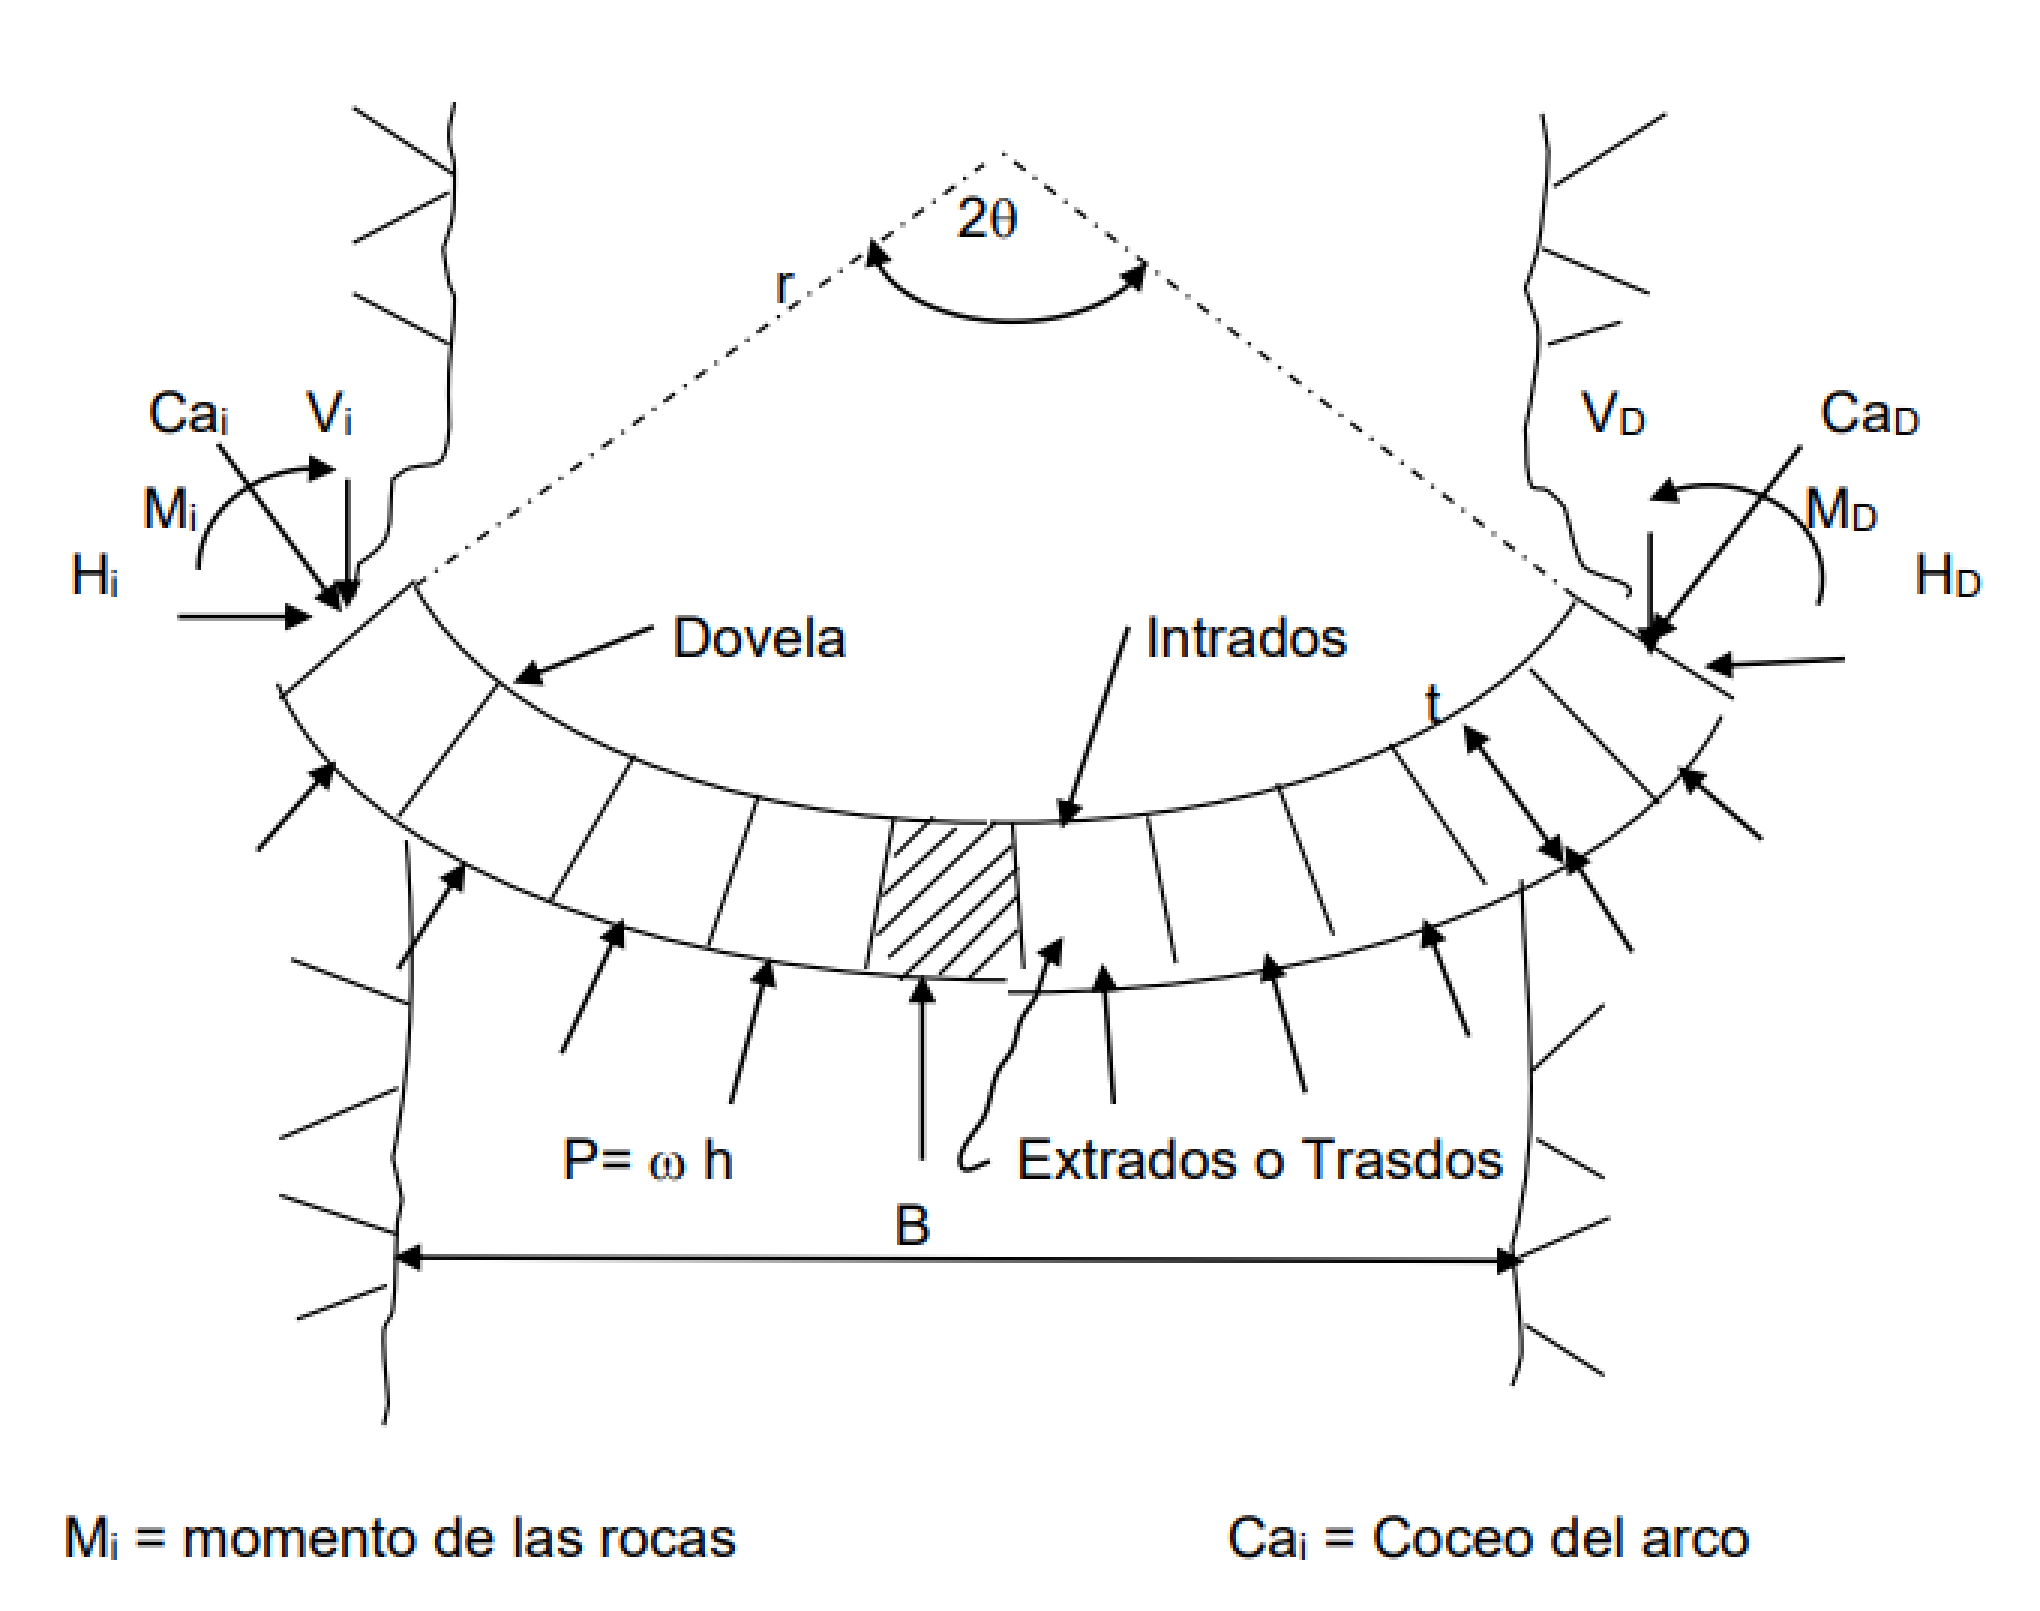
\includegraphics[width=0.5\textwidth]{fii28.png}}
	\caption{ Planta esquemática de Presa de arco.}
	\label{fii28}
\end{figure}

El Arco óptimo se tiene con: $2\theta = 133^{\circ} 34'$; Para minimizar material, los arcos se pueden encontrar entre: $100^{\circ} \leq  2\theta \leq  140^{\circ}$P
Para cañones de: $B \leq \frac{H}{3} \longrightarrow$ Presa de arco
Para cañones de: $B \geq 2.5H \longrightarrow$ Presas de Arco-Gravedad.
\begin{figure}[h!]
	\centerline{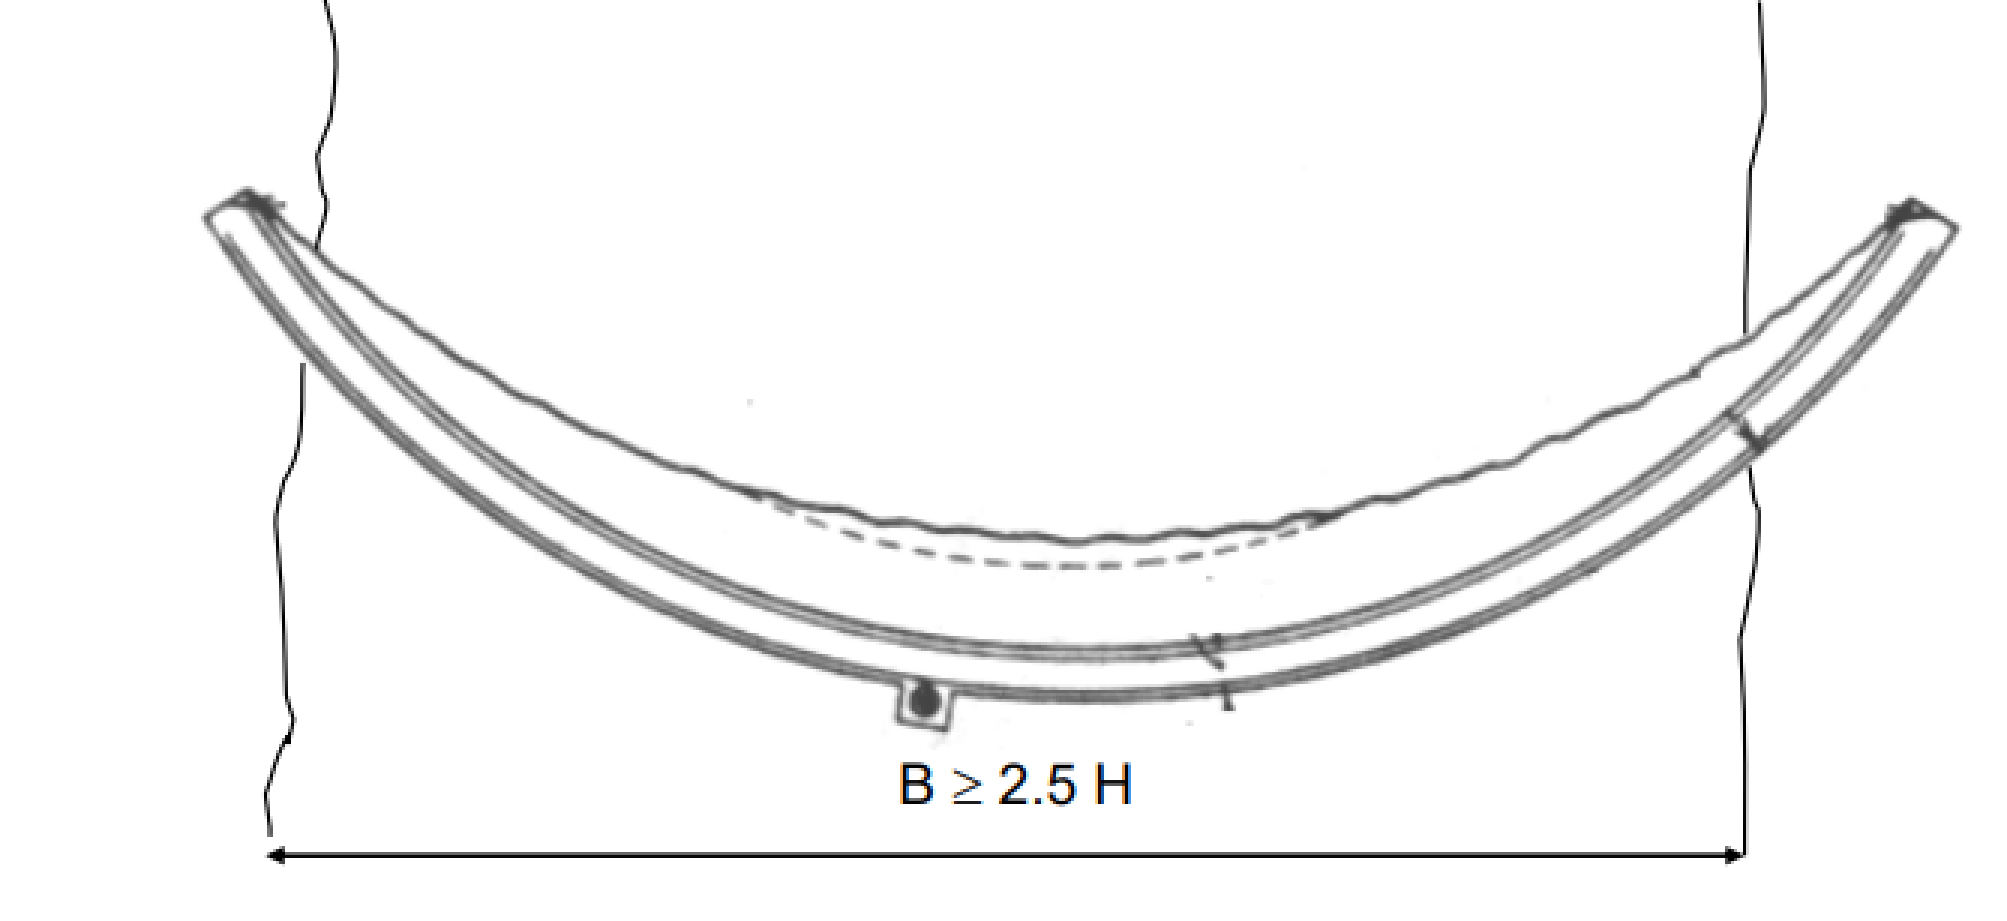
\includegraphics[width=0.5\textwidth]{fii29.png}}
	\caption{Forma en planta de una presa de arco.}
	\label{fii29}
\end{figure}
\textbf{Por su geometría:} Radio Constante o de centro constante y por Radio variable o ángulo constante
\begin{figure}[h!]
	\centerline{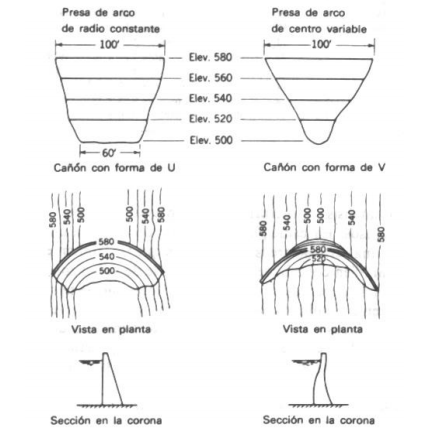
\includegraphics[width=0.5\textwidth]{fii30.png}}
	\caption{Clasificación de presas de arco.}
	\label{fii30}
\end{figure}
\textbf{Por su simetría respecto al eje del cañón:} Simétricas y Asimétricas

%%%%%%%%%%%%%%%%%%%%% Asimetría en presas de arco img


\textbf{Por su espesor:} Arco delgado $( \frac{r}{t\geq 5} )$, Arco grueso $( \frac{r}{t < 5})$, Espesor constante y Espesor variable.

\subsubsection{Cortina o presa de diques huecos:} Este tipo de presas se caracteriza por tener una membrana inclinada que
transmite la carga de agua a una serie de contrafuertes (o machones) en ángulos rectos al eje de la presa.
\begin{figure}[h!]
	\centerline{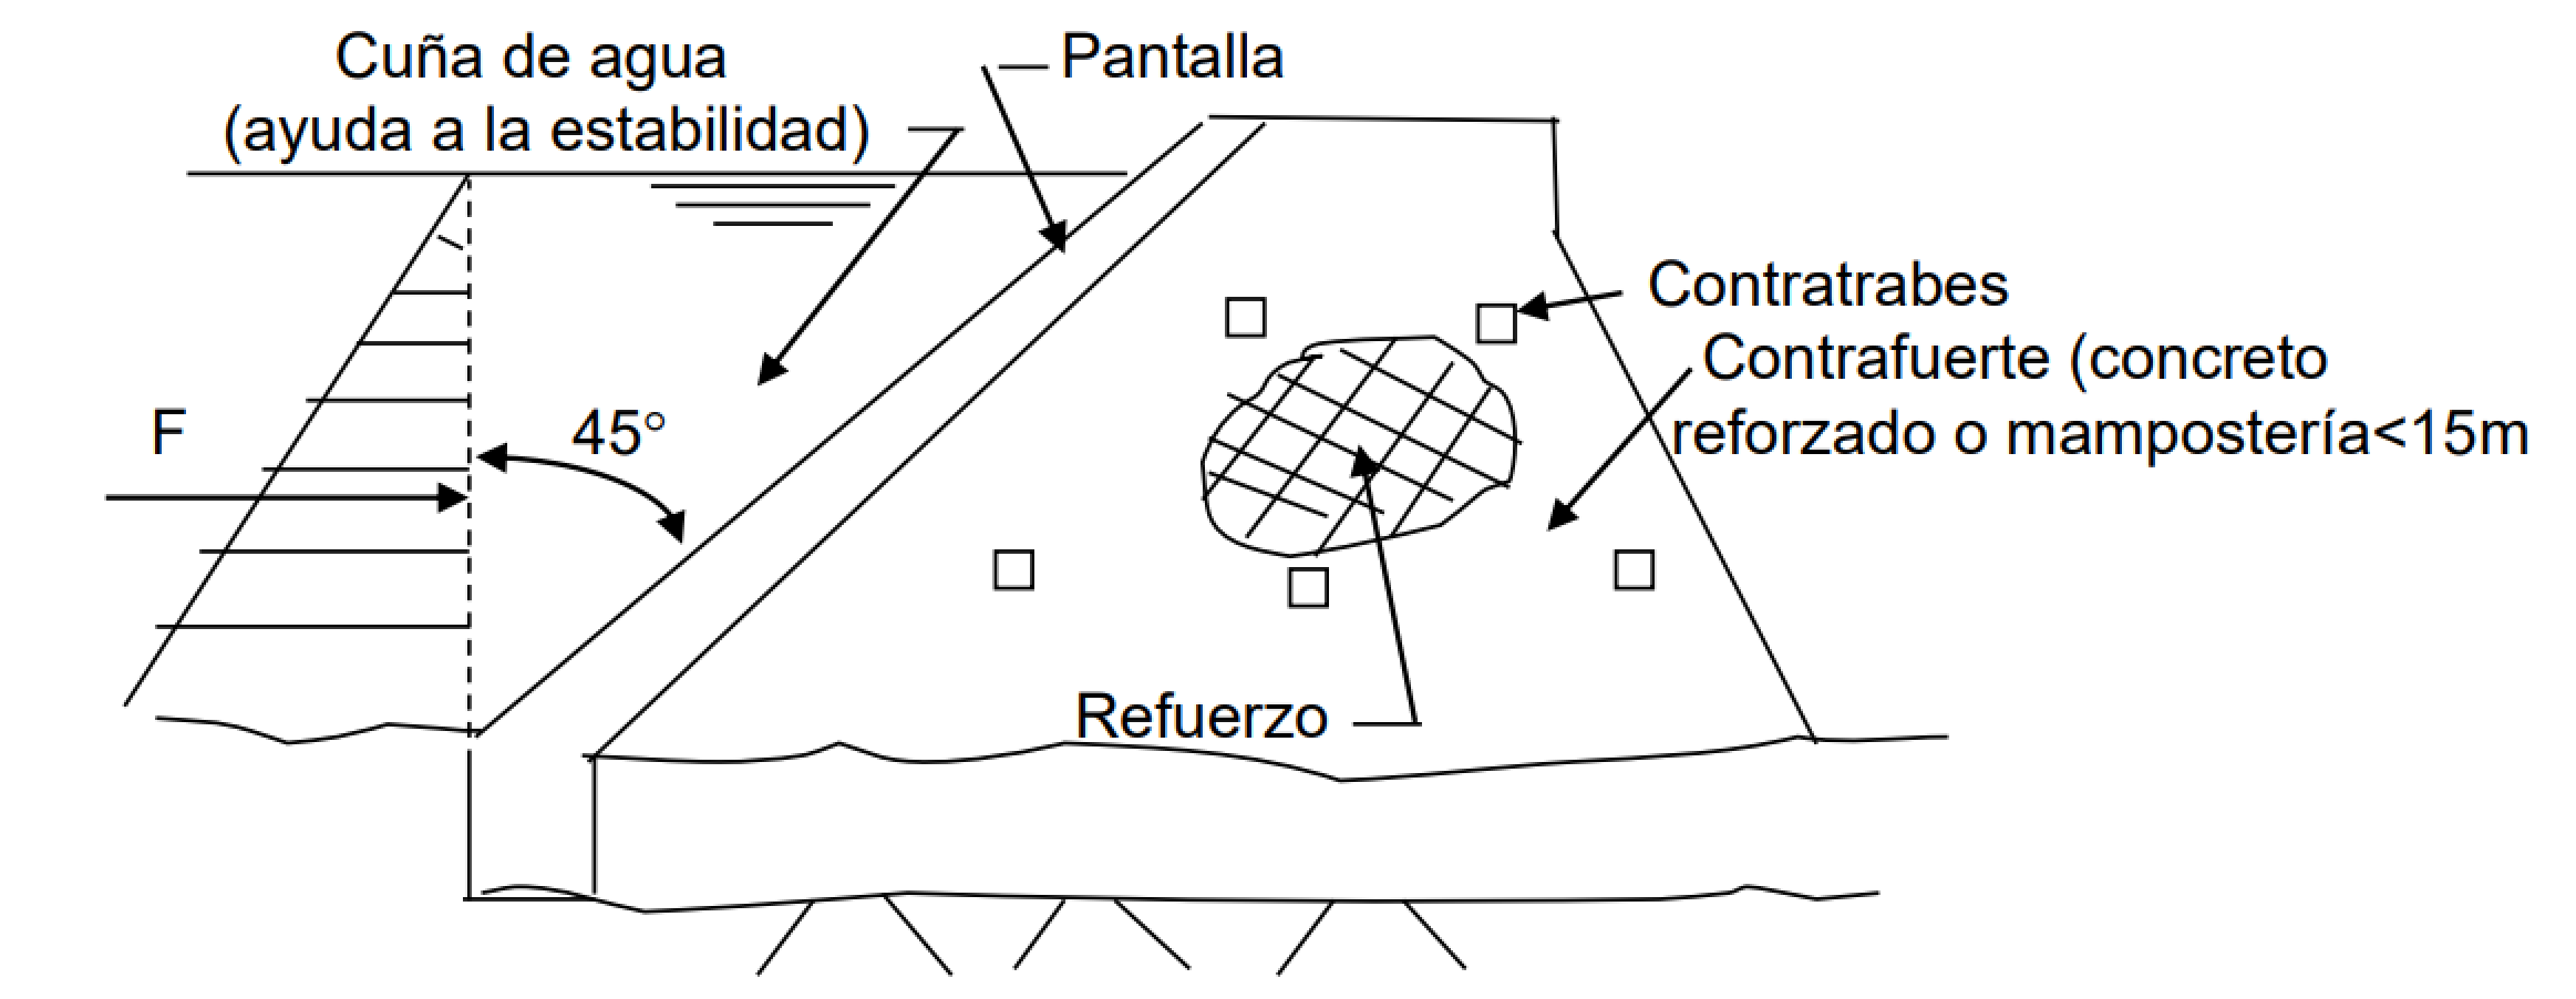
\includegraphics[width=0.5\textwidth]{fii31.png}}
	\caption{Esquema de Presa de diques huecos tipo Ambursen.}
	\label{fii31}
\end{figure}
Nils Ambursen construyó en 1903 la primera presa de machones y losa de concreto.

\begin{figure}[h!]
	\centerline{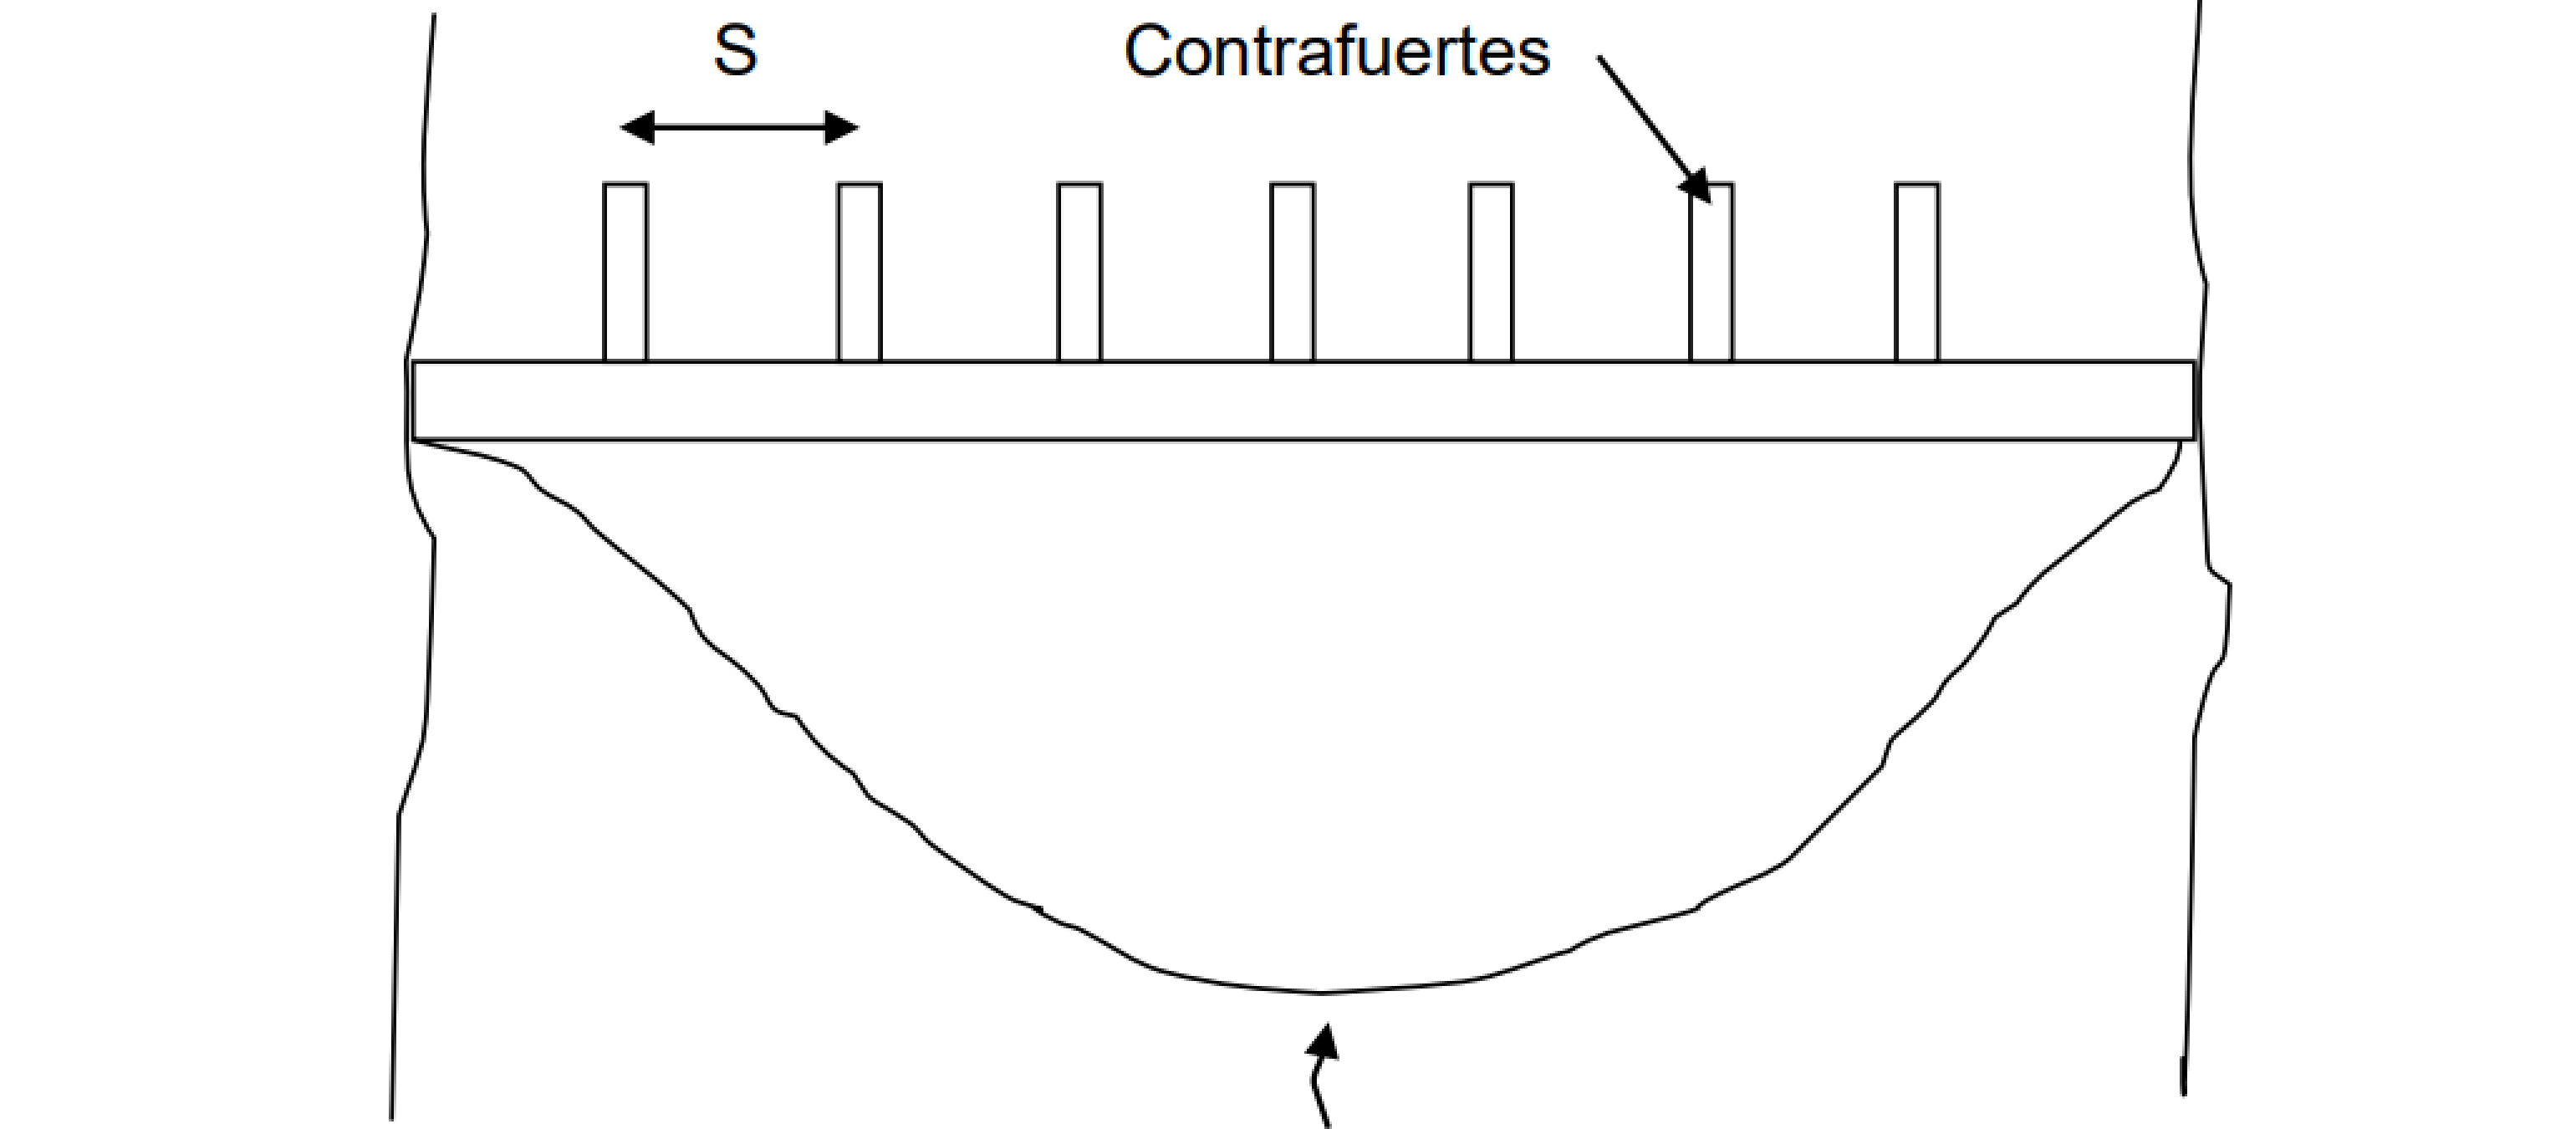
\includegraphics[width=0.5\textwidth]{fii32.png}}
	\caption{ Planta Esquemática genérica de Presa de diques huecos.}
	\label{fii32}
\end{figure}

Clasificación de Presas de diques huecos:

\begin{enumerate}[noitemsep]
	\item Pantalla y contrafuertes (Ambursen), Separación del contrafuerte:
	      $ S= 5 m \longrightarrow H= 15 m$
	      $S=15m \longrightarrow H = 50 m$
	\item Arcos múltiples $( 2\theta = 180^{\circ}, 190^{\circ})$
	\item Machones de cabeza : En T, Redonda, Diamante y Machones celulares
	\item Bóvedas múltiples:
	      \begin{figure}[h!]
		      \centerline{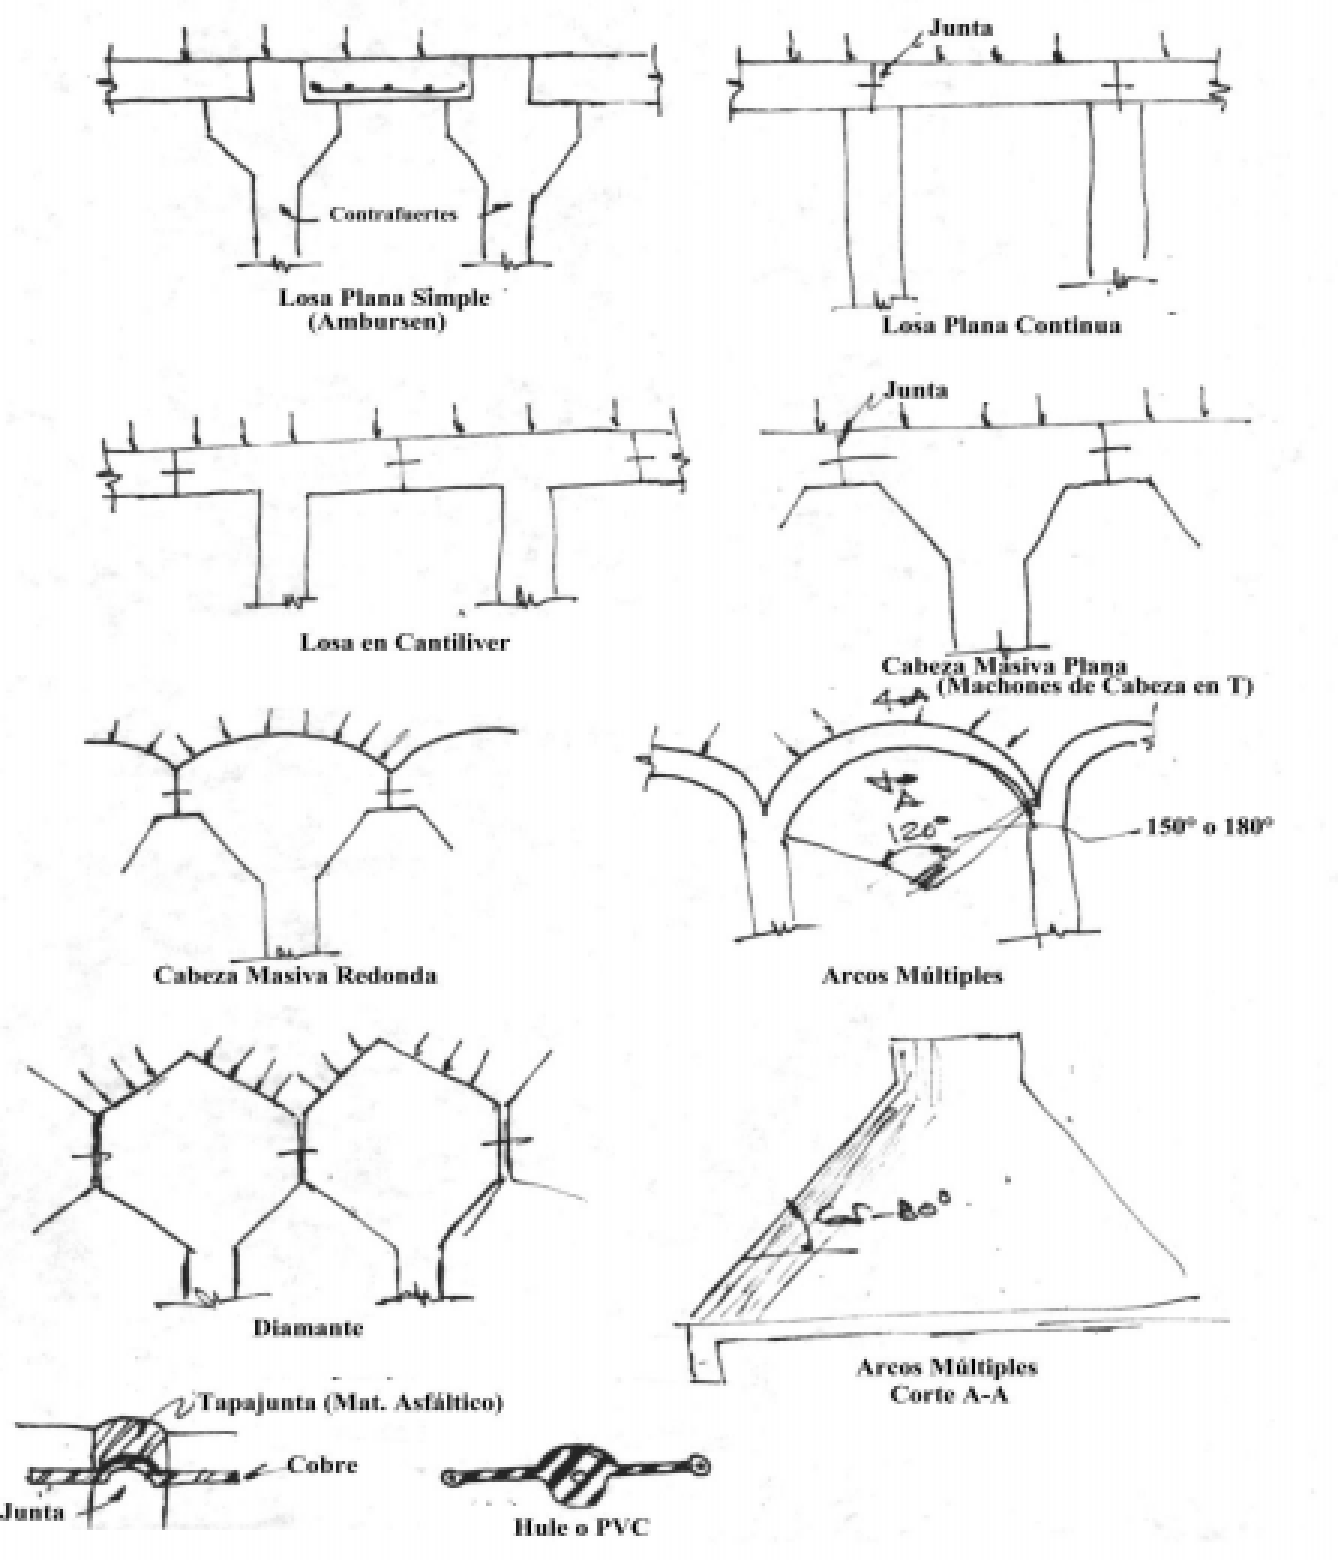
\includegraphics[width=0.5\textwidth]{fii33.png}}
		      \caption{Diferentes plantas esquemáticas de presas de diques huecos.}
		      \label{fii33}
	      \end{figure}
	      \begin{figure}[h!]
		      \centerline{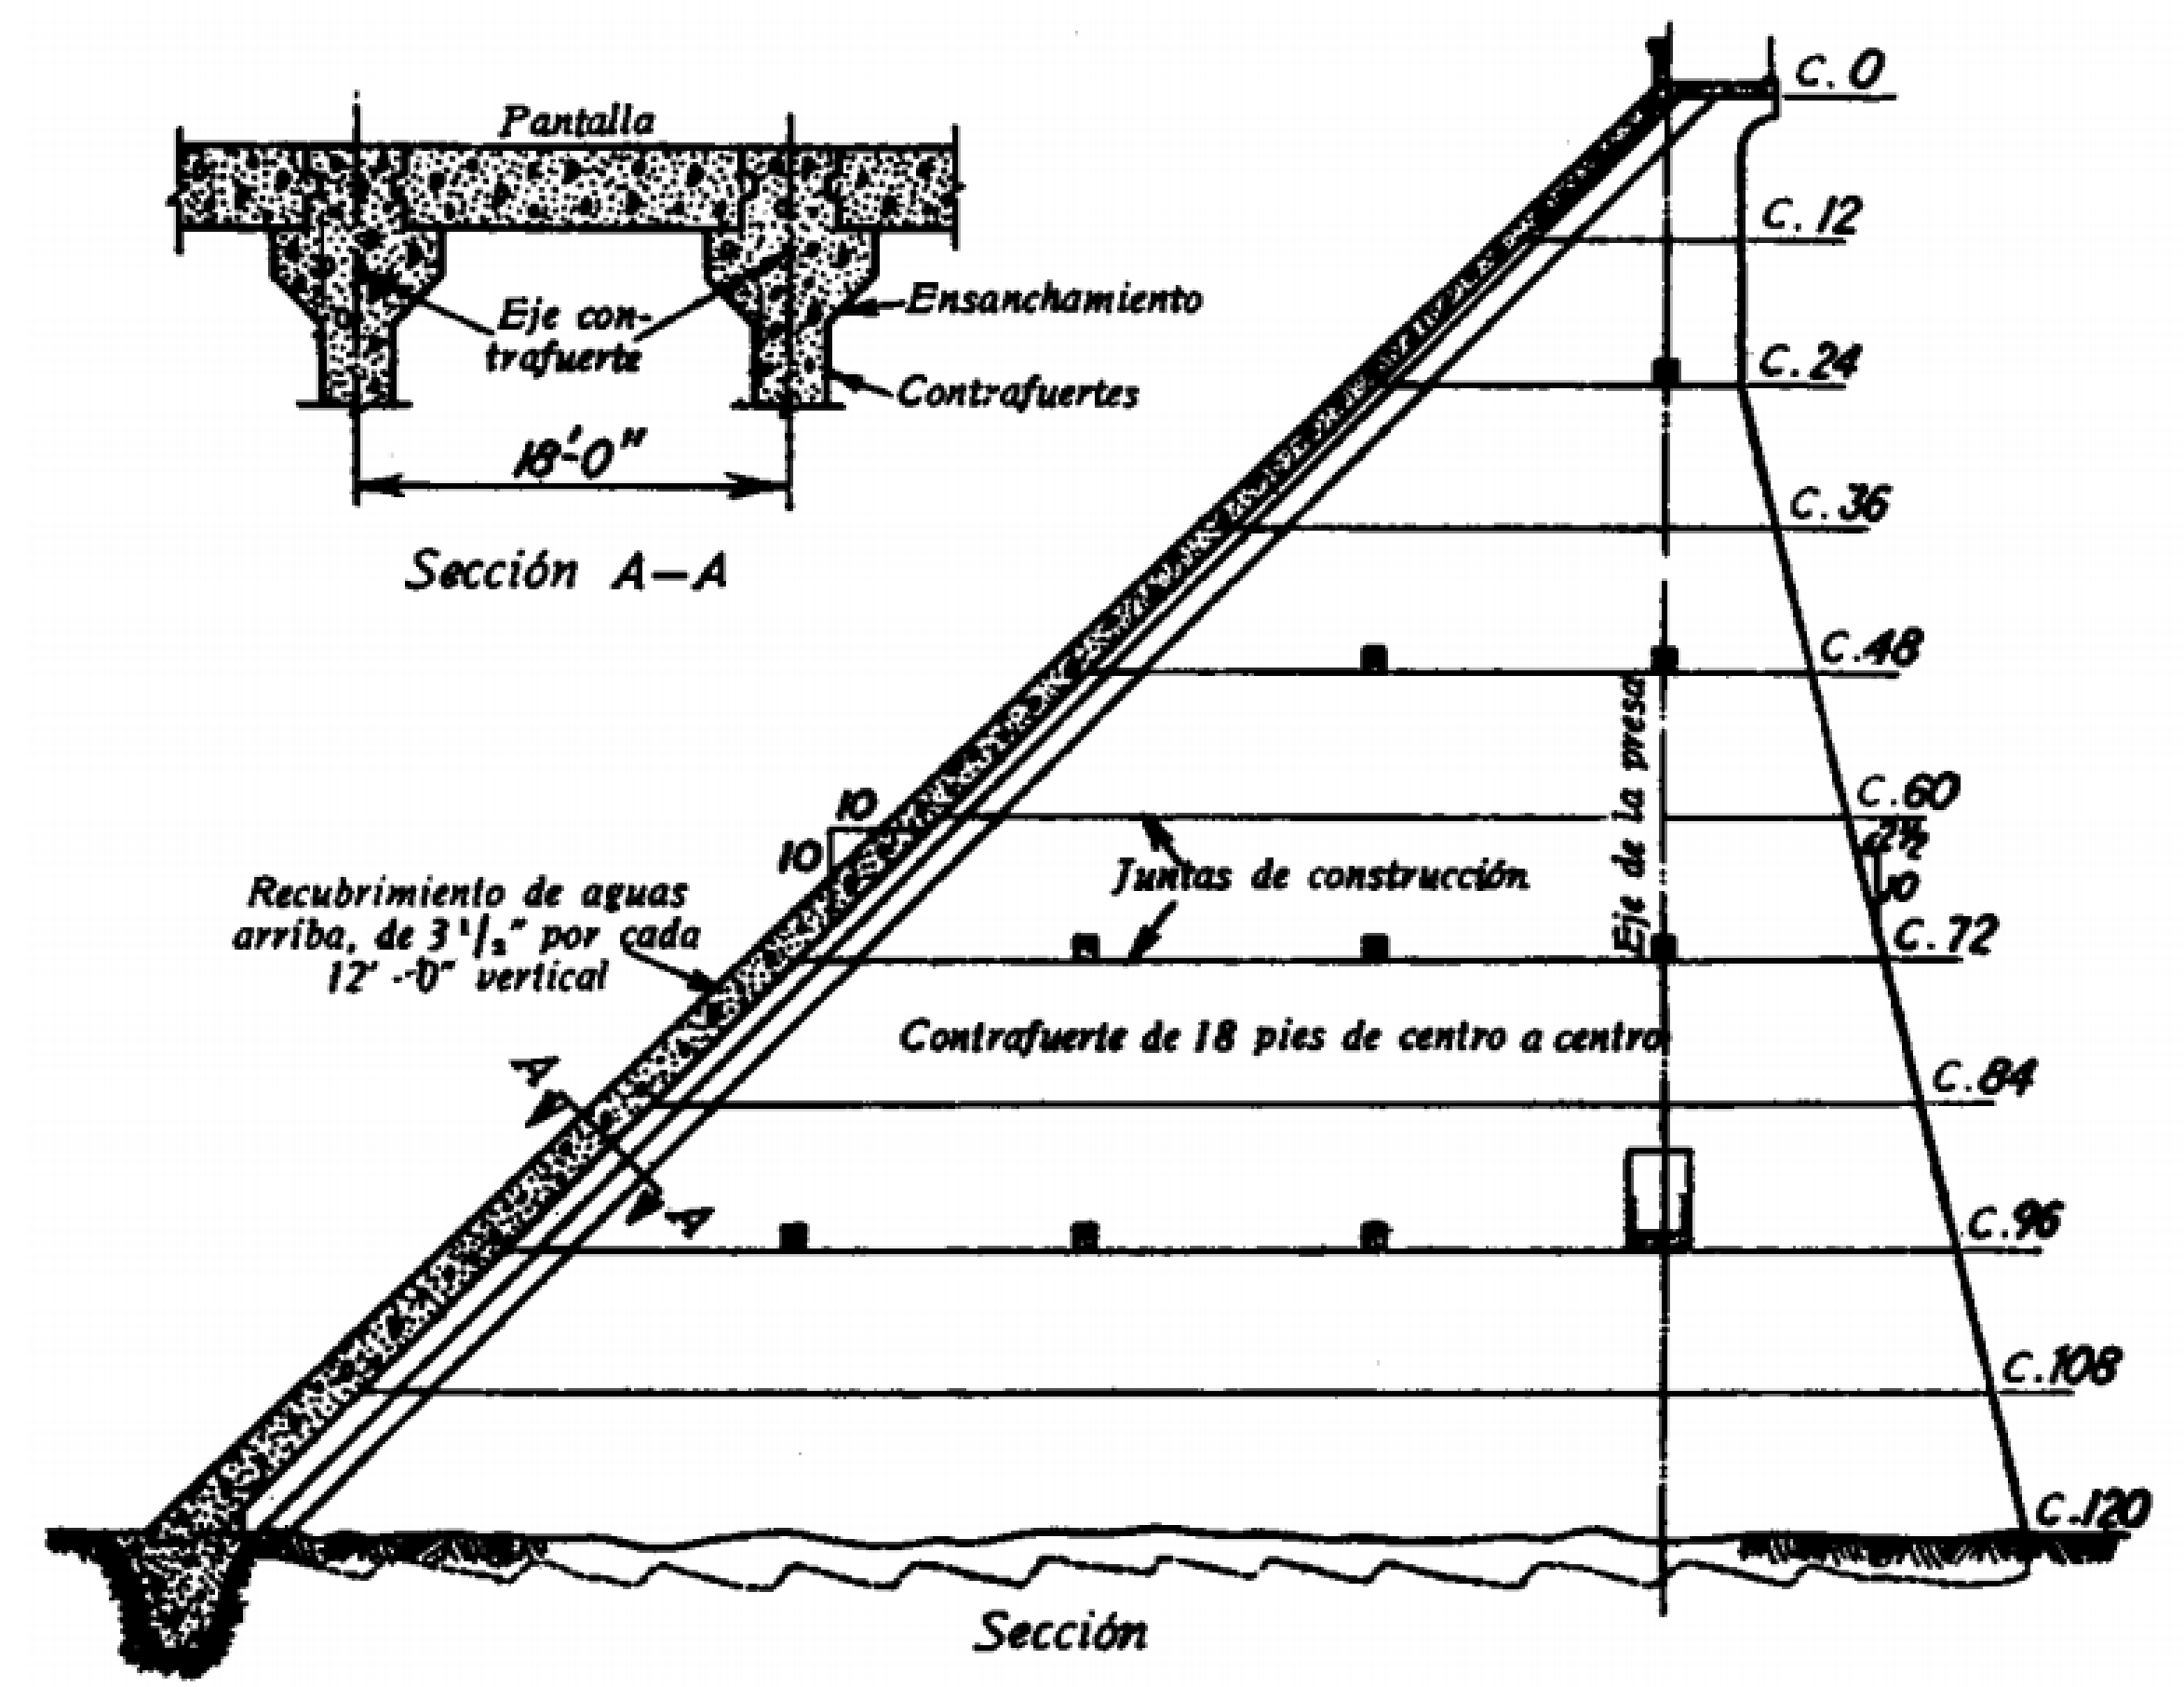
\includegraphics[width=0.5\textwidth]{fii34.png}}
		      \caption{Perfil esquemático de Presa de diques huecos tipo losa y contrafuertes.}
		      \label{fii34}
	      \end{figure}
	      \begin{figure}[h!]
		      \centerline{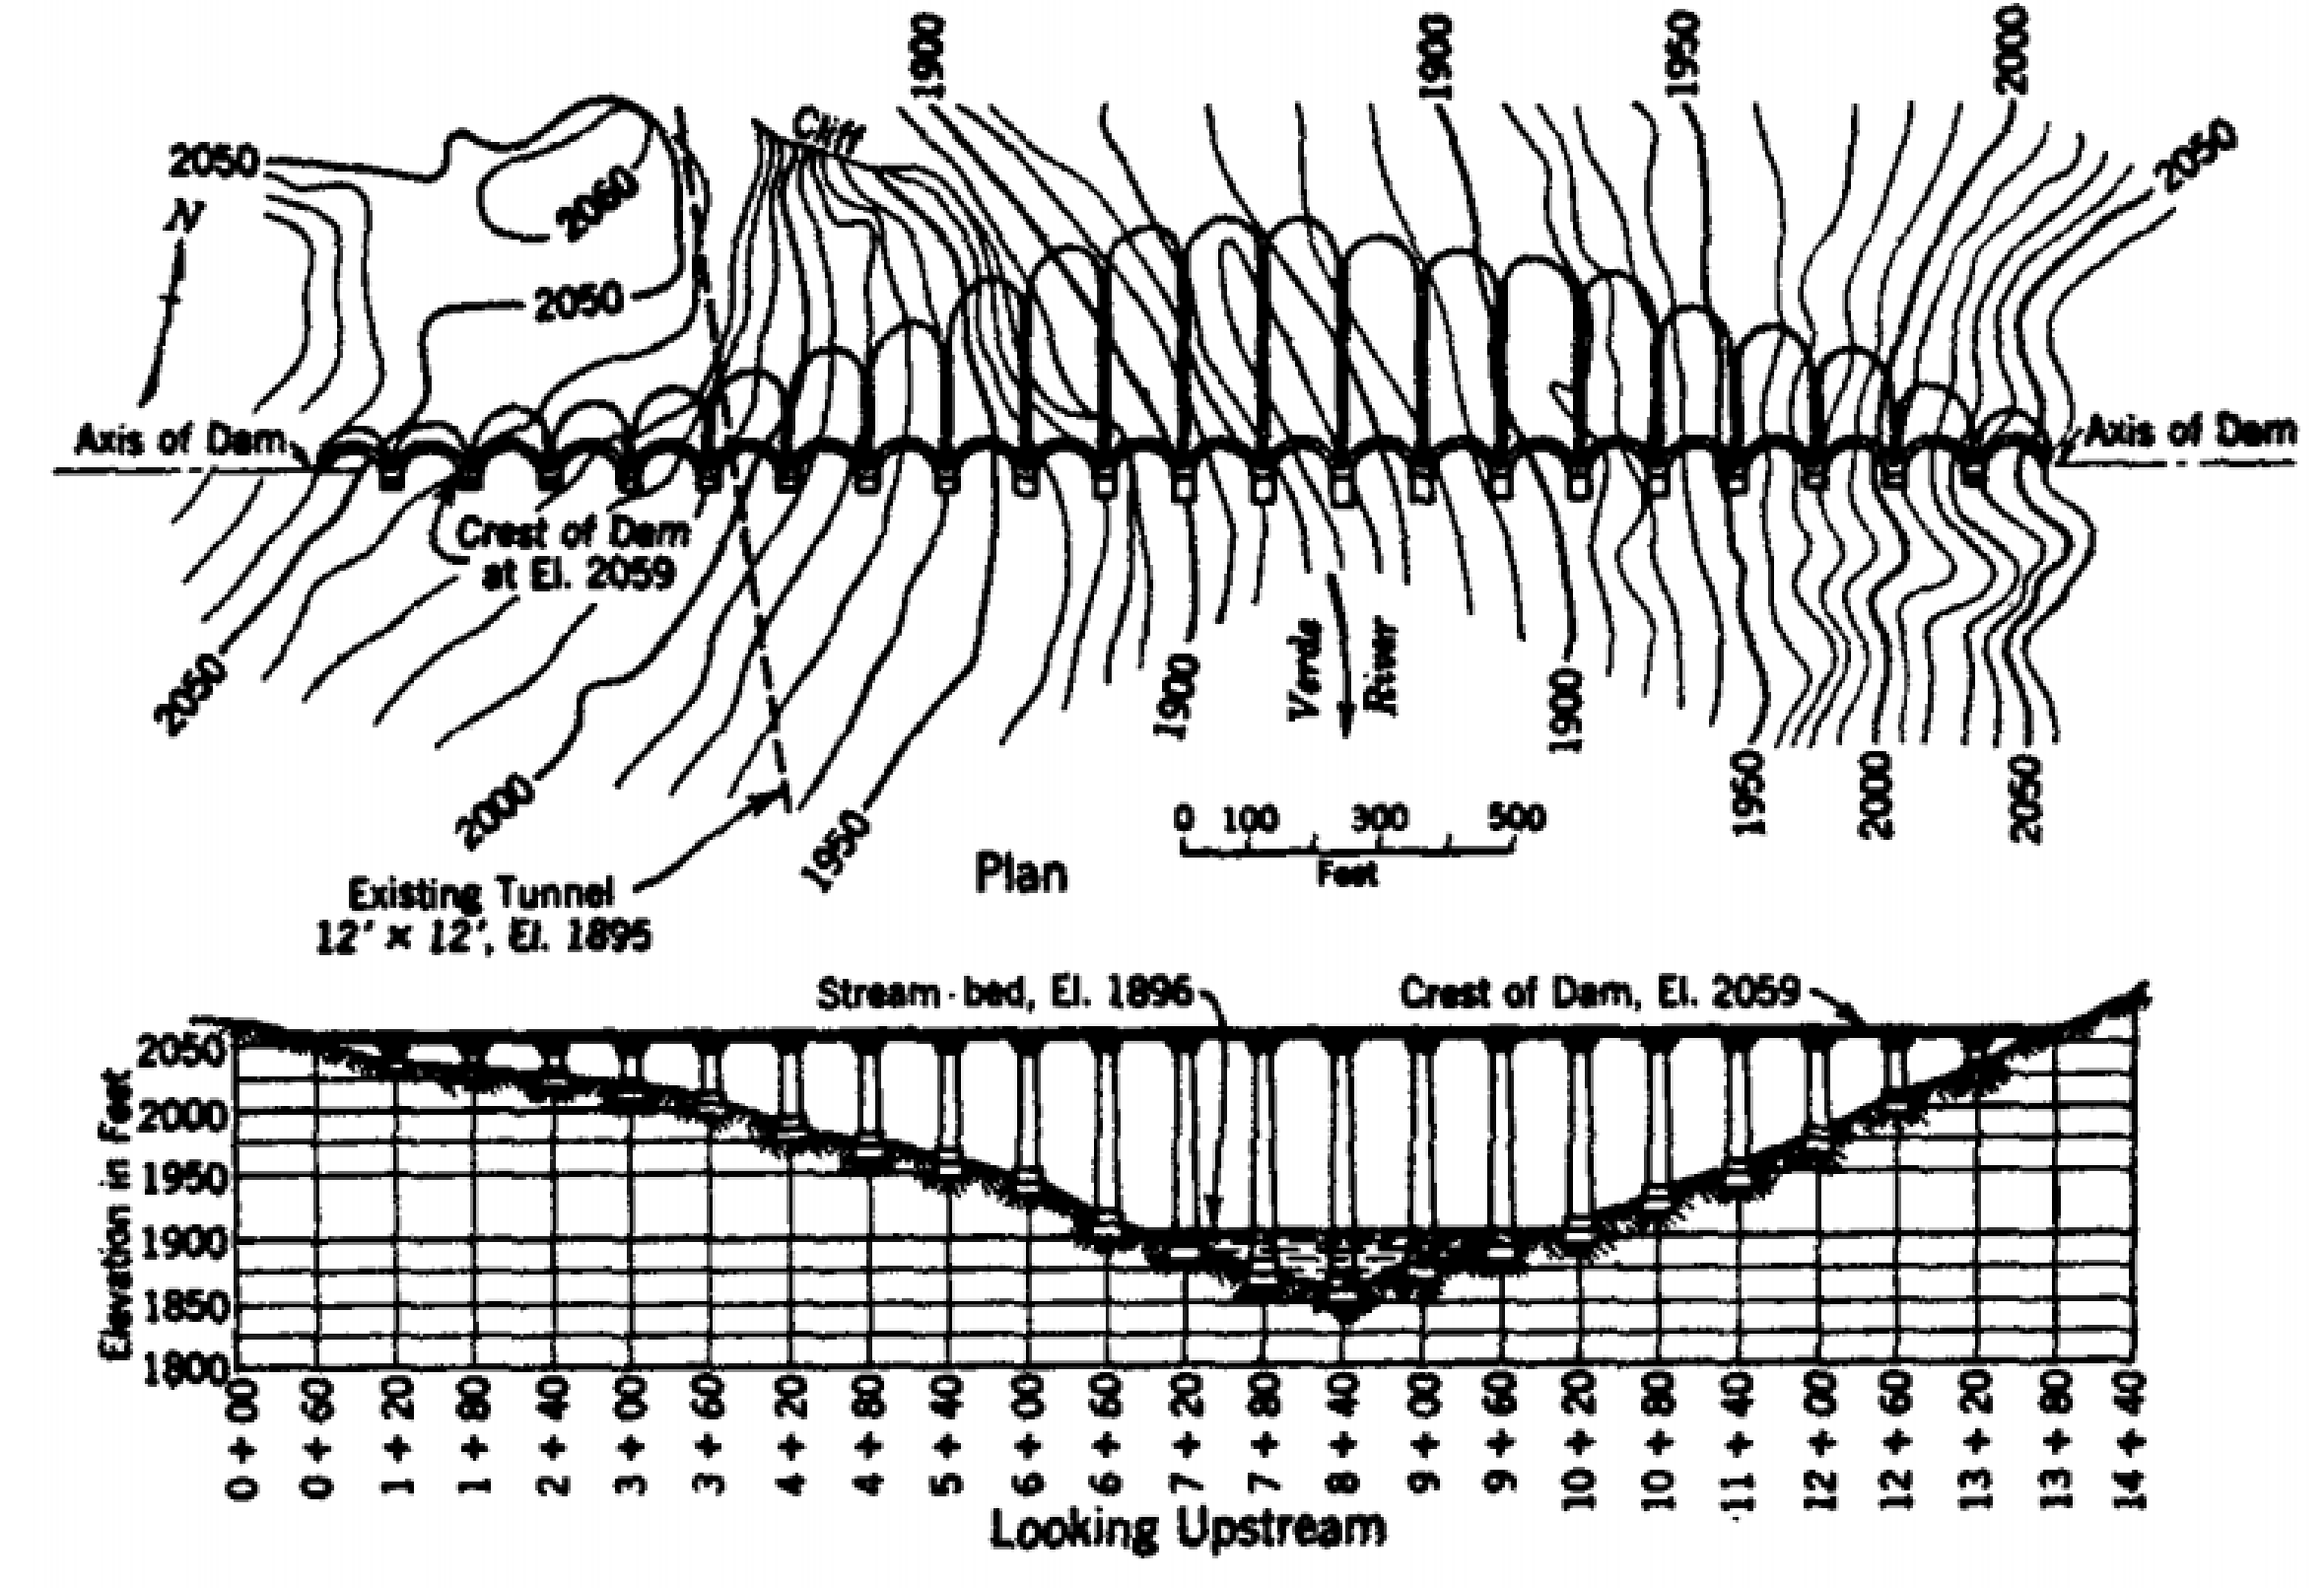
\includegraphics[width=0.5\textwidth]{fii35.png}}
		      \caption{Planta y perfil por el eje de Presa de diques huecos tipo arcos
			      múltiples.}
		      \label{fii35}
	      \end{figure}
	      \begin{figure}[h!]
		      \centerline{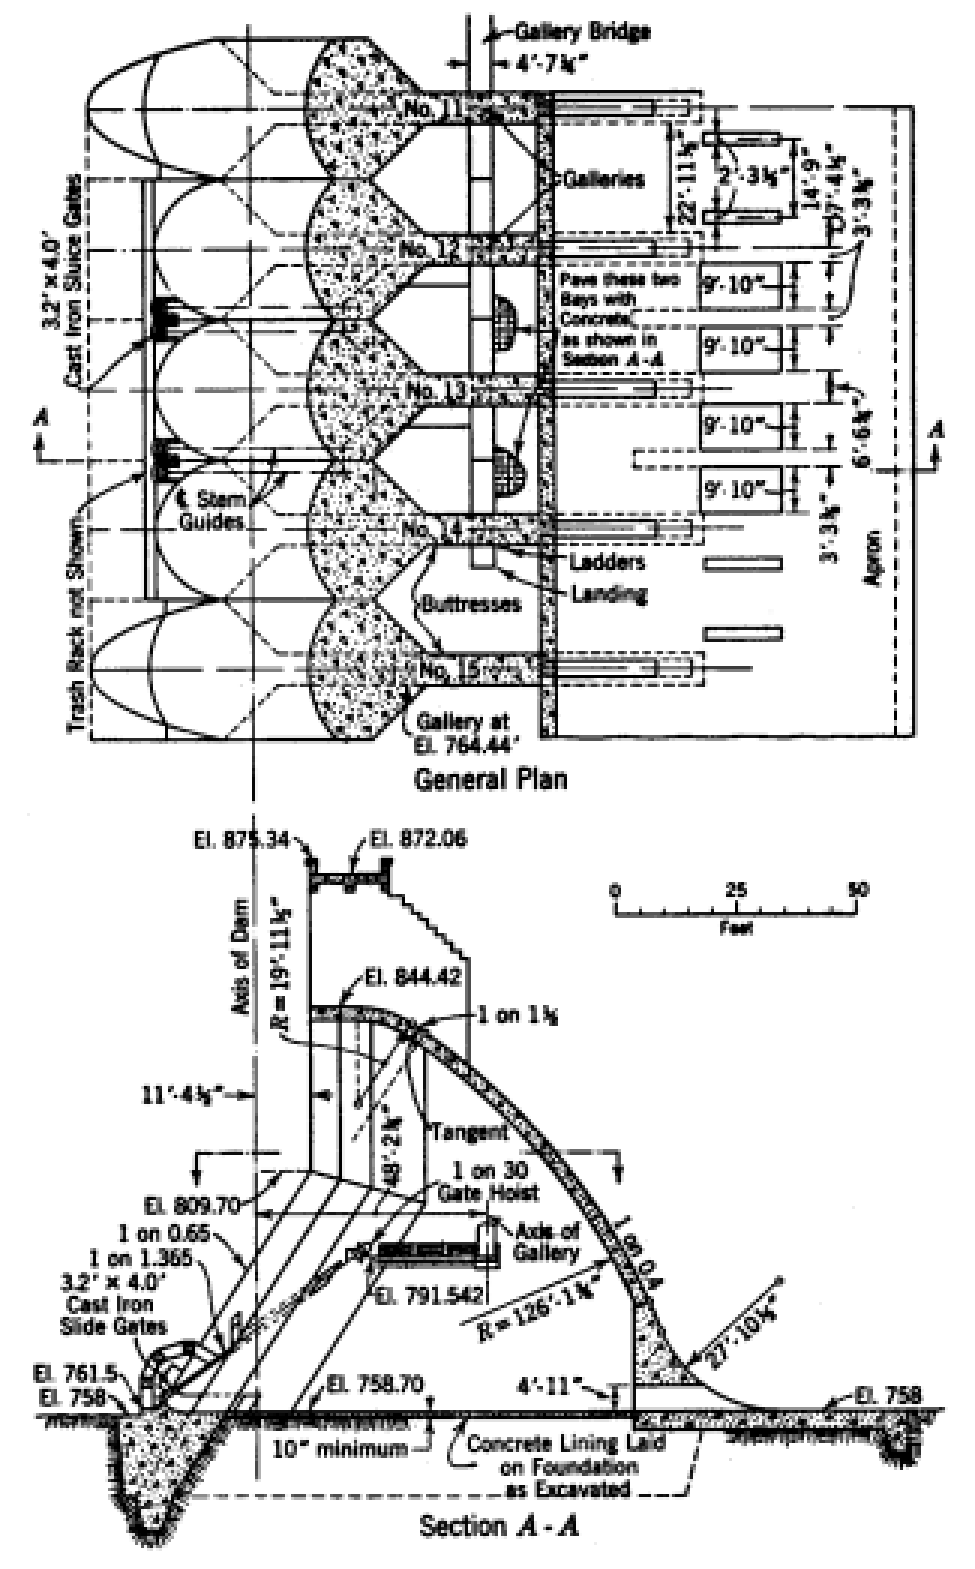
\includegraphics[width=0.5\textwidth]{fii36.png}}
		      \caption{Planta y Perfil de Presa de diques huecos tipo machones de cabeza
			      redonda.}
		      \label{fii36}
	      \end{figure}
\end{enumerate}

\subsubsection{Cortinas de materiales flexibles}

\subsubsection{Presas de tierra}

\begin{definition}[Presas de tierra]
	Una presa de tierra es una estructura formada con materiales naturales
	granulares sin más tratamiento que su colocación debidamente compactados.
\end{definition}

Secciones típicas: las Homogéneas se dividen en presas pequeñas y mixtas. Los materiales graduados se usan para las presas grandes.

\begin{enumerate}[noitemsep]
	\item Presas de tierra de sección homogénea
	      \begin{figure}[h!]
		      \centerline{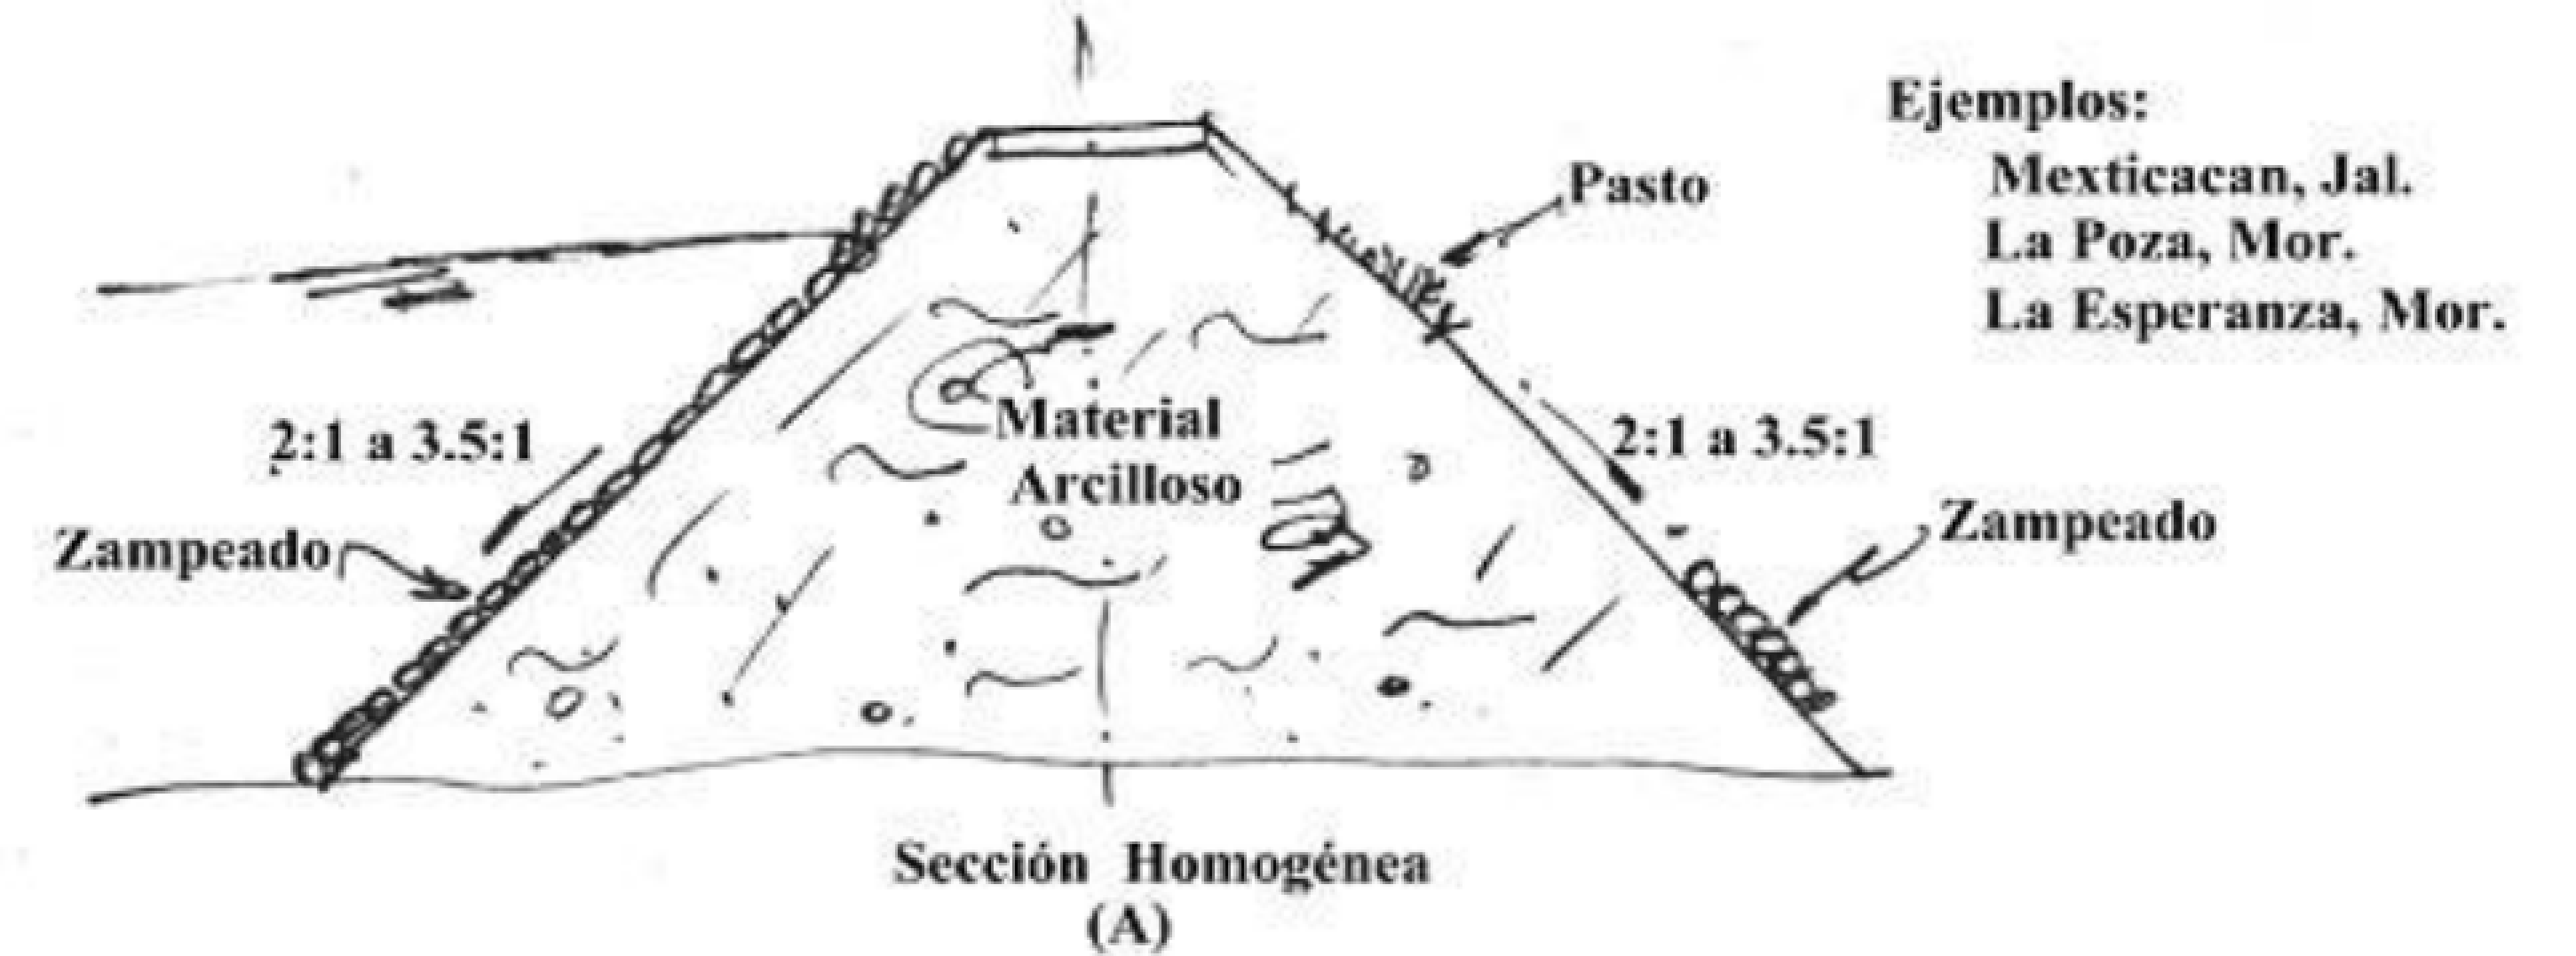
\includegraphics[width=0.5\textwidth]{fii37.png}}
		      \caption{Sección esquemática de presa de tierra tipo homogénea.}
		      \label{fii37}
	      \end{figure}
	\item Presa de tierra de sección tipo mixta.
	      \begin{figure}[h!]
		      \centerline{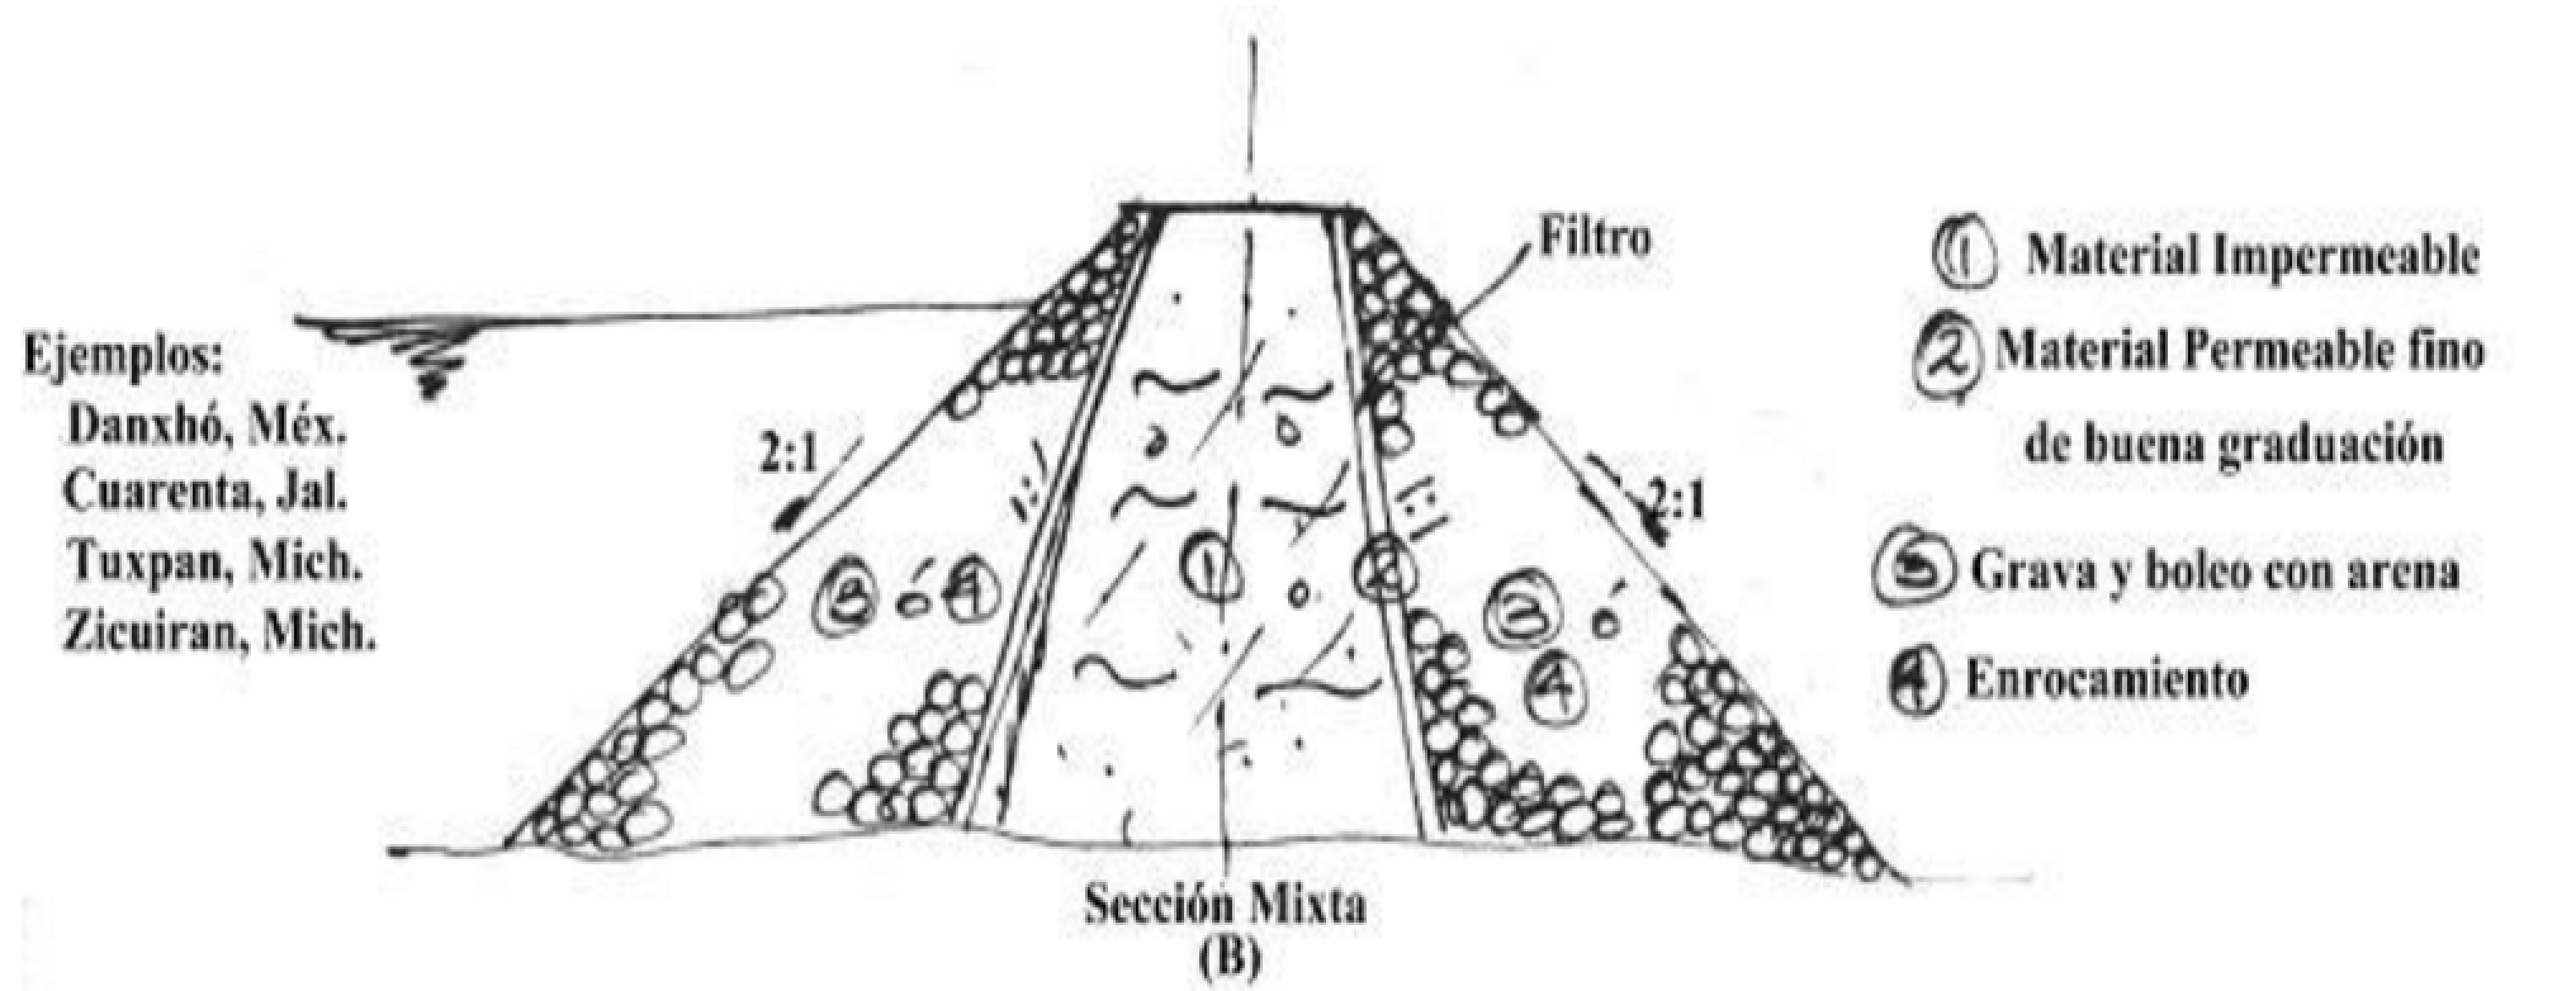
\includegraphics[width=0.5\textwidth]{fii38.png}}
		      \caption{Sección esquemática de presa de tierra tipo mixto.}
		      \label{fii38}
	      \end{figure}
	\item Presa de tierra de sección de materiales graduados
	      \begin{figure}[h!]
		      \centerline{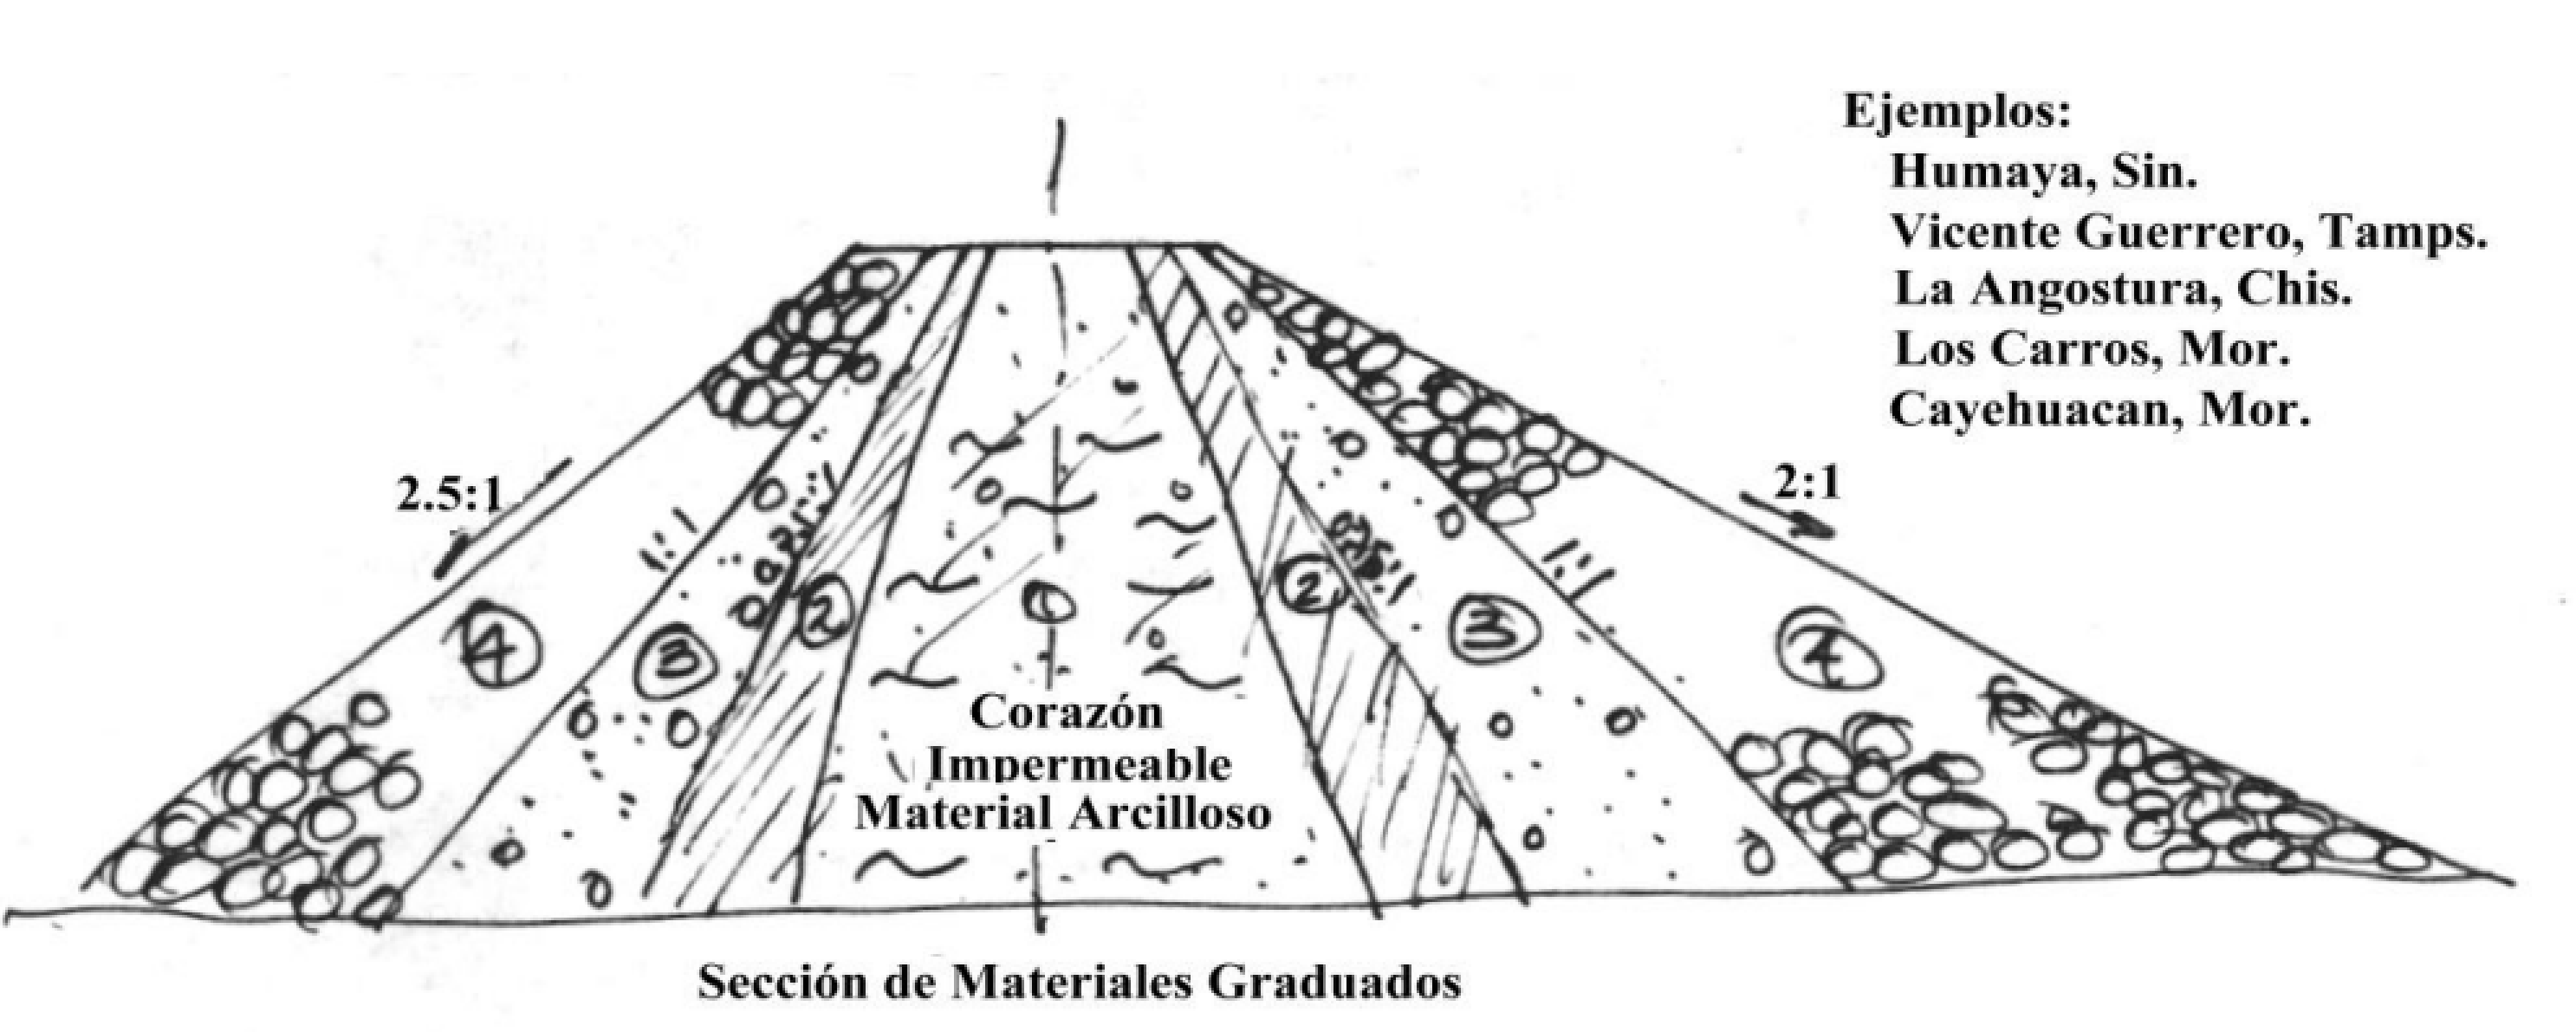
\includegraphics[width=0.5\textwidth]{fii39.png}}
		      \caption{Sección esquemática de presa de tierra tipo materiales graduados.}
		      \label{fii39}
	      \end{figure}
\end{enumerate}

\subsubsection{Presas de enrocamiento}

Estas presas ofrecen características intermedias entre las presas de gravedad y
las presas de tierra.

\begin{enumerate}[noitemsep]
	\item Paramento impermeable
	      \begin{figure}[h!]
		      \centerline{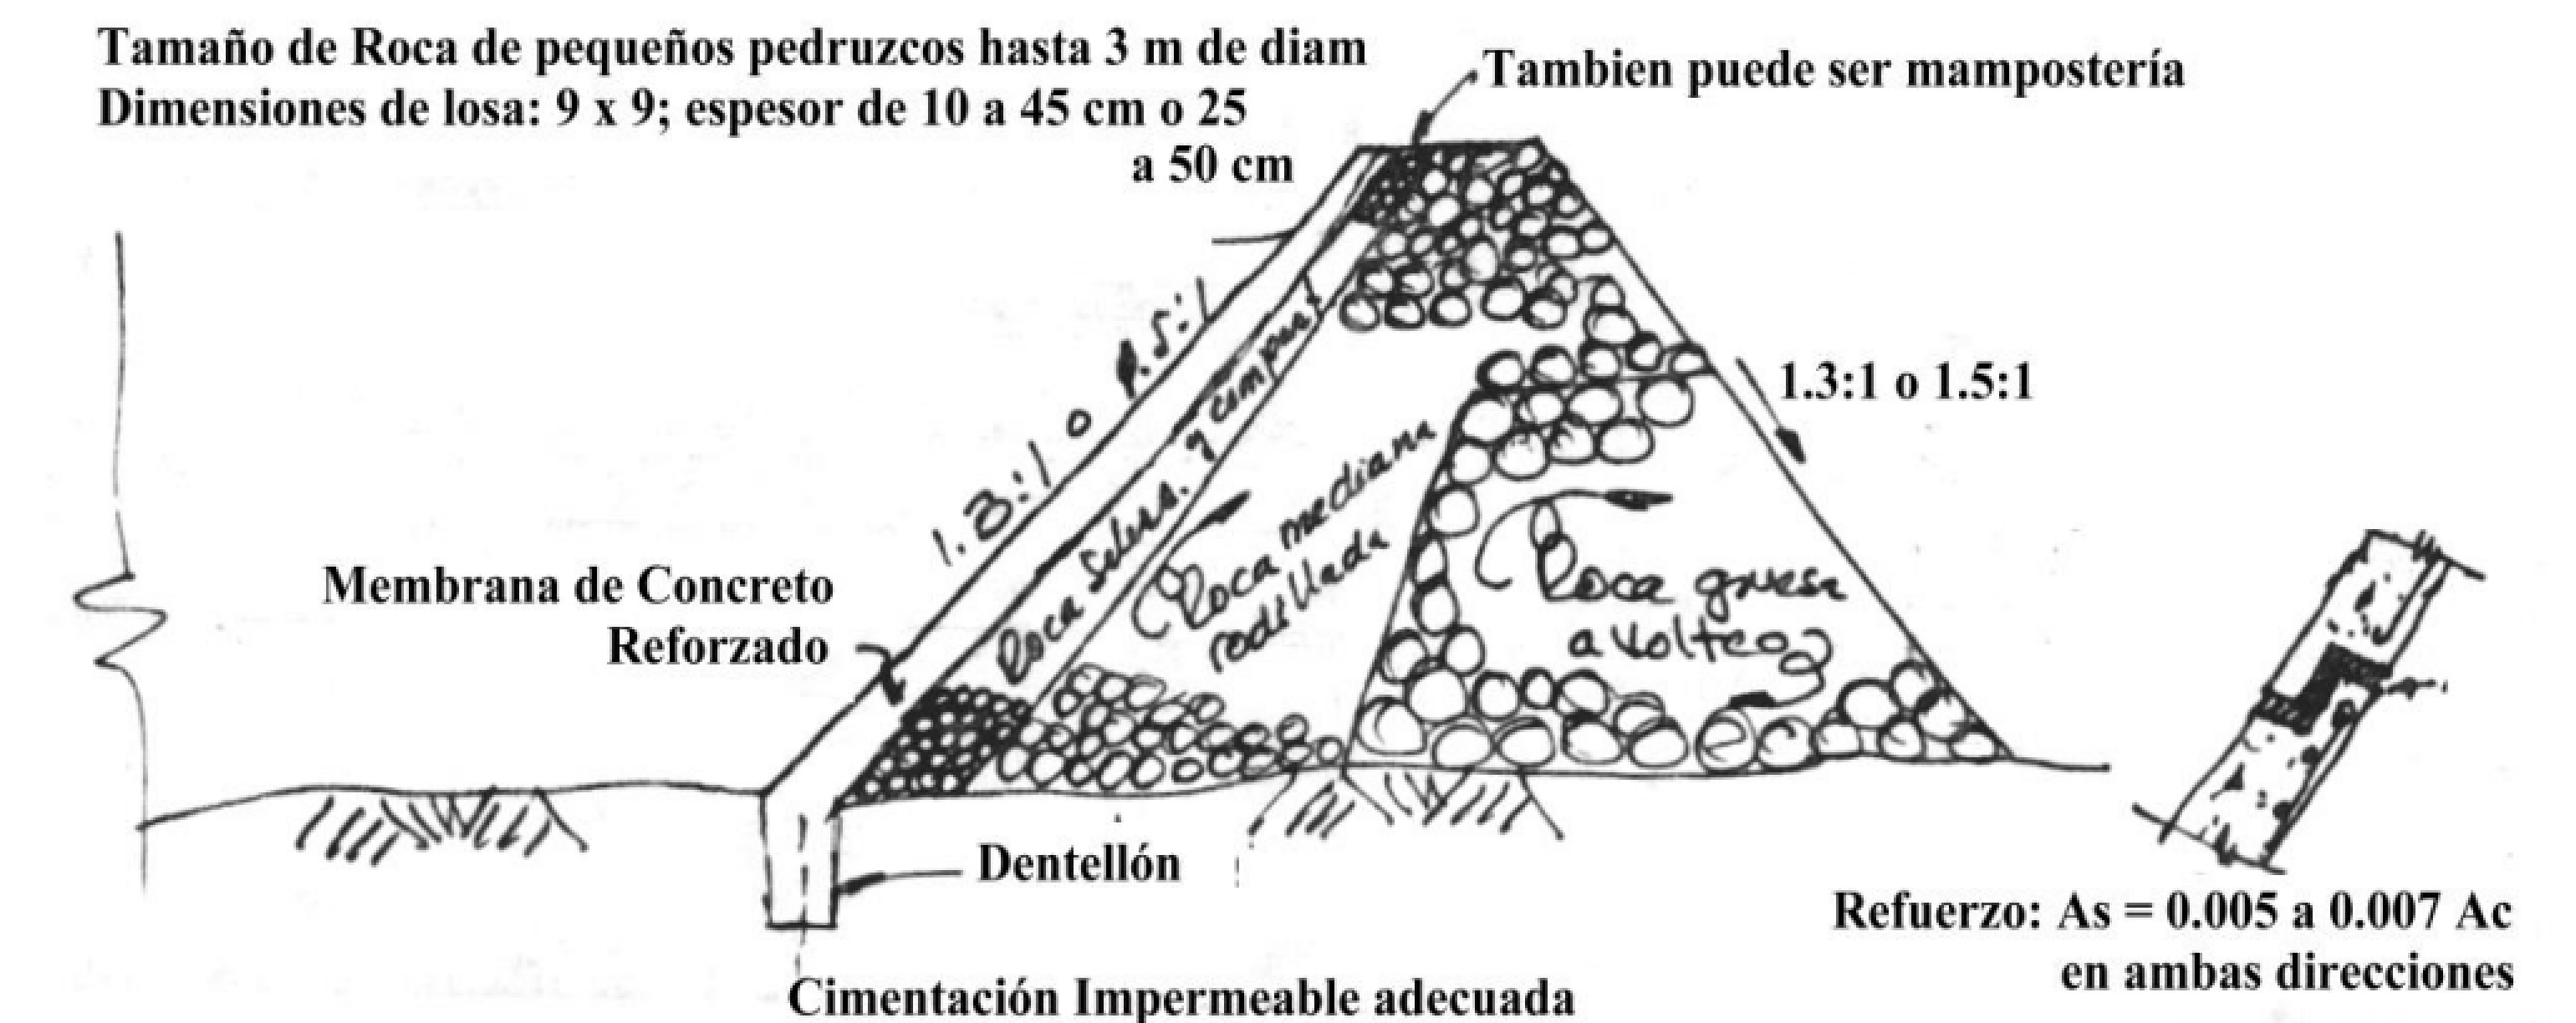
\includegraphics[width=0.5\textwidth]{fii40.png}}
		      \caption{ Sección esquemática de presa de enrocamiento.}
		      \label{fii40}
	      \end{figure}
	      \begin{figure}[h!]
		      \centerline{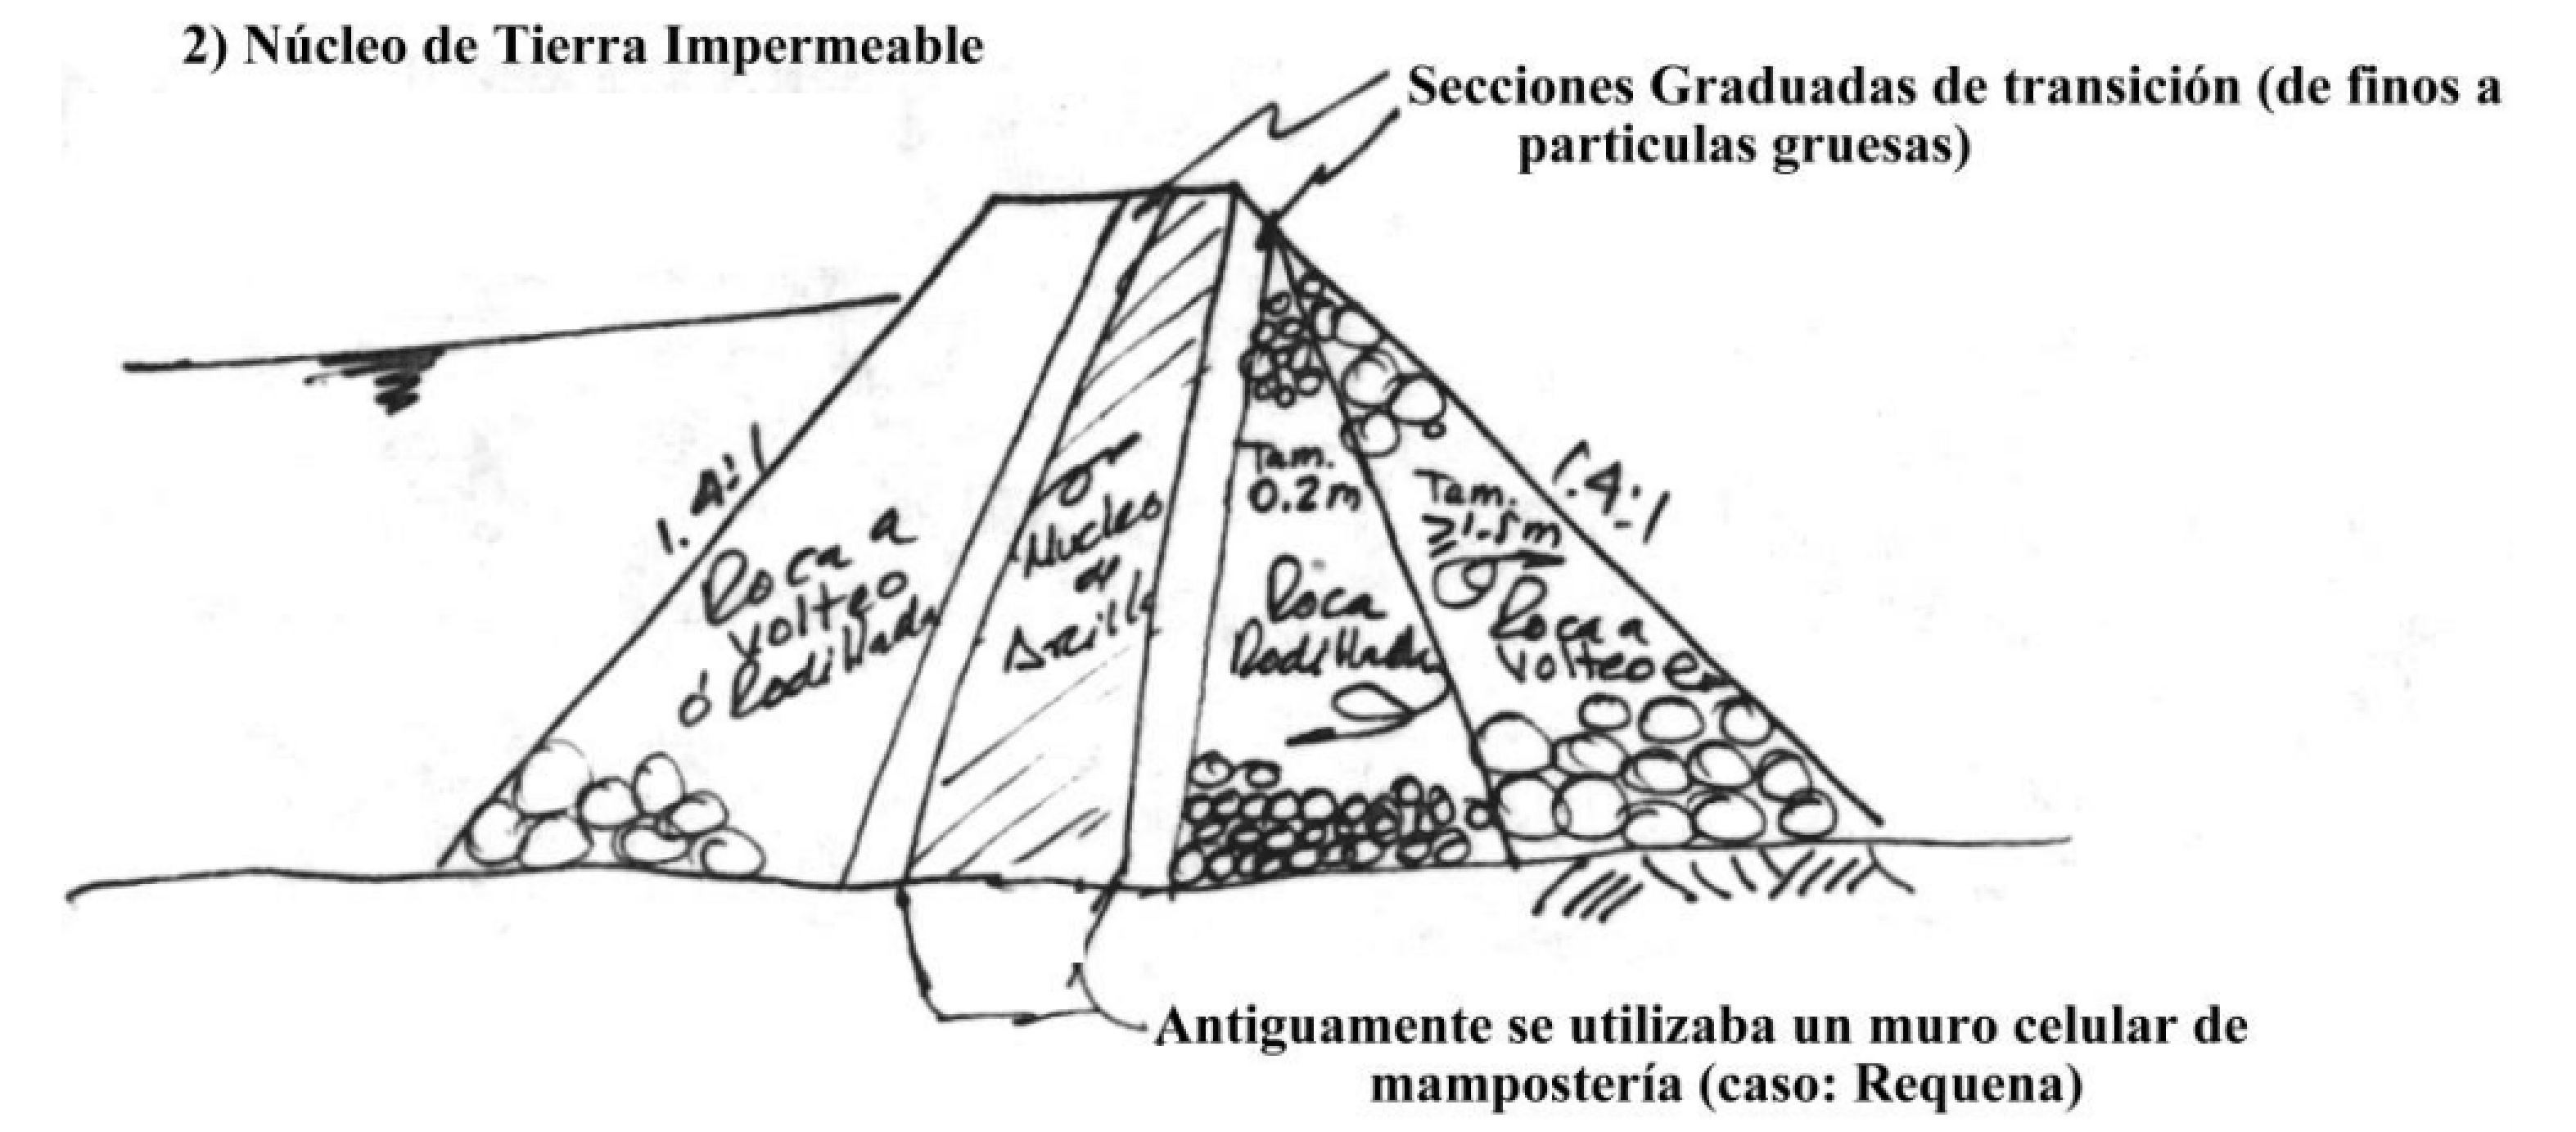
\includegraphics[width=0.5\textwidth]{fii41.png}}
		      \caption{Sección esquemática de presa de enrocamiento con corazón impermeable.}
		      \label{fii41}
	      \end{figure}
	\item Tipos misceláneos de presas: Presas compuestas
	      \begin{figure}[h!]
		      \centerline{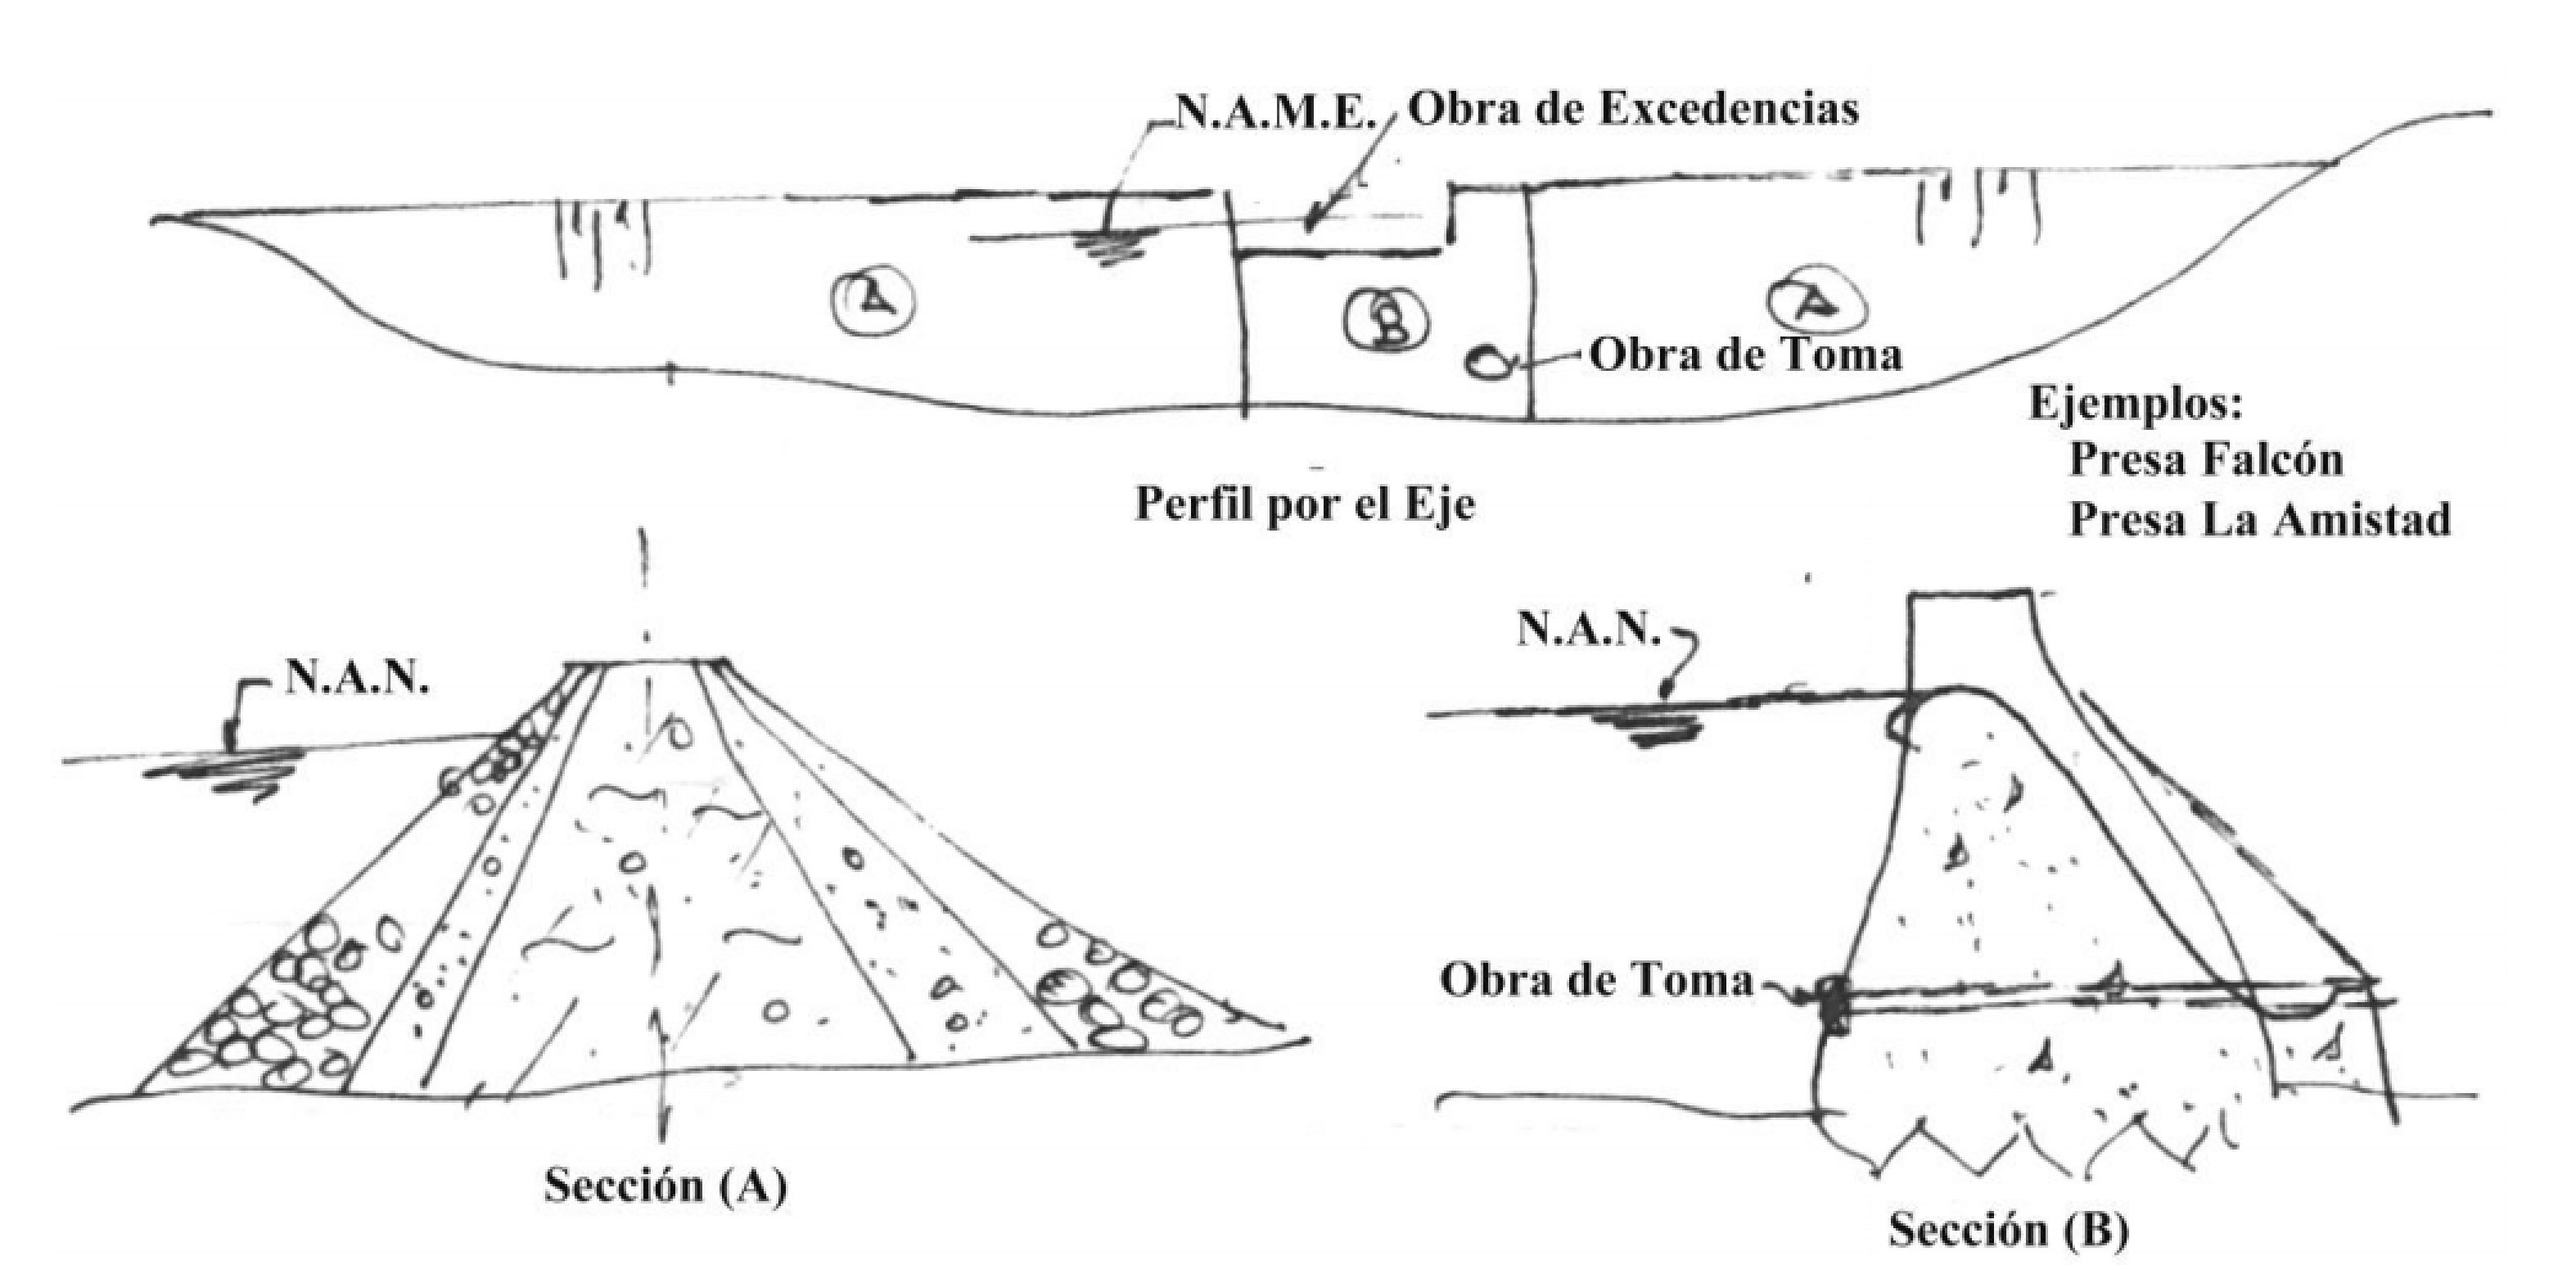
\includegraphics[width=0.5\textwidth]{fii42.png}}
		      \caption{Perfil por el eje y secciones esquemáticas de presa compuesta.}
		      \label{fii42}
	      \end{figure}
\end{enumerate}


\subsection{Obras de desvío}

\begin{definition}[Obras de desvío]
	La obra de desvío es el conjunto de estructuras que tiene por objeto separar o
	desviar el escurrimiento de un río de su cauce natural, durante la etapa de construcción
	de una obra de retención, para poder así trabajar en seco en el sitio de la cortina y
	obras auxiliares. El agua subálvea es aquella que está debajo del álveo de un río o arroyo.
\end{definition}



\subsubsection{Tipo de estructuras integrantes de una obra de desvío.}

Las estructuras integrantes de una obra de desvío pueden ser:
\begin{enumerate}[noitemsep]
	\item  Canal o Tajo temporal
	      \begin{figure}[h!]
		      \centerline{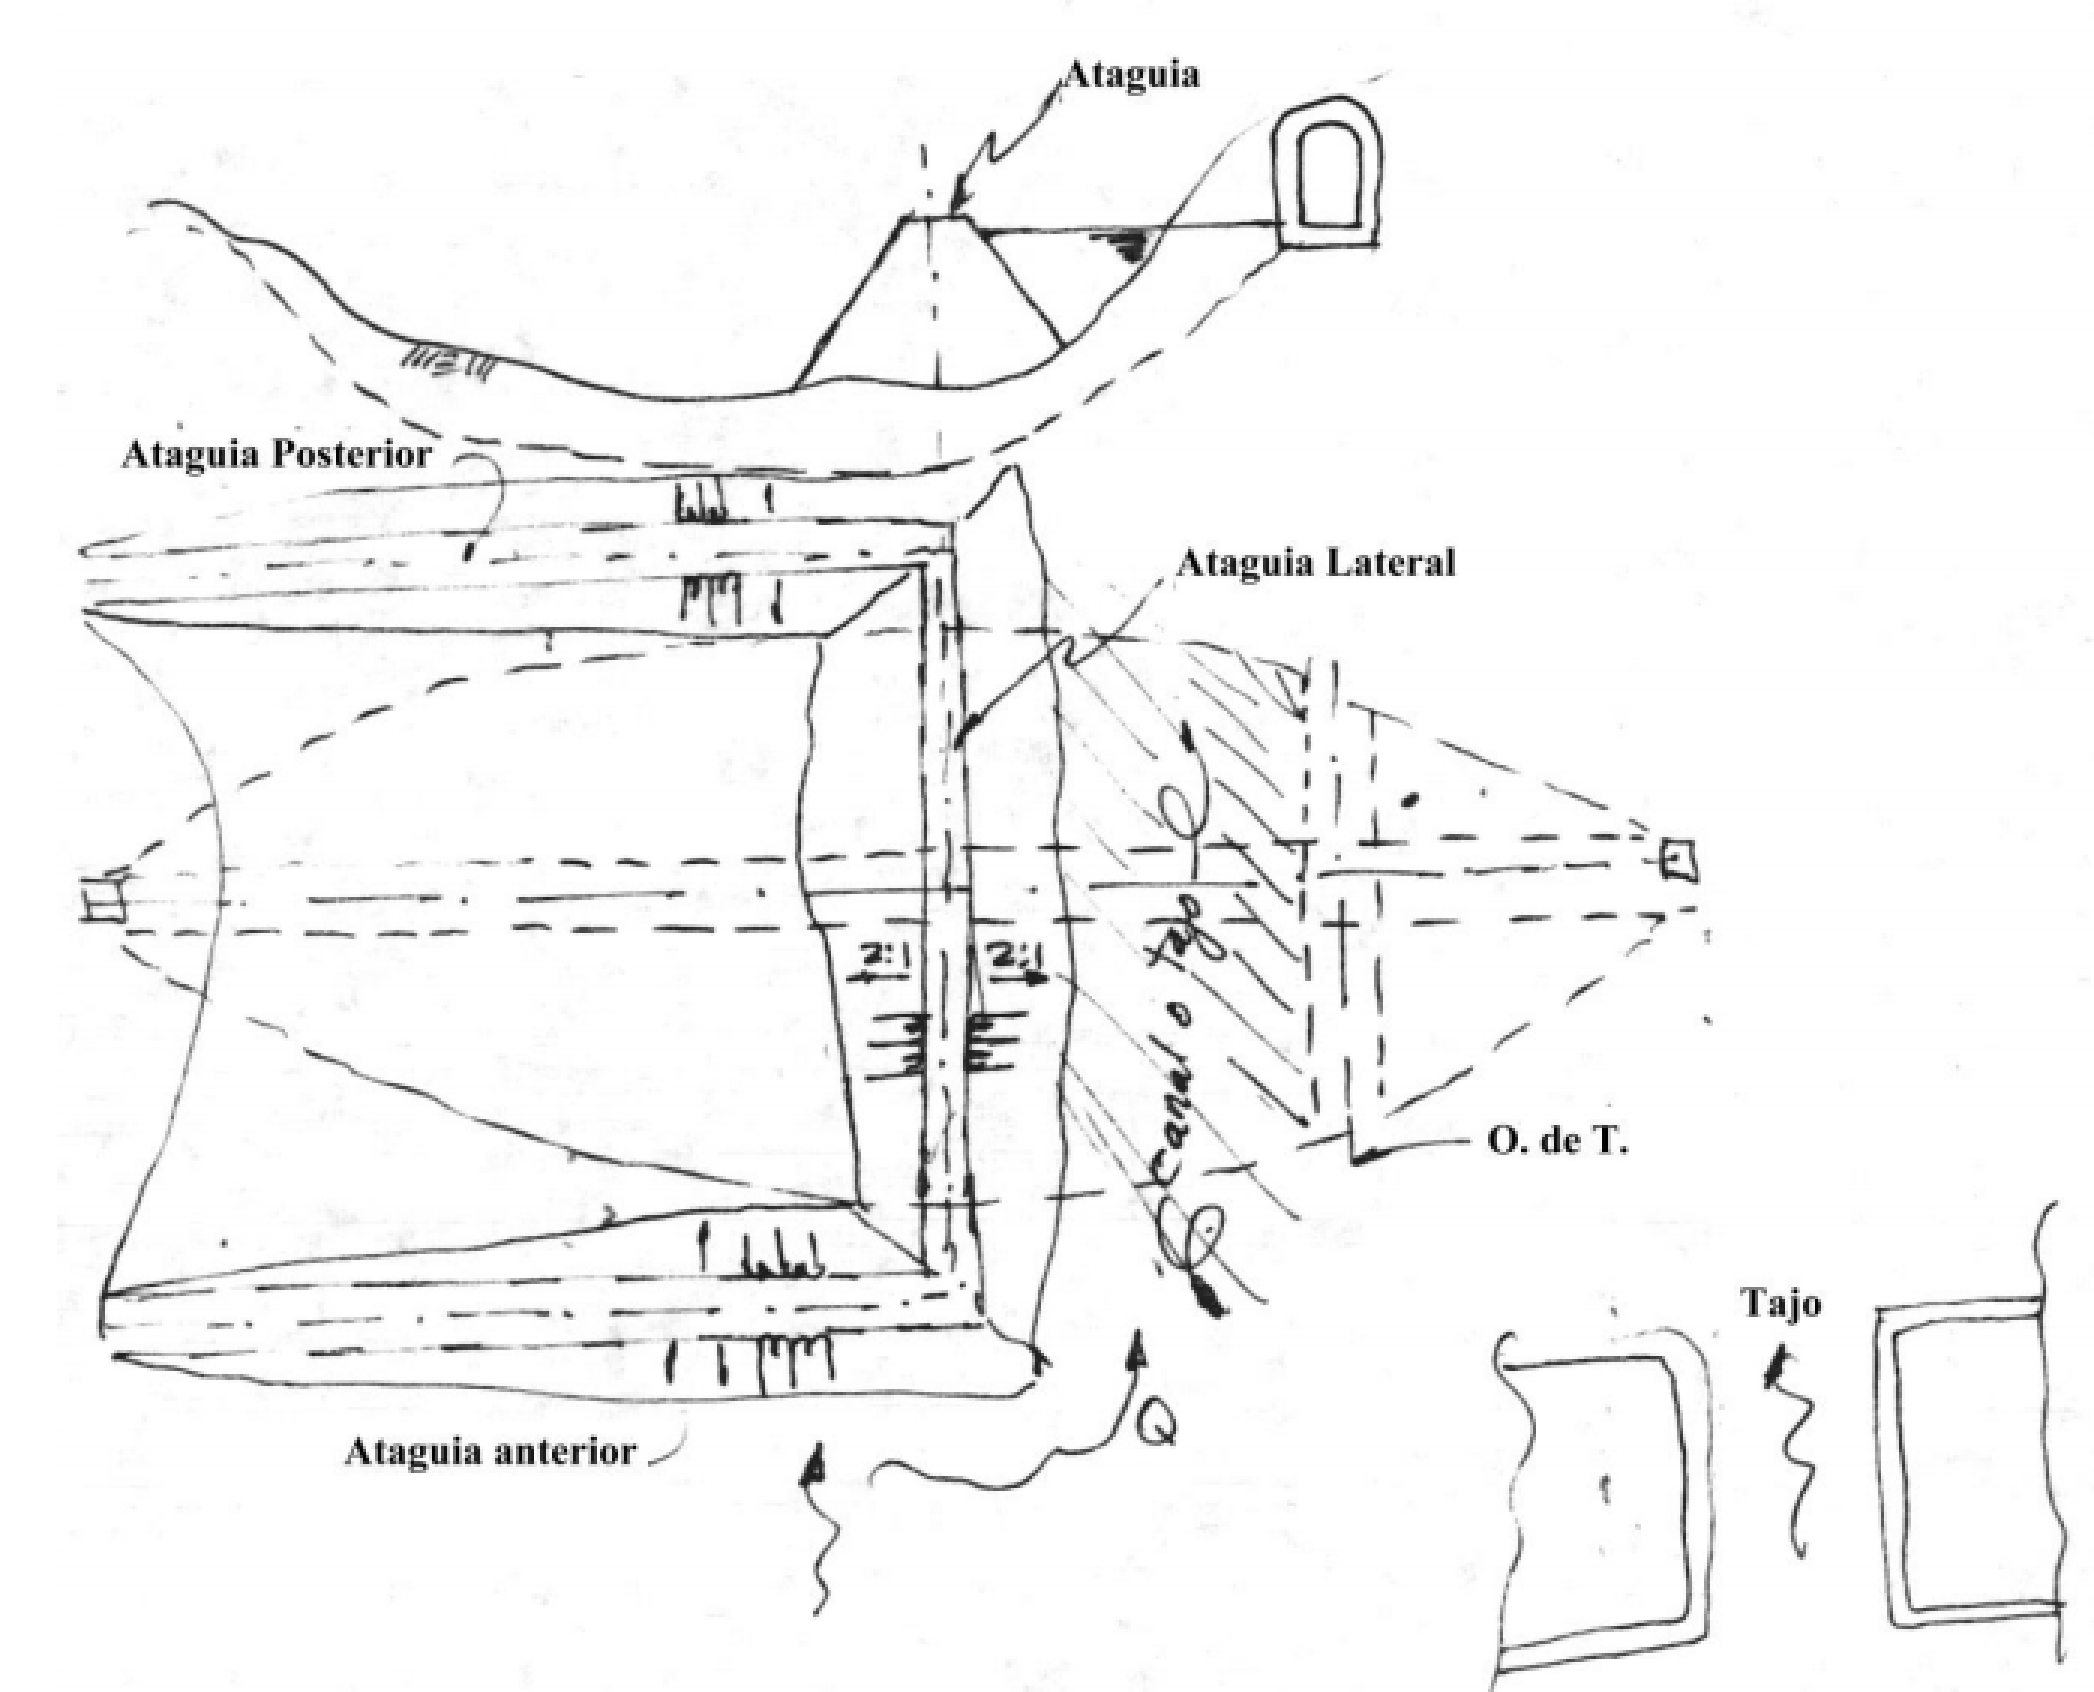
\includegraphics[width=0.5\textwidth]{fii43.png}}
		      \caption{Obra de desvío conformada con un canal o tajo temporal.}
		      \label{fii43}
	      \end{figure}
	\item  Hueco o paso temporal a través de la cortina de concreto
	\item  Conducto a través del cuerpo de una cortina de materiales graduados
	\item  Túneles a través de las laderas de las boquillas
\end{enumerate}

La Ataguía es un dique o barrera temporal que se emplea para desviar la
corriente o para encerrar un área determinada, permitiendo la construcción dentro de
ella, aún por debajo del nivel del escurrimiento.

\begin{enumerate}
	\item Tierra
	\item Tabla estacados:Madera o acero hincados en el terreno y apoyados por una serie de
	      marcos de madera o fierro para resistir el empuje. Ó Enhuacalados de madera, relleno de roca con tierra
	      \begin{figure}[h!]
		      \centerline{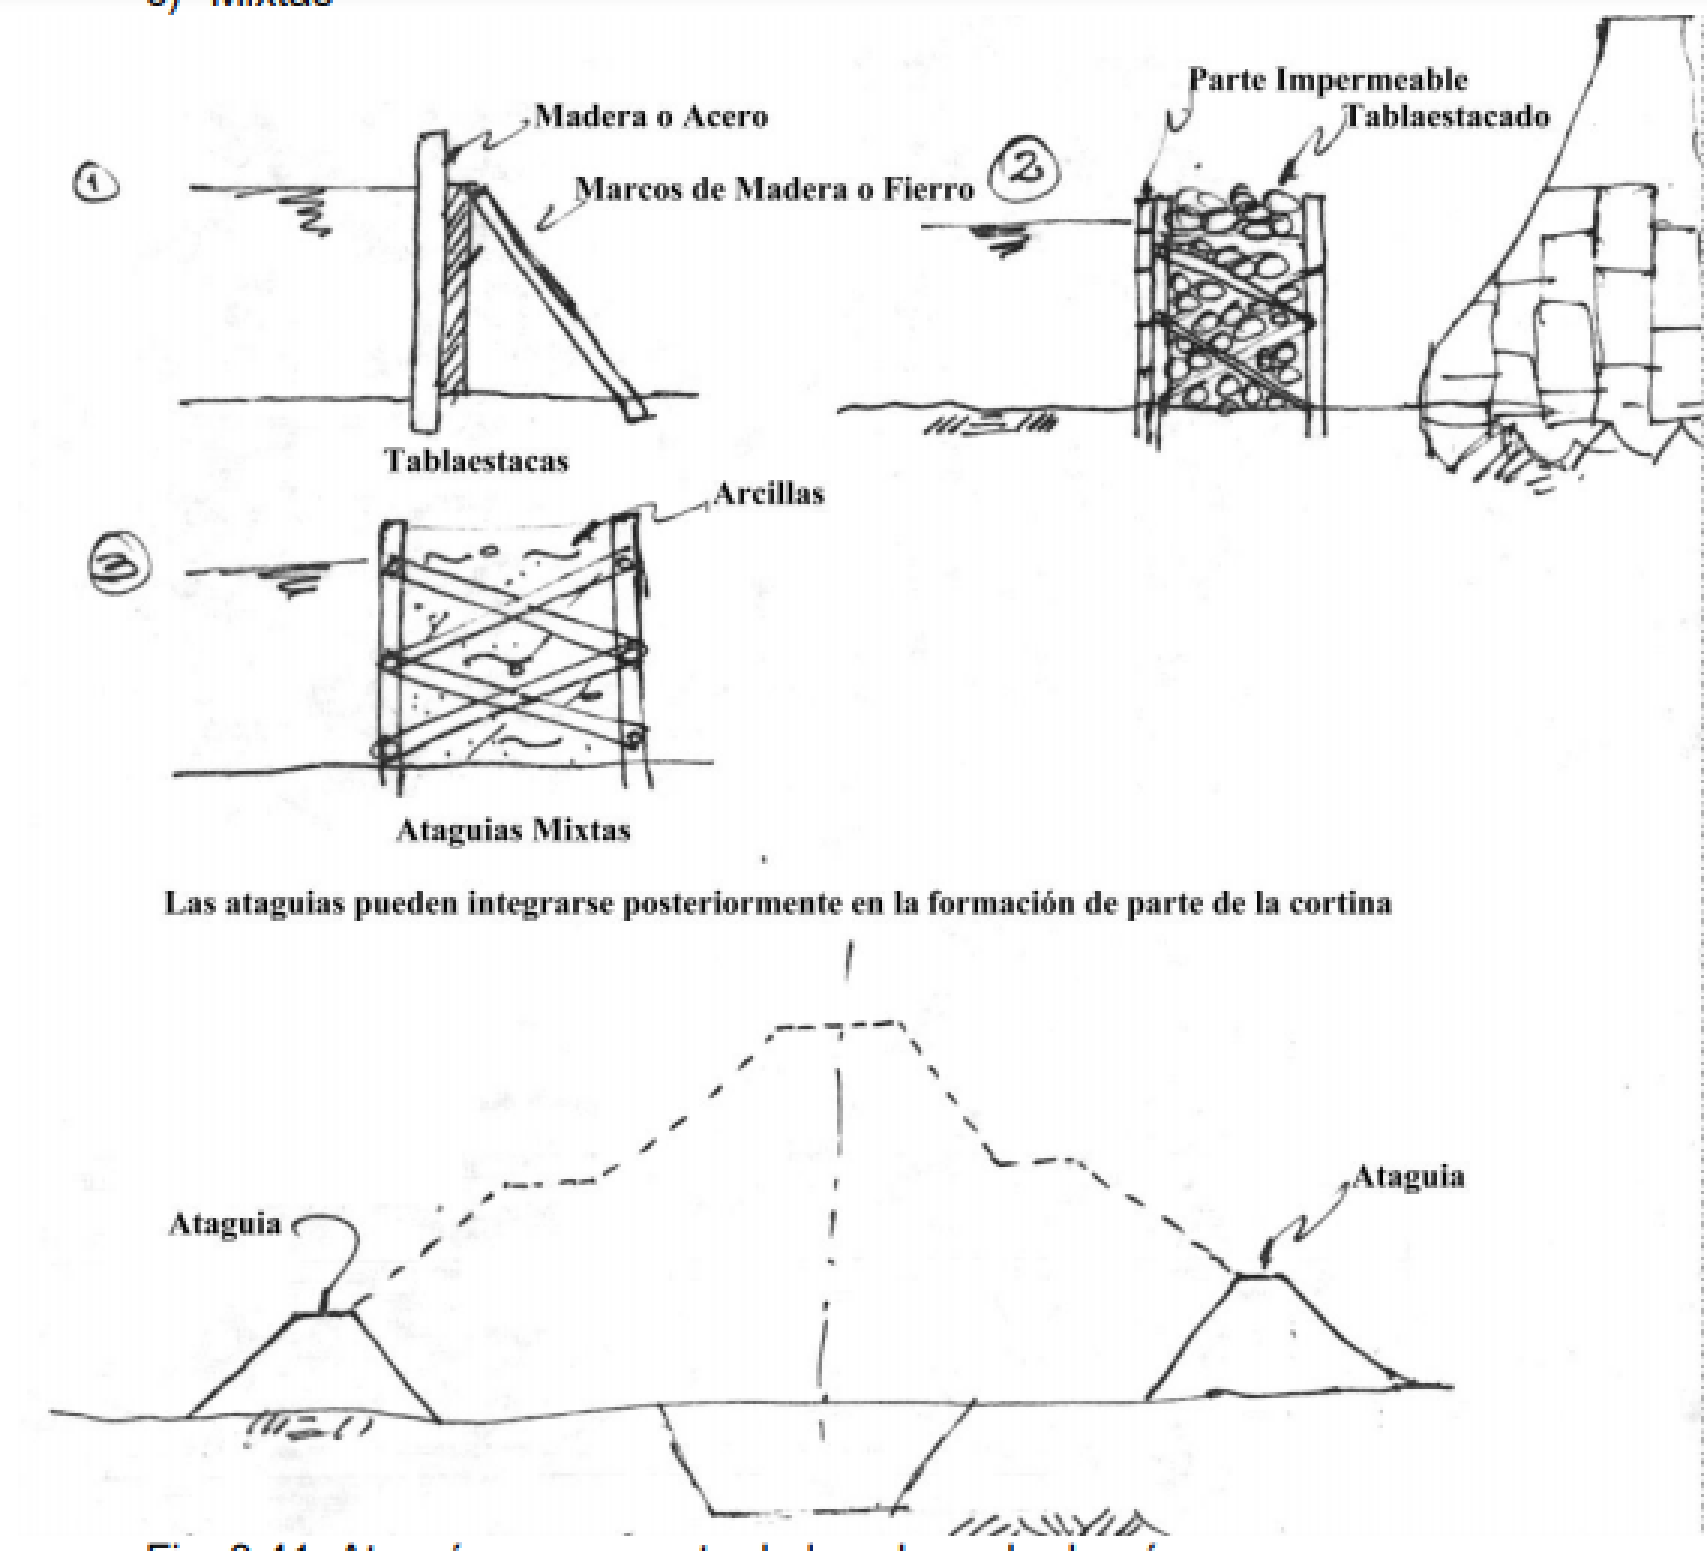
\includegraphics[width=0.5\textwidth]{fii44.png}}
		      \caption{Ataguías como parte de las obras de desvío.}
		      \label{fii44}
	      \end{figure}
	\item Mixtas
\end{enumerate}

Las principales consideraciones para la planeación de las ataguías son:

\begin{enumerate}
	\item Suficiente altura
	\item Seguridad durante el periodo de desvío
	\item Previsión para removerlas cuando ya no se empleen.
\end{enumerate}

\textbf{Hueco o paso temporal} a través de la cortina de concreto
Características: Son muy caros, pero más efectivos, mantienen seco el lugar de construcción, trabajan a superficie libre
Pueden ir revestidos, reforzados con acero y concreto, o ademado con  acero. Forman parte de la obra de toma u obra de excedencias (infiernillo). Son para obras de gran importancia.

\begin{figure}[h!]
	\centerline{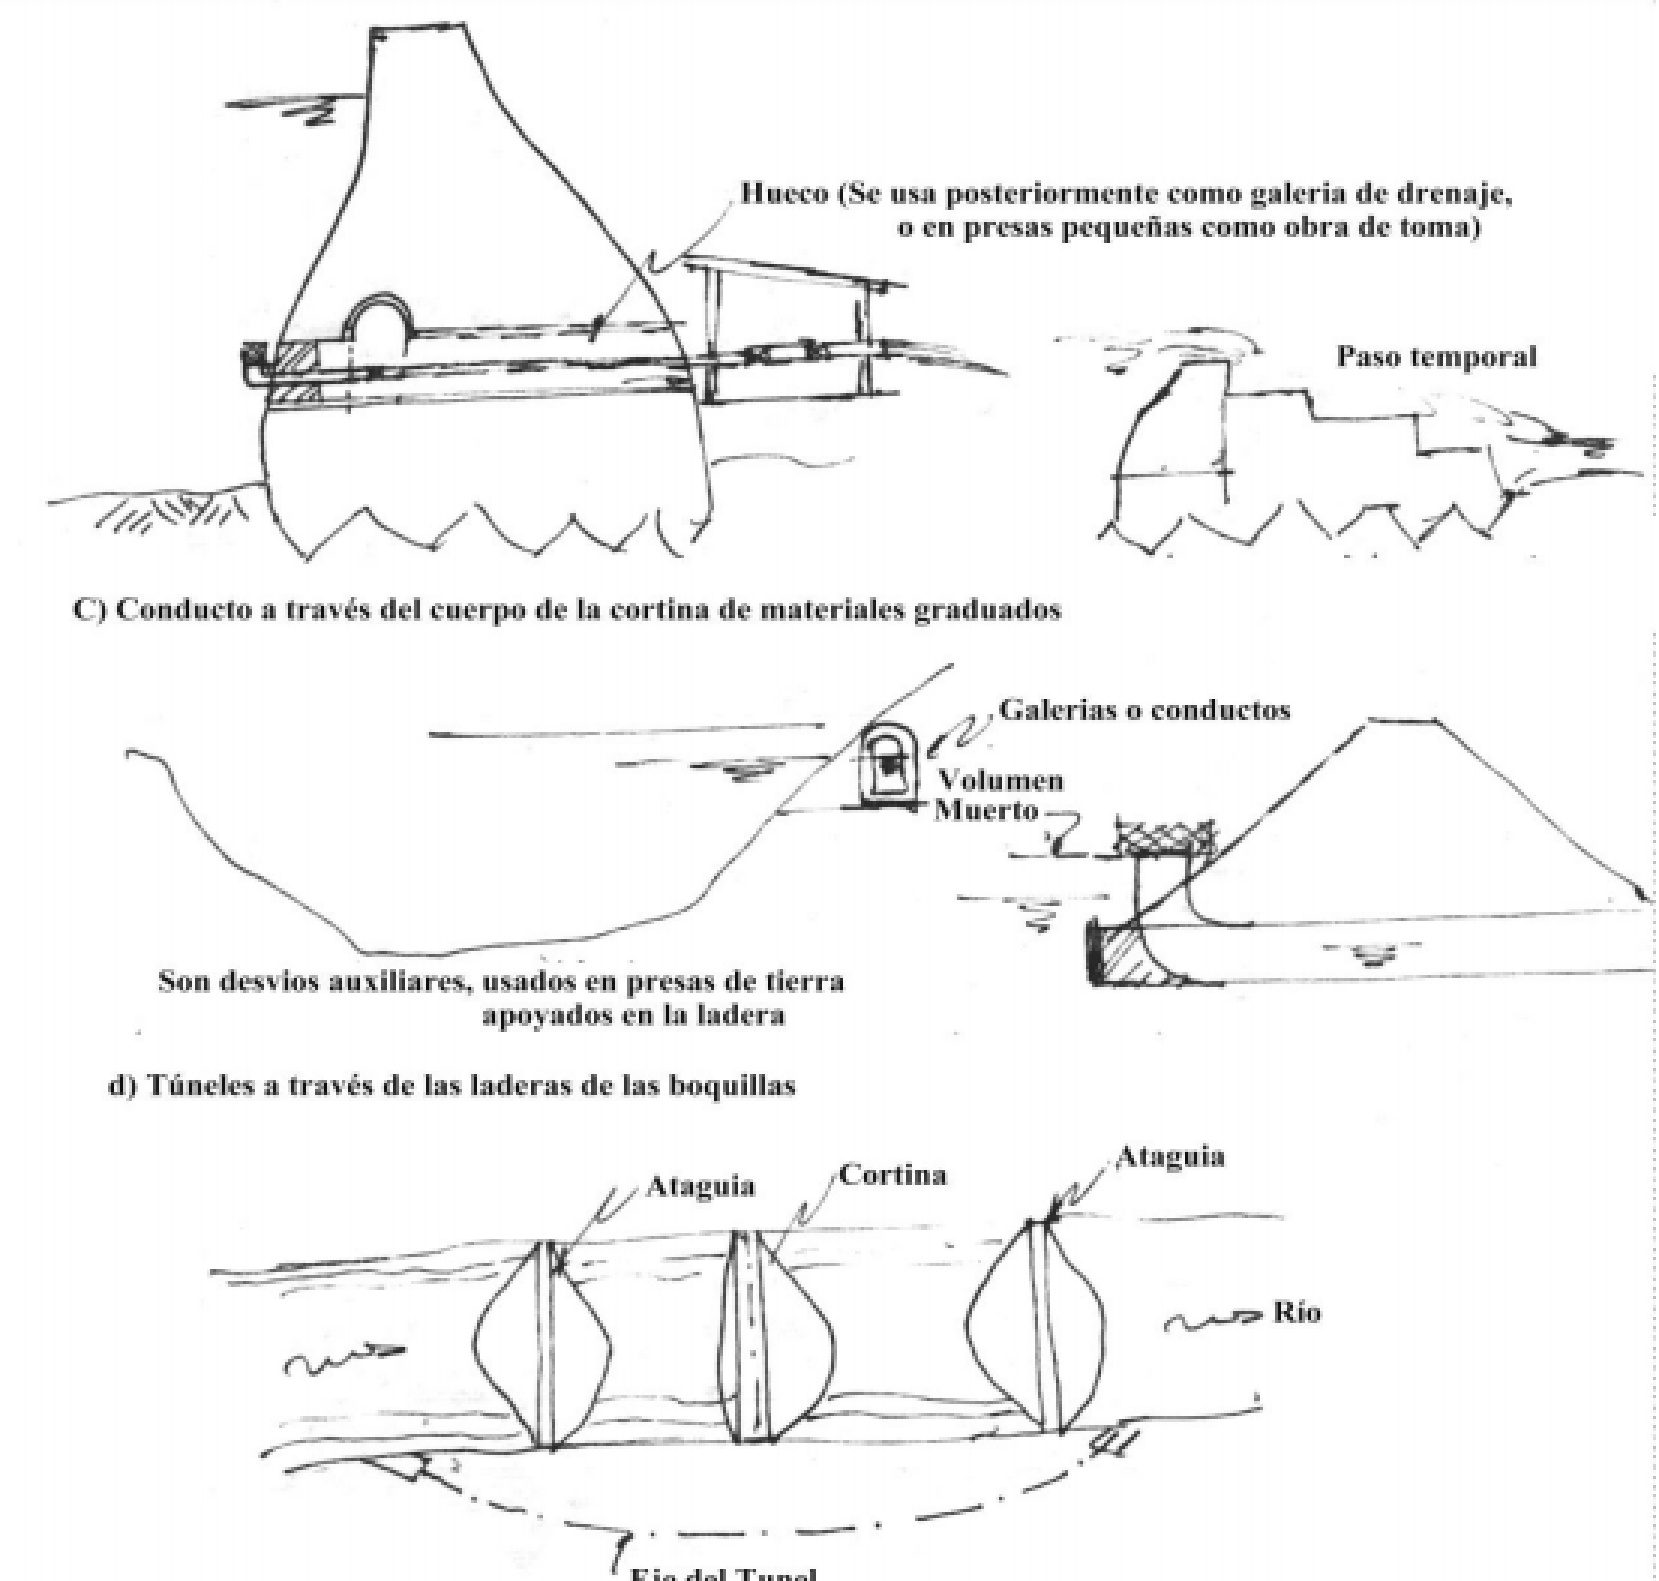
\includegraphics[width=0.5\textwidth]{fii45.png}}
	\caption{Obras de desvío bajo diferentes alternativas.}
	\label{fii45}
\end{figure}



\subsubsection{Obras de Toma:} La función de esta obra es manejar las extracciones para
satisfacer la demanda que los diferentes beneficios exigen.


\subsubsection{Obras de excedencias:} La función es dar salida a las aguas de escurrimiento que
no pueden ser almacenadas por haber llegado a un cierto nivel que muestra la
capacidad total.



\subsection{Obras de toma}

\begin{definition}[Obras de toma]
	La obra de toma es el conjunto de estructuras y equipos requeridos para la
	operación segura y controlada del agua embalsada, extraída con el objeto de satisfacer
	las necesidades de las demandas, para el cual fue proyectado el almacenamiento.
\end{definition}

\subsubsection{Partes esenciales}

\begin{itemize}
	\item Conductos (canal, tubería, túnel y/o galería)
	\item Sistemas de obturación (estructura mecánica con elementos de cierre).
\end{itemize}

Ordenamiento de las partes en el sentido de la corriente:

\begin{enumerate}
	\item Canal de acceso
	\item Estructura de rejillas
	\item Conducto
	\item Equipo y sistema de obturación
	\item Elementos de protección y control
	\item Estructuras terminales
\end{enumerate}

\subsubsection{Clasificación de las obras de toma}

\begin{enumerate}[noitemsep]
	\item Según el propósito
	      \begin{enumerate}
		      \item Para generar energía
		      \item Para riego
		      \item Para finalidades múltiples
	      \end{enumerate}
	\item Según la ubicación del sistema de operación
	      \begin{enumerate}
		      \item Que se opera en la entrada de la obra de toma o del conducto
		      \item Que se opera en la parte media del conducto
		      \item Que se opera al final del conducto
	      \end{enumerate}
	\item Según la estructura donde se ubica el mecanismo de obturación
	      \begin{enumerate}
		      \item Tipo Torre
		      \item Tipo lumbrera
		      \item Tipo tubería a presión y válvulas
	      \end{enumerate}
	\item Según el tipo de construcción del conducto
	      \begin{enumerate}
		      \item Conducto excavado y colado a cielo abierto
		      \item Túneles perforados en las laderas
		      \item Conducto ahogado en el cuerpo de la cortina
	      \end{enumerate}
	\item Según la posición de la Obra de Toma
	      \begin{enumerate}
		      \item En una de las márgenes
		      \item En ambas márgenes
		      \item En un solo nivel
		      \item En varios niveles (Toma alta, toma baja)
	      \end{enumerate}
	\item Según la característica de la descarga.
	      \begin{enumerate}
		      \item Se descarga a un canal de conducción
		      \item Se descarga directamente al río
		      \item Descarga a un sistema de tubería forzada (a presión)
	      \end{enumerate}
\end{enumerate}

\subsubsection{Localización de la Obra de Toma}

\begin{enumerate}
	\item Respecto a la cortina.
	      \begin{enumerate}
		      \item En el cuerpo de la cortina (sólo de materiales rígidos: gravedad (de concreto
		            o mampostería, arco, arco-gravedad, etc$\dots$)
		      \item Fuera del cuerpo de la cortina (utilizada en cortinas de materiales flexibles,
		            ubicada en una de las laderas en excavación o en perforación de túnel).
	      \end{enumerate}
	\item Respecto a niveles de almacenamiento
\end{enumerate}

El nivel de la obra de toma, lo fija el N.A.mín. (Nivel de Aguas mínimo) dado por
la capacidad muerta en el almacenamiento, integrado por el volumen de azolves, cría
de peces, recreación y otros.

\subsubsection{Tipos más frecuentes de Obra de Toma}

\begin{enumerate}[noitemsep]
	\item Canal en tomas Altas
	\item Torre y galería (funcionando como canal)
	      \begin{figure}[h!]
		      \centerline{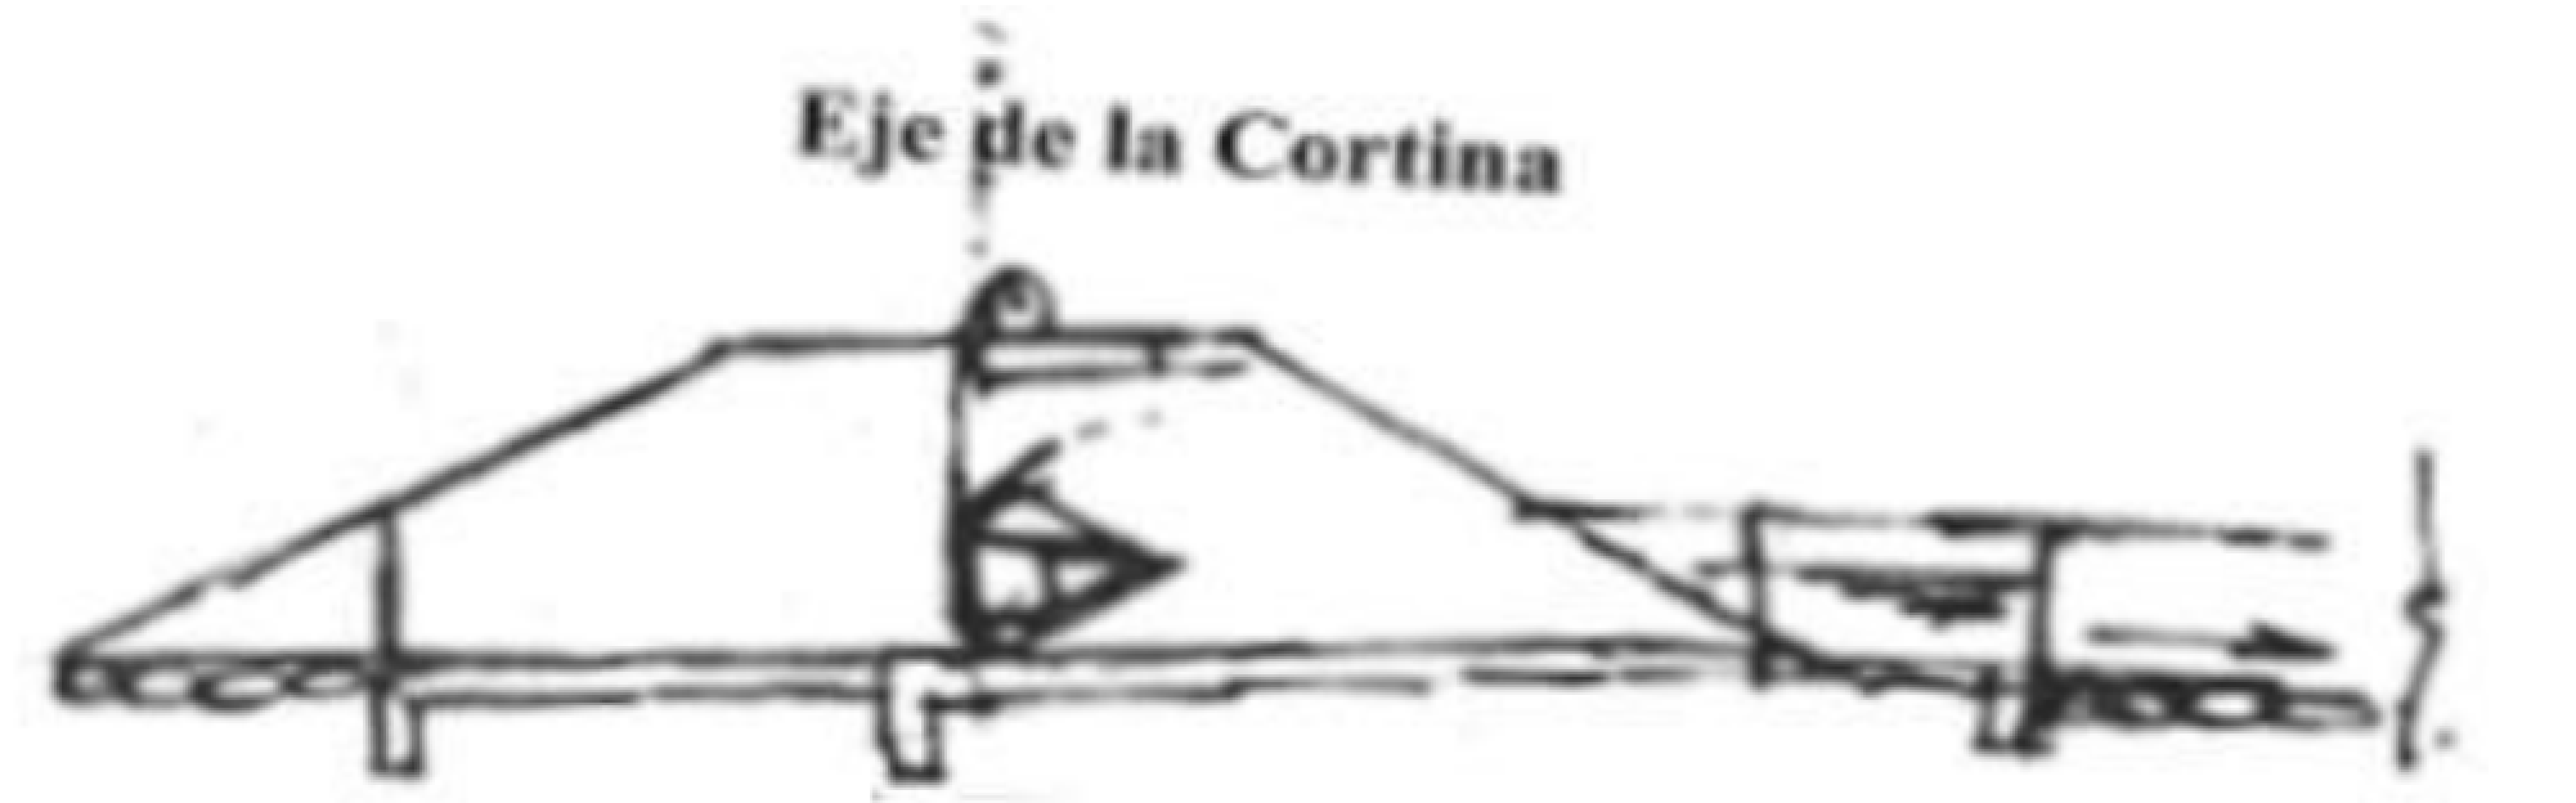
\includegraphics[width=0.5\textwidth]{fii46.png}}
		      \caption{Perfil esquemático de obra de toma tipo torre y galería.}
		      \label{fii46}
	      \end{figure}
	\item Tubería a presión
	      \begin{figure}[h!]
		      \centerline{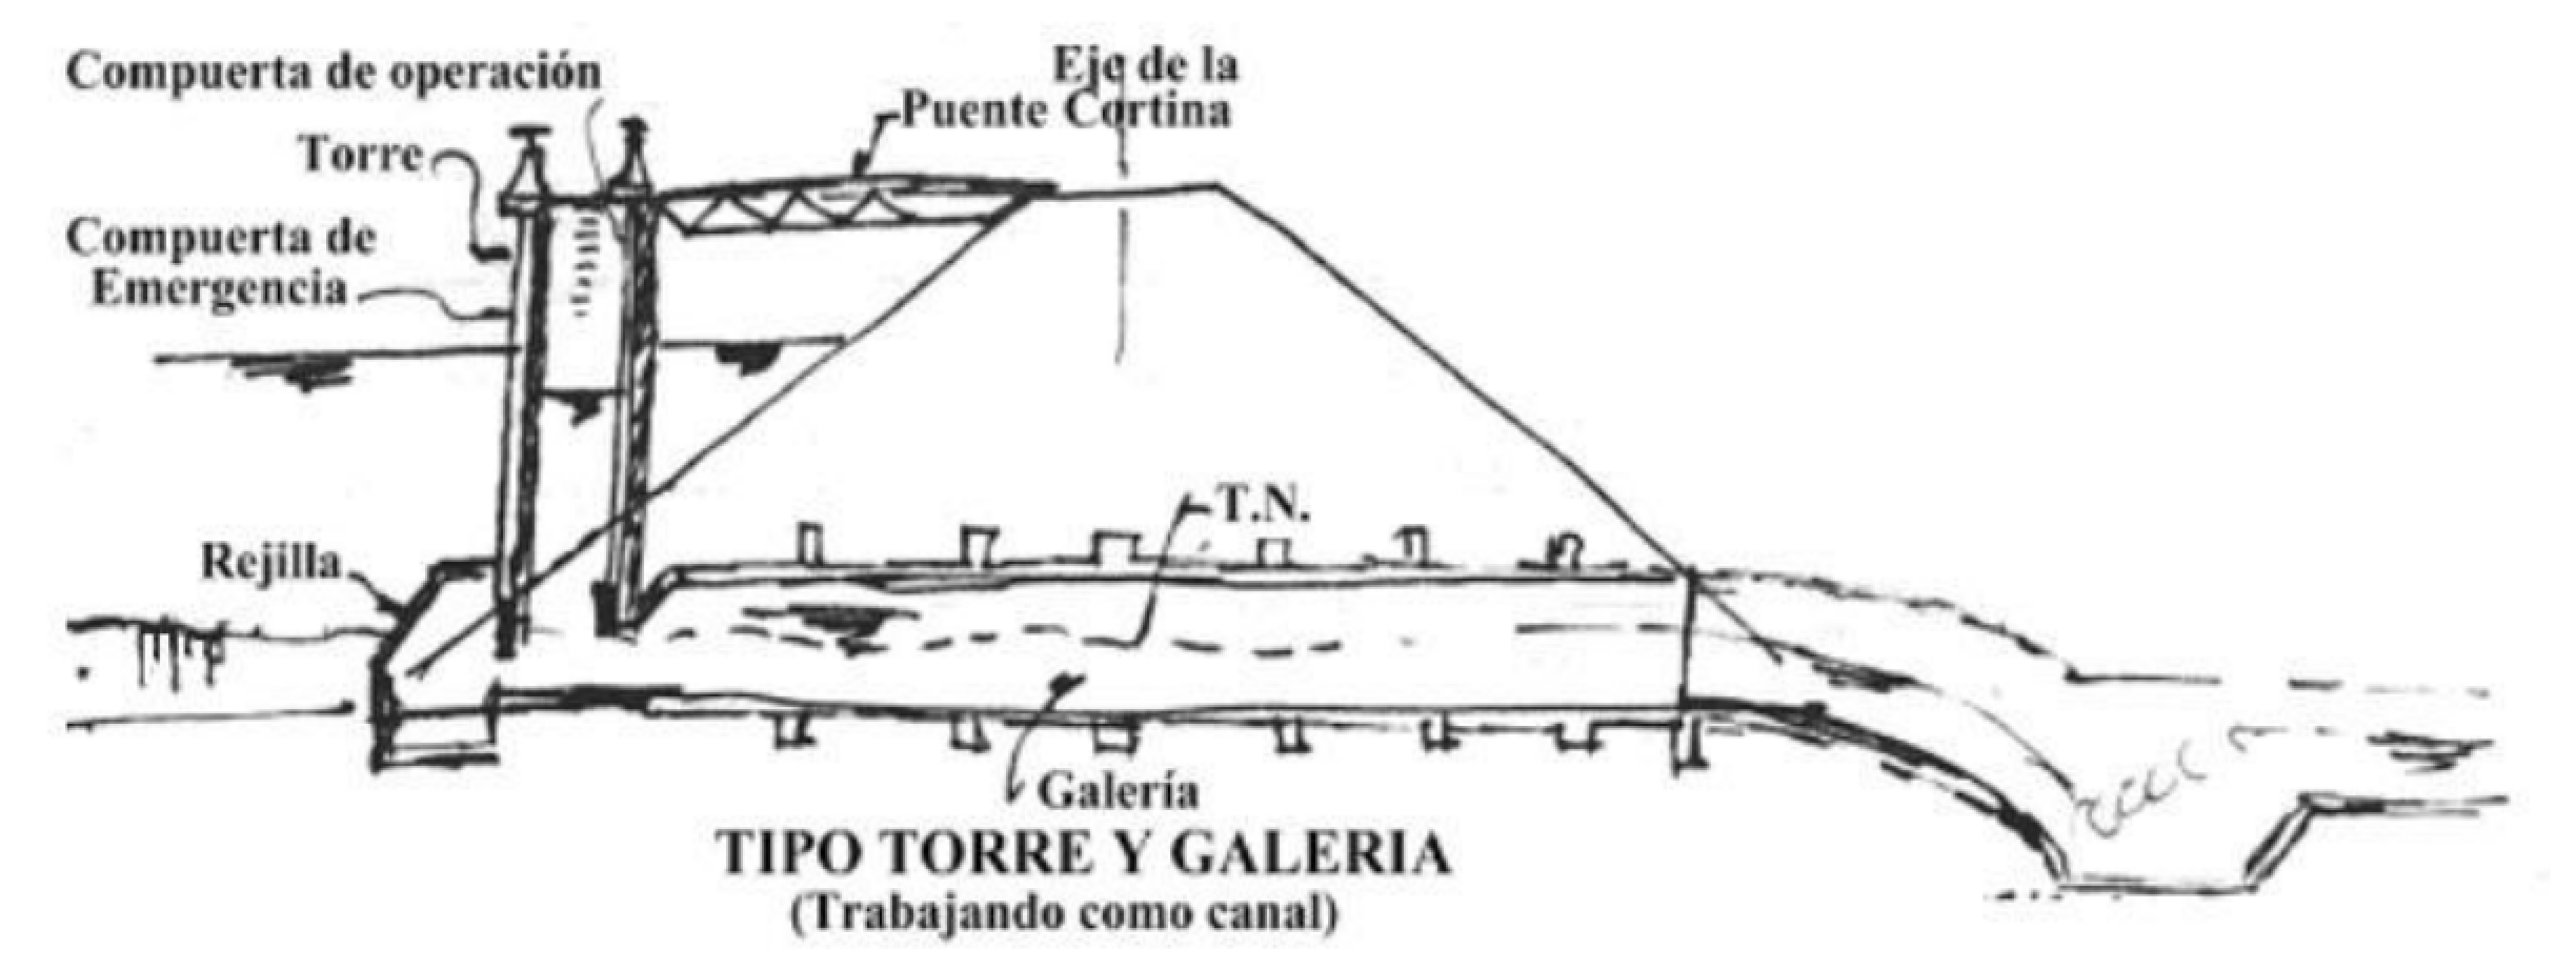
\includegraphics[width=0.5\textwidth]{fii47.png}}
		      \caption{Perfil esquemático de obra de toma tipo tubería a presión y válvulas a
			      la salida.}
	      \end{figure}
	      \label{fii47}
	\item Galería con tubería a presión
	      \begin{figure}[h!]
		      \centerline{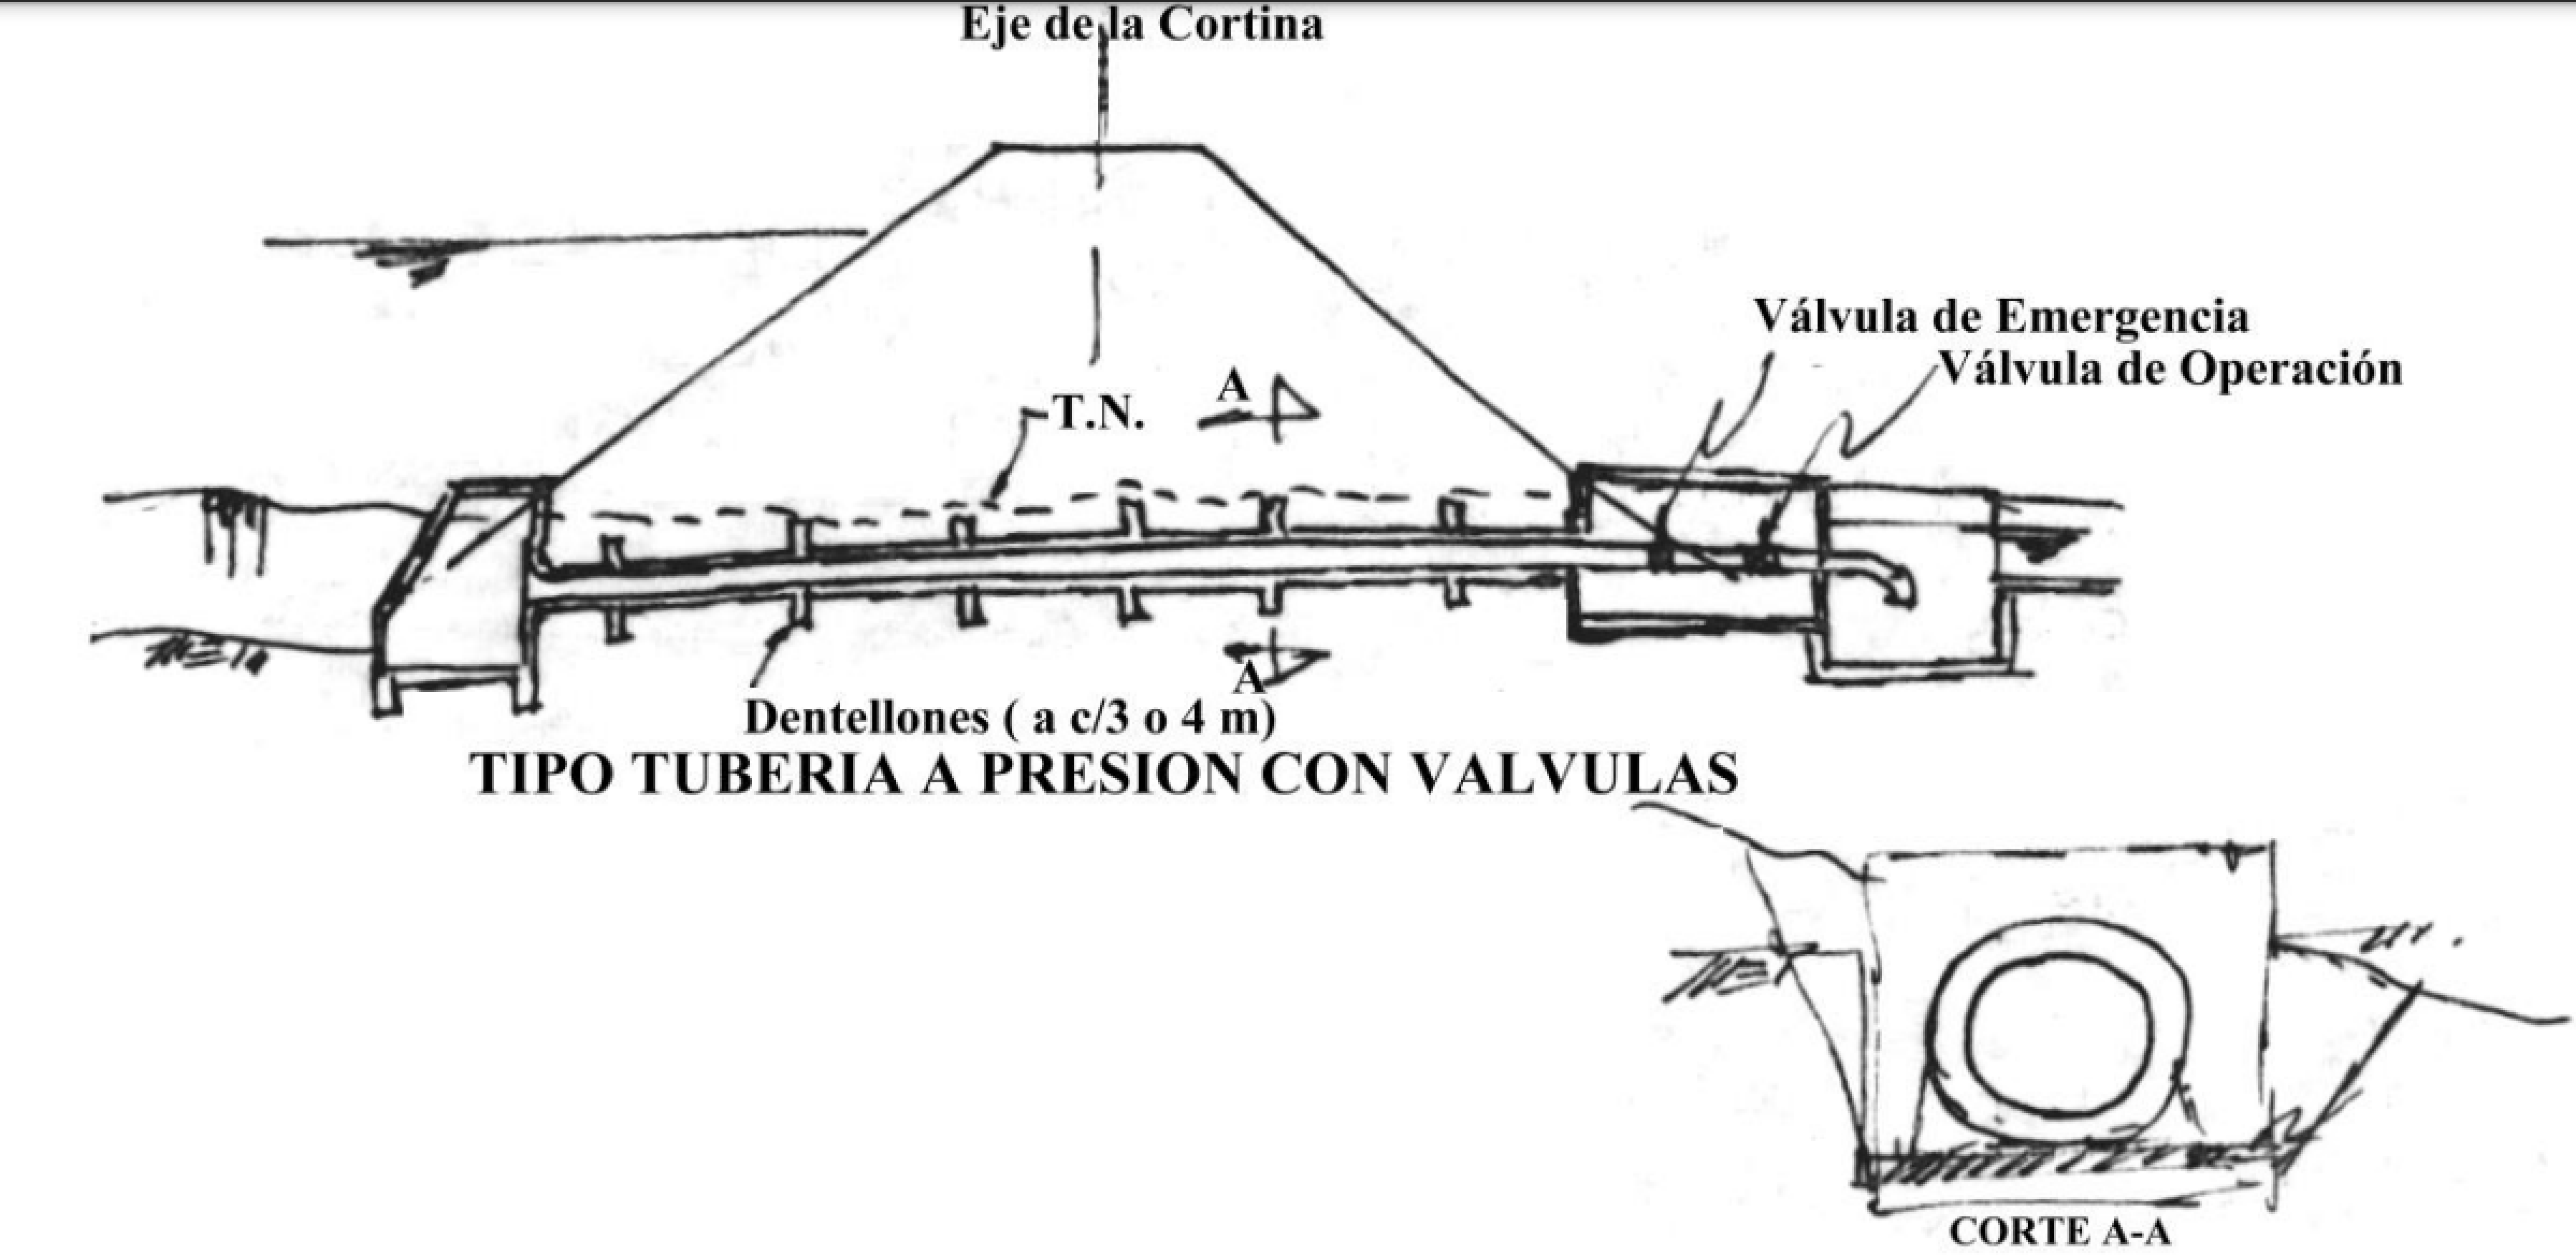
\includegraphics[width=0.5\textwidth]{fii48.png}}
		      \caption{Perfil esquemático de obra de toma tipo tubería a presión y válvulas a
			      la salida.}
		      \label{fii48}
	      \end{figure}
	\item Tipos mixtos.
\end{enumerate}

\subsection{Obras de excedencias}

\begin{definition}[Obras de excedencias]
	La obra de excedencias o vertedor de demasías es la estructura que tiene por
	objeto dar salida a las aguas excedentes del almacenamiento, protegiendo la cortina,
	obra de toma y demás estructuras al impedir que el agua, que ya no puede ser
	almacenada (por rebasar el N.A.N.), desborde sobre la obra de retención y la destruya.
\end{definition}

\subsubsection{Partes de que consta}

\begin{itemize}
	\item Canal de acceso
	\item Cresta vertedora
	\item Canal colector
	\item Sección de control
	\item Canal de descarga
	\item Estructura disipadora o disipador de energía
	\item Canal de salida al cauce
\end{itemize}

\begin{figure}[h!]
	\centerline{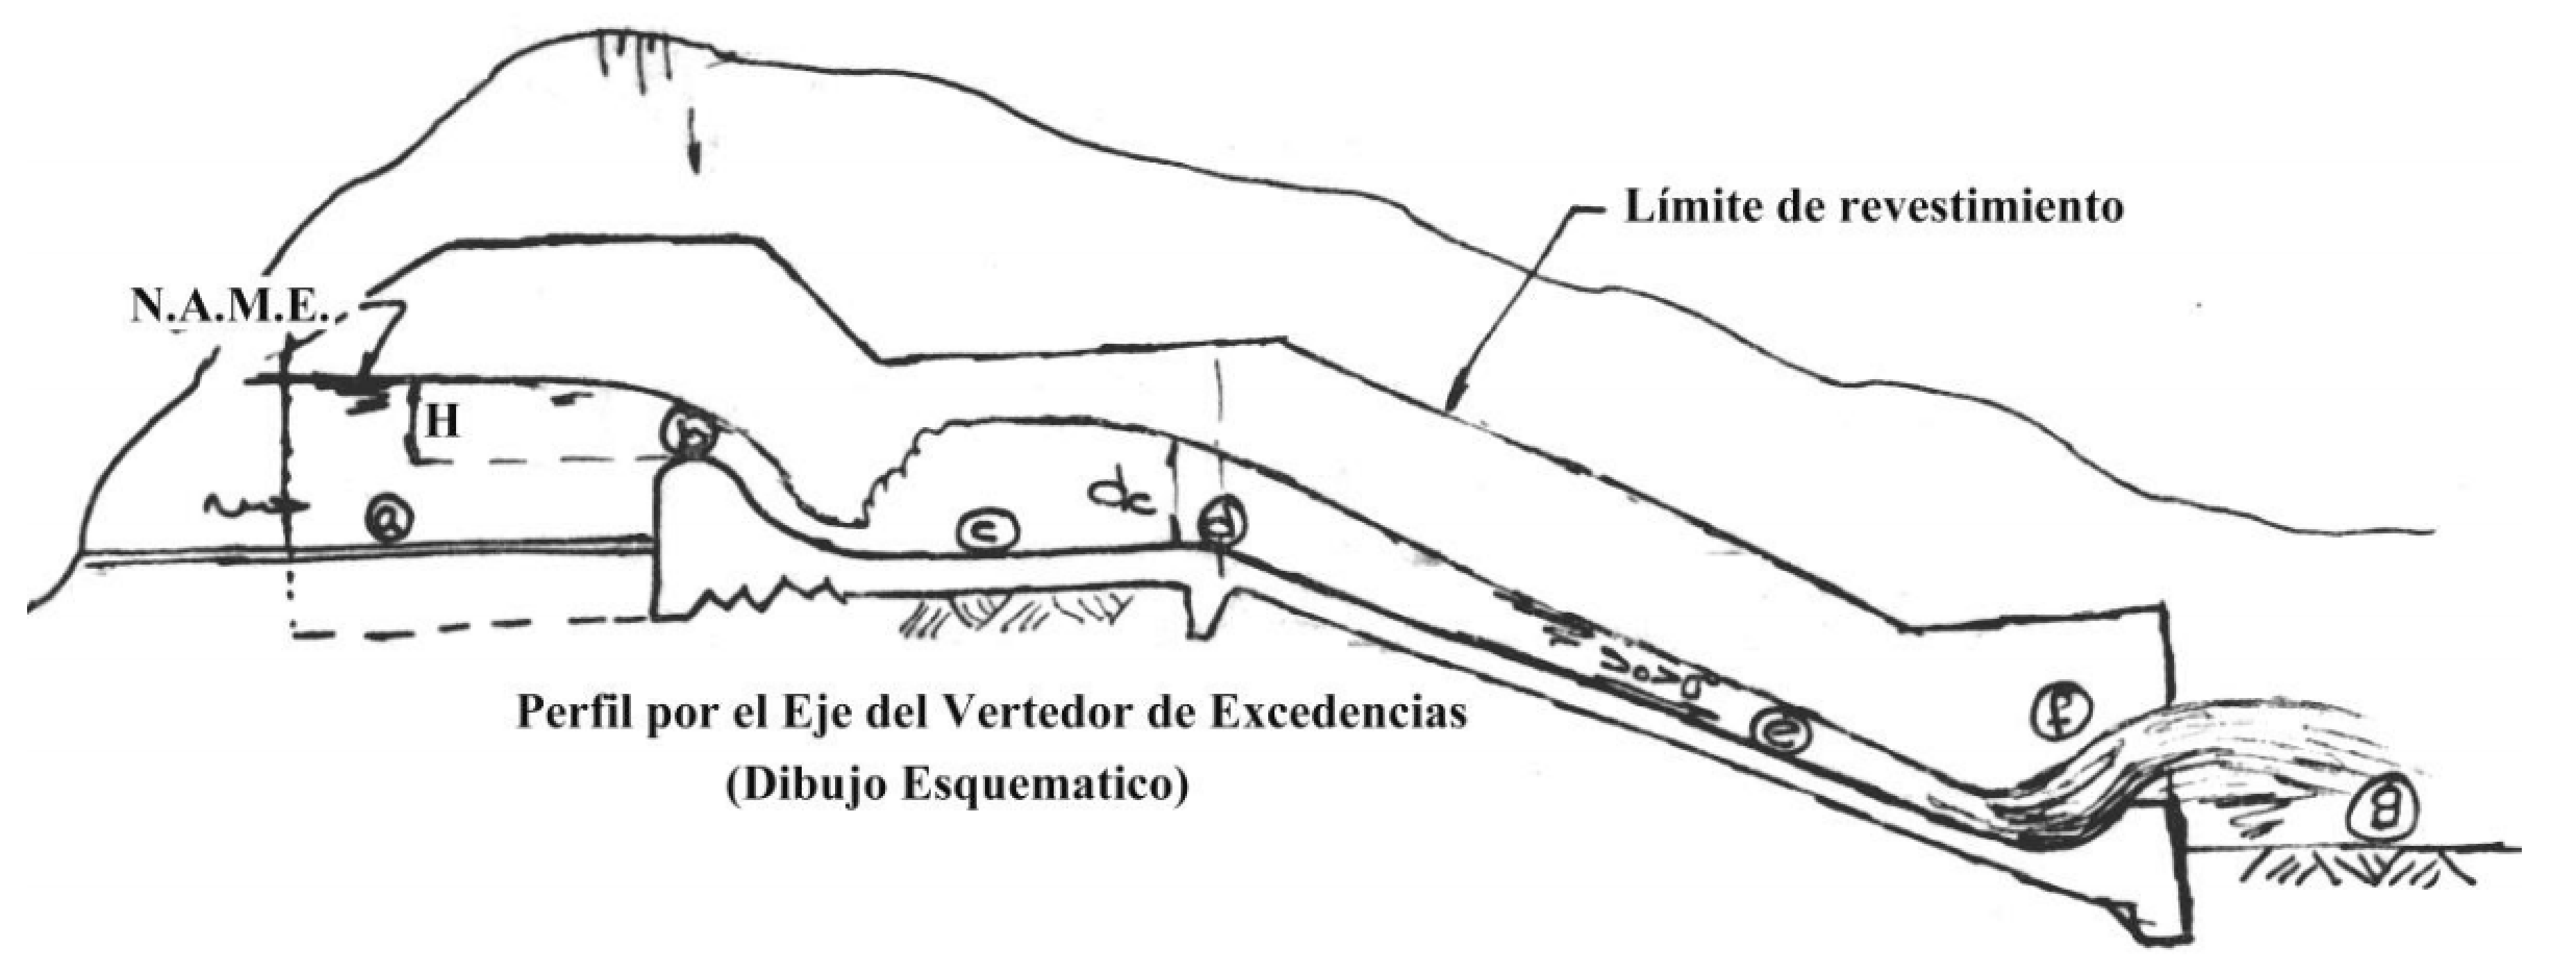
\includegraphics[width=0.5\textwidth]{fii49.png}}
	\caption{Partes que conforman a una obra de excedencias.}
	\label{fii49}
\end{figure}

\subsubsection{Localización de la obra de excedencias.}

\begin{enumerate}[noitemsep]
	\item En el cuerpo de la cortina: Esta localización solo se puede tener cuando la presa es rígida, aprovechando
	      sus características que permiten que una estructura rígida se aloje en otra similar.
	      \begin{figure}[h!]
		      \centerline{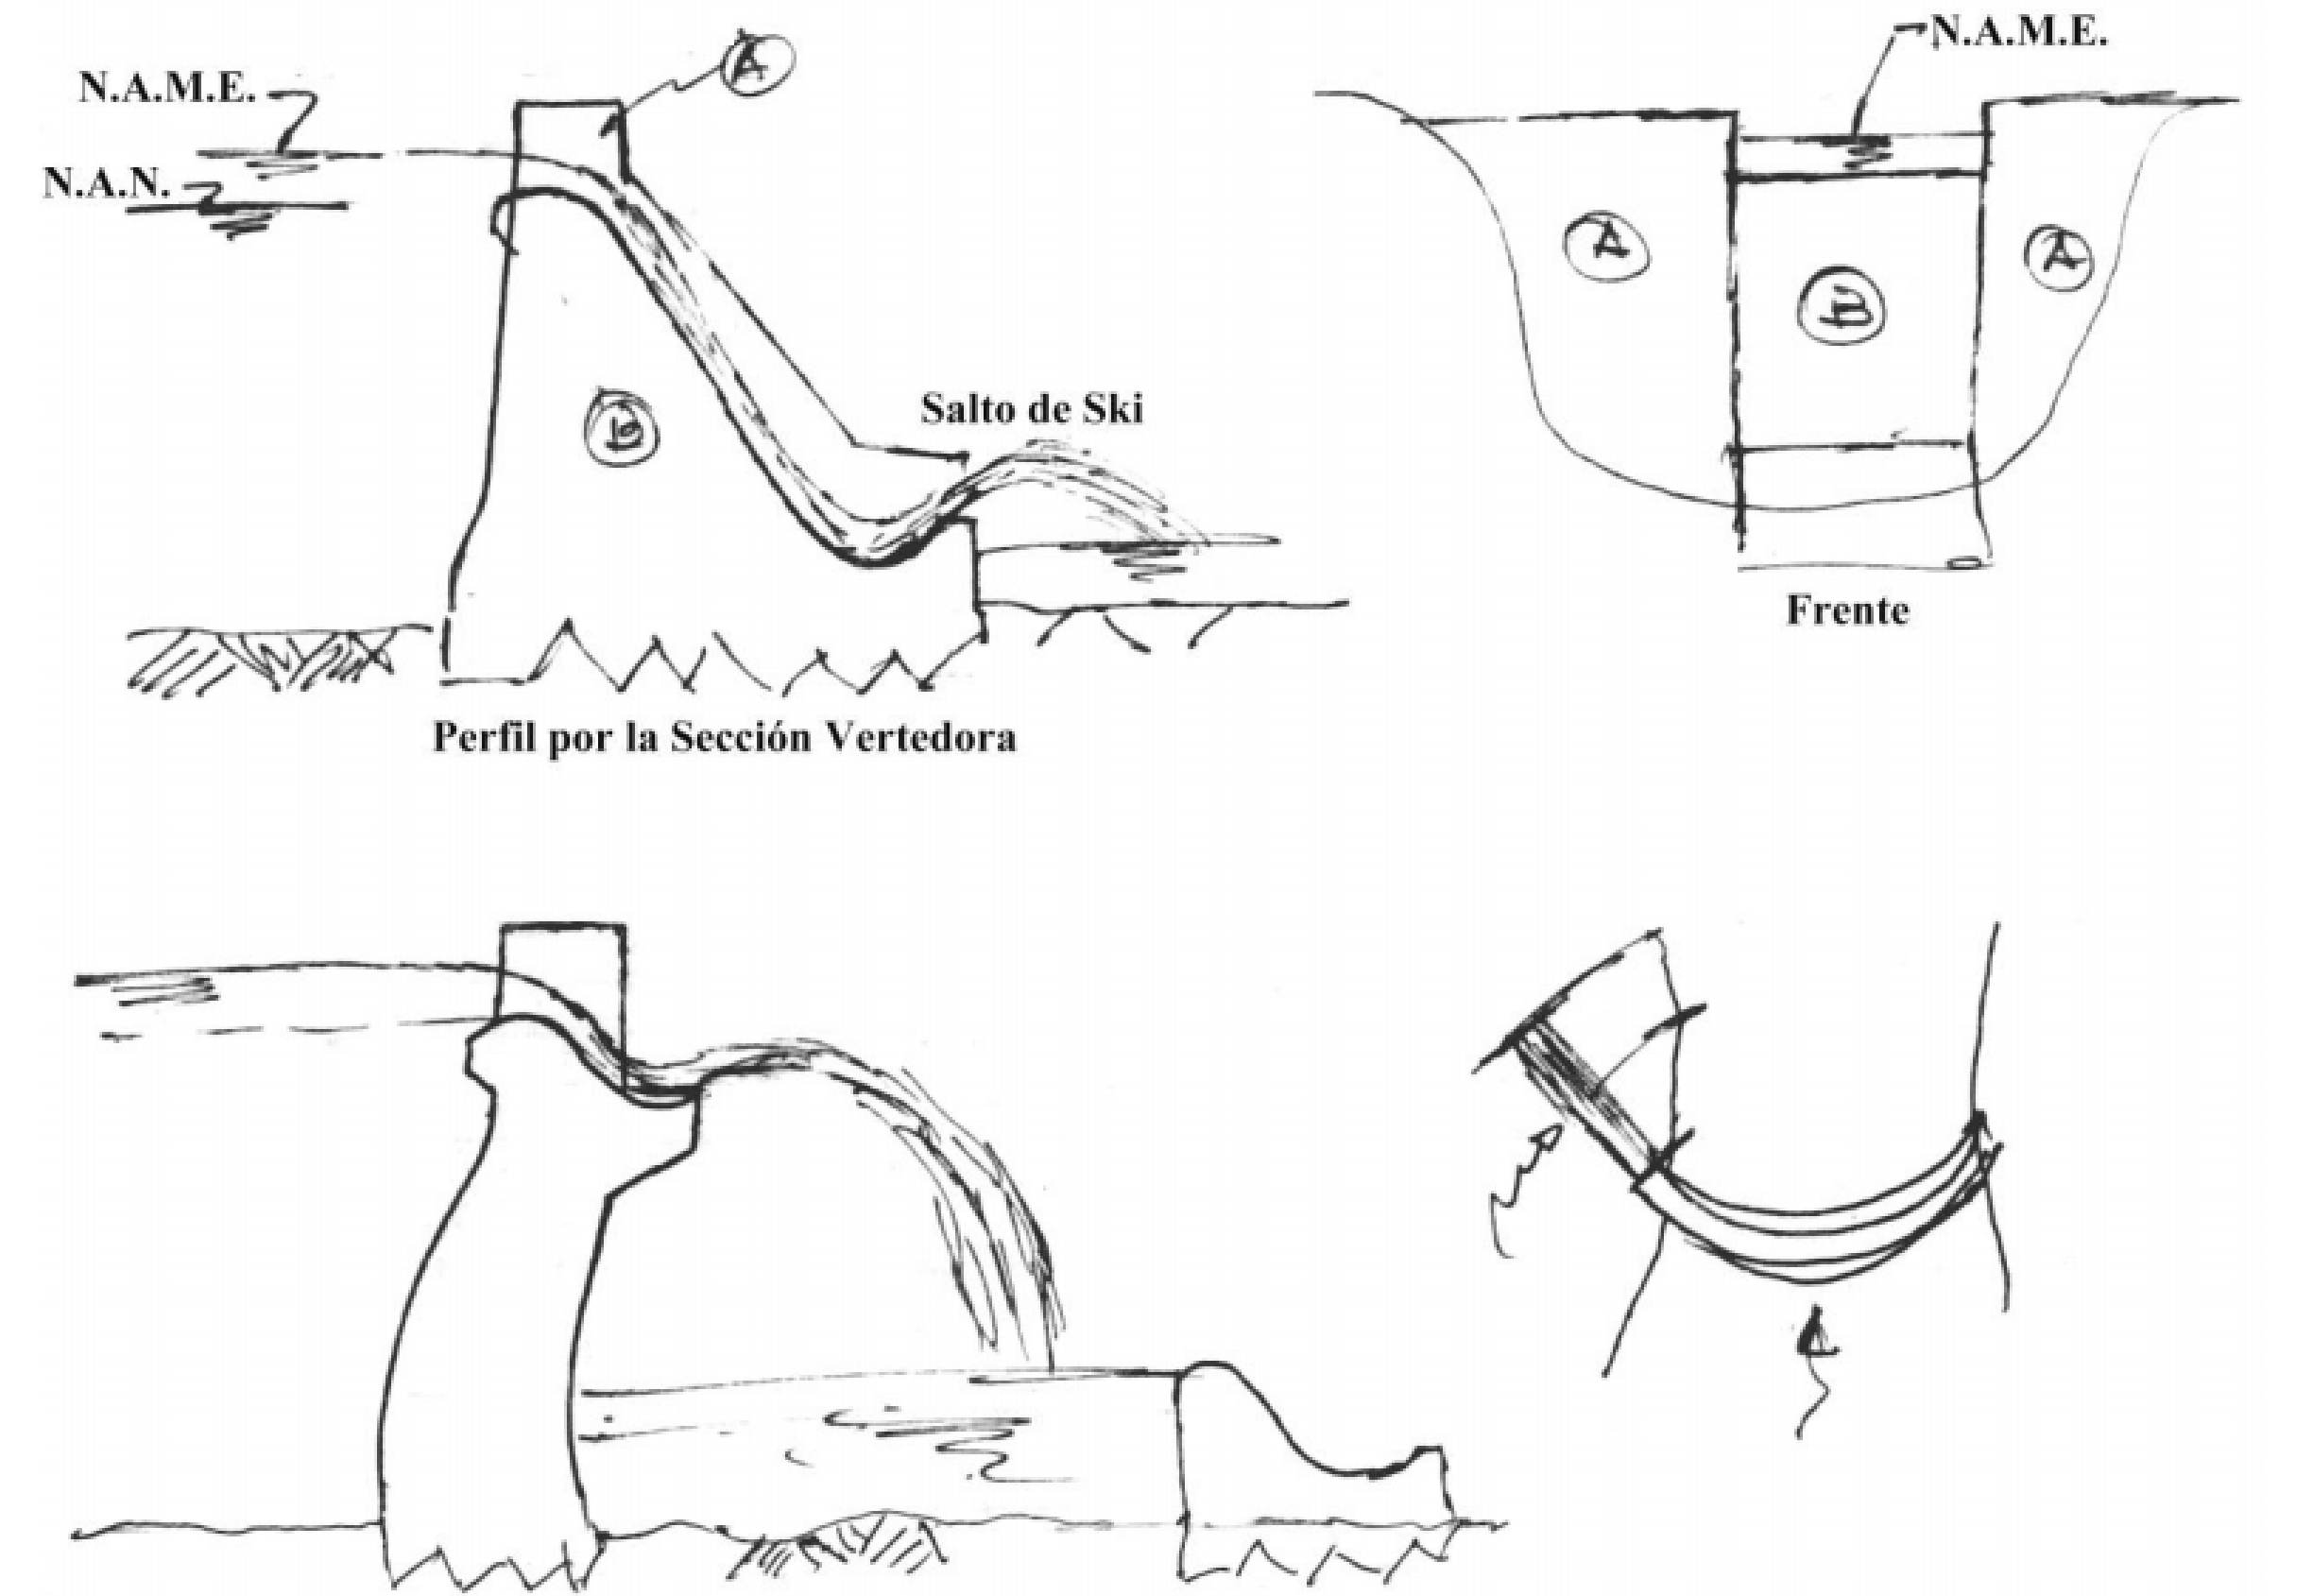
\includegraphics[width=0.5\textwidth]{fii50.png}}
		      \caption{Esquemas de localización de la obra de excedencias en el cuerpo de la
			      cortina.}
		      \label{fii50}
	      \end{figure}
	\item En las laderas
	\item En puerto natural
	      \begin{figure}[h!]
		      \centerline{\includegraphics[width=0.5\textwidth]{fii51.png}}
		      \caption{Esquemas de localización de obras de excedencias en ladera y puerto
			      natural.}
		      \label{fii51}
	      \end{figure}
\end{enumerate}

\subsubsection{Factores que afectan a las obras de excedencias y que
	determinan el tipo.}

\begin{itemize}
	\item Topografía
	\item Geología
	\item Tipo de cortina
	\item Régimen de la corriente
	\item Economía
\end{itemize}

\subsubsection{Diversos tipos de vertedores.}

Existen diversos criterios para clasificar a las obras de excedencias:

\begin{enumerate}[noitemsep]
	\item Por su localización
	      \begin{enumerate}
		      \item Vertedores en el cuerpo de la cortina
		      \item Vertedores en la ladera
		      \item Vertedor en puerto natural
	      \end{enumerate}
	\item Por la forma de descarga
	      \begin{enumerate}
		      \item Vertedores de descarga libre
		      \item Vertedores de descarga controlada por medio de compuerta
	      \end{enumerate}
	\item Por la forma del eje de la estructura de control
	      \begin{enumerate}
		      \item Vertedores de cresta recta
		      \item Vertedores de cresta curva
		      \item Vertedores de cresta combinada
	      \end{enumerate}
	\item Por la posición del canal de descarga
	      \begin{enumerate}
		      \item Vertedor con canal de descarga normal a la cresta
		      \item Vertedor con canal de descarga paralelo a la cresta
	      \end{enumerate}
\end{enumerate}

\subsubsection{Tipos de vertedores de excedencias comunes:}

\begin{enumerate}[noitemsep]
	\item Vertedores de descarga directa
	      \begin{enumerate}
		      \item Cresta recta
		            \begin{enumerate}
			            \item Lavadero
			            \item Cimacio
			                  \begin{enumerate}
				                  \item Creager
				                  \item Scimeni
			                  \end{enumerate}
			            \item Cresta curva
			                  \begin{enumerate}
				                  \item Abanico
				                  \item Medio abanico
			                  \end{enumerate}
		            \end{enumerate}
	      \end{enumerate}
	\item De canal lateral
	\item De cresta controlada (movil)
\end{enumerate}

\begin{figure}[h!]
	\centerline{\includegraphics[width=0.5\textwidth]{fii52.png}}
	\caption{Esquemas de vertedores de excedencias cresta recta y cresta curva.}
	\label{fii52}
\end{figure}


\subsection{Sistema de derivación.}

\begin{definition}[Sistema de derivación]
	es aquel que tiene por objeto aprovechar las aguas
	superficiales en forma controlada y sin alterar el régimen de la fuente de
	abastecimiento, en una disposición tal que se puedan conducir hasta el sitio de
	utilización, ya sea por gravedad o por bombeo.
\end{definition}

Cuando se tiene que el gasto de la corriente es mayor o igual que el gasto que
las necesidades de la demanda plantea, se exige la construcción de una obra de
derivación, y cuando es menor lo que se plantea es una obra de almacenamiento.
Las fuentes de abastecimiento que se aprovechan para construir este tipo de
obras principalmente son: Arroyos, ríos, lagunas y manantiales. Como en algunas
ocasiones se combina la captación de los escurrimientos superficiales con la de las
aguas subálveas y por ello algunas obras, como las galerías filtrantes pueden quedar
incluidas en las obras de derivación.
Considerando las características, tanto de la fuente de abastecimiento como de
la obra, y de acuerdo a lo anterior, básicamente se tienen los siguientes tipos de obras
de derivación.

\begin{itemize}
	\item Tomas directas
	\item Barrajes simples
	\item Presas derivadoras
	\item Captación en manantiales
	\item Galerías filtrantes
	\item Diques subterráneos
	\item Plantas de bombeo.
\end{itemize}

En este texto solo se van a analizar las presas derivadoras y posteriormente las plantas
de bombeo.

\begin{definition}[presa derivadora]
	es aquella estructura hidráulica que se proyecta y
	construye en un cauce y que tiene por objeto aprovechar las aguas superficiales que se
	presentan en el mismo, en forma controlada y sin alterar el régimen del escurrimiento,
	en una disposición tal que se puedan conducir hasta el sitio de utilización, ya sea por
	gravedad o por bombeo.
\end{definition}

Cuando se tiene que el gasto de la corriente es mayor o igual que el gasto que
las necesidades de la demanda plantea, se exige la construcción de una obra de
derivación, y cuando es menor lo que se plantea es una obra de almacenamiento.
Las estructuras que se pueden presentar en una presa derivadora son:
\textbf{esenciales} y \textbf{auxiliares}.

\begin{enumerate}
	\item Estructuras esenciales de una presa derivadora
	      \begin{enumerate}
		      \item Cortina
		            \begin{figure}[h!]
			            \centerline{\includegraphics[width=0.5\textwidth]{fii53.png}}
			            \caption{Planta esquemática de bocatoma y canal desarenador de presa derivadora.}
			            \label{fii53}
		            \end{figure}
		      \item Bocatoma
		            \begin{figure}[h!]
			            \centerline{\includegraphics[width=0.5\textwidth]{fii54.png}}
			            \caption{Perfil esquemático de canal desarenador y bocatoma de presa derivadora.}
			            \label{fii54}
		            \end{figure}
		      \item canal desarenador
		            \begin{figure}[h!]
			            \centerline{\includegraphics[width=0.5\textwidth]{fii55.png}}
			            \caption{Perfil esquemático de canal de conducción, bocatoma, canal desarenador y dique derivador de una presa derivadora.}
			            \label{fii55}
		            \end{figure}
	      \end{enumerate}
	\item Estructuras Auxiliares de una presa derivadora
	      \begin{enumerate}
		      \item Bordo de Protección
		      \item Escala para peces
		            \begin{figure}[h!]
			            \centerline{\includegraphics[width=0.5\textwidth]{fii56.png}}
			            \caption{Perfil esquemático de escala para peces en presa derivadora.}
			            \label{fii56}
		            \end{figure}
		      \item Esclusas para navegación
		            \begin{figure}[h!]
			            \centerline{\includegraphics[width=0.5\textwidth]{fii57.png}}
			            \caption {Planta y perfil esquemático de esclusas y canal de navegación en presa derivadora.}
			            \label{fii57}
		            \end{figure}
		      \item Pasos para troncos
		            \begin{figure}[h!]
			            \centerline{\includegraphics[width=0.5\textwidth]{fii58.png}}
			            \caption {Planta y perfil esquemático de paso para troncos en presa derivadora.}
			            \label{fii58}
		            \end{figure}
	      \end{enumerate}
\end{enumerate}

\subsection{Clasificación de cortinas de derivación}

\begin{enumerate}
	\item a)Respecto a su planta
	      \begin{enumerate}
		      \item Planta curva
		      \item Planta recta
	      \end{enumerate}
	\item Referente a las líneas de corriente
	      \begin{enumerate}
		      \item  Eje normal
		      \item  Eje esviajado
	      \end{enumerate}
	\item Respecto al flujo de las avenidas
	      \begin{enumerate}
		      \item cortinas vertedoras
		      \item Cortinas no vertedoras
	      \end{enumerate}
	\item En relación a la carga sobre la cresta
	      \begin{enumerate}
		      \item Cresta controlada
		      \item Cresta sin control
	      \end{enumerate}
	\item Según los materiales empleados
	      \begin{enumerate}
		      \item Cortinas rígidas
		            \begin{enumerate}
			            \item Concreto
			            \item Mampostería
		            \end{enumerate}
		      \item Cortinas flexibles
		            \begin{enumerate}
			            \item Enrocamiento
		            \end{enumerate}
		      \item Cortinas mixtas
	      \end{enumerate}
	\item Según el terreno de la cimentación
	      \begin{enumerate}
		      \item Cimentación en roca
		      \item Cimentación en material de acarreo
	      \end{enumerate}
\end{enumerate}

\begin{figure}[h!]
	\centerline{\includegraphics[width=0.5\textwidth]{fii59.png}}
	\caption{Dique derivador o cortina flexible tipo indio de presa derivadora.}
	\label{fii59}
\end{figure}

\subsection{Descripción de las partes de una presa derivadora}

\subsubsection{Dique derivador o cortina de excedencias.}

El dique derivador o cortina de excedencias es un dique que tiene por objeto
levantar el nivel de la superficie libre del agua que escurre en un cauce de río o arroyo a
fin de poder extraerla y llevarla por gravedad a la zona de riego, y cuando se presenten
avenidas facilitar el que puedan pasar por encima de el y entregarla al mismo cauce
donde se encuentra.

\subsubsection{Bocatama}

La bocatoma en una presa derivadora es aquella estructura que permite desviar
y entregar al canal de conducción los escurrimientos que desean ser aprovechados en
los beneficios para los cuales se ha proyectado y construido la presa derivadora.

\subsubsection{Canal desarenador.}

El canal desarenador en una presa derivadora es aquella parte de la misma que
tiene por objeto mantener limpio el acceso a la bocatoma libre de obstáculos que
pongan en peligro la operación de esta, evitando a la vez el que materiales en
suspensión y/o arrastre puedan ser conducidos al canal de conducción, evitando la
obstrucción de la bocatoma o el azolvamiento de la sección del canal.

\subsection{Sistema de conducción y distribución}

\begin{definition}[sistema de conducción y distribución]
	Es el conjunto de canales y sus
	estructuras, las cuales se requieren para conducir y distribuir el agua proveniente de la
	fuente de abastecimiento, en todos los lotes o parcelas que conforman a la zona de
	riego.
\end{definition}

\subsubsection{Elementos del sistema.}

\begin{itemize}
	\item Canales. Conductos por los cuales se hace circular por gravedad el agua, para
	      transportarla desde la fuente de abastecimiento hasta los lotes o parcelas de
	      riego.
	\item Estructuras. Obras de arte necesarias para conducir el agua de una sección o
	      nivel a otro (a), cruzar obstáculos diversos, controlarla y distribuirla, así como
	      proteger el sistema.
\end{itemize}

\subsection{Clasificación de canales.}

\begin{definition}[Canal Principal (CP).]
	Es aquel que domina toda el área regable y abastece el
	sistema de canales laterales.
\end{definition}

\subsubsection{Canales Secundarios}

\begin{definition}[ Canal lateral (CL).]
	Es el canal que domina las divisiones principales del área
	regable y abastece a los sublaterales.
\end{definition}

\begin{definition}[Canal Sublateral (CSL).]
	Son necesarios para ramificar un lateral en dos o
	más canales.
\end{definition}

\begin{definition}[ Ramal (CR).]
	Es abastecido por un sublateral y a su vez abastece a los
	subramales (cuando existen) o a las regaderas (últimas ramificaciones de la red de
	distribución).
\end{definition}

En todos los canales se pueden tener tomas para el riego directo de los lotes, en
cuyo caso se denominan tomas granja.

\subsubsection{Canales no revestidos contra canales revestidos.}

Cuando el material natural en el que se aloje la sección de un canal presente
permeabilidades menores a $3x10^{-5} \frac{cm}{seg}$ los canales no deben revestirse, en caso
contrario es conveniente analizar la conveniencia técnico económica de planear un
revestimiento.

\subsubsection{Secciones de canales sin revestimiento.}

Las secciones de canales en tierra sin revestimiento se usan en zonas de suelos
arcillosos pesados, en los que la pérdida de agua por infiltración es mínima y no se
justifica su revestimiento por alguna razón.

Las pérdidas de agua que pueden tenerse en un canal en tierra se pueden
clasificar en inevitables y susceptibles de evitarse o disminuirse.

\begin{enumerate}
	\item Pérdidas inevitables
	      \begin{enumerate}
		      \item Evaporación
	      \end{enumerate}
	\item Pérdidas susceptibles de evitarse
	      \begin{enumerate}
		      \item Pérdidas de conducción en canales: infiltración, transpiración de la vegetación en bordos o en la sección del canal
		      \item Pérdidas en la operación de estructuras.
	      \end{enumerate}
\end{enumerate}

Factores que afectan la infiltración en canales sin revestimiento:

\begin{itemize}
	\item Textura y estructura del suelo
	\item Contenido de sólidos en suspensión en el agua que conducen los canales y velocidad de sedimentación
	\item Relación de las dimensiones del canal al gasto Capilaridad del material
	\item Posición del nivel freático respecto del canal.
\end{itemize}

En resumen, las pérdidas por infiltración en canales excavados en tierra, se
deben a presiones hidrostáticas, fuerza de gravedad, temperatura del agua y suelo, así
como tensiones capilares combinadas con los factores enunciados, variando a lo largo
de cada canal, conforme cambian los factores que intervienen definiendo la
permeabilidad en bordos y plantilla

\subsubsection{Revestimiento de canales.}
Un revestimiento de canales consiste en dotarle a la sección de los mismos de
una cobertura artificial conformada con un material determinado, comúnmente concreto
simple, que permita reducir o atenuar las pérdidas por filtración en la sección.

\textbf{Tipos de revestimiento:}

\begin{enumerate}
	\item Revestimiento de superficie dura
	      \begin{enumerate}
		      \item Concreto reforzado o simple, colado en el sitio o precolado en losas y bloques
		      \item Gunita (mortero aplicado neumáticamente)
		      \item Suelo-cemento
		      \item Concreto asfáltico, colado en el sitio o precolado
		      \item Mampostería de piedra o tabique
	      \end{enumerate}
	\item  Revestimiento de membrana expuesta
	      \begin{enumerate}
		      \item Membrana asfáltica
		      \item Película de plástico y hule sintético
	      \end{enumerate}
	\item  Revestimiento de membrana enterrada
	      \begin{enumerate}
		      \item Membrana asfáltica aplicada en el sitio
		      \item Película de plástico y hule sintético
		      \item Membrana asfáltica prefabricada
		      \item Membrana de Bentonita
	      \end{enumerate}
	\item  Revestimiento de tierra
	      \begin{enumerate}
		      \item Revestimiento de tierra compactada
		      \item Colchones de tierra suelta
		      \item Mezcla de suelos
		      \item Mezcla de suelos con aditivos
	      \end{enumerate}
\end{enumerate}

\subsection{Efectos de un revestimiento}

Los principales resultados del revestimiento de canales son:

\begin{enumerate}
	\item Mejoramiento de características hidráulicas con respecto a canales de tierra
	\item Evita la ruptura de bordos y fugas de agua a través de tuceras
	\item Estabiliza la sección del canal
	\item Permite mayores pendientes
	\item Reduce el número y tamaño de las estructuras
	\item Ahorro de agua
	\item Restauración al uso agrícola de tierras empantanadas y ensalitradas por infiltración
	\item Reduce el costo de drenaje
	\item Reduce el costo de operación y mantenimiento
\end{enumerate}

\subsubsection{Selección del tipo de Revestimiento.}

Los factores que determinan la selección del tipo de revestimiento son:

\begin{enumerate}
	\item Pérdidas por percolación
	\item Costos anuales de conservación
	\item Velocidad media baja en el canal, que por razones económicas hay que aumentar
\end{enumerate}

\subsection{Localización de canales.}

\subsubsection{Canales principales.}

La localización de canales principales, cuando su origen es una presa de
almacenamiento o una presa derivadora, deberá hacerse siguiendo aproximadamente
una curva de nivel de manera que se domine la mayor superficie posible de tierras.

De acuerdo a la topografía se presentan dos casos generales: 1) cuando el
terreno tiene una topografía plana o ligeramente ondulada, y 2) Cuando el terreno
presenta una topografía muy movida, llegando en algunos casos a ser extremadamente
abrupta.

Los canales principales se localizan dependiendo si se refieren a tramos de
conducción o en tramo de distribución dentro de la zona de riego, el segundo se traza
considerando una sección compensada que permita brindar dominancia de riego esto
es que la \textbf{Superficie Libre del Agua} en el canal (SLA) se ubique por arriba del terreno
natural, el primero puede ser localizado considerando una sección enterrada

\begin{figure}[h!]
	\centerline{\includegraphics[width=0.5\textwidth]{fii60.png}}
	\caption {Secciones tipo en tramos de canal principal en zona de distribución y en tramos de conducción.}
	\label{fii60}
\end{figure}

\subsection{Canales secundarios}

Los canales secundarios son los que conforman la red de distribución, los cuales
son: Canal lateral, canal sublateral, canal ramal, canal subramal y las regaderas.
Existen cuatro criterios generales a seguir en la localización de canales
secundarios:

\subsubsection{Según la topografía del terreno:}
Este es el más económico, ya que los canales se localizan por el parteaguas y
van dominando hacia ambos lados del canal, resultando la red de distribución más
corta. Además, que se aprovechan los talwegs para alojar los drenes. El inconveniente
es que resultan lotes irregulares.

\subsubsection{Localización según la cuadricula:} Este es privativo de terrenos de gran extensión, de topografía muy plana y de
poca pendiente y cuando el procedimiento de levantamiento ha sido una cuadricula. Se
facilita grandemente el trazo en el campo resultando lotes regulares de las extensiones
que sean autorizadas. Este método presenta la ventaja de facilitar la operación y
conservación del sistema de riego. El inconveniente, es que resulta la red más larga
que en el anterior procedimiento, al regar solamente hacia un lado, se requieren más
tomas y estructuras adicionales requiriéndose la construcción alternada de un dren y un
canal.

\subsubsection{Localización respetando los linderos. }

En ocasiones cuando ya existen linderos de propiedad es necesario localizar los
canales laterales siguiendo estos, en tanto la topografía lo permita. El costo de la
construcción, operación y conservación es muy variable, dependiendo de la extensión y
forma de las propiedades.

\subsubsection{Localización según un sistema combinado.}

Este sigue los tres anteriores sistemas. Siendo este el más conveniente.

\subsection{Localización de tomas granja y caídas}

Una toma granja es una estructura en los canales que permite hacer la
extracción del agua en forma controlada y segura para entregarla a las regaderas (canal
que permite distribuir el agua al interior de lotes o parcelas de riego).
Caída es una estructura en los canales que permite salvar los desniveles que se
van acumulando con la diferencia entre las pendientes del canal y la natural del terreno
en tanto la diferencia no sea mayor a 4 m y esta se verifique en una distancia
relativamente corta.

\begin{figure}[h!]
	\centerline{\includegraphics[width=0.5\textwidth]{fii61.png}}
	\caption{Esquemas de localización de canales secundarios.}
	\label{fii61}
\end{figure}

\subsection{Localización de Tomas Granja (T.G.).}

Se deben seguir las siguientes reglas fundamentales:

\begin{enumerate}
	\item La rasante de la regadera a la salida de la toma debe ser tal, que sin elevar el
	      nivel de la S.L.A. en el canal alimentador, sea posible colocar el agua en el terreno
	      que vaya a regar.
	\item  El desnivel entre las S.L.A. del canal alimentador y regadera, debe ser de 10
	      cm mínimo (pérdida de carga en la T.G.)
	\item  La S.L.A. a la salida de la toma debe quedar 30 cm mínimo, arriba del Terreno
	      Natural.
	\item El desnivel mínimo entre las S.L.A. del canal alimentador y la superficie del
	      terreno a la salida de la toma debe ser de 40 cm.
	\item Para garantizar que la toma trabaje ahogada siempre, se baja la plantilla de la
	      tubería un mínimo de 40 cm.
\end{enumerate}

\begin{figure}[h!]
	\centerline{\includegraphics[width=0.5\textwidth]{fii62.png}}
	\caption{Elementos de localización de tomas granja}
	\label{fii62}
\end{figure}

\subsubsection{Localización de caídas}

Se deben seguir las siguientes normas:

\begin{enumerate}
	\item El costo por metro lineal de canal, incluyendo excavaciones, préstamos,
	      costos de caídas y costo de represas adicionales que sea necesario construir, deberá
	      ser mínimo.
	\item Las caídas serán verticales y se localizarán de preferencia en los sitios en que
	      sea necesario construir represas o tomas, en tanto no representen costos elevados los
	      refuerzos del muro vertical debido al empuje de tierras, sino de preferencia se
	      recomiendan sean inclinadas.
	\item Debe procurarse uniformizar la altura de caída en cada proyecto.
\end{enumerate}

\subsubsection{Estructuras de conducción.}

Las estructuras de conducción en canales son aquellas que permiten unir dos
tramos de canal con diferente sección o con diferente nivel. Las estructuras se
conducción se clasifican en: Transiciones, caídas y rápidas. Las transiciones pueden
ser: Biplanares, regladas y alabeadas. Las caídas son: verticales e inclinadas.

\begin{figure}[h!]
	\centerline{\includegraphics[width=0.5\textwidth]{fii63.png}}
	\caption{Esquemas de transiciones en canales.}
	\label{fii63}
\end{figure}

\begin{figure}[h!]
	\centerline{\includegraphics[width=0.5\textwidth]{fii64.png}}
	\caption{Esquemas de caídas y rápida.}
	\label{fii64}
\end{figure}

\subsubsection{Estructuras de cruce}

Las estructuras de cruce en canales son aquellas que permiten salvar obstáculos
diversos que en el desarrollo del canal se van encontrando, tales como arroyos, ríos,
caminos, FFCC, otro canal o un dren.
Las estructuras de cruce pueden ser: Sifones, Puentes canal, alcantarillas o
puentes para camino o FFCC.

\subsubsection{Estructuras de control y distribución.}

Las estructuras de control y distribución en canales son aquellas que permiten
controlar los niveles y gastos en los canales para poder distribuir el agua hacia otros
canales o a las parcelas o lotes de riego.
Las estructuras de control y distribución se clasifican en: Represa, repartidores,
tomas y estructuras aforadoras. Las tomas pueden ser: para canal o granjas

\subsubsection{Estructuras de protección.}

Las estructuras de protección en canales son aquellas que permiten proteger a
los canales contra los escurrimientos laterales de ladera, así como para cuando se
tienen elevaciones peligrosas de la superficie libre del agua en los mismos.

Las estructuras de protección pueden ser: Desfogues, cunetas y contracunetas,
entradas de agua, pasos superiores y pasos inferiores. Los desfogues pueden ser a su
vez, en desfogues de excedencias o limitadores de gasto y desfogues totales.

\begin{figure}[h!]
	\centerline{\includegraphics[width=0.5\textwidth]{fii65.png}}
	\caption{Esquemas de desfogues y entradas de agua}
	\label{fii65}
\end{figure}

\begin{figure}[h!]
	\centerline{\includegraphics[width=0.5\textwidth]{fii66.png}}
	\caption{Esquema de cunetas y contracunetas, paso superior y paso inferior.}
	\label{fii66}
\end{figure}


\subsection{Sistema de drenaje.}

\begin{definition}[Sistema de drenaje]
	Es el conjunto de obras que permiten mantener el nivel freático en una zona de
	riego por debajo de la zona radicular de los cultivos con el fin de evitar daños a los
	suelos (en su estructura y otras características), y a los cultivos, asi como drenar las
	agua pluviales que se presentan en la zona.
\end{definition}

\subsubsection{Clasificación del sistema de drenaje}

\begin{enumerate}
	\item Drenaje Natural
	\item Drenaje Artificial
	      \begin{enumerate}
		      \item Superficial
		            \begin{enumerate}
			            \item Canales abiertos
			            \item Principales
			            \item Colectores
			            \item Primarios
			            \item Secundarios
			            \item Parcelarios
		            \end{enumerate}
		      \item Subterráneo
		            \begin{enumerate}
			            \item Drenes por medio de tubo
			            \item Drenes topo
			            \item Drenaje por bombeo
			            \item Drenaje parcelario (entubado)
		            \end{enumerate}
	      \end{enumerate}
\end{enumerate}

\subsubsection{Drenaje superficial o abierto}

\begin{figure}[h!]
	\centerline{\includegraphics[width=0.5\textwidth]{fii67.png}}
	\caption{Esquemas del sistema de drenaje.}
	\label{fii67}
\end{figure}

Las obras de drenaje a cargo de la administración de la zona de riego es la que
se refiere al drenaje superficial: Principales y colectores, primarios, secundarios, etc., y
las obras a cargo del usuario es lo que se refiere al drenaje parcelario, comúnmente
subterráneo, como drenes topo y drenes por medio de tubos

\subsubsection{Drenaje subterráneo o interno}

\begin{figure}[h!]
	\centerline{\includegraphics[width=0.5\textwidth]{fii68.png}}
	\caption{Alternativas de drenaje interno o subterráneo.}
	\label{fii68}
\end{figure}

\subsubsection{Descarga de drenes}

\begin{figure}[h!]
	\centerline{\includegraphics[width=0.5\textwidth]{fii69.png}}
	\caption{Esquemas de estructuras de desagüe, en sistemas de drenaje.}
	\label{fii69}
\end{figure}

\subsection{Sistema de comunicaciones y obras auxiliares}

\begin{definition}[Sistema de comunicaciones y obras auxiliares]
	El sistema de comunicaciones es el conjunto de obras y estructuras que permiten
	la transportación de los productos, y primordialmente la conservación y comunicación
	de las obras de la zona de riego, de acuerdo con las condiciones de funcionamiento
	óptimo para las que fueron proyectadas y construídas.
\end{definition}

\begin{figure}[h!]
	\centerline{\includegraphics[width=0.5\textwidth]{fii71.png}}
	\caption{Esquema del sistema de comunicaciones.}
	\label{fii71}
\end{figure}

\subsubsection{Caminos de Servicio}

\begin{enumerate}
	\item Sistema general de caminos del distrito o zona de riego
	\item Caminos sobre los bordos de los canales de riego y drenaje
	\item Caminos de acceso a obras especiales y dependientes del distrito o zona de riego.
\end{enumerate}


\subsubsection{Red telefónica interior}

Es necesario establecer una pronta comunicación entre las zonas clave de una
zona de riego y las oficinas centrales, haciéndose imperiosa la adquisición e instalación
de un sistema telefónico para satisfacer y garantizar la intercomunicación de los puntos
señalados.


Un sistema telefónico debe conectar, por medio de una red de casetas, las
diversas partes que componen a una zona de riego (obras de almacenamiento,
derivación, distribución y protección).

\subsubsection{Caminos Canaleros}

\begin{figure}[h!]
	\centerline{\includegraphics[width=0.5\textwidth]{fii70.png}}
	\caption{Esquemas de caminos canaleros en zonas de riego.}
	\label{fii70}
\end{figure}

\section{Plantas y equipos de bombeo.}

En todos los casos en que el terreno de riego quede por arriba de la S.L.A., en la
fuente de abastecimiento, o el sistema de riego, por sus características de los
elementos de conducción, distribución y aplicacion, son de alta presurización, se hace
necesario tener algún tipo de bombeo.

Para poder definir las características de las plantas y equipos de bombeo se
requiere definir el origen de las aguas para poder efectuar el bombeo.
Dependiendo del origen de las aguas del bombeo, se pueden tener:
\begin{enumerate}
	\item Aprovechamiento de aguas superficiales por bombeo:
	      Plantas de Bombeo en: Almacenamientos, escurrimientos naturales (arroyos o ríos),
	      escurrimientos artificiales (canales) o en lagos y lagunas.
	\item Aprovechamiento de aguas subsuperficiales por bombeo:
	      Pozos someros o galerías.
	\item Aprovechamiento de aguas subterráneas por bombeo:
	      Pozos profundos o galerías.
\end{enumerate}

\subsection{Aprovechamientos de aguas superficiales por bombeo.}

\subsubsection{Tipos de plantas de bombeo}
\begin{enumerate}
	\item Plantas de Bombeo sobre ríos o arroyos de carácter permanente
	\item Plantas de Bombeo en embalses artificiales y naturales
	\item Plantas de Bombeo en canales y drenes
	\item Plantas de Bombeo en manantiales y en cárcamos de bombeo
	\item Plantas de Bombeo con fines de drenaje
\end{enumerate}



\subsection{Elementos de una planta de bombeo.}

\begin{enumerate}
	\item Captación u obra de toma
	\item Cárcamo u obra de succión
	\item Equipo de bombeo
	\item Descarga
	\item Caseta de controles
	\item Subestación eléctrica o tanques de combustible
	\item Casa habitación del operador
	\item Obras auxiliares (cercos, caseta meteorológica, otras).
\end{enumerate}

\subsubsection{La captación u obra de toma}

Es la estructura mediante la cual se permite el acceso del agua hacia el cárcamo
de bombeo.

\begin{itemize}
	\item Canal de acceso o canal piloto
	\item Estructura de rejillas
	\item Medios de obturación
	\item Conducto hacia el cárcamo de bombeo.
\end{itemize}

Localización de obras de captación de plantas de bombeo.

\begin{figure}[h!]
	\centerline{\includegraphics[width=0.5\textwidth]{fii72.png}}
	\caption{Alternativas de localización recomendada de ubicación de obras de
		captación de plantas de bombeo en curvas de cauces.}
	\label{fii72}
\end{figure}


Estructura de Rejillas: pueden ser de concreto reforzado o mampostería
\begin{itemize}
	\item Permitir la instalación de rejillas.
	\item Posibilidad de tener un medio de obturación (abrir y cerrar el conducto)
\end{itemize}

\begin{figure}[h!]
	\centerline{\includegraphics[width=0.5\textwidth]{fii73.png}}
	\caption{Alternativas de obras de captación en plantas de bombeo.}
	\label{fii73}
\end{figure}

\begin{figure}[h!]
	\centerline{\includegraphics[width=0.5\textwidth]{fii74.png}}
	\caption{Casos típicos de plantas de bombeo.}
	\label{fii74}
\end{figure}

\begin{figure}[h!]
	\centerline{\includegraphics[width=0.5\textwidth]{fii75.png}}
	\caption{Disposición de los equipos de bombeo y accesorios en una planta de bombeo.}
	\label{fii75}
\end{figure}


\subsection{Aprovechamiento de las aguas subsuperficiales y subterráneas por bombeo.}

\subsubsection{Pozos Someros \textbf{Norias}}

\begin{figure}[h!]
	\centerline{\includegraphics[width=0.5\textwidth]{fii76.png}}
	\caption{Pozo ordinario, somero o tipo noria.}
	\label{fii76}
\end{figure}

\subsubsection{Construcción del pozo.}

En la construcción de pozos someros o tipo noria los diámetros de excavación
son de: $1.0 \leq  D \leq  5.0 m$, según necesidades particulares de cada excavación y a una
altura por etapas de acuerdo al material en el que se construye para evitar
desmoronamientos.

Las profundidades máximas a los que se construye los pozos tipo noria andan
entre: 25 y 30 m, para las cuales son más económicos en su construcción que en
diámetros pequeños.

Las secciones en planta para los que se construyen son:
\begin{itemize}
	\item Circulares (más usados)
	\item Rectangulares
	\item Elípticas
\end{itemize}

Estas dos últimas según la maquinaria elevadora.

\begin{figure}[h!]
	\centerline{\includegraphics[width=0.5\textwidth]{fii77.png}}
	\caption{Ubicación de la bomba en un pozo somero o tipo noria.}
	\label{fii77}
\end{figure}


\subsubsection{Aguas Subálveas.}
Las aguas subálveas son aquellas que se presentan por debajo del fondo de los cauces naturales, que sin presentarse un escurrimiento superficial quedan disponibles bajo un escurrimiento subsuperficial. Para aprovechar estas aguas es necesario construir una galería de filtración en el fondo del cauce para interceptar y captar esta agua y por gravedad llevarla a una de las márgenes, donde se construye un cárcamo de bombeo para extraer esas aguas y entregarlas a un canal de conducción, según se puede observar en la figura \ref{fii78}.

\begin{figure}[h!]
	\centerline{\includegraphics[width=0.5\textwidth]{fii78.png}}
	\caption{Esquema de galería de filtración y cárcamo de bombeo.}
	\label{fii78}
\end{figure}

\subsubsection{Aguas subterráneas.}
Las aguas subterráneas se pueden explotar en forma vertical a través de pozos
profundos o de pequeño diámetro el cual presenta como limitante a gastos limitados; o
en forma horizontal a través de galerías de filtración, para ser aprovechada el agua, ya
sea por gravedad o por bombeo.

\begin{figure}[h!]
	\centerline{\includegraphics[width=0.5\textwidth]{fii79.png}}
	\caption{Esquema de Pozo profundo.}
	\label{fii79}
\end{figure}

\begin{figure}[h!]
	\centerline{\includegraphics[width=0.5\textwidth]{fii80.png}}
	\caption{Esquema de una galería de filtración para explotación de las aguas subterráneas.}
	\label{fii80}
\end{figure}

\begin{figure}[h!]
	\centerline{\includegraphics[width=0.5\textwidth]{fii81.png}}
	\caption{Esquema de una galería de filtración para explotación de las aguas subterráneas.}
	\label{fii81}
\end{figure}

\subsection{Equipos de bombeo, instalaciones y accesorios.}

\subsubsection{Tipos de bombas}
\begin{enumerate}
	\item Bomba centrifuga (B.C.) de eje horizontal
	\item Bomba Centrifuga de eje vertical
	\item Bomba Turbina vertical para pozo profundo
	\item Bomba de Escurrimiento Mixto
	\item Bombas Axiales o de Propulsor.
\end{enumerate}

\begin{itemize}
	\item \textbf{Bomba centrifuga (B.C.) de eje horizontal.}
	      La Bomba Centrifuga de eje horizontal: se usa en explotaciones de aguas
	      superficiales (100,150 o 200 lps por unidad)

	\item \textbf{Bomba Centrifuga de eje vertical.}
	      La Bomba Centrifuga eje vertical, para funcionar en cárcamos, para galerías
	      filtrantes o pozos someros (preferible usar energía eléctrica).

	\item \textbf{Bomba turbina vertical para pozo profundo.}
	      Las Bombas turbinas verticales, que normalmente se usan para pozos
	      profundos, también pueden utilizarse en plantas de bombeo, presentan la facilidad de
	      poder tener acoplamientos para los dos tipos diferentes de energía (energía eléctrica y
	      combustión interna)

	\item \textbf{Bomba de escurrimiento mixto.}
	      Las Bombas de escurrimiento mixto, para gastos arriba de 100 lps (es una
	      Bomba turbina de eje vertical, pero de menos altura de carga y si grandes gastos).

	\item \textbf{Bombas axiales.}
	      Las Bombas Axiales o de Propulsor, pueden proporcionar gastos grandes (del
	      orden de m3/seg). Estas no deben trabajarse en pozos profundos o someros. Son
	      adecuadas para trabajarse en escurrimientos superficiales, o aprovechamientos de
	      poca altura o profundidad.
\end{itemize}


\subsubsection{Motores, casetas y habitaciones para el personal}

\begin{enumerate}
	\item Motores eléctricos y subestación
	\item Motores de combustión interna
	      \begin{enumerate}
		      \item Diesel
		      \item Gasolina
		      \item Combustóleo
		      \item Gas
		      \item Mixto
	      \end{enumerate}
\end{enumerate}

Las casetas y habitaciones para el personal, por lo general se ubican a un lado
de la planta de bombeo, la mayoría de las ocasiones en la primera se ubican los equipos
de protección eléctrica de la planta de bombeo, y en las segundas se destinan para el
alojamiento del personal de operación de la planta de bombeo.

\subsubsection{Tanques para combustibles.}
Son tanques horizontales que se recomienda instalar adecuadamente retirados ($\pm$ 50m) de la planta de bombeo;
una forma de instalación.

Se instalan cerca del camino con válvulas de escape, para posible
transportación. Se deben mantener adecuadamente, con pintura a base de aluminio.

\subsubsection{Subestación eléctrica}
Es el conjunto de equipos o dispositivos que permiten cambiar las características
de la energía eléctrica (voltaje, corriente, frecuencia, etc.).

\begin{center}
	\smartdiagramset{circular distance=4cm,
		font=\large,
		text width=2.5cm,
		module minimum width=2.5cm,
		module minimum height=1.5cm,
		arrow tip=to}
	\smartdiagram[circular diagram]{Línea de Alta Tensión, Aparta rayos, Seguros Fusibles de Alta Tensión,Transformador de Distribución, Arrancador del Motor y la Bomba, Interruptor con Cartuchos Fusibles Regenerables, Línea de Baja Tensión}
\end{center}


\subsubsection{Otros dispositivos.}
\begin{itemize}
	\item 1 Cabezales de engranes
	\item Cabezales para transmisión de poleas
	\item Barras flexibles
	\item Coples flexibles (juntas Dresser, o Juntas Gibault)
	\item Coples rígidos (juntas: bridada, roscada, soldada, pegada, etc.)
	\item Coples semirigidos (juntas de espiga y campana)
	\item Tuberías (Succión y descarga)
	\item Válvulas de control: de mariposa, de compuerta, de globo, etc.
	\item Válvulas de protección: Check o de retención, ventosas, de alivio, etc.
	\item Tanques
	\item Casetas, etc.
\end{itemize}

\subsubsection{Conducción del agua.}
La conducción y distribución del agua en un aprovechamiento de aguas por
bombeo, se puede hacer por medio de canales y/o tuberías.

\textbf{Diversos tipos de canales}

\begin{enumerate}
	\item Canales de sección trapecial
	\item Canales tipo media caña (canaleta)
	\item El canal principal en este caso sigue el parteaguas
	\item Los canales laterales se trazan transversales a la pendiente.
\end{enumerate}

\textbf{Tuberías y accesorios.}

\begin{enumerate}
	\item Para un sistema por gravedad. Las tuberías permiten ubicar en la parte
	      más alta de la zona de riego, para que de allí se pueda dominar toda esta.
	\item Para un sistema presurizado. Las tuberías conformaran las líneas
	      principales, secundarias, distribuidoras, etc., dependiendo del tipo de sistema de riego
	      presurizado.
\end{enumerate}

Los accesorios de un sistema de tuberías, señalados con anterioridad, permiten
controlar, proteger, medir, etc., al sistema de tuberías.

\section{Riego y drenaje.}

\subsection{Lámina de Riego.}

Para el manejo de las cantidades que se utilizan en irrigación, se usa el concepto
de Lámina de Riego, que es la cantidad de agua por unidad de superficie, pudiendo ser:
Lamina de requerimiento de riego (LRR), Lámina Neta (LN) y Lámina Bruta (LB).
Lámina de requerimiento de riego (LRR) se obtiene con: Lámina de
evapotranspiración del cultivo + Lamina de requerimiento de lavado del terreno -
Precipitación Efectiva.

\begin{equation}
	L_{RR} = L_{EVT} + L_LAV-P_e
\end{equation}

Lámina Neta $(L_N)$ es la cantidad de agua por unidad de superficie que se tiene en
la Toma Granja $(T_G)$ y está dada por:

\begin{equation}
	L_N= \frac{L_RR}{\eta_A}
\end{equation}

Lámina Bruta $(LB)$ es la cantidad de agua por unidad de superficie que se
requiere para riego en la Fuente de Abastecimiento y está dada por:

\begin{equation}
	L_B=\frac{L_N}{\eta_C}
\end{equation}


\subsection{Capacidad de almacenamiento de agua en un suelo.}

La capacidad de almacenamiento de agua en un suelo está en función de la
textura del mismo, así entre más finos tenga más almacena; por lo que los suelos que
son de interés para la agricultura, son los que se conforman con materiales como:
arcilla, limo y arena y la textura del mismo, así si lo que abunda es la primera será un
suelo arcilloso, y si lo que predomina es la segunda será un suelo limoso y si lo que
predomina es la ultima será un suelo arenoso, presentándose también combinación de
los diferentes materiales.

Los niveles de almacenamiento de agua en el suelo son los que con fines de
desarrollo de las plantas son de interés, así considerando que para que se desarrollen
adecuadamente las raíces de las plantas, deben estar presentes los tres estados de la
materia, esto es la parte solida del suelo, conformada por las partículas del mismo, la
parte liquida conformada por las partículas de agua presentes en el suelo y la parte
gaseosa,formada por el aire al interior del suelo.

Así los niveles de contenido de agua que son de interés son: \texttt{Humedad a Punto
	de Marchitamiento Permanente} (PMP), referencia del punto mínimo de humedad que ya
no permite el desarrollo de las plantas, Humedad a \texttt{Capacidad de Campo} (CC), que
representa el óptimo de contenido de humedad con el cual se llega al óptimo desarrollo
de las plantas, sin que la planta se estrese por falta de humedad; a la diferencia entre
estos dos contenidos es lo que se denomina \texttt{Humedad Aprovechable} (HA), y resta nada
mas el nivel de humedad a saturación que es cuando desaparece totalmente el
contenido de aire, y solo se tiene agua y suelo, ciertamente este es un nivel indeseable
para el desarrollo de las plantas, ya que aquí fallece la planta por ahogamiento de la
misma.

\textbf{Láminas de riego aprovechables.}

Tomado como ejemplo un caso, para el que se analizó una muestra de suelo
representativo de la zona de riego obteniéndose las siguientes características físicas:
Suelo Tipo: Migajón Arcilloso

\begin{itemize}
	\item 23\% de Arena
	\item 33\% de Arcilla
	\item 44\% de Limo
	\item $PsCC = 30.6\%$ (Contenido de humedad a capacidad de Campo)
	\item $PsPMP =16.2\%$ (Contenido de humedad al punto de marchitamiento permanente).
	\item $Da = 1.30$ (Densidad aparente)
\end{itemize}

Se determinó la profundidad de raíces de los cultivos propuestos a diferentes
etapas de desarrollo hasta su madurez y se calcularon las láminas de riego
aprovechables a diferentes etapas del desarrollo.
Para un primer riego antes de la siembra, denominado riego de asiento:

\begin{equation}
	Lr = \left(Ps_{CC} - Ps_{PMP}\right) \cdot Da \cdot Pr
\end{equation}

Dónde:
\begin{itemize}
	\item $Lr =$ Lámina de riego para humedecer hasta la profundidad de raíces en la madurez de la planta.
	\item $PsCC =$ Porcentaje de humedad a capacidad de campo.
	\item $PsPMP =$ Porcentaje de humedad al punto de marchitamiento permanente.
	\item $Da =$ Densidad aparente
	\item $Pr =$ Profundidad de raíces en la madurez, en cm
\end{itemize}


Para determinar las láminas de riego de auxilio se utiliza la fórmula anterior,
tomando la profundidad de raíces, correspondiente a la etapa de desarrollo en la cual
se aplicará el riego.

\textbf{Intervalos de riego.}

Conociendo el uso consuntivo diario por mes, correspondiente a cada cultivo y la
lámina de riego aplicada, se determinó el intervalo de riego:

\begin{equation}
	I=\frac{L}{UC_D}
\end{equation}

En donde:
\begin{itemize}
	\item $I =$ Intervalo de riego en días
	\item $L =$ Lámina de riego aplicada o aprovechable, en cm
	\item $UC_D=$ Uso consuntivo diario, en cm.
\end{itemize}

Cuando en este intervalo se estima que llegue a presentarse lluvia, se toma la
precipitación efectiva adicionándola a la lámina de riego considerada en el cálculo del
intervalo de riego.

Para el cálculo de la precipitación efectiva se puede utilizar la fórmula de
\texttt{Presscott} y \texttt{Anderson}:

\begin{equation}
	p'= 0.9\cdot E^{0.75}
\end{equation}

\begin{align*}
	 & \text{Si: } p' > p_M; p_e = 0.8 p_M   \\
	 & \text{Si: } p' < p_M; < p_e = 0.5 p_M
\end{align*}

En las que:

\begin{itemize}
	\item $E =$ Evapotranspiración determinada por el método de \texttt{Thornthwaite}, en mm
	\item $pM =$ Precipitación media mensual, en mm
	\item $pe =$ Precipitación efectiva, en mm
\end{itemize}


\subsection{Consumo de agua por las plantas.}

Los usos consuntivos de estos cultivos se calculan por el método de Blaney y
Criddle, que relaciona la temperatura media de un lugar con la luminosidad y la
evapotranspiración, introduciendo además un factor de corrección que depende de la
época de desarrollo de la planta y del cultivo considerado.
Las fórmulas utilizadas para este cálculo son:

\begin{equation}
	UC = K_G \cdot F
\end{equation}

Dónde:
\begin{itemize}
	\item $UC =$ uso consuntivo global
	\item $K_G =$ Coeficiente global que depende del cultivo.
	\item $F=$ Factor de temperatura y luminosidad global $=\sum_1^n f$
\end{itemize}

\begin{equation}
	f=p\frac{t+17.8}{21.8}
\end{equation}

Dónde:
\begin{itemize}
	\item $f =$ Factor de temperatura y luminosidad mensual.
	\item $p =$ Porcentaje de horas luz del mes, con respecto al total anual.
	\item $t =$ Temperatura media mensual en $^{\circ}$C.
\end{itemize}

\begin{equation}
	K_t= 0.03114 t + 0.2396
\end{equation}

Dónde:
\begin{itemize}
	\item $Kt =$ Coeficiente térmico.
	\item $t  =$ Temperatura media mensual en $^{\circ}$C.
\end{itemize}

\begin{align}
	 & UCM = f Kt Kc        \\
	 & UCD = \frac{UCM}{30}
\end{align}

Dónde:

\begin{itemize}
	\item $UCD =$ Uso consuntivo diario, en cm.
	\item $UCM =$ Uso consuntivo mensual en cm.
	\item $Kc =$ Coeficiente de desarrollo del cultivo, que varía de acuerdo con la época de
	      crecimiento.
\end{itemize}

\begin{equation}
	K'=\frac{\sum_1^n\cdot Kt\cdot Kc}{\sum_1^n}
\end{equation}

Dónde:
\begin{itemize}
	\item $K'=$ Coeficiente global obtenido
\end{itemize}

\begin{equation}
	UC'=UC \frac{K_G}{K'}
\end{equation}

Dónde:
\begin{itemize}
	\item $UC'=$ Uso consuntivo ajustado.
	\item $UC =$ Uso consuntivo global.
	\item $KG =$ Coeficiente global seleccionado.
	\item $K'=$ Coeficiente global obtenido.
\end{itemize}


\subsection{Características de los métodos de riego existentes.}

Los métodos de riego son la forma como se aplica el agua a las plantas,
pudiendo ser: superficial, sub superficial y aérea.

Para los métodos de riego superficiales, se encuentran todas las alternativas de
aplicación del agua en forma superficial.

La decisión sobre el método de riego que se utilizará depende de varios factores,
unos referentes a las características físicas y topográficas de los suelos, otros al tipo de
cultivo, a los aspectos económicos y financieros, así como a factores relacionados con
el clima.

Los métodos de riego más utilizados hasta la fecha se pueden agrupar en cuatro
tipos que son:
\begin{enumerate}
	\item Gravedad;
	\item Aspersión y microaspersión;
	\item Goteo, y
	\item Subirrigación.
\end{enumerate}

Los métodos de aspersión, microaspersión y goteo, también se denominan de
riego presurizado, ya que el agua se conduce a presión hasta las salidas por donde se
distribuye a las plantas. En estos métodos es común que se utilice el sistema
presurizado de conducción para hacer llegar a los cultivos diferentes tipos de
agroquímicos solubles en el agua, tales como fertilizantes, herbicidas y plaguicidas, por
lo cual deben considerarse no solamente métodos de riego, sino sistemas de
producción.

\begin{table}[h!]
	\begin{turn}{90}
		\centering\begin{tabular}{|c|c|c|c|c|}
			\hline
			\textbf{\begin{tabular}[c]{@{}c@{}}Método de\\ aplicación\end{tabular}} & \textbf{\begin{tabular}[c]{@{}c@{}}Pendiente\\ del terreno\end{tabular}}                                                                                        & \textbf{\begin{tabular}[c]{@{}c@{}}Velocidad\\ de\\ infiltración\end{tabular}}                                                        & \textbf{\begin{tabular}[c]{@{}c@{}}Tolerancia\\ al agua de\\ los cultivos\end{tabular}}                                                            & \textbf{\begin{tabular}[c]{@{}c@{}}Efecto del\\ viento\end{tabular}}                                                \\ \hline
			\textbf{Gravedad}                                                       & \begin{tabular}[c]{@{}c@{}}Preferentemente,\\ la superficie debe\\ estar nivelada o\\ trabajada según\\ curvas de nivel,\\ pendientes de 0 a\\ 1\%\end{tabular} & \begin{tabular}[c]{@{}c@{}}No se recomienda\\ para suelos con\\ velocidad de\\ infiltración mayor\\ de 6.5 cm por\\ hora\end{tabular} & \begin{tabular}[c]{@{}c@{}}Adaptable a la\\ mayor de los\\ cultivos. Puede \\ afectar a los muy\\ sensibles la\\ humedad en la\\ raíz\end{tabular} & \begin{tabular}[c]{@{}c@{}}No afecta en\\ forma\\ significativa la\\ eficiencia de\\ aplicación\end{tabular}        \\ \hline
			\textbf{Aspersión}                                                      & \begin{tabular}[c]{@{}c@{}}Adaptable a \\ terrenos nivelados\\ o desnivelados,\\ con pendientes\\ variables\end{tabular}                                        & \begin{tabular}[c]{@{}c@{}}Se adapta a\\ cualquier\\ velocidad de\\ infiltración del\\ suelo\end{tabular}                             & \begin{tabular}[c]{@{}c@{}}Puede propiciar la\\ caída de flores y\\ enfermedades en\\ algunos frutales\end{tabular}                                & \begin{tabular}[c]{@{}c@{}}Afecta\\ considerable-\\ mente la\\ eficiencia de\\ aplicación,\\ bajándola\end{tabular} \\ \hline
			\textbf{\begin{tabular}[c]{@{}c@{}}Micro.\\ aspersión\end{tabular}}     & \begin{tabular}[c]{@{}c@{}}Adaptable a todo\\ tipo de pendiente\end{tabular}                                                                                    & \begin{tabular}[c]{@{}c@{}}Se adapta a \\ cualqioer\\ velocidad de \\ infiltración del\\ suelo\end{tabular}                           & \begin{tabular}[c]{@{}c@{}}Puede propiciar la\\ caída de flores y\\ enfermedades en\\ algunas frutales\end{tabular}                                & \begin{tabular}[c]{@{}c@{}}Afecta\\ considerable-\\ mete la\\ eficiencia de\\ aplicación\\ bajándola.\end{tabular}  \\ \hline
			\textbf{Goteo}                                                          & \begin{tabular}[c]{@{}c@{}}adaptable a todo\\ tipo de pendiente\end{tabular}                                                                                    & \begin{tabular}[c]{@{}c@{}}Adaptable a todas\\ las velocidades de\\ infiltración\end{tabular}                                         & Sin problemas                                                                                                                                      & No afecta                                                                                                           \\ \hline
			\textbf{Subirrigación}                                                  & \begin{tabular}[c]{@{}c@{}}El área debe estar\\ nivelada o con\\ curva de nivel\end{tabular}                                                                    & \begin{tabular}[c]{@{}c@{}}Adapable a suelos con buena\\ capilaridad\end{tabular}                                                     & \begin{tabular}[c]{@{}c@{}}Adaptable a la\\ mayoría de los\\ cultivos\end{tabular}                                                                 & No afecta                                                                                                           \\ \hline
		\end{tabular}
	\end{turn}
	\caption{Factores que afectan la selección del método de riego}
	\label{tab18}
\end{table}
También al referirse a estos métodos es importante considerar los diferentes
sistemas de riego que pueden usarse; así, en la aspersión se tienen los sistemas fijos,
los movibles manualmente o portátiles, los autopropulsados, los cañones de alta
presión, los de desplazamiento lateral, los pivotes centrales, y en general en todos los
métodos de riego hay diferentes tipos a los cuales se hará referencia al describirlos con
más detalle posteriormente.

La selección del método de riego, como se ha indicado, depende de varios
factores; así en la Tabla \ref{tab18}, puede verse el efecto de varios de los más importantes,
principalmente en relación con las características físicas de los suelos, su posible efecto
en el desarrollo de los cultivos y también en relación con la eficiencia en el uso del agua
de riego. Adicionalmente, debe tomarse en cuenta la fuente y la disponibilidad del agua;
en algunos casos no es posible proporcionar el agua ni en la cantidad, ni con la
oportunidad necesaria para que opere eficientemente el método de riego seleccionado,
lo cual ocurre con frecuencia en los distritos de riego que no pueden entregar los riegos
con la periodicidad requerida por los métodos de riego presurizados.

La agricultura más tecnificada está adoptando preferentemente los métodos de
riego presurizados, porque éstos permiten regar con frecuencia, aplicando láminas
pequeñas y manteniendo los cultivos a bajas tensiones de humedad del suelo, lo cual
favorece el logro de mayores rendimientos, sobre todo cuando se utiliza el agua a
presión para la aplicación de fertilizantes y plaguicidas muy bien dosificados;
adicionalmente, es posible lograr mayores eficiencias en la aplicación del agua de riego.

En general, es necesario hacer un estudio sobre qué método de riego es más
conveniente, teniendo en consideración la información proporcionada en la Tabla \ref{tab18},
así como los costos de la inversión inicial y los de operación. Los sistemas de riego
presurizados requieren de energía para su operación, algunos en cantidades
considerables, como se observa en la Figura \ref{fii82}. En ella se hace notar que la aspersión
requiere bastante energía, principalmente los pivotes centrales y los cañones; la
aspersión, con cambio manual de aspersores, así como la microaspersión necesitan
menores cantidades y el goteo es el sistema presurizado que utiliza menos energía.

\begin{figure}[h!]
	\centerline{\includegraphics[width=0.5\textwidth]{fii82.png}}
	\caption{Requerimientos de energía según el método de riego.}
	\label{fii82}
\end{figure}


Estos métodos se adaptan preferentemente a terrenos con pendientes suaves y
a suelos relativamente profundos, por lo que en ocasiones es necesario realizar
nivelaciones de tierras con el inconveniente de su alto costo y que dejan al descubierto
capas del subsuelo.

Su principal ventaja con respecto a los otros sistemas de riego, es que son de
muy bajo costo de instalación, conservación y operación y su principal desventaja es
que en general tienen una baja eficiencia de aplicación, debido a que se presentan
pérdidas de agua por percolación profunda y por escurrimiento superficial. Esta
percolación profunda propicia la lixiviación de nutrientes y de sales del suelo que a su
vez provoca un deterioro, tanto de la fertilidad del suelo como de las aguas de drenaje y
además, favorece la elevación de los niveles freáticos y el ensalitramiento de los suelos.
La escorrentía superficial puede ocasionar problemas de erosión.

Por lo tanto, para que el agua infiltrada se distribuya lo más uniformemente
posible a lo largo de la parcela y se tenga una adecuada eficiencia, es preciso diseñar y
manejar el riego de tal forma que haya un equilibrio entre el avance del agua por la
superficie del suelo y la infiltración de la misma a lo largo de la parcela.

Otra limitante que presenta este sistema de riego, es la dificultad de aplicar
láminas pequeñas de agua que en ocasiones son necesarias, por ejemplo, para
favorecer la nacencia en los suelos que forman una costra superficial.


\subsubsection{Opciones de tecnificación del riego por gravedad.}

Ante un exceso de pérdidas en el riego por gravedad, que deriva en una
eficiencia muy baja, se muestra la necesidad de la tecnificación del riego, para lo cual
se debe analizar primeramente las opciones de mejora del riego por gravedad. Los
aspectos que deben ser analizados son: en la conducción del agua, en la distribución o
en la aplicación del agua a las parcelas.

La conducción y distribución del agua, que en grandes zonas de riego viene a ser
el agua en la conducción tanto a nivel red mayor como en la red menor, ciertamente
ambos a través de canales, por lo que sus pérdidas de agua, fundamentalmente se
centran en la infiltración del agua en la sección, la evaporación y transpiración de la
vegetación que crece tanto en la sección como en los bordos del canal, así como en la
operación de las estructuras de control y distribución, que en una operación
descoordinada de compuertas se presentan sobre-elevaciones de la SLA que hacen
que continuamente estén funcionando las estructuras de desfogue con la pérdida de
agua hacia los drenes, así mismo por fugas en las compuertas.

Todo lo anterior se ve incrementado cuando las actividades de conservación se
ven afectadas o se presentan diferidas en el tiempo, redundando en el deterioro
acelerado de la infraestructura, reduciéndose los periodos de vida útil de la misma,
redundando en una rehabilitación temprana.

Las pérdidas en la aplicación del agua en las parcelas depende del método de
riego superficial que se esté utilizando, del cultivo, de la textura, de la estructura, de la
pendiente, de la longitud del surco o melga, del microrelieve, de las malas hierbas, del
gasto aplicado, etc.., todos los factores anteriores van a incidir directamente a que se
acentúen las pérdidas de agua por percolación profunda y/o por escurrimiento
superficial, al ser estas las que en forma primordial se presentan en la aplicación en las
parcelas.


Es de considerarse que las pérdidas en la conducción, sólo pueden reducirse en
donde es posible controlar los factores que le originan; así la infiltración en canales, puede
ser disminuida a través del revestimiento de la sección; la evaporación en los mismos,
puede ser disminuida, teniendo una adecuada conservación manteniendo los canales sin
vegetación, prácticamente eliminada, entubando la sección; y las pérdidas en los
desfogues, originadas en la generalidad de los casos, por problemas en la operación de
las estructuras de control y distribución, al no poderse coordinar las acciones de apertura
y/o cierre, con las avenidas o disminuciones de gasto que se tengan en los canales,
debido a una necesidad o exigencia de la demanda, sea cual fuere el método de entrega
del agua, y que se origina en una acción de apertura o cierre de una compuerta o válvula
en la fuente de abastecimiento, o en las tomas de canales, o en las tomas granja (de
parcelas); estas pérdidas se pueden atenuar o disminuir a través de acciones coordinadas
en la operación de compuertas.

Las pérdidas por desfogues se acentúan cuando los preseros, compuerteros o
canaleros, personas por lo general con bajo nivel de capacitación, hacen que todas las
operaciones se realicen en forma empírica y por demás instintiva y a sentimiento.

Estas pérdidas, sólo a través del análisis de las condiciones que se presentan bajo el flujo
hidráulico, se pueden llegar a encontrar alternativas que conduzcan a mejorar estos
aspectos, esto es a través de automatizar la operación de las compuertas.

\subsubsection{Revestimiento de canales.}

Cuando las pérdidas por infiltración en la sección del canal son considerables
una de las opciones para reducir esas pérdidas es a través del revestimiento, lo que se
puede dar bajo diferentes opciones siendo las más comunes, el revestimiento de
concreto y el de mampostería. Si los materiales que constituye la sección tienen
permeabilidades menores a $2\times 10^{-4}$ cm/seg, debe analizarse la conveniencia de no
revestir la sección. Al revestirse un canal se puede llegar a reducir las pérdidas por
infiltración de un 10 a un 30\% dependiendo del tipo de revestimiento y otros factores.


\subsubsection{Mejoramiento territorial de los terrenos bajo riego.}

En el caso de la aplicación del agua a nivel parcelario, se debe observar el
microrelieve, la longitud del surco, la vegetación existente en el surco, ya que todos estos
son factores que acentúan las pérdidas de agua por percolación profunda, por lo que para
disminuirlas debes de tomarse medidas para mejorarlas. En lo primero a través de la
nivelación o mejora territorial de los terrenos se atenúan sustancialmente; la longitud del
surco o melga puede disminuirse para atenuar la infiltración al principio; y la última a
través de efectuar labores de deshierbe, para dejar limpio el perímetro del surco o melga.

\textbf{Nivelación de terrenos}

Una de las formas de mejorar el microrelieve del terreno es a través de la mejora
territorial, principalmente la nivelación de tierras que consiste en la remoción de tierras
de las partes altas, su acarreo y depósito en las partes bajas a fin de dejar una
superficie plana, que facilite las labores agrícolas.

La aplicación de la técnica de nivelación de tierras, además de resolver el
problema de mejorar el aprovechamiento del agua de riego mejora sustancialmente el
drenaje pluvial de los suelos, reduce los costos de fertilizantes, facilita las labores de
preparación de terrenos, permite una nacencia uniforme de las plantas y evita la
erosión.

\textbf{Terraceo de terrenos.}

Otra opción de mejora territorial, cuando la pendiente del terreno es
considerable, y a través de actividades de nivelación de tierras no se logra reducir la
pendiente, entonces se recurre al terraceo, que por fracciones de terreno se hace que
las pendientes queden de la magnitud requerida para un riego eficiente.


\subsubsection{Entubamiento del sistema de conducción y distribución y regaderas.}
Una de las estrategias impactantes que actualmente se ha estado utilizando es el
entubamiento del sistema de conducción y distribución de una zona de riego, ya que a
través de esta acción se puede incrementar la eficiencia de conducción hasta niveles
que rebasan al 90\%. Los materiales que comúnmente se han estado usando es el PVC
en diámetros hasta de 630 mm en PVC extruido en clases A5, A7, A10 y A13 y en
diámetros mayores hasta de 2.44 m en PVC Ribloc con resistencia hasta de 1 $Kg/cm^2$,
también el \textbf{PRFV} (Poliester Reforzado de Fibra de Vidrio) que comercialmente se pueden
encontrar diámetros hasta de 3.00 m, pudiendo solicitarse bajo pedido hasta de 4$cm^2$de
diámetro. Los primeros diámetros se usan para entubar regaderas o canales pequeños
y los últimos para canales medianos.

Una acción como la anterior conforma lo que es un sistema de riego de baja
presión entubado simple y sistema de riego entubado con compuertas, así como el de
Sistema de riego entubado con compuertas y válvula de descargas intermitentes y son
aquellos que se consideran no requieren de la acción de un rebombeo para lograr su
funcionamiento, y que la mayoría de las veces, con la presión residual de una bomba o
la carga de posición que los desniveles topográficos brinden, es más que suficiente
para la operación del sistema.

Un sistema de riego de baja presión puede ser: Sistema de riego entubado
simple y sistema de riego entubado con compuertas y complementariamente sistema de
riego entubado con compuertas y válvula de descargas intermitentes (riego intermitente).

\textbf{Sistema de riego entubado simple.}

Es aquel sistema de riego que conforma todo su sistema de conducción por
tuberías, desde la fuente de abastecimiento hasta la entrada a los lotes o parcelas de
riego, para que a partir de un hidrante se distribuya el agua interiormente por medio de
regaderas en los cuales se desarrollan los diferentes métodos de riego por gravedad.

Las presiones de trabajo por lo general se encuentran por debajo de 1 Kg/$cm^2$. Este
sistema incrementa notablemente la eficiencia de conducción, hasta un 90 a 95 por
ciento.

\begin{figure}[h!]
	\centerline{\includegraphics[width=0.5\textwidth]{fii83.png}}
	\caption{Esquema de un sistema de riego entubado simple.}
	\label{fii83}
\end{figure}

\textbf{Sistema de riego entubado con compuertas (entubamiento de regaderas).}

El sistema entubado con compuertas, elimina las regaderas, llevando el agua por
medio de tuberías hasta la cabecera de surcos o melgas, suministrándoselas a través
de pequeñas compuertas hendidas en el tubo. Este sistema, puede ser iniciado en un
canal, en cuyo caso algo mejora la eficiencia de aplicación, pero si es con tuberías se
tendrá el incremento en la eficiencia de conducción del anterior sistema.

\begin{figure}[h!]
	\centerline{\includegraphics[width=0.5\textwidth]{fii84.png}}
	\caption{Esquema de un sistema de riego entubado con compuertas (entubado de regaderas).}
	\label{fii84}
\end{figure}

\textbf{El riego por descargas intermitentes.}

El riego por descargas intermitentes o por intermitencia es la aplicación
discontinua y alternada de agua a grupos de surcos o melgas, simétricamente ubicados
respecto a un punto de control, bajo una serie de ciclos de tiempo con duración
constante o variable, hasta que el riego se completa.

Por lo general, el cambio del flujo en el riego es proporcionado por una válvula de
descargas Intermitentes y un controlador automático, ubicados en un punto de control
del riego. A este método también se le denomina riego intermitente, riego por impulsos,
o riego por pulsos.

El riego intermitente ante la interrupción del agua al desviarse a otro grupo de
surcos (o melgas) disminuye la infiltración y favorece notablemente el avance, debido a
los siguientes factores:

\begin{enumerate}
	\item Expansión de las partículas de arcilla.
	\item Reducción del potencial matricial del suelo.
	\item Homogenización de la capa superficial del suelo.
	\item Depositación de sedimentos y movimiento vertical del agua.
	\item Aire atrapado en el espacio poroso de la capa superficial del suelo.
\end{enumerate}

Ante lo anterior, el avance del agua es mas acelerado a tal grado que se puede
cubrir en el mismo tiempo el doble de surcos de lo que es posible con el riego con flujo
continuo. Una vez que el agua ha llegado al final del surco, la duración de los ciclos es
acortada, teniendo el efecto equivalente de reducir el gasto promedio de cada surco,
haciendo con esto que se reduzca el coleo, el efecto neto de este proceso es el de
reducir la cantidad de agua necesaria para completar un riego e incrementar la
uniformidad de este.

\begin{figure}[h!]
	\centerline{\includegraphics[width=0.5\textwidth]{fii85.png}}
	\caption{Esquema e Ilustración de sistema de riego intermitente.}
	\label{fii85}
\end{figure}

\subsubsection{El Riego Altamente Presurizado.}

Los sistemas de riego altamente presurizado se dividen en dos tipos, los
conformados con los métodos aéreos, principalmente aspersión en sus diferentes
modalidades, y los localizados, como la microaspersión y el goteo. Estos últimos se
denominan sistemas de riego localizado, debido a que el agua se entrega puntualmente
en el área representativa de las raíces, mediante un pequeño aspersor o con un emisor
o gotero.

Para el caso, solamente se hará una descripción de los sistemas de riego y se
señalarán algunos de los criterios más importantes para seleccionar las modalidades
adecuadas a las diferentes condiciones de los terrenos y de los cultivos que se vayan a
regar.

Como característica fundamental de estos sistemas de riego, es que requieren
de alguna fuente de energía para presurizar los sistemas, los cuales en algunos casos
pueden trabajar a bajas presiones, con cargas menores de 40 m, pero en otros, los
requerimientos de energía pueden ser de consideración, para poder dar cargas hasta
de 70 m.

Por otra parte, es conveniente también señalar que estos sistemas de riego no
solamente permiten una mayor eficiencia en la aplicación del agua, sino que como se
aplican con mayor frecuencia y con menores láminas, se logra mantener el suelo a
bajas tensiones de humedad, lo que permite obtener mayores rendimientos; además,
mediante estos sistemas es posible aplicar fertilizantes y plaguicidas en las dosis y
frecuencias adecuadas, utilizando las tuberías presurizadas, por lo que más que un
método de riego pueden ser considerados como sistemas de producción. Más adelante
se hará referencia en especial a la aplicación de los agroquímicos por los sistemas de
riego presurizados.

\begin{table}[h!]
	\begin{turn}{90}
		\centering\begin{tabular}{c|c|c|c|c|c|c|c|c|c}
			\midrule
			\multicolumn{1}{|c|}{\begin{tabular}[c]{@{}c@{}}Tipo\\del\\sistema\end{tabular}} & \multicolumn{1}{c|}{\begin{tabular}[c]{@{}c@{}}Pend-\\iente\\Máxima\\ \\ \%\end{tabular}} & \multicolumn{1}{c|}{\begin{tabular}[c]{@{}c@{}}Aplicación\\tasa\\$mm/hr$\end{tabular}} & \multicolumn{1}{c|}{}    & \multicolumn{1}{c|}{\begin{tabular}[c]{@{}c@{}}Forma del\\ terreno\end{tabular}} & \multicolumn{1}{c|}{\begin{tabular}[c]{@{}c@{}}Condición\\ superficie\end{tabular}} & \multicolumn{1}{c|}{\begin{tabular}[c]{@{}c@{}}Altura\\ máxima\\ cultivo\end{tabular}} & \multicolumn{1}{c|}{\begin{tabular}[c]{@{}c@{}}Mano\\ obre\\ $hr/ha$\end{tabular}} & \multicolumn{1}{c|}{\begin{tabular}[c]{@{}c@{}}Área\\ mínima\\ $ha$\end{tabular}} & \multicolumn{1}{c|}{\begin{tabular}[c]{@{}c@{}}Costo\\ aprox\\mil\\US\$ /ha\end{tabular}} \\ \cmidrule(lr){3-4}
			\multicolumn{1}{|c|}{}                                                           & \multicolumn{1}{c|}{}                                                                     & \multicolumn{1}{c|}{Min}                                                               & \multicolumn{1}{c|}{Max} & \multicolumn{1}{c|}{}                                                            & \multicolumn{1}{c|}{}                                                               & \multicolumn{1}{c|}{}                                                                  & \multicolumn{1}{c|}{}                                                              & \multicolumn{1}{c|}{}                                                             & \multicolumn{1}{c|}{}                                                                     \\ \midrule
			\multicolumn{1}{|c|}{\textbf{MULTIASPERSOR}}                                     & \multicolumn{1}{c|}{}                                                                     & \multicolumn{1}{c|}{}                                                                  & \multicolumn{1}{c|}{}    & \multicolumn{1}{c|}{}                                                            & \multicolumn{1}{c|}{}                                                               & \multicolumn{1}{c|}{}                                                                  & \multicolumn{1}{c|}{}                                                              & \multicolumn{1}{c|}{}                                                             & \multicolumn{1}{c|}{}                                                                     \\ \midrule
			\multicolumn{1}{|c|}{Permanente}                                                 & \multicolumn{1}{c|}{S/lim}                                                                & \multicolumn{1}{c|}{1.3}                                                               & \multicolumn{1}{c|}{50}  & \multicolumn{1}{c|}{Cualquiera}                                                  & \multicolumn{1}{c|}{Sn límite}                                                      & \multicolumn{1}{c|}{Sn límite}                                                         & \multicolumn{1}{c|}{0.1-0.25}                                                      & \multicolumn{1}{c|}{\textgreater{}4}                                              & \multicolumn{1}{c|}{1-3.5}                                                                \\ \midrule
			\multicolumn{1}{|c|}{Móvil manual}                                               & \multicolumn{1}{c|}{20}                                                                   & \multicolumn{1}{c|}{2.5}                                                               & \multicolumn{1}{c|}{50}  & \multicolumn{1}{c|}{Rectángulo}                                                  & \multicolumn{1}{c|}{Sn límite}                                                      & \multicolumn{1}{c|}{Sn límite}                                                         & \multicolumn{1}{c|}{1.25-3.7}                                                      & \multicolumn{1}{c|}{4-16}                                                         & \multicolumn{1}{c|}{0.8-2}                                                                \\ \midrule
			\multicolumn{1}{|c|}{Enterrado}                                                  & \multicolumn{1}{c|}{S/lim}                                                                & \multicolumn{1}{c|}{1.3}                                                               & \multicolumn{1}{c|}{50}  & \multicolumn{1}{c|}{Cualquiera}                                                  & \multicolumn{1}{c|}{Sn límite}                                                      & \multicolumn{1}{c|}{Sn límite}                                                         & \multicolumn{1}{c|}{0.5-1.2}                                                       & \multicolumn{1}{c|}{\textgreater{}4}                                              & \multicolumn{1}{c|}{1-3.5}                                                                \\ \midrule
			\multicolumn{1}{|c|}{Tractomóvil}                                                & \multicolumn{1}{c|}{10}                                                                   & \multicolumn{1}{c|}{2.5}                                                               & \multicolumn{1}{c|}{50}  & \multicolumn{1}{c|}{Cualquiera}                                                  & \multicolumn{1}{c|}{$\pm$ Plano}                                                    & \multicolumn{1}{c|}{Sn límite}                                                         & \multicolumn{1}{c|}{0.5-1}                                                         & \multicolumn{1}{c|}{8-20}                                                         & \multicolumn{1}{c|}{0.8-2}                                                                \\ \midrule
			\multicolumn{1}{|c|}{\textbf{Autodesplazable}}                                   & \multicolumn{1}{c|}{}                                                                     & \multicolumn{1}{c|}{}                                                                  & \multicolumn{1}{c|}{}    & \multicolumn{1}{c|}{}                                                            & \multicolumn{1}{c|}{}                                                               & \multicolumn{1}{c|}{}                                                                  & \multicolumn{1}{c|}{}                                                              & \multicolumn{1}{c|}{}                                                             & \multicolumn{1}{c|}{}                                                                     \\ \midrule
			\multicolumn{1}{|c|}{Movto. lateral}                                             & \multicolumn{1}{c|}{10}                                                                   & \multicolumn{1}{c|}{2.5}                                                               & \multicolumn{1}{c|}{50}  & \multicolumn{1}{c|}{Rectángulo}                                                  & \multicolumn{1}{c|}{$\pm$ Plano}                                                    & \multicolumn{1}{c|}{1.2}                                                               & \multicolumn{1}{c|}{0.2-0.7}                                                       & \multicolumn{1}{c|}{8-32}                                                         & \multicolumn{1}{c|}{1-3}                                                                  \\ \midrule
			\multicolumn{1}{|c|}{\textbf{Autopropulsado}}                                    & \multicolumn{1}{c|}{}                                                                     & \multicolumn{1}{c|}{}                                                                  & \multicolumn{1}{c|}{}    & \multicolumn{1}{c|}{}                                                            & \multicolumn{1}{c|}{}                                                               & \multicolumn{1}{c|}{}                                                                  & \multicolumn{1}{c|}{}                                                              & \multicolumn{1}{c|}{}                                                             & \multicolumn{1}{c|}{}                                                                     \\ \midrule
			\multicolumn{1}{|c|}{Pivote central}                                             & \multicolumn{1}{c|}{20}                                                                   & \multicolumn{1}{c|}{5}                                                                 & \multicolumn{1}{c|}{75}  & \multicolumn{1}{c|}{Círculo}                                                     & \multicolumn{1}{c|}{Sin obstac.}                                                    & \multicolumn{1}{c|}{2-3}                                                               & \multicolumn{1}{c|}{0.1-0.4}                                                       & \multicolumn{1}{c|}{8-80}                                                         & \multicolumn{1}{c|}{1.7-4}                                                                \\ \midrule
			\multicolumn{1}{|c|}{Movto. frontal}                                             & \multicolumn{1}{c|}{20}                                                                   & \multicolumn{1}{c|}{5}                                                                 & \multicolumn{1}{c|}{25}  & \multicolumn{1}{c|}{Cualquiera}                                                  & \multicolumn{1}{c|}{Sin obstac.}                                                    & \multicolumn{1}{c|}{2-3}                                                               & \multicolumn{1}{|c|}{0.1-0.4}                                                      & \multicolumn{1}{|c|}{4-40}                                                        & \multicolumn{1}{|c|}{1.7-4}                                                               \\ \midrule
			\multicolumn{1}{|c|}{\textbf{Aspersor}}                                          & \multicolumn{1}{|c|}{}                                                                    & \multicolumn{1}{|c|}{}                                                                 & \multicolumn{1}{|c|}{}   & \multicolumn{1}{c|}{}                                                            & \multicolumn{1}{c|}{}                                                               & \multicolumn{1}{|c|}{}                                                                 & \multicolumn{1}{|c|}{}                                                             & \multicolumn{1}{|c|}{}                                                            & \multicolumn{1}{|c|}{}                                                                    \\ \midrule
			\multicolumn{1}{|c|}{Móvil manual}                                               & \multicolumn{1}{|c|}{20}                                                                  & \multicolumn{1}{|c|}{6.4}                                                              & \multicolumn{1}{|c|}{50} & \multicolumn{1}{c|}{Cualquiera}                                                  & \multicolumn{1}{c|}{Sn límite}                                                      & \multicolumn{1}{|c|}{Sn límite}                                                        & \multicolumn{1}{|c|}{1.2-3.7}                                                      & \multicolumn{1}{|c|}{8-16}                                                        & \multicolumn{1}{|c|}{0.8-2}                                                               \\ \midrule
			\multicolumn{1}{|c|}{Tracromóvil}                                                & \multicolumn{1}{|c|}{5-15}                                                                & \multicolumn{1}{|c|}{6.4}                                                              & \multicolumn{1}{|c|}{50} & \multicolumn{1}{c|}{Cualquiera}                                                  & \multicolumn{1}{c|}{$\pm$ Plano}                                                    & \multicolumn{1}{|c|}{Sn límite}                                                        & \multicolumn{1}{|c|}{0.5-1}                                                        & \multicolumn{1}{|c|}{8-16}                                                        & \multicolumn{1}{|c|}{08-3}                                                                \\ \midrule
			\multicolumn{1}{|c|}{Autopropulsado}                                             & \multicolumn{1}{|c|}{S/lim}                                                               & \multicolumn{1}{|c|}{6.4}                                                              & \multicolumn{1}{|c|}{25} & \multicolumn{1}{c|}{Rectángulo}                                                  & \multicolumn{1}{c|}{$\pm$ Plano}                                                    & \multicolumn{1}{|c|}{Sn límite}                                                        & \multicolumn{1}{|c|}{0.2-0.7}                                                      & \multicolumn{1}{|c|}{8-16}                                                        & \multicolumn{1}{|c|}{1-3.5}                                                               \\ \midrule
			\multicolumn{1}{|c|}{\textbf{En anguilón}}                                       & \multicolumn{1}{|c|}{}                                                                    & \multicolumn{1}{|c|}{}                                                                 & \multicolumn{1}{|c|}{}   & \multicolumn{1}{c|}{}                                                            & \multicolumn{1}{c|}{}                                                               & \multicolumn{1}{|c|}{}                                                                 & \multicolumn{1}{|c|}{}                                                             & \multicolumn{1}{|c|}{}                                                            & \multicolumn{1}{|c|}{}                                                                    \\ \midrule
			\multicolumn{1}{|c|}{Tracromóvil}                                                & \multicolumn{1}{|c|}{5}                                                                   & \multicolumn{1}{|c|}{6.4}                                                              & \multicolumn{1}{|c|}{25} & \multicolumn{1}{c|}{Cualquiera}                                                  & \multicolumn{1}{c|}{$\pm$ Plano}                                                    & \multicolumn{1}{c|}{2-3}                                                               & \multicolumn{1}{|c|}{0.5-1.2}                                                      & \multicolumn{1}{|c|}{8-16}                                                        & \multicolumn{1}{|c|}{0.8-2}                                                               \\ \midrule
			\multicolumn{1}{|c|}{Autopropulsado}                                             & \multicolumn{1}{|c|}{5}                                                                   & \multicolumn{1}{|c|}{6.4}                                                              & \multicolumn{1}{|c|}{25} & \multicolumn{1}{c|}{Rectángulo}                                                  & \multicolumn{1}{c|}{Sin obstac.}                                                    & \multicolumn{1}{c|}{2-3}                                                               & \multicolumn{1}{c|}{0.2-1.2}                                                       & \multicolumn{1}{c|}{8-16}                                                         & \multicolumn{1}{c|}{1-}                                                                   \\ \midrule
		\end{tabular}
	\end{turn}
	\caption{Factores que afectan la selección de un sistema de aspersión.}
	\label{tab19}
\end{table}

De acuerdo con el tipo de sistema de riego por aspersión, sus componentes
varían; sin embargo, en general siempre habrá un equipo de bombeo para presurizar al

sistema, excepto cuando se dispone de suficiente carga natural. También habrá una
tubería de conducción principal, la cual puede ser rígida o semirígidas y en todos los
casos los aspersores pueden ser de diferentes tipos, predominando los giratorios
impulsados por reacción hidráulica, como el que se muestra en la Figura

\begin{figure}[h!]
	\centerline{\includegraphics[width=0.5\textwidth]{fii86.png}}
	\caption{Componentes de aspersor rotatorio.}
	\label{fii86}
\end{figure}

El fundamento del diseño es encontrar la combinación más económica y eficiente
del equipo, ya que, por una parte, se requiere de un equipo de bombeo para presurizar
el sistema, el cual, entre más grande para dar más presión, es más caro; por otra, es
necesario calcular los diámetros de las tuberías, tomando en consideración que las
pérdidas de carga son inversamente proporcionales a los diámetros, y el costo es
proporcional a los mismos. Adicionalmente, deben considerarse los costos de operación
y amortización en este análisis, los cuales también varían en función de la cantidad de
energía eléctrica o de combustibles y del costo total del sistema, las tasas de interés
que prevalecen y el tiempo para la amortización.

La eficiencia del sistema depende del tipo de aspersores, de su separación y de
la colocación de los laterales en el caso de sistemas de multiaspersores, móviles, fijos o
semifijos.

El viento es uno de los principales factores negativos en estos sistemas de riego,
donde hay vientos fuertes la distribución de la humedad deja mucho que desear, esto
es especialmente válido para aspersores altos, monoaspersores que trabajan a alta

presión, sistemas autopropulsados como el Pivote Central; sin embargo, en años
recientes se han diseñado aspersores de altura variable, de baja presión y alta
eficiencia para estos sistemas como el LEPA (Low Energy Precision Aplication),
desarrollado en la Texas A \& M University (Fipps y Leon 1991).

\subsubsection{Riego por Aspersión.}
Los sistemas de riego por aspersión son aquellos que aplican el agua tratando
de simular a la lluvia, por lo que esta aplicación es por arriba del follaje de los cultivos.
Pueden ser: Sistemas de riego por aspersión simple o sistemas de riego por aspersión
mecanizada.

\textbf{Aspersión Simple}. Estos pueden ser: portátiles, semiportátiles y fijos. Este
sistema puede incrementar la eficiencia de aplicación hasta un 60 a 85\%. hay tres:

\textbf{El Sistema de Aspersión Simple Portátil o manual}, presenta todos sus
elementos de conducción superficiales, colocados según las exigencias del riego.

\begin{figure}[h!]
	\centerline{\includegraphics[width=0.5\textwidth]{fii87.png}}
	\caption{Esquema e ilustración de sistema de aspersión simple portátil.}
	\label{fii87}
\end{figure}

\textbf{El Sistema de Aspersión Simple Semiportátil}. Es el que sólo es
permanente el conducto principal y distribuidores, para que el lateral, conectado a un
hidrante, sea colocado superficialmente, de acuerdo a las necesidades del riego.

\begin{figure}[h!]
	\centerline{\includegraphics[width=0.5\textwidth]{fii88.png}}
	\caption{Esquema e Ilustración de Sistema de Riego por Aspersión Simple semiportatil.}
	\label{fii88}
\end{figure}

\textbf{El Sistema de Aspersión Simple Fijo}. Es el que conduce el agua a
través de todo el sistema por tuberías permanentes (o enterradas) hasta llegar al emisor
que se encuentra en una determinada posición sobre el suelo, este emisor es un
aspersor que atomiza el agua en muchas partículas lanzadas al aire para caer al
terreno como ``lluvia artificial''.


\begin{figure}[h!]
	\centerline{\includegraphics[width=0.5\textwidth]{fii89.png}}
	\caption{Esquema de Sistema de Riego por Aspersión Simple Fijo.}
	\label{fii89}
\end{figure}


\textbf{Aspersión Mecanizada.} Estos pueden ser sistemas de riego por aspersión
mecanizada: Lateral sobre Ruedas, Cañón Viajero, Avance Frontal o Pivote Central.


\textbf{Aspersión Mecanizada por Lateral sobre Ruedas.}

El sistema de aspersión mecanizada tipo lateral sobre ruedas, es una variación
de la tubería de aspersión semiportátil. El lateral se monta sobre ruedas, en donde el
tubo forma el eje, que gobierna la altura de las ruedas a manera que rebase la del
cultivo cuando se le mueve. Una unidad motriz, comúnmente conformada por un motor
de gasolina, enfriado por aire, está situado cerca del centro del lateral, y mueve el
conjunto de un lugar a otro, rodándolo.

%\begin{figure}[h!]
%  \centerline{\includegraphics[width=0.5\textwidth]{fii89.png}}
%  \caption{Esquema e ilustración de Sistema de Riego por Aspersión Mecanizada tipo Lateral Sobre Ruedas.}
%  \label{fii89}
%\end{figure}

\textbf{El Sistema de Aspersión Mecanizada, tipo Cañón Viajero.}

El sistema de aspersión mecanizada, tipo Cañón viajero, utiliza un aspersor
gigante de alta presión y gran volumen, montado sobre un remolque, el agua se
abastece con una manguera flexible. El remolque se puede mover a través del campo
mediante un cable y un malacate, o se puede jalar mientras se enrolla la manguera en
un carrete a la orilla del campo.

\begin{figure}[h!]
	\centerline{\includegraphics[width=0.5\textwidth]{fii90.png}}
	\caption{Esquema del sistema de aspersión mecanizada, tipo Cañón viajero.}
	\label{fii90}
\end{figure}

\textbf{El Sistema de Aspersión Mecanizada, tipo Avance Frontal.}

\begin{figure}[h!]
	\centerline{\includegraphics[width=0.5\textwidth]{fii91.png}}
	\caption{Esquema del sistema de aspersión mecanizada, tipo Avance Frontal.}
	\label{fii91}
\end{figure}

El sistema de aspersión mecanizada tipo de avance frontal, es similar en su
construcción al de pivote central, excepto que ningún extremo de la tubería lateral está
fijo. Toda la línea de la tubería se mueve a través del campo en dirección perpendicular
al lateral. El suministro de agua al lateral, en constante movimiento, se hace mediante
una manguera flexible o por captación directa de un canal.

\textbf{El Sistema de Aspersión Mecanizada, tipo Pivote Central.}

El sistema de aspersión mecanizada, tipo pivote central, se caracteriza por un
ramal que tiene un extremo fijo (Punto Pivote) y el otro movible, toda la línea de la
tubería se mueve en forma circular. El suministro de agua al lateral, en constante
movimiento, se hace en el punto pivote.

Tanto los sistemas de avance frontal como de pivote central, son capaces de
lograr altas eficiencias en la aplicación del agua. Requieren altas inversiones de capital,
pero tienen requerimientos bajos de mano de obra para el riego.

\begin{figure}[h!]
	\centerline{\includegraphics[width=0.5\textwidth]{fii92.png}}
	\caption{Esquema e ilustración del sistema de aspersión mecanizada, tipo Pivote Central.}
	\label{fii92}
\end{figure}


\subsubsection{Sistemas de riego localizado.}
Los sistemas de riego localizado o microrriego, consisten fundamentalmente de una
red de tuberías y piezas específicas o microemisores que permiten dotar al suelo de
agua filtrada y fertilizantes en solución, ya sea sobre la superficie o dentro de éste, en la
zona radicular de las plantas, en aplicación puntual, con caudales mínimos,
generalmente en forma de gotas (sistema de riego por Goteo), o en cantidades de agua
rociadas, nebulizadas o en forma de chorro (Sistema de riego por microaspersión).

\begin{figure}[h!]
	\centerline{\includegraphics[width=0.5\textwidth]{fii93.png}}
	\caption{Conformación de un sistema de microriego (riego localizado).}
	\label{fii93}
\end{figure}

\subsubsection{Cabezales de descarga.}
Todo sistema de riego localizado incluye un cabezal de control, constituido por
medidores de agua para el registro de volumenes acumulados y caudales instantáneos;
reguladores de presión y gasto, para asegurar un riego uniforme por condiciones
topográficas o fluctuaciones de la energía disponible; dosificador de fertilizante, ya sea
una pequeña bomba que inyecta al sistema las soluciones del fertilizante, o bien un
tanque a presión desde donde son aplicadas las soluciones mediante presión
diferencial, a través de un orificio o un Venturi; y un equipo de filtrado, esencial en el
sistema para disminuir o evitar el taponamiento de los emisores.

\begin{figure}[h!]
	\centerline{\includegraphics[width=0.5\textwidth]{fii94.png}}
	\caption{ Esquema de cabezal de descarga en un sistema de riego localizado.}
	\label{fii94}
\end{figure}

\textbf{Sistemas de filtrado.}

\begin{figure}[h!]
	\centerline{\includegraphics[width=0.5\textwidth]{fii95.png}}
	\caption{Conformación de un sistema de microriego (riego localizado).}
	\label{fii95}
\end{figure}

\begin{figure}[h!]
	\centerline{\includegraphics[width=0.5\textwidth]{fii96.png}}
	\caption{Esquema de cabezal de descarga en un sistema de riego localizado.}
	\label{fii96}
\end{figure}

\begin{figure}[h!]
	\centerline{\includegraphics[width=0.5\textwidth]{fii97.png}}
	\caption{Esquema e ilustraciones de sistema de filtros de arena.}
	\label{fii97}
\end{figure}

\begin{figure}[h!]
	\centerline{\includegraphics[width=0.5\textwidth]{fii98.png}}
	\caption{Esquema e ilustración de filtro de malla.}
	\label{fii98}
\end{figure}

\begin{figure}[h!]
	\centerline{\includegraphics[width=0.1\textwidth]{fii99.png}}
	\caption{Esquemas de filtros tipo hidrociclón y separador centrifugo.}
	\label{fii99}
\end{figure}


\textbf{Sistemas de aplicación de agroquímicos}

\begin{figure}[h!]
	\centerline{\includegraphics[width=0.5\textwidth]{fii100.png}}
	\caption{Sistema de aplicación de agroquímicos de tanque accionado por diferencia de presiones.}
	\label{fii100}
\end{figure}

\begin{figure}[h!]
	\centerline{\includegraphics[width=0.5\textwidth]{fii101.png}}
	\caption{Sistema de aplicación de agroquímicos por medio de bomba.}
	\label{fii101}
\end{figure}


\subsubsection{Sistemas de riego por goteo.}
Un sistema de riego por goteo es el conjunto de tuberías, accesorios y emisores,
conformados por dispositivos que aplican el agua bajo gastos muy pequeños, del orden
de 4 $lph$, sobre o bajo la superficie del terreno, así como de técnicas y estrategias para
controlar, manejar, mantener y rehabilitar los equipos que le conforman.

\subsubsection{Sistemas de riego por microaspersión.}
Un sistema de riego por microaspersión es el conjunto de tuberías, accesorios y
emisores, conformados por dispositivos que aplican el agua bajo gastos del orden de 60
lph sobre la superficie del terreno, así como de técnicas y estrategias para controlar,
manejar, mantener y rehabilitar los equipos que le conforman.

\subsubsection{Sistemas de riego por borboteadores.}
Un sistema de riego por borboteadores es el conjunto de tuberías, accesorios y
emisores, conformados por dispositivos que aplican el agua bajo gastos del orden de
los 200 lph, sobre la superficie del terreno, así como técnicas y estrategias para
controlar, manejar, mantener y rehabilitar los equipos que le conforman.


Los anteriores sistemas se manejan bajo el concepto de ``riegos ligeros y
frecuentes'', que, por la conformación de los sistemas, pueden proporcionar el riego a
toda la zona en tiempos relativamente cortos, basados en lo siguiente:

\begin{figure}[h!]
	\centerline{\includegraphics[width=0.5\textwidth]{fii102.png}}
	\caption{Esquema de los rangos de humedad aprovechable en el suelo en
		riegos localizados y en riego por gravedad.}
	\label{fii102}
\end{figure}

\subsubsection{Sistemas de riego por miniaspersión.}
El desarrollo de la microaspersión generó la exigencia de un nuevo sistema
ubicado, entre éste y el de aspersión, que se puede denominar miniaspersión, que
humedece con una cobertura total, a nivel subarboreo -abajo del follaje-, tal como
acontece con el cultivo del plátano.


\subsection{Aspectos de salinidad y drenaje de los suelos.}
El Drenaje es la acción ineludible de retiro de las aguas excedentes del proceso
de aprovechamiento de las aguas de riego por la zona radicular de los cultivos ante
amenazas de incremento del nivel de los mantos freáticos someros que lleguen a
invadir esas zonas del suelo y ahoguen a la planta, lo que deriva a que se le denomine


como drenaje parcelario, el cual puede ser superficial o subterráneo, el problema del
primero es que reduce la magnitud de las parcelas e impide el movimiento entre dichas
fracciones, por lo cual el más común es el subterráneo, pudiendo ser a través del uso
de tuberías, recomendándose sean ranuradas para el acceso del agua al interior de
ellas, rodeadas por capas de filtros de arena y grava graduadas, para facilitar el acceso
del agua e impedir el acceso de partículas de suelo que ocasionen una erosión y
pérdida de suelo.

También se debe garantizar una adecuada descarga a los drenes colectores,
colocando rejillas que permitan salir al agua e impidan el acceso de la fauna silvestre y
el probable taponamiento de las tuberías, a la vez si se corre el peligro de que en el
dren colector receptor de las descargas de parcelarios, vayan a subir mas allá del nivel
de ellas, se deben colocar compuertas de charnela que impidan que el agua se
introduzca a las parcelas a través de los drenes parcelarios que deriven en un efecto
contrario al que se desea obtener.

Ante la ausencia y deficiente operación de los drenes parcelarios, el nivel freático
va ir incrementando su nivel ahogando las raíces de los cultivos, si estos niveles siguen
subiendo una vez que se alcance el estrato de evaporación de las capas superficiales
del suelo, comenzara a presentarse el efecto de las sales que contiene el agua,
apareciendo manchas blancas en la parte superficial del mismo, esto indica que se está
en una etapa primaria de manifestación de la salinidad en el suelo, el cual con acciones
preventivas se puede subsanar el problema entre ellas dando laminas de sobre riego al
momento de aplicarlo a través de laminas de lavado, ciertamente aquí ya se debe
contar con el dren parcelario, que es por donde se va a subsanar el problema.
Si lo anterior no se atiende, se va a pasar a una etapa secundaria, en la cual
solamente mediante el uso de químicos se puede subsanar el problema de salinidad,
claro cubriendo la etapa anterior,

En el extremo caso que la etapa anterior no se cubra se estará ante la afectación
de tercer grado de los terrenos haciéndolos inutilizables e irrecuperables para la
agricultura, ya que ningún cultivo se podrá desarrollar, derivando al total desecho de los
mismos, no habiendo más que hacer.

En México de un total de 3.5 millones de hectáreas con infraestructura de riego
se tiene una afectación por los problemas anteriores en alrededor del 25\% de la misma.

\subsection{Manejo de aguas residuales.}

Se puede definir como aguas residuales a la combinación de los residuos
líquidos o aguas portadoras de residuos suspendidos y solubles procedentes tanto de
instituciones públicas, establecimientos industriales y comerciales; y escurrimientos
urbanos a los que puedan agregarse, eventualmente aguas subterráneas, superficiales
y pluviales (Metcalf y Edy, 1996).


En general los asentamientos humanos son los principales causantes de la
contaminación de los cuerpos de agua (ríos, lagos, lagunas, océanos e incluso aguas
subterráneas), cuando estos no son capaces de absorber la contaminación y
regenerarse por sí mismos. Los contenidos de compuestos extraños que modifican la
composición física, química y biológica del agua se encuentran en cantidades tan
grandes que no pueden ser eliminadas por la acción normal de la naturaleza. Como
consecuencia de esa alteración, los cuerpos de agua pierden las propiedades
necesarias para ser aprovechadas en los usos comunes (consumo humano, animal,
vida silvestre, actividades recreativas, procesos industriales y generación de energía), y
también la capacidad de sustentar vida acuática y que participe en el equilibrio
ecológico (Hernández Félix, 2004).


Las aguas residuales, antes de ser vertidas en los cuerpos receptores, deben
recibir un tratamiento adecuando, capaz de modificar sus propiedades, con el fin de
evitar que su confinamiento provoque los problemas mencionados respecto a la
contaminación de los cuerpos de agua.

\subsubsection{Problemática general de las aguas residuales.}
Las aguas residuales plantearán el mayor problema con que se enfrentará la
humanidad en los próximos años. En los países con escasas disponibilidades de agua
dulce, o en aquellos en donde está mal distribuida, como es caso de México.

Las aguas residuales urbanas producen una serie de alteraciones en los cursos y
planos de agua debido a los diversos productos que contienen, y a que las áreas
receptoras son cada vez menos capaces de asimilar. La capacidad de auto depuración
de una masa de agua es siempre limitada, mientras que el vertido de residuos a ella no
tiene casi freno en el momento actual. En otras palabras el volumen de aguas
residuales depuradas no alcanzan en ningún país el nivel que debería tener hasta
compensar la diferencia que existe con la capacidad de auto depuración de los ríos.


Un caso muy sencillo y ejemplo de contaminación es el de las aguas usadas de
una comunidad sin residuos industriales, es decir, el de las aguas puramente
domésticas. La perturbación que provocan se manifiesta principalmente por la
disminución del contenido de oxígeno por la materia orgánica que se agrega. Estas
aguas se originan mediante el aporte, a las aguas de abastecimiento, desechos
humanos y animales, residuos domésticos, restos vegetales, aguas de lluvia, aguas de
lavado, etc. Este tipo de vertidos presenta gran porvenir ante las posibilidades de ser
utilizados como fertilizantes del suelo, y como elementos de mejora de ciertos cultivos,
cuando se les da tratamiento.

En la gestión de las aguas residuales urbanas se deben tener en cuenta tres
factores o elementos fundamentales:

El primero está relacionado con la calidad del medio ambiente. Las aguas
residuales deben ser manejadas de forma que no contaminen aire, suelo o plantas,
animales, al hombre y a masas de agua. Así pues, no deben ser utilizadas de cualquier
forma que introduzcan productos tóxicos o que pueda plantear problemas patológicos,
sobre todo en lo que se refiere a las cadenas alimentarías.

El segundo elemento está relacionado con la crisis de la energía. Hasta ahora
prácticamente se había mirado muy poco el residuo orgánico como una fuente potencial
de energía. También, la gestión de las aguas residuales se puede observar, o se puede
estudiar, en términos de generación de energía, tanto bajo aspectos industriales como
económicos o sociales.

El tercer elemento es la crisis alimentaria. El mundo se está planeando el
desequilibrio y la crisis de producción de alimentos en amplias zonas habitadas, lo que
hace necesaria la ubicación de áreas productivas en esas zonas.

\subsubsection{Contaminantes del agua.}
El agua, al ser utilizada, incorpora diversas sustancias en forma suspendida,
coloidal o disuelta que degradan su calidad o pureza. Un agua contaminada
necesariamente tendrá restricciones en cuanto a sus posibles usos y podrá provocar
cambios importantes en el equilibrio ecológico del cuerpo receptor. En el cuadro 1 se
presentan los principales agentes contaminantes del agua, el parámetro utilizado para
su medición; así como algunos impactos negativos que pueden causar.

\begin{table}[h!]
	\centering\begin{tabular}{|c|c|c|}
		\hline
		PRINCIPAL                                                                                                    & ANÁLISIS CONTAMINANTE                                                                                             & EFECTO                                                                                                                                                                     \\ \hline
		\begin{tabular}[c]{@{}c@{}}Demanda Bioquímica de\\ Oxígeno (DBO)\end{tabular}                                & \begin{tabular}[c]{@{}c@{}}Materia orgánica\\ biodegradable\end{tabular}                                          & \begin{tabular}[c]{@{}c@{}}Abatimiento del oxígeno disuelto en\\ el cuerpo receptor.\\ Crecimiento incontrolado de\\ microorganismos.\end{tabular}                         \\ \hline
		\begin{tabular}[c]{@{}c@{}}Demanda Química de\\ Oxígeno (DQO), Carbono\\ Orgánico Total (COT)\end{tabular}   & \begin{tabular}[c]{@{}c@{}}Materia orgánica\\ en general\end{tabular}                                             & \begin{tabular}[c]{@{}c@{}}Mismos que DBO.\\ Acumulación en cuerpo receptor.\\ Riesgos de toxicidad (fracción no\\ biodegradable).\end{tabular}                            \\ \hline
		\begin{tabular}[c]{@{}c@{}}Sólidos Suspendidos\\ Totales (SST), Volátiles\\ (SSV) y Fijos (SSF)\end{tabular} & \begin{tabular}[c]{@{}c@{}}Materia en\\ suspensión (\\ sedimentable y no\\ sedimentable)\end{tabular}             & \begin{tabular}[c]{@{}c@{}}Sedimentación y azolvamiento en\\ los cuerpos receptores.\\ Digestión y liberación de materia\\ orgánica e inorgánica\end{tabular}              \\ \hline
		Varios                                                                                                       & \begin{tabular}[c]{@{}c@{}}Compuestos\\ tóxicos (Metales\\ pesados,\\ contaminantes\\ prioritarios).\end{tabular} & \begin{tabular}[c]{@{}c@{}}Impacto a la salud humana y a la\\ flora y fauna del cuerpo receptor\\ (alta toxicidad. Cancerígenos y\\ mutagénicos).\end{tabular}             \\ \hline
		Escala Pt/Nefelometría                                                                                       & Color y turbiedad                                                                                                 & \begin{tabular}[c]{@{}c@{}}Impacto en el aspecto estético.\\ Interferencia con la penetración de\\ la luz solar en cuerpos de agua\\ superficiales.\end{tabular}           \\ \hline
		\begin{tabular}[c]{@{}c@{}}Nitrógeno total, nitritos,\\ nitratos y fósforo\end{tabular}                      & Nitrógeno y fósforo                                                                                               & \begin{tabular}[c]{@{}c@{}}Nutrientes que provocan\\ eutrofización en cuerpos de agua.\\ Contaminación de acuíferos.\end{tabular}                                          \\ \hline
		Grasas y Aceites                                                                                             & Grasas y Aceites                                                                                                  & \begin{tabular}[c]{@{}c@{}}Acumulación en drenajes y cuerpos\\ de agua.\\ Reducen la transferencia natural de\\ oxígeno a cuerpos de agua.\\ Impacto estético\end{tabular} \\ \hline
		Sólidos Totales Fijos (STJ)                                                                                  & Sales inorgánicas                                                                                                 & \begin{tabular}[c]{@{}c@{}}Restringen el reuso del agua\\ tratada.\end{tabular}                                                                                            \\ \hline
		Coliformes fecales                                                                                           & Patógenos                                                                                                         & \begin{tabular}[c]{@{}c@{}}Transmisión de enfermedades\\ gastrointestinales.\end{tabular}                                                                                  \\ \hline
	\end{tabular}
	\caption{Principales grupos de contaminantes del agua y sus efectos (Noyola, 1994)}
	\label{tab20}
\end{table}

\begin{table}[h!]
	\centering\begin{tabular}{|c|c|c|c|c|c|}
		\hline
		\multicolumn{6}{|c|}{Límetes máximos permisibles de contaminantes}                                                                                                                                                                                                                                                                                                                            \\ \hline
		                                                                                                    & \multicolumn{5}{c|}{PROMEDIO MENSUAL}                                                                                                                                                                                                                                                   \\ \hline
		Tipo de reuso                                                                                       & \begin{tabular}[c]{@{}c@{}}Coliformes\\ NMP\\ fecales\end{tabular} & \begin{tabular}[c]{@{}c@{}}Huevos de\\ helminto\\ (h/l)\end{tabular} & \begin{tabular}[c]{@{}c@{}}Grasas\\ y\\ aceites\\ mg/l\end{tabular} & \begin{tabular}[c]{@{}c@{}}$DBO_5$\\ $mg/l$\end{tabular} & SST $mg/l$ \\ \hline
		\begin{tabular}[c]{@{}c@{}}Servicios al público con\\ contacto directo\end{tabular}                 & fecales                                                            & {[}1                                                                 & 15                                                                  & 20                                                       & 20         \\ \hline
		\begin{tabular}[c]{@{}c@{}}Servicios al público con\\ contacto indirecto u\\ ocasional\end{tabular} & NMP/100 ml                                                         & {[}5                                                                 & 15                                                                  & 30                                                       & 30         \\ \hline
	\end{tabular}
	\caption{Límites máximos permisibles de acuerdo a la norma oficial mexicana
		NOM-003-1997.}
	\label{tab21}
\end{table}